%%%%%%%%%%%%%%%%%%%%%%%%%%%%%%%%%%%%%%%%%%%%%%%%%%%%%%%%%%%%%%%%%%%%%%%%%%%%%%%%%%
% Basic setup of the document - size, style, languages

\documentclass[11pt,a4paper,twoside,openright,DIV=13,BCOR=1cm]{scrbook} % style of the document, fontsize, pagesize and spacing (incl. binding space)
\usepackage[english]{babel} % English document
\usepackage[utf8]{inputenc} % UTF-8 input
\usepackage[T1]{fontenc} % PDF language encoding
% \usepackage{a4} % Seitenrander Voreinstellung



%%%%%%%%%%%%%%%%%%%%%%%%%%%%%%%%%%%%%%%%%%%%%%%%%%%%%%%%%%%%%%%%%%%%%%%%%%%%%%%%%%
% Mathematical symbols and numbering scheme for equations/figures/tables

\usepackage{amsmath} % align
\usepackage{amssymb} % \lesssim
\usepackage{braket} % for the bra-ket notation of QM
\numberwithin{equation}{chapter} % section based numbers in equations
\numberwithin{figure}{chapter} % figures
\numberwithin{table}{chapter} % and tables

% \usepackage{breqn} %automatic linebreaks in equations
% \usepackage{flexisym}



%%%%%%%%%%%%%%%%%%%%%%%%%%%%%%%%%%%%%%%%%%%%%%%%%%%%%%%%%%%%%%%%%%%%%%%%%%%%%%%%%%
% Settings for tables and captions

\usepackage{multirow} % enables multiple rows per column in tables
\usepackage[hang,small,bf]{caption} % bold captions + vertical alignment



%%%%%%%%%%%%%%%%%%%%%%%%%%%%%%%%%%%%%%%%%%%%%%%%%%%%%%%%%%%%%%%%%%%%%%%%%%%%%%%%%%
% Importing graphics and allowing for multiple figures in a group

\usepackage{graphicx} % implements importing of graphics
\usepackage{subcaption} % allows for multiple figures next to each other
\captionsetup{compatibility=false}
% \usepackage{float} % allows for 'H' positioning of figures



%%%%%%%%%%%%%%%%%%%%%%%%%%%%%%%%%%%%%%%%%%%%%%%%%%%%%%%%%%%%%%%%%%%%%%%%%%%%%%%%%%
% Importing formating of head and footlines, as well as the title pages

\usepackage{fancyhdr} % head and footline
\usepackage{titlesec} % gives control over titles in pages

\titleformat{\chapter}[display]      % titlesec
{\bf\Huge}               % {format}
{\chapapp~\thechapter }   % {label}
{1pc}                    % {separation}
{\thispagestyle{empty}}  % {before}

%%%%%%%%%%%%%%%%%%%%%%%%%%%%%%%%%%%%%%%%%%%%%%%%%%%%%%%%%%%%%%%%%%%%%%%%%%%%%%%%%%
% Actual formating head and footlines

% header and footer
\pagestyle{fancy}
\fancyhf{}

\setlength{\headheight}{15pt} %size of header
\fancyhead[LE,RO]{\slshape\thepage} % L - Left, E - Even page number, R - Right, O - Odd page number
\fancyhead[RE]{\slshape \leftmark}
\fancyhead[LO]{\slshape \rightmark}
% \fancyfoot[LO,LE]{\slshape Short Course on Asymptotics}
% \fancyfoot[C]{}
% \fancyfoot[RO,RE]{\slshape 7/15/2002}

\renewcommand{\headrulewidth}{0.5pt} % size of line in header
\renewcommand{\footrulewidth}{0pt} % size of line in footer


%%%%%%%%%%%%%%%%%%%%%%%%%%%%%%%%%%%%%%%%%%%%%%%%%%%%%%%%%%%%%%%%%%%%%%%%%%%%%%%%%%
% Misc

\usepackage[figuresright]{rotating} % enables rotation of figures/tables
\usepackage{comment} % enables a comment environment
\usepackage{setspace} % enables individual line spacing
\usepackage[backend=biber,style=ieee,sorting=none]{biblatex} % use biblatex with biber
\addbibresource{bibliography.bib} % add the bibliography ressource

% self defined commands
\newcommand{\MET}{\mbox{$\not\hspace{-0.11cm}E_T$}} %missing transversal energy
\newcommand{\pct}{\scalebox{.9}{\%}}


%%%%%%%%%%%%%%%%%%%%%%%%%%%%%%%%%%%%%%%%%%%%%%%%%%%%%%%%%%%%%%%%%%%%%%%%%%%%%%%%%%
% Setting up the pdf and allow for colored links

\usepackage[unicode]{hyperref} % Links
\usepackage[usenames,dvipsnames]{color} % for linkcolors
\hypersetup{plainpages=false,
  % bookmarks=true,         % show bookmarks bar?
  unicode=true,          % non-Latin characters in Acrobats bookmarks
  pdftoolbar=true,        % show Acrobats toolbar?
  pdfmenubar=true,        % show Acrobats menu?
  pdffitwindow=false,     % window fit to page when opened
  % pdfstartview={FitH},    % fits the width of the page to the window
  pdftitle={Masterthesis},    % title
  pdfauthor={Markus Radziej},     % author
  pdfsubject={Search for Resonant Slepton Production in a DiMuon + Jets Final State with 2012 CMS Data},   % subject of the document
  % pdfcreator={Creator},   % creator of the document
  % pdfproducer={Producer}, % producer of the document
  % pdfkeywords={keyword1} {key2} {key3}, % list of keywords
  % pdfnewwindow=true,      % links in new window
  % linktoc=page,               %only the page numbers are colored in the table of contents
  colorlinks=true,       % false: boxed links; true: colored links
  linkcolor=Maroon, % color of internal links
  citecolor=ForestGreen,        % color of links to bibliography
  filecolor=magenta,      % color of file links
  urlcolor=blue           % color of external links			
}


%%%%%%%%%%%%%%%%%%%%%%%%%%%%%%%%%%%%%%%%%%%%%%%%%%%%%%%%%%%%%%%%%%%%%%%%%%%%%%%%%%
% Document starts here

\begin{document}
% ----------- titlepage --------------------
\pagenumbering{roman}
\pagestyle{empty}

\begin{titlepage}
  % \setcounter{page}{-5}
  \begin{center}
    \vspace{3.0cm}
    
    % Subject and university
    \rule{\linewidth}{0.5pt} \\
    \textsc{Master's thesis in physics} \\[0.4cm]
    
    % Title
    \doublespacing
    \textsc{\LARGE \textbf{Resonant Slepton Production in a DiMuon + Jets Final State at $\sqrt{s} = 8\,\text{TeV}$}}\\[1.5cm]
    \singlespacing
    
    % Author
    Written by\\[0.2cm]
    \textsc{Markus Radziej}\\
    
    
    \rule{\linewidth}{0.5pt} \\[3cm]
    
    
    
    % Submission to
    Submitted to the\\
    \textsc{\large Faculty of Mathematics, Computer Science and Natural Sciences}\\[1.5cm]
    Created at the\\
    \textsc{\large III. Phys. Inst. A} \\[0.2cm]
    of the\\
    \textsc{\large RWTH Aachen university} \\[0.5cm]
    
    Supervised by\\
    \textsc{Prof. Dr. Thomas Hebbeker}
    
    \vfill
    % Bottom of the page
    {\large \today}
    
  \end{center}
\end{titlepage}

\clearpage{\pagestyle{empty}\cleardoublepage} %empty page

% ------------- Declaration ---------------

\newpage
\noindent I assure that I have created this document independently, have not used any sources or aids other than the ones I have listed and have labeled quotes as such.\\[1.0cm]
\noindent Aachen the \hfill Signature

% ------------ Abstract - English ----------

\newpage
\begin{center} \textbf{Abstract} \end{center}
\noindent This thesis has its focal

%------------ Abstract - German ----------

\newpage
\begin{center} \textbf{Kurzfassung} \end{center}
\noindent Diese Bachelorarbeit

% ------------ Tables --------------

\newpage
% \renewcommand{\contentsname}{Contents} 
\tableofcontents


% ----------- Document -------------


% introduction
\chapter{Theoretical Background}
\pagestyle{fancy}
\pagenumbering{arabic}
\section{Standard Model of Particle Physics}

Unless cited otherwise, this section is mostly based on the ``Introduction to elementary particle physics'' by David Griffiths~\cite{griffiths}.

\subsection{General Overview}
\label{sec:stdmdloverview}

The ``Standard Model of particle physics'' that has mostly been developed throughout the last century serves as the basis for almost all analyses in high energy particle physics. It achieves to describe and predict all processes that have been observed with very high precision. The particles, although by themselves very tiny in size ($< 10^{-18}\,\text{m}$), are what our entire (visible) universe consists of. The interactions between these particles are what fuels our sun, transports its energy towards us and keeps us from disintegrating at a nuclear level.


As one is looking for new physics beyond the Standard Model, it is essential to understand said model very well to differentiate between what one perceives as a known process and what goes beyond.

\begin{figure}[ht!]
  \centering
    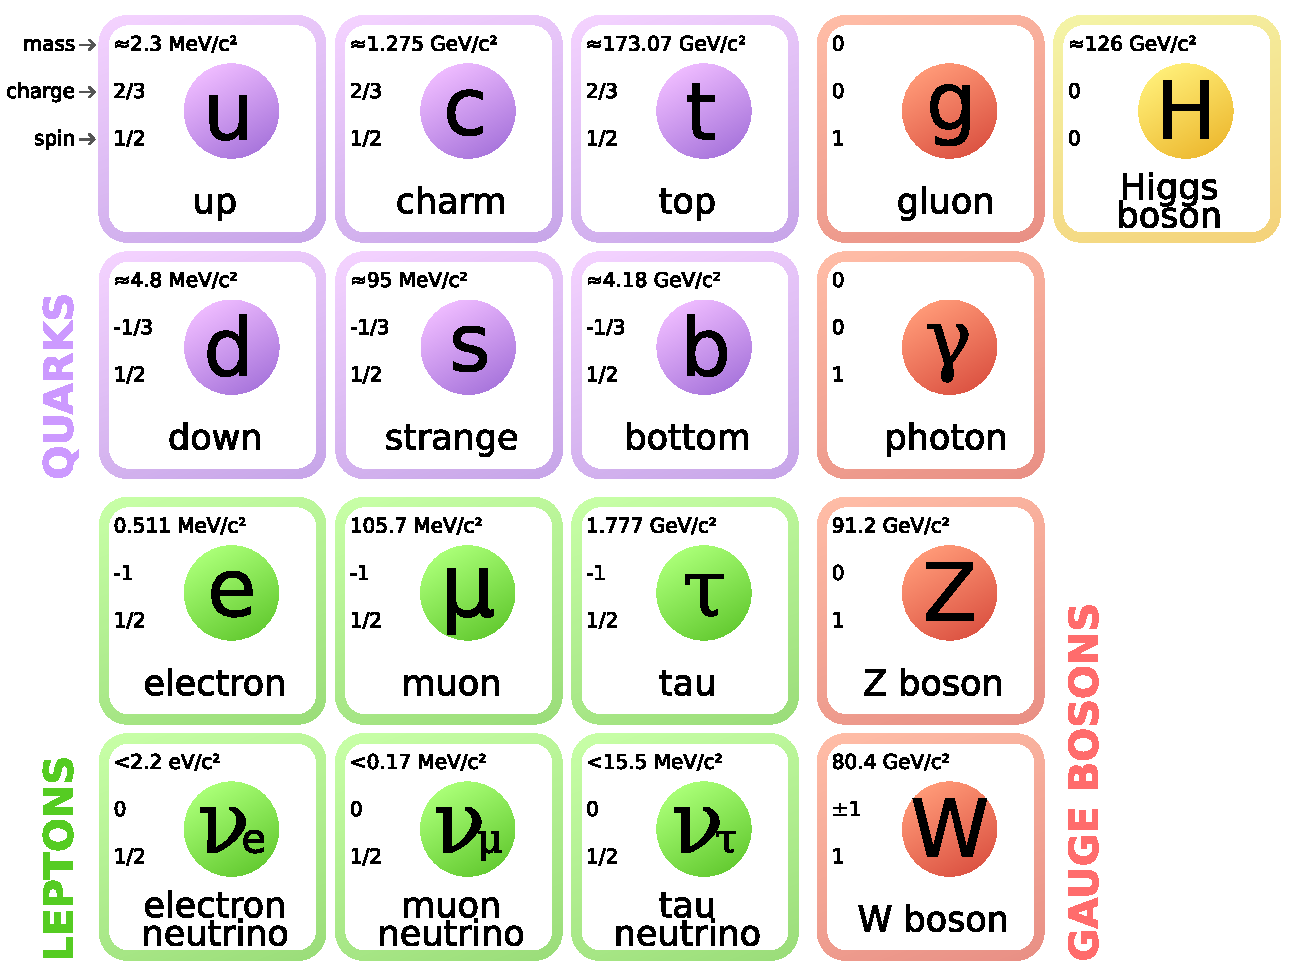
\includegraphics[width=0.9\textwidth]{plots/Standard_Model_of_Elementary_Particles.pdf}
  \caption{The Standard Model's particle content including the latest values~\cite{stdmdlparticles,pdg}.}
  \label{fig:standardmodel}
\end{figure}

\noindent The current ``particle-zoo'', as people like to call the collection of the Standard Model's components, divides all particles into two groups by sorting them based on their spin attribute. The ones with half integer spin are called fermions, while the ones with integer spin are called bosons. The fermion subgroup is once again divided into leptons and quarks, which are grouped into three families each.

Each \textbf{lepton} family is a doublet consisting of a charged $( l, Q_e = -1 )$ and a neutral particle $( \nu_l, Q_e = 0 )$. The doublets have the following particle content:

\begin{equation*}
  \begin{pmatrix}
    \nu_e \\
    e
  \end{pmatrix}
  \quad , \quad
  \begin{pmatrix}
    \nu_\mu \\
    \mu
  \end{pmatrix}
  \quad , \quad
  \begin{pmatrix}
    \nu_\tau \\
    \tau
  \end{pmatrix}
\end{equation*}

The first family is home to the most famous component of the Standard Model, the electron $e$. It is accompanied by the electron neutrino $\nu_e$. Every subsequent family consists of members with the same properties, except for their higher mass. They are named muons $\mu$ and muon neutrinos $\nu_\mu$, as well as taus $\tau$ and tau neutrinos $\nu_\tau$. Due to the mass hierarchy, particles from the higher families usually decay into one of the lower ones, for example $\mu \rightarrow e + \bar{\nu}_e + \nu_\mu$. The main difference between the partner particles of every family, aside from their charge, is the way their interact with matter. While electrons interact with almost anything on a very regular basis, neutrinos are barely noticeable due to their seldom interactions and have gone undetected for more than 20 years after their existence has been proposed.

\textbf{Quarks} do not harbour such fundamental differences between each other. Each family consists of an up-type $( q_u, Q_e = -\frac{2}{3} )$ and a down-type $( q_d, Q_e = +\frac{1}{3} )$ particle. 

\begin{equation*}
  \begin{pmatrix}
    u \\
    d
  \end{pmatrix}
  \quad , \quad
  \begin{pmatrix}
    s \\
    c
  \end{pmatrix}
  \quad , \quad
  \begin{pmatrix}
    t \\
    b
  \end{pmatrix}
\end{equation*}

The first family has the up- and down-flavoured quarks $u$ and $d$, respectively. Similarly to the lepton families, every subsequent family differs only by their increasing mass. Their names are strange $s$ and charm $c$, as well as top $t$ and bottom $b$. Decays like $(udd) \rightarrow (uud) + e + \bar{\nu}_e$ from a higher family to a lower one are also possible. Quarks, as opposed to leptons, cannot be observed in a free state. They are always found in bound states which consist of two or three quarks, which are named mesons and baryons. While the two-quark states are unstable, certain baryons such as the proton $(uud)$ and neutron $(udd)$ are stable over longer periods of time.


While baryons and leptons can join to create atoms and therefore matter, \textbf{bosons} are necessary for the interactions between said particles. Each of the five bosons is responsible for mediating one type of force.

\begin{figure}
  \centering
  \begin{tabular}{ | l | l | c | c | }
    \hline
    Force               & Mediator              & Relative Strength     & Range [m] \\ \hline
    Strong              & Gluons $g$            & $10$                  & $10^{-15}$  \\
    Electromagnetic     & Photons $\gamma$      & $10^{-2}$              & $\infty$  \\
    Weak                & $W$ \& $Z$ bosons     & $10^{-13}$             & $10^{-18}$  \\
    Gravitation         & Graviton $G$          & $10^{-42}$             & $\infty$  \\
    \hline  
  \end{tabular}
  \caption{The four fundamental forces and their attributes. ``Strength'' is to be taken as a rough estimate, as it ultimately is an ambiguous quantity. It depends on the nature of the source and what it is applied on.}
  \label{tab:fundforces}
\end{figure}

For electromagnetic interactions, such as electron pair production and annihilation $e^+ e^- \rightarrow \gamma \rightarrow e^+ e^-$, the photon $\gamma$ is the mediator. The strong force's gluons $g$ mediate interactions between quarks. They are able to bind quarks (e.g. of a proton) despite the electromagnetic repulsion, due to it being a 100 times stronger at that scale. The weak force is mediated by the two vector bosons $W$ and $Z$. Unlike the other forces, the weak one is able to change the flavour of quarks (even violating the otherwise conserved family number) and leptons. Gravitons $G$ have been predicted, but not yet observed. Gravitation is the only fundamental force with a long range, which does not have a repulsive component, as there are no negative masses. Along with its infinite range, it therefore dominates on large, cosmic scales and is responsible for the formation of galaxies and their substructures. Since there is no quantized formulation of the gravitational force, it is not part of the Standard Model.


For every particle there is also a corresponding antiparticle. Antiparticles have the same properties as their normal counterparts, except for their charge-like properties. For example a negatively charged electron $(Q_e = -1)$ has a positively charged $(Q_e = +1)$ antiparticle called the positron. For uncharged particles, this means that they are their own antiparticle. Collisions between a particle and its counterpart usually leads to ``annihilation''. As the name suggests, this leads to both objects being destroyed. Particles produced in this annihilation carry the energy, which is set free in the process. Taking the electron-positron annihilation as an example, the resulting photon can also produce matter once again, it has enough energy. At least the rest mass of both particles in terms of energy is necessary. This means for the aforementioned example that an electron-positron production (``pair production'') is possible, but not necessarily the only option. Similarly muons, taus or quarks could have been the result as long as the charge-like properties are being conserved in the process.


\subsection{Gauge Symmetry}

The Standard Model of particle physics is a relativistic gauge theory, which is invariant under local gauge transformations. Similarly to the Euler-Lagrange approach to classical mechanics

\begin{equation}
  \label{eq:eulerlagrange}
  \frac{d}{dt} \left( \frac{\partial L}{\partial \dot{q}_i} \right) =  \frac{\partial L}{\partial q_i} \quad \text{with } L = T - U,
\end{equation}

\noindent relativistic field theories are formulated using a Lagrangian (density) $\mathcal{L} ( \phi_i, \partial_\mu \phi_i )$, which is a function of time and spatial coordinates as well as its derivatives. It is a necessary transition from a classical particle to a quantized object. The equation using this Langrangian has the following shape.

\begin{equation}
  \label{eq:lagrangian}
  \partial_\mu \left( \frac{\partial \mathcal{L}}{\partial (\partial_\mu \phi_i)} \right) = \frac{\partial \mathcal{L}}{\partial \phi_i} \quad (i = 1, 2, 3, 4)
\end{equation}

Further studies using this equation have lead to the formulation of the weak, strong and electromagnetic force as gauge theories. 

\subsection{Local Gauge Invariance}

The most basic Lagrangian for a spin $\frac{1}{2}$ particle is called a ``Dirac Lagrangian''. It describes a free particle with no external fields:

\begin{equation}
  \label{eq:diraclagrangian}
  \mathcal{L} = i (\hbar c) \bar{\psi} \gamma^\mu \partial_\mu \psi - (m c^2) \bar{\psi} \psi
\end{equation}

\noindent Here the $\psi$ are called ``Spinors'' and are the most basic description of a particle. One can see that under a global gauge transformation, similarly to adding a phase,

\begin{equation}
  \label{eq:globalgaugeinv}
  \psi \rightarrow e^{i \theta} \psi
\end{equation}

\noindent the equation remains invariant. The sign of the exponent will change with complex conjugation and both exponential functions will cancel each other out. Considering that physics should not depend on the location (disregarding external factors), requiring local gauge invariance is necessary:

\begin{equation}
  \label{eq:localgaugeinv}
  \psi \rightarrow e^{i \theta(x)} \psi
\end{equation}

\noindent Doing so will however yield additional terms stemming from the derivation of $e^{i \theta(x)}$ which need to be dealt with. 

\subsection{Quantum Electro Dynamics}
\label{sec:qed}

To compensate for the terms added by requiring local gauge invariance, the covariant derivation is introduced:

\begin{align}
  \label{eq:covariantderivative}
  \mathcal{D}_\mu = \partial_\mu + i \frac{q}{\hbar c} A_\mu
\end{align}

\noindent Using equation~(\ref{eq:covariantderivative}), the invariance of the Lagrangian is restored, but it also adds a spin-1 vector field $A_\mu$, which requires its own additional terms. The basic Lagrangian for such a field is given by:

\begin{equation}
  \label{eq:procalagrangian}
  \mathcal{L} = - \frac{1}{16 \pi} F^{\mu \nu} F_{\mu \nu} + \frac{1}{8 \pi} \left( \frac{m_A c}{\hbar} \right)^2 A^\nu A_\nu - \frac{1}{c} \underbrace{J^\mu}_{Source} A_\mu \quad \text{with } F^{\mu \nu} = \partial^\mu A^\nu - \partial^\nu A^\mu
\end{equation}

\noindent While the first and the last term are locally gauge invariant, the middle one is not. This necessitates a massless mediator $m_A = 0$ to conserve the invariance. Adding both components of the Lagrangians results in

\begin{equation}
  \label{eq:qedlagrangian}
  \mathcal{L}_{\text{QED}} = i (\hbar c) \bar{\psi} \gamma^\mu \partial_\mu \psi - (m c^2) \bar{\psi} \psi - \frac{1}{16 \pi} F^{\mu \nu} F_{\mu \nu} - \frac{1}{c} \underbrace{J^\mu}_{Source} A_\mu,
\end{equation}

\noindent which is the Lagrangian for quantum electro dynamics. So by requiring local gauge invariance under a transformation $\psi \rightarrow U \psi$ with a unitary $1 \times 1$ matrix $U$, here $U = e^{i \theta}$, the photon as the mediator of the electromagnetic force is introduced to the free Lagrangian. It is massless, has a spin of 1 and since its transformation does commutate, it does not interact with other photons. The latter aspect is also coherent with the photon not carrying any charge. The group of all such transformations is called $U(1)$. Using the same principle but different groups of transformations, the remaining interactions will be introduced as well.

\subsection{Quantum Chromo Dynamics}
\label{sec:qcd}

Expanding local gauge invariance from unitary $1 \times 1$ transformations $U(1)$ to the special unitary group $SU(3) = U(1) \otimes U(3)$, one adds the strong interaction to the Lagrangian. The generators of the $SU(3)$ $T_a$ can be described using the Gell-Mann matrices $\lambda_a$ using the relation $T_a = \lambda_a / 2$ with $a = 1, ..., 8$. The important difference between these two groups of transformations is that the $SU(3)$ is not abelian, but adheres the commutation relations given by

\begin{equation}
  \label{eq:qcdgencommute}
  \left[ T_a, T_b \right] = i \sum_{c=1}^8 f_{abc} T_c,
\end{equation}

\noindent where $f_{abc}$ is the structure constant of the $SU(3)$. The previously single component spinors $\psi$ now carry the colour charge and are extended as follows:

\begin{equation}
  \label{eq:colorspinor}
  \psi \rightarrow \psi = \begin{pmatrix}
    \psi_r \\
    \psi_g \\
    \psi_b
  \end{pmatrix}
\end{equation}

\noindent Requiring local gauge invariance results once again in new gauge fields, similarly to QED (Sec.~\ref{sec:qed}). These 8 new fields correspond their respective gluons. Since the transformation is not abelian, these mediators self-couple. This means that they carry a colour charge. The reason for the naming scheme being borrowed from chromatics, is due to the way particles couple. You can only observe colour neutral states. This means that a quark, which are the only fermions to carry a colour charge in the Standard Model, has two options. Either couple to a quark of its anticolour or two other quarks, who carry the remaining two colour charges of the $r,g,b$ triplet. Keeping the titles from section~\ref{sec:stdmdloverview} in mind, those are called mesons and baryons respectively.

Another important aspect of QCD that stems from the self-coupling of gluons, is the behaviour of the strong coupling constant $\alpha_s(Q^2)$. Since it decreases as function of rising momentum transfer $Q^2$, the particles become less constrained the higher the energy scale of the interaction. This is called ``asymptotic freedom'' and can be described pertubatively. On the other end of the scale, around $\sqrt{Q^2} \sim 200\,\text{MeV}$, $\alpha_s{Q^2}$ becomes very large and this freedom turns into ``confinement''. Here the pertubation theory diverges and quarks as well as gluons do not appear as free particles anymore.

\subsection{Electro Weak Theory}

Unlike both the electromagnetic and strong interaction, the weak force has two different ``types'' of interactions. The neutral current (NC) interactions are mediated by the $Z$-boson and behave very similarly to the ones based on an exchange of photons $\gamma$. Charged current (CC) interactions have $W^\pm$ as their gauge boson and contrary to all other types of interactions, it allows for changes of flavour.

Historically, the discovery of the charged currents precedes the one of neutral ones. To describe it as a gauge theory, the symmetry group $SU(2)_L$ is being used. The index ``L'' indicates that these types of currents only couple to left-handed and therefore violates parity conservation maximally. In reference to the spin and isospin attributes, the charge of this interaction is called ``weak isospin'' $I^3$. Using the weak isospin, left-handed particles can be sorted into doublets with $e^-_L$ and $u_L$ having $(I = \frac{1}{2}, I^3 = -\frac{1}{2})$, as well as $\nu_L$ and $d_L$ having $(I = \frac{1}{2}, I^3 = +\frac{1}{2})$. Since right-handed particles do not partake in the charged current interaction, they are sorted into singlets with $(I = 0, I^3 = 0)$.


Using the $SU(2)_L$ symmetry group, yields a third weak interaction. As this still only couples to left-handed particles, it cannot be the weak neutral current which couples to both types. Instead a generator called ``hypercharge'' $Y$ is introduced and defined by:

\begin{align}
  \label{eq:hypercharge}
                  Q_e &= I^3 + \frac{Y}{2} \\
  \Leftrightarrow Y   &= 2 \left( Q_e - I^3 \right)
\end{align}

\noindent This extends the symmetry group by a $U(1)_Y$, thus being $SU(2)_L \otimes U(1)_Y$. The resulting gauge fields are called $W^i_\mu, i = 1,2,3$ for the $SU(2)_L$ and $B_\mu$ for the $U(1)_Y$. These gauge fields mix into two charged and two neutral bosons:

\begin{align}
  \label{eq:ewbosons}
  W^\pm_\mu & = \sqrt{\frac{1}{2}} \left( W^1_\mu \mp W^2_\mu \right) \\
  A_\mu & = \ B_\mu \cos{\theta_W} + W^3_\mu \sin{\theta_W} \\
  Z_\mu & = - B_\mu \sin{\theta_W} + W^3_\mu \cos{\theta_W}
\end{align}
 
\noindent The mixing-angle $\theta_W$ is a free parameter of the Standard Model, meaning that it cannot be predicted from its theoretical construct and has to be measured instead. While the $W^\pm$ and $Z$ bosons are represented by their respective fields, $A_\mu$ can be recognized as the photon introduced in QED (Sec.~\ref{sec:qed}). The electroweak theory therefore describes the combination of both the electromagnetic and weak interaction by unifying them into a single gauge theory.


The Standard Model of particle physics describes nature very well. One of the most precise measurements (and tests of QED), is the ``g-factor'' of the electron's magnetic momentum. While the agreement between theory and experiment can be as good as multiple orders of magnitude as in the aforementioned case, there are still certain discrepancies between theory and experiment in the Standard Model. One of them will be addressed in the following section.

\subsection{The Higgs Mechanism}
\label{sec:higgs}

While the initial two mediators of the respective gauge theories were massless, the $W$ and $Z$ bosons are not. In fact, they are quite heavy with roughly $80.4\,\text{GeV}$ for the $W$ and $90.2\,\text{GeV}$ for the $Z$. This means that the mass terms for both bosons do not vanish and therefore the local gauge invariance, as described in the QED section (Sec.~\ref{sec:qed}), is violated. To alleviate this issue, the concept of ``spontaneous symmetry breaking'' can be used. For this purpose a new field is introduced to the Lagrangian:

\begin{equation}
  \label{eq:higgslagrangian}
  \mathcal{L} =  \frac{1}{2} (\partial_\mu H)^* (\partial^\mu H)  + \frac{1}{2} \mu^2 (H^* H) - \frac{1}{4} \lambda^2 (H^* H)^2
\end{equation}

\noindent Unlike the spinors used in the previous equations, the field $H$ is imaginary and scalar.

\begin{equation}
  \label{eq:higgsimfield}
  H = H_1 + i H_2.
\end{equation}

\noindent While spatial symmetry $H \rightarrow - H$ is maintained, the same cannot be said for the ground state anymore. As shown in figure~\ref{fig:higgspotential}, a unique, non-symmetrical ground state can be attained through spontaneous symmetry breaking.


\begin{figure}[ht!]
  \centering
    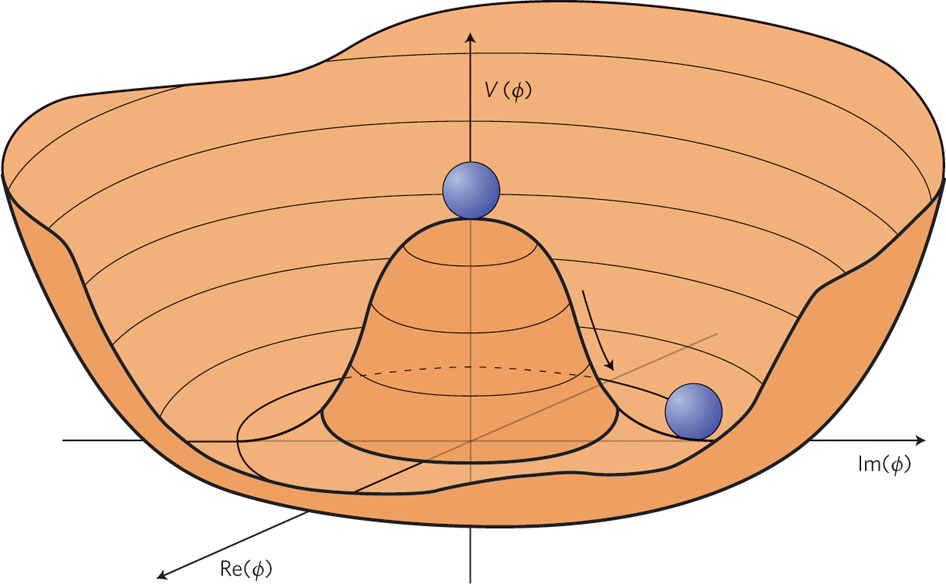
\includegraphics[width=0.5\textwidth]{plots/higgspotential.jpg}
  \caption{The potential of the Higgs-Lagrangian. It is shown how through spontaneous symmetry breaking a non-symmetric ground state can be chosen~\cite{higgspotential}.}
  \label{fig:higgspotential}
\end{figure}


This extension to the theory described by the Lagrangian was suggested by Peter Higgs, who also lends his name to the ``Higgs-boson''. The masses of particles depend on their coupling to the Higgs-field. The stronger the coupling, the higher the mass. As the Higgs-boson also couples to itself, it is massive, too.

The search for the Higgs boson by the CMS collaboration at the Large Hadron Collider has found statistically significant evidence for the existence of a new boson (which resembles the proposed Higgs boson very closely). While previous publications have already shown a $5 \sigma$ excess around the invariant mass of $m_X = 125\,\text{GeV}$~\cite{higgscls}, further studies have been performed on the $H \rightarrow ZZ$ decay mode. Taken from their publication of the 29th of December in 2012, one can see the invariant mass of four selected leptons $m_{4 l}$ in figure~\ref{fig:higgsmzz}.

\begin{figure}[ht!]
  \centering
    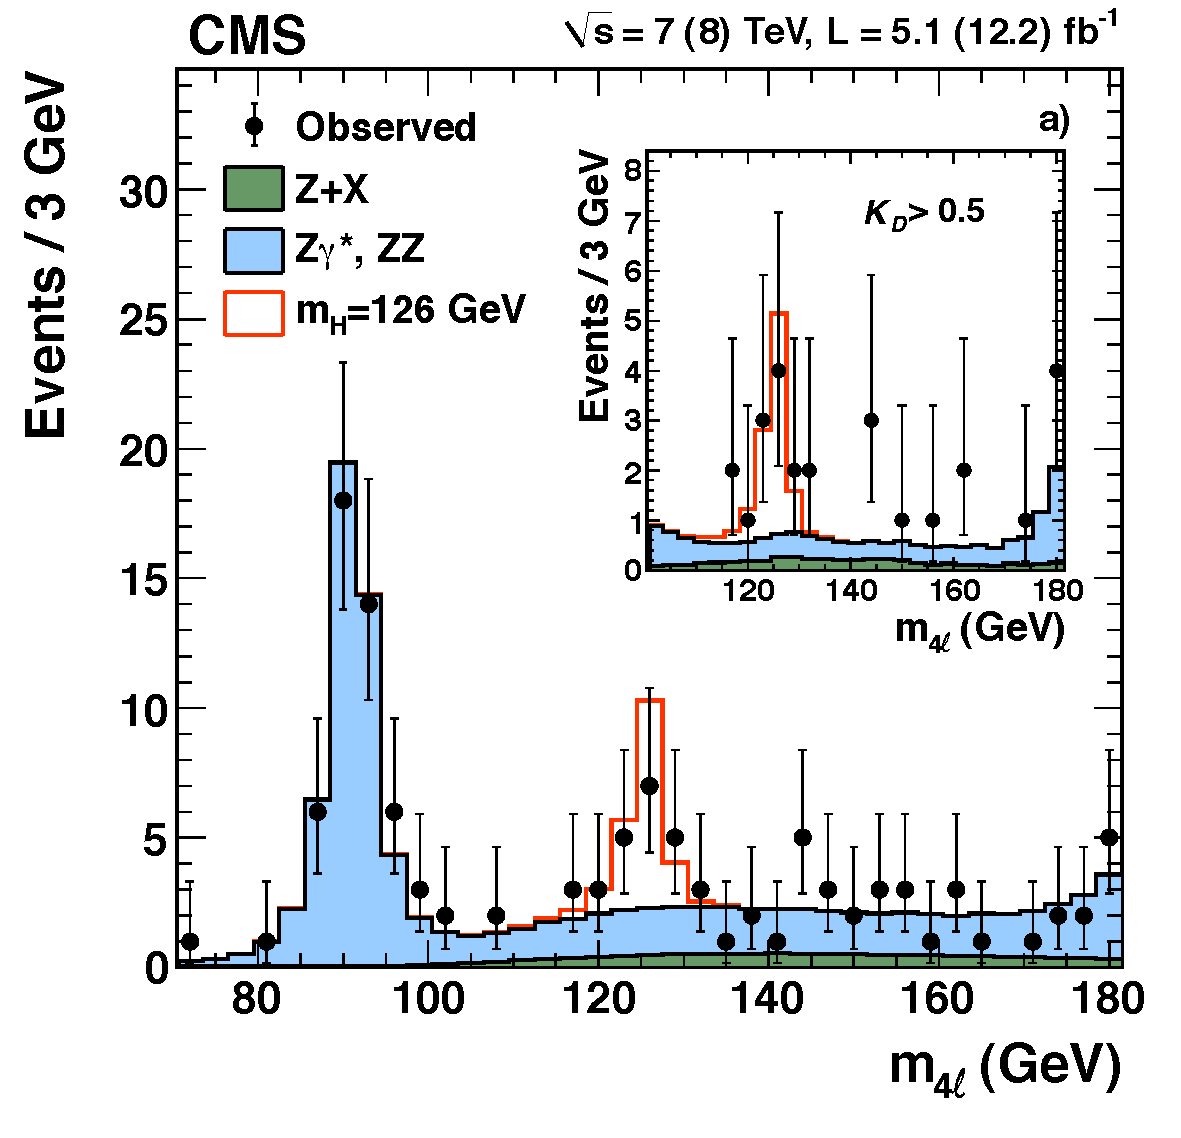
\includegraphics[width=0.6\textwidth]{plots/higgsmzz.pdf}
  \caption{Invariant mass of 4 leptons around the $125\,\text{GeV}$ area, where an excess was observed beforehand~\cite{higgsmzz}.}
  \label{fig:higgsmzz}
\end{figure}

\noindent Combining the results from the $H \rightarrow ZZ$ decay channel with the $H \rightarrow \gamma \gamma$ one, which are the two channels with the best mass resolution, yields the current best mass estimate of $125.8 \pm 0.4 \,\text{(stat)} \pm 0.4\,\text{(syst)}\,\text{GeV}$~\cite{higgsmzz}.


%%% Local Variables: 
%%% mode: latex
%%% TeX-master: "document"
%%% End: 
 % note the page numbering and pagestyle being set inside this include
\section{Supersymmetry}

With a well understood background, discussed in the previous section, one can progress on to physics beyond the Standard Model. One of the most popular and well researched extensions is ``supersymmetry'', often abbreviated as ``SUSY''. This section is based upon the ``Supersymmetry Primer'' by Stephen P. Martin~\cite{susyprimer} and for the particular topic of $R$-parity violation, the work of Herbi Dreiner as well.

\subsection{Motivation}

While the Standard Model describes a multitude of phenomena, there are still certain discrepancies and questions left unanswered. One of the reasons why supersymmetry has gotten as much attention as it has, is because it addresses some of these issues. Three of them will be outlined in the following sections.

\subsubsection{Dark Matter}
\label{sec:dm}

Observation of the universe has lead to the conclusion, that matter as we know it only contributes roughly $5\%$ to the entire energy content. Several different methods have independently discovered phenomena that require a new type of matter. Figure~\ref{fig:gravlens} is showing the ``Bullet Cluster'', which is a prime example of dark matter observation through its gravitational lensing.

\begin{figure}[ht!]
  \centering
  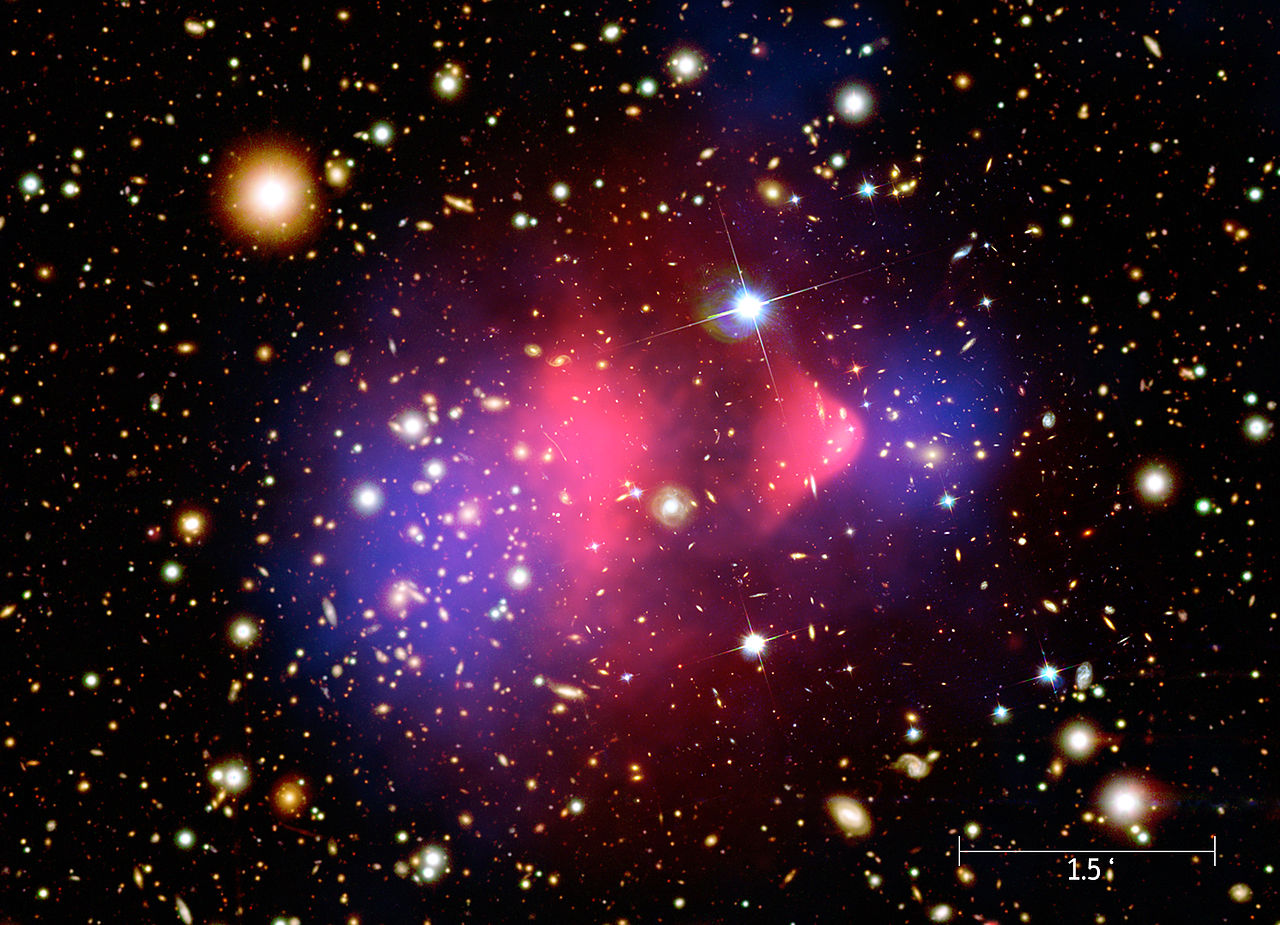
\includegraphics[width=0.6\textwidth]{plots/bulletcluster.jpg}
  \caption{Optical picture of the Bullet Cluster \cite{gravlens}. Two galaxy clusters collided, with the baryonic gas, here marked in red, being slowed down. The dark matter, here marked in blue, passed through and is visible through gravitational lensing.}
  \label{fig:gravlens}
\end{figure}

\noindent Measuring the rotation velocities of stars or gas as a function of their distance to the galaxy's core, also hints at a different type of matter. This is due to the fact, that visible matter itself would not be able to gravitationally bind objects of such high velocities at the observed distances to the galaxy. However adding an additional halo of (\textit{invisible}) matter could provide the necessary additional gravitational force.

As this new type of matter has only been observed indirectly through its effect on nearby structures, it cannot be emitting photons (hence the name \textit{dark} matter) or have a strong impact on cosmic rays. This leads to the assumption that only gravity and possibly the weak force may couple to it. Other interactions\footnote{``Other interactions'' do not include the electromagnetic one, as this would lead to direct optical observation. However, possible interactions that have yet to be discovered are an option as well.} are also within the realms of possibility, but would also necessitate a coupling not stronger than the weak one. These requirements seem to fit the description of the neutrino, but as dark matter tends to cluster, its particles have to be massive and a lot slower.

One possible solution to the question what dark matter consists of are ``Weakly Interacting Massive Particles''. Often abbreviated as ``WIMPs''. The naming is self-explanatory. And while there are no candidates for this role in the Standard Model, supersymmetry does provide suitable particles. The most popular option amongst those, is the lightest supersymmetric particle or LSP, in case it is stable. As the mass hierarchy of supersymmetric particles can change depending on the parameters one chooses, there is not a set LSP. And while not all possible LSPs are considered WIMP candidates, some fit surprisingly well. Should supersymmetry be realized in nature and provide such an explanation for dark matter, it could solve one of the biggest mysteries in cosmology.



\subsubsection{The Hierarchy Problem}
\label{sec:hierprob}
Looking at the large differences in scales between the strength of the gravitational and the weak force (Tab.~\ref{tab:fundforces}), one inevitably expects to see new physics when approaching the point where gravity becomes non-negligible on a quantum level. Considering that the mass of the Higgs boson is of the order $\mathcal{O}(100\,\text{GeV})$ and couples to every massive particle, comparatively huge quantum corrections from heavy particles should contribute to its bare mass $\mu$ (Eq.~\ref{eq:higgslagrangian}). The Yukawa coupling to the Higgs field of an arbitrary fermion is given by

\begin{equation}
  \label{eq:yukawacoup}
  \mathcal{L}_{\text{Yukawa}} = - \lambda_f \bar{\psi} H \psi.
\end{equation}

\noindent Here, $\lambda_f$ denotes the coupling strength. The quantum loop correction of a fermion is depicted in figure~\ref{fig:higgsfloop}.

\begin{figure}[ht!]
  \centering
  \begin{subfigure}[b]{0.49\textwidth}
    \centering
    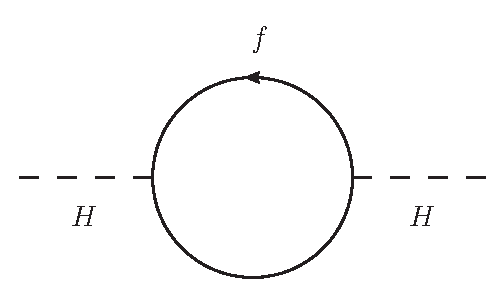
\includegraphics[width=0.6\textwidth]{plots/higgsfloop.pdf}
    \caption{}
    \label{fig:higgsfloop}
  \end{subfigure}
  \begin{subfigure}[b]{0.49\textwidth}
    \centering
    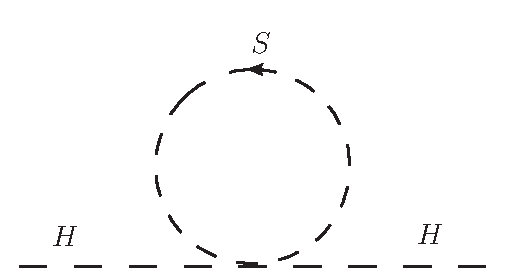
\includegraphics[width=0.6\textwidth]{plots/higgssloop.pdf}
    \caption{}
    \label{fig:higgssloop}
  \end{subfigure}
  \caption{Higgs boson with loop quantum corrections from a fermion \ref{fig:higgsfloop} and a scalar \ref{fig:higgssloop}}
\end{figure}

\noindent Calculating this Feynman diagram yields

\begin{equation}
  \label{eq:higgsfcorr}
  \Delta \mu = - \frac{|\lambda_f|^2}{8 \pi^2} \left[ \Lambda^2_{\text{UV}} + ... \right],
\end{equation}

\noindent where $\Lambda^2_{\text{UV}}$ is the ultraviolet momentum cut-off that is used to stop the loop integral from diverging. It can be interpreted as the scale at which one no longer expects the Standard Model to provide an accurate description of nature any more, meaning that new physics will enter the equation. Assuming this cut-off to be of a much larger scale, e.g. the Planck scale $M_{\text{P}} = 2.4 \cdot 10^{18}\,\text{GeV}$, this would result in corrections that go beyond 30 orders of magnitude when compared to the $\mathcal{O}(100\,\text{GeV})$ we expect for the Higgs' mass. The degree of precision necessary for this sort of parameter appears to be ``unnatural''.

However, in supersymmetry a scalar partner particle is introduced for every fermion, as well as a fermionic partner for every scalar particle. Assuming the couplings remain symmetrical $\lambda_S = |\lambda|^2$, both loop corrections (Fig. \ref{fig:higgsfloop} \& \ref{fig:higgssloop}) would cancel each other out, because fermions and bosons have opposite sign contributions.

\begin{equation}
  \label{eq:higgscancelcorr}
  \Delta \mu = \frac{1}{8 \pi^2} (\lambda_S - |\lambda_f|^2) \left[ \Lambda^2_{\text{UV}} + ... \right]
\end{equation}

\noindent This would provide a ``natural'' solution to the hierarchy problem and thus make supersymmetry all the more interesting.



\subsubsection{Gauge Coupling Unification}

Similarly to how the electromagnetic and weak force has been unified, the physics community has been looking to combine all four fundamental forces into one theory. As the individual forces show different behaviours at lower energy scales, they have to decouple at certain points. Since the coupling strength parameters $\alpha_i(Q),\ i = 1, 2, 3$ a function of the momentum transfer of the interaction, they intersect at certain energies. Figure \ref{fig:coupq} shows the evolution of $\alpha_i(Q)$ in both the Standard Model, as well as the minimal supersymmetric extension to it. 

\begin{figure}[ht!]
  \centering
  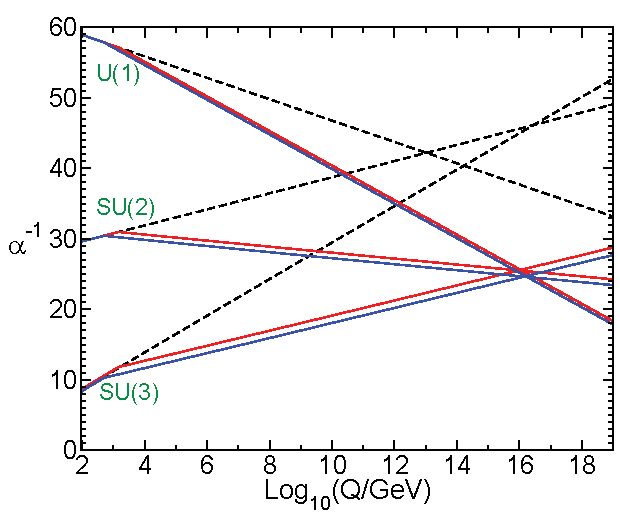
\includegraphics[width=0.6\textwidth]{plots/coupq.pdf}
  \caption{Exemplary evolutions of the inverse gauge couplings $\alpha^{-1}_i(Q)$ through renormalization group equations. The dashed lines show the Standard Model's prediction, while the coloured lines show the one of the Minimal Supersymmetric Standard Model.}
  \label{fig:coupq}
\end{figure}

As one can see, there is no possibility for unification of all three couplings within the Standard Model, while in the extension the points of intersection are in close proximity of each other. Taking the uncertainties of an extrapolation far beyond the reach of current experiments such as this into account, this could hint at an underlying ``grand unified theory'' (\textbf{GUT}). This GUT is, as the name suggests, the previously mentioned effort to unify all the fundamental forces and would be realized around an energy scale of roughly $\sim 10^{18}\,\text{GeV}$.



\subsection{The Minimal Supersymmetric Standard Model}

Symmetries play a huge role in physics. For example a translation in time results in the conservation of energy and a translation in space necessitates momentum to be conserved. In the case of supersymmetry, the quantum property of integer and half-integer spin is being considered as a symmetry. This means relating a fermion to a boson and vice versa. Mathematically speaking an operator that transforms a fermionic state into a bosonic one and back, has to be introduced.

\begin{equation}
  \label{eq:fermiboso}
  Q \Ket{Fermion} = \Ket{Boson}; \quad Q \Ket{Boson} = \Ket{Fermion}
\end{equation}

The new states, which relate to a Standard Model particle each, are called superpartners. As a naming scheme for the partner-particles, the following rules apply. Adding \textit{s-} as a prefix to a fermionic particle's name, yields the title for the scalar superpartner. Using the electron as an example, one gets the selectron. Likewise for scalar particles and their superpartners, the name has to be extended by the suffix \textit{-ino}. The Higgs boson's counterpart would be the Higgsino.

The ``MSSM'', short for ``Minimal Supersymmetric Standard Model'', is the most commonly used and widely studied implementation of supersymmetry. The ``minimal'' expresses itself in the amount of superpartners added to the Lagrangian, which has been kept to the necessary minimum. Usually this means one superpartner for every left-handed and another one for every right-handed particle, which are then sorted into supermultiplets. The Standard Model's Higgs boson is insufficient for the MSSM, as adding just its superpartner would lead to an anomaly in the electroweak gauge symmetry. Thus the number of Higgs eigenstates, as well their supersymmetric counterparts, are extended to four. The supermultiplets of the MSSM are shown in table~\ref{tab:mssmmult}.

\begin{table}[ht!]
  \centering
  \begin{tabular}{| l | c | c | c |}
    \hline
    \multicolumn{2}{ |c| }{ Names }                     & Spin 0        & Spin 1/2 \\ \hline \hline
    \multirow{3}{2.5cm}{(s)quarks $\times 3$~families}  & $Q$           & $\left(\tilde{u}_L \ \tilde{d}_L \right)$     & $\left(u_L \ d_L \right)$ \\
                                                        & $\bar{U}$     & $\tilde{u}_R$                                 & $u_L$ \\
                                                        & $\bar{D}$     & $\tilde{d}_R$                                 & $d_R$ \\ \hline
    \multirow{2}{2.5cm}{(s)leptons $\times 3$~families} & $L$           & $\left(\tilde{\nu}_e \ \tilde{e}_L \right)$   & $\left(\nu_e \ e_L \right)$ \\
                                                        & $\bar{E}$     & $\tilde{e}_R$                                 & $e_R$ \\ \hline
    \multirow{2}{*}{Higgs (-inos)}                      & $H_u$         & $\left(H^+_u \ H^0_u \right)$                  & $\left(\tilde{H}^+_u \ \tilde{H}^0_u \right)$ \\
                                                        & $H_d$         & $\left(H^0_d \ H^-_d \right)$                  & $\left(\tilde{H}^0_d \ \tilde{H}^-_d \right)$ \\ \hline \hline
    \multicolumn{2}{ |l| }{}                            & Spin 1/2      & Spin 1 \\ \hline
    \multicolumn{2}{ |l| }{gluino, gluon}               & $\tilde{g}$   & $g$ \\
    \multicolumn{2}{ |l| }{W (-ino)}                    & $\tilde{W}^{\pm}, W^0$   & $W^{\pm}, W^0$ \\
    \multicolumn{2}{ |l| }{B (-ino)}                    & $\tilde{B}^0$ & $B^0$ \\ \hline
  \end{tabular}
  \caption{Supermultiplets of the Minimal Supersymmetric Standard Model. Left-handed particles are sorted into doublets and right-handed ones into singlets.}
  \label{tab:mssmmult}
\end{table}

Similarly to how the gauge eigenstates $W^i_\mu$ and $B^0_\mu$ mix to their respective mass eigenstates, the mass eigenstates for the MSSM particles also don't always coincide with a single gauge eigenstate. For the first two families of both the sleptons and squarks the mixing is assumed to be negligible. The charged components of the third family however, do have different mass and gauge eigenstates:

\begin{align}
  \label{eq:3fammix}
  \tilde{t}_L \tilde{t}_R & \xrightarrow{\text{\tiny{Mixing}}} \tilde{t}_1 \tilde{t}_2 \\
  \tilde{b}_L \tilde{b}_R & \xrightarrow{\text{\tiny{Mixing}}} \tilde{b}_1 \tilde{b}_2 \\
  \tilde{\tau}_L \tilde{\tau}_R & \xrightarrow{\text{\tiny{Mixing}}} \tilde{\tau}_1 \tilde{\tau}_2
\end{align}

\noindent While in this case the amount of particles remains identical, the electroweak and Higgs gauge bosinos' mass eigenstates can only be sorted by their mass hierarchy and charge:

\begin{align}
  \label{eq:ewhsusymix}
  \tilde{B}^0 \tilde{W}^0 \tilde{H}^0_u \tilde{H}^0_d & \xrightarrow{\text{\tiny{Mixing}}} \tilde{\chi}^0_i \quad \text{with} \quad i = 1,2,3,4 \\
  \tilde{W}^\pm \tilde{H}^+_u \tilde{H}^-_d & \xrightarrow{\text{\tiny{Mixing}}} \tilde{\chi}^\pm_i \quad \text{with} \quad i = 1,2
\end{align}

\noindent As the MSSM also requires new ``Standard Model'' Higgs bosons, these also mix:

\begin{equation}
  \label{eq:hmix}
  H^0_u H^0_d H^+_u H^-_d \xrightarrow{\text{\tiny{Mixing}}} h^0 H^0 A^0 H^\pm
\end{equation}

\noindent The $h^0$ resembles the Standard Model's Higgs closely and therefore the potential Higgs discovery from section~\ref{sec:higgs} does not stand in direct conflict with the MSSM. Gluons and gluinos do not mix.

With the given particle content, the final step of the implementation is modifying the Lagrangian. Integration of the supersymmetric extension into it, requires the superpotential with the respective superfields from table~\ref{tab:mssmmult} to be added.

\begin{equation}
  \label{eq:mssmsuperpot}
  W_{\text{MSSM}} = \bar{U} \mathbf{y_u} Q H_u - \bar{D} \mathbf{y_d} Q H_d - \bar{E} \mathbf{y_e} L H_d + \mu H_u H_d
\end{equation}

\noindent The $\mathbf{y_i}$ with $i = u,d,e$ are the Yukawa coupling parameters. They are $3 \times 3$ matrices in flavour space and determine the mass spectrum. The $\mu$-term is the supersymmetric version of the $\mu$-term in the Higgs mechanism's superpotential (Eq.~\ref{eq:higgslagrangian}).

\subsection{Soft SUSY Breaking}

If supersymmetry would be an exact symmetry, sparticle masses are expected to be identical to their Standard Model counterpart. However, the lack of discoveries of at least the low mass components (e.g. the selectron) necessitates it to be a spontaneously broken symmetry. This means that the supersymmetric partner particles are expected to have masses which are outside the reach of current experiments. One also has to keep in mind, that the ``naturalness'' of the solution to the hierarchy problem (Sec.~\ref{sec:hierprob}) depends on the coupling strengths being equal. To allow the symmetry to be broken while keeping the cancellation of the loop contributions to the Higgs mass, requires the symmetry breaking to be \textit{soft}. This means that the Lagrangian can be written like

\begin{equation}
  \label{eq:softlagr}
  \mathcal{L} = \mathcal{L}_{\text{SUSY}} + \mathcal{L}_{\text{soft}},
\end{equation}

\noindent to split the gauge and Yukawa couplings (SUSY) from the mass terms (soft).


To achieve this distinct shape of the Lagrangian, a new interaction is necessary for which various models have been suggested. \textit{Gravity mediated supersymmetry breaking}, also known as \textit{Planck-scale supersymmetry breaking}, is the most popular one. The general idea is that, through the new physics that enter once gravity becomes relevant on a quantum scale, new gauge bosons mediate the masses of the supersymmetric particles. By requiring supersymmetry to be a local gauge symmetry, similarly to how the electroweak and strong force are implemented, one receives both a graviton (Spin 2) and a gravitino (Spin 3/2). It also yields an additional term for the goldstino, which is absorbed by the gravitino. The latter acquires mass due to the absorption. This theory is called supergravity.

\subsubsection{Constrained Minimal Supersymmetric Standard Model}

The most simple version of supergravity with the least amount of additional particles is called \textit{minimal supergravity} (\textbf{mSUGRA}) or \textit{constrained Minimal Supersymmetric Standard Model} (\textbf{cMSSM}). One of the reasons why this particular realization is popular, is the massive reduction of free parameters it achieves. While there are 105 of them in the MSSM, the scale dependency of the sparticle masses allows for a unification of multiple parameters at the grand unified theory (\textbf{GUT}) scale. Figure~\ref{fig:msugrarge} displays how the individual scalar and fermionic masses converge at the respective points of intersection.

\begin{figure}[ht!]
  \centering
  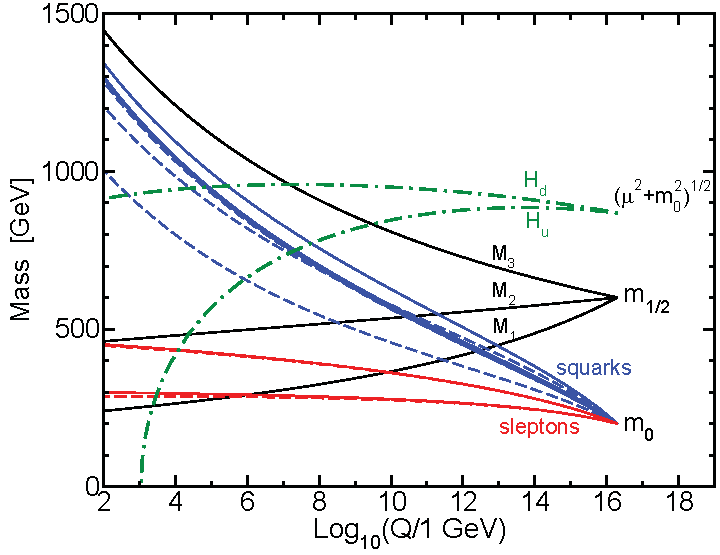
\includegraphics[width=0.7\textwidth]{plots/msugrarge.pdf}
  \caption{Unification of sparticle masses at the GUT scale in the cMSSM, thus allowing for a significantly smaller amount of free parameters.}
  \label{fig:msugrarge}
\end{figure}

\noindent Through the renormalization group equations, it is possible to extrapolate from these points. The remaining 5 parameters are:

\begin{itemize}
\item $m_0$ - Universal mass of scalar sparticles at the GUT scale
\item $m_{1/2}$ - Universal mass of fermionic sparticles at the GUT scale
\item $A_0$ - Trilinear Higgs coupling strength at the GUT scale
\item $\tan{\beta}$ - Tangent of the ratio of the vacuum expectation values of $H^0_u$ \& $H^0_d$
\item $\text{sgn}\,\mu$ - The sign of the bilinear Higgsino mixing parameter
\end{itemize}

\subsection{R-Parity}

When adding the most general version superpotential for the MSSM to the Lagrangian, the theory appears to be consistent at first. However, certain phenomenological discrepancies would be left unaddressed. There are lepton number violating (\textbf{LNV}), as well as baryon number violating (\textbf{BNV}) terms:


\begin{align}
  \label{eq:lnvlagr}
  W_{\text{LNV}} &= \frac{1}{2} \lambda_{ijk} L_i L_j \bar{E}_k + \lambda^\prime_{ijk} L_i Q_j \bar{D}_k + \kappa^{i} L_i H_u \\
  \label{eq:bnvlagr}
  W_{\text{BNV}} &= \frac{1}{2} \lambda^{\prime\prime}_{ijk} \bar{U}_i \bar{D}_j \bar{D}_k
\end{align}


\noindent Here $\lambda$, $\lambda^\prime$, $\lambda^{\prime\prime}$ and $\kappa$ denote the coupling strengths of the the respective interactions between the superfields (see tab.~\ref{tab:mssmmult}). The indices $i$, $j$, and $k$ represent family numbers. These terms would for example lead to rapid proton decay. The latter has an experimental limit at $90\pct$ confidence level of $6.6 \cdot 10^{33}$ years, given by the Super-Kamiokande experiment in Japan~\cite{protondecay}.

To prevent this inconsistency, both types of terms could be suppressed by simply assuming the coupling parameters to be equal to zero. However in the MSSM, instead of simply forcing the theory to adhere to the observation through demanding certain parameters to be set, a new symmetry is introduced. The so called ``$R$-parity'' $P_R$ is a discreet $Z_2$ symmetry and assigns a quantum number to every particle, which can be calculated by:

\begin{equation}
  \label{eq:rparity}
  P_R = (-1)^{3 (B-L) + 2 S}
\end{equation}

\noindent One can easily confirm that every particle has an even $R$-parity ($P_R = +1$), while the supersymmetric counterparts have an odd $R$-parity ($P_R = -1$). Assuming $R$-parity is conserved, supersymmetric particles can only be produced in even numbers (usually pairs). This is due to it being a multiplicative quantum number, which calculates as follows for a vertex. With two particles entering one gets $P_R = (+1) \cdot (+1) = +1$. If they annihilate and produce two sparticles the calculation yields $P_R = (-1) \cdot (-1) = +1$. Obviously under $R$-parity conservation, this could not have produced one sparticle alongside one particle. This also forbids both the lepton and baryon number violating processes (Eq.~\ref{eq:lnvlagr}~\&~\ref{eq:bnvlagr}) and has another major phenomenological consequence. The lightest supersymmetric particle (\textbf{LSP}) has to be stable, as any further decay would require an additional, even lighter supersymmetric particle. Should this LSP be neutral, it would only interact very weakly with baryonic matter. Under these circumstances, supersymmetry could provide a suitable candidate for a WIMP (compare to section~\ref{sec:dm}).



\subsubsection{The Violation of R-Parity}
\label{sec:rparityvio}

While most supersymmetric models do make use of $R$-parity, there is no intrinsic motivation for choosing this symmetry over others who can provide the same phenomenology. It can be shown that there are other, gauge anomaly free $Z_N$ symmetries that can prevent the proton from decaying~\cite{b3p6}. In this analysis baryon-triality $B_3$ is assumed. The discreet symmetry for this scenario is given by~\cite{b3def}

\begin{equation}
  \label{eq:b3symmetry}
  \psi_j \rightarrow e^{\alpha_j 2\pi i/3} \psi_j.
\end{equation}

\noindent The values of $\alpha_j$ for the respective superfields are given in table~\ref{tab:alphaj} below.

\begin{table}[htb]
  \centering
  \begin{tabular}{|c|c|c|c|c|c|c|c|}
    \hline
    & $Q_i$ & $\bar{U}_i$ & $\bar{D}_i$ & $L_i$ & $\bar{E}_i$ & $H_d$ & $H_u$ \\ \hline
    $\alpha_j$ & 0 & 2 & 1 & 2 & 2 & 2 & 1 \\ \hline
  \end{tabular}
  \caption{Values of $\alpha_j$ for the respective superfields in the baryon-triality model.}
  \label{tab:alphaj}
\end{table}

Baryon-triality allows for the lepton number violating terms (Eq.~\ref{eq:lnvlagr}), but forbids baryon number violating ones (Eq.~\ref{eq:bnvlagr}). As a result the proton remains stable, while the LSP is able to decay. Due to the instability of the LSP in RPV supersymmetry, the idea of an LSP being a dark matter candidate has to be abandoned. However, resonant production of sleptons is possible, which can lead to very distinct decay chains (without ``invisible'' particles). This analysis will make use of that.


\subsection{Analysis Model}
\label{sec:anamodel}

As this analysis is focussing on searching for resonant production of sleptons, R-parity has to be violated (cf. sec.~\ref{sec:rparityvio}). To determine the viable couplings through which sleptons (Eq.~\ref{eq:lnvlagr}) can be produced, one has to keep the initial state in mind. For proton-proton collisions this strongly favours the LQD term with $\lambda^\prime_{ijk}$, as it is able to convert two quarks directly into a slepton. With the valence quarks of a proton being of the first generation, their contribution to the coupling will be dominant. While this sets $j = k = 1$, the remaining index determines the generation of the sleptons. Since neutrinoless double beta decay puts strict bounds on the coupling for the first generation $\lambda^\prime_{111}$~\cite{rpvimpl}, searching for the second generation is the more attractive option. Assuming single coupling dominance~\cite{rpvimpl} for $\lambda^\prime_{211}$, contributions from other couplings can be neglected.

\subsubsection{Current Limits}

While $R$-parity conserving scenarios are more popular and therefore more thoroughly investigated, there has also been searches for the particular model this analysis concerns itself with. As none of these searches have had any discoveries, their main results are limits on the value of $\lambda^\prime_{211}$.

\begin{figure}[ht!]
  \centering
  \begin{subfigure}[b]{0.77\textwidth}
    \centering
    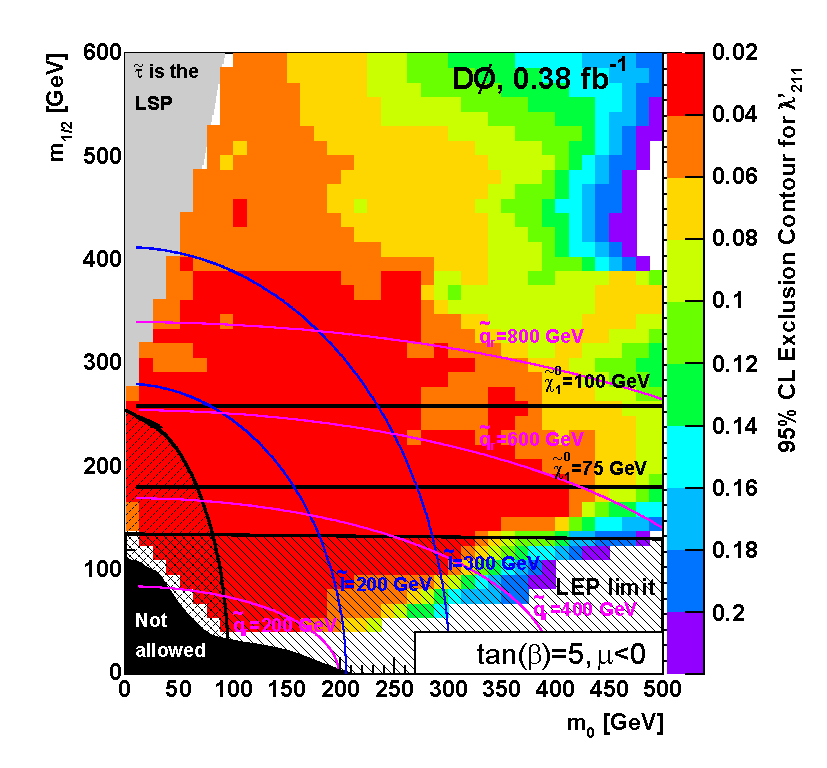
\includegraphics[width=\textwidth]{plots/auterrpv.pdf}
    \caption{\label{fig:auterrpv}}
  \end{subfigure}
  \begin{subfigure}[b]{0.77\textwidth}
    \centering
    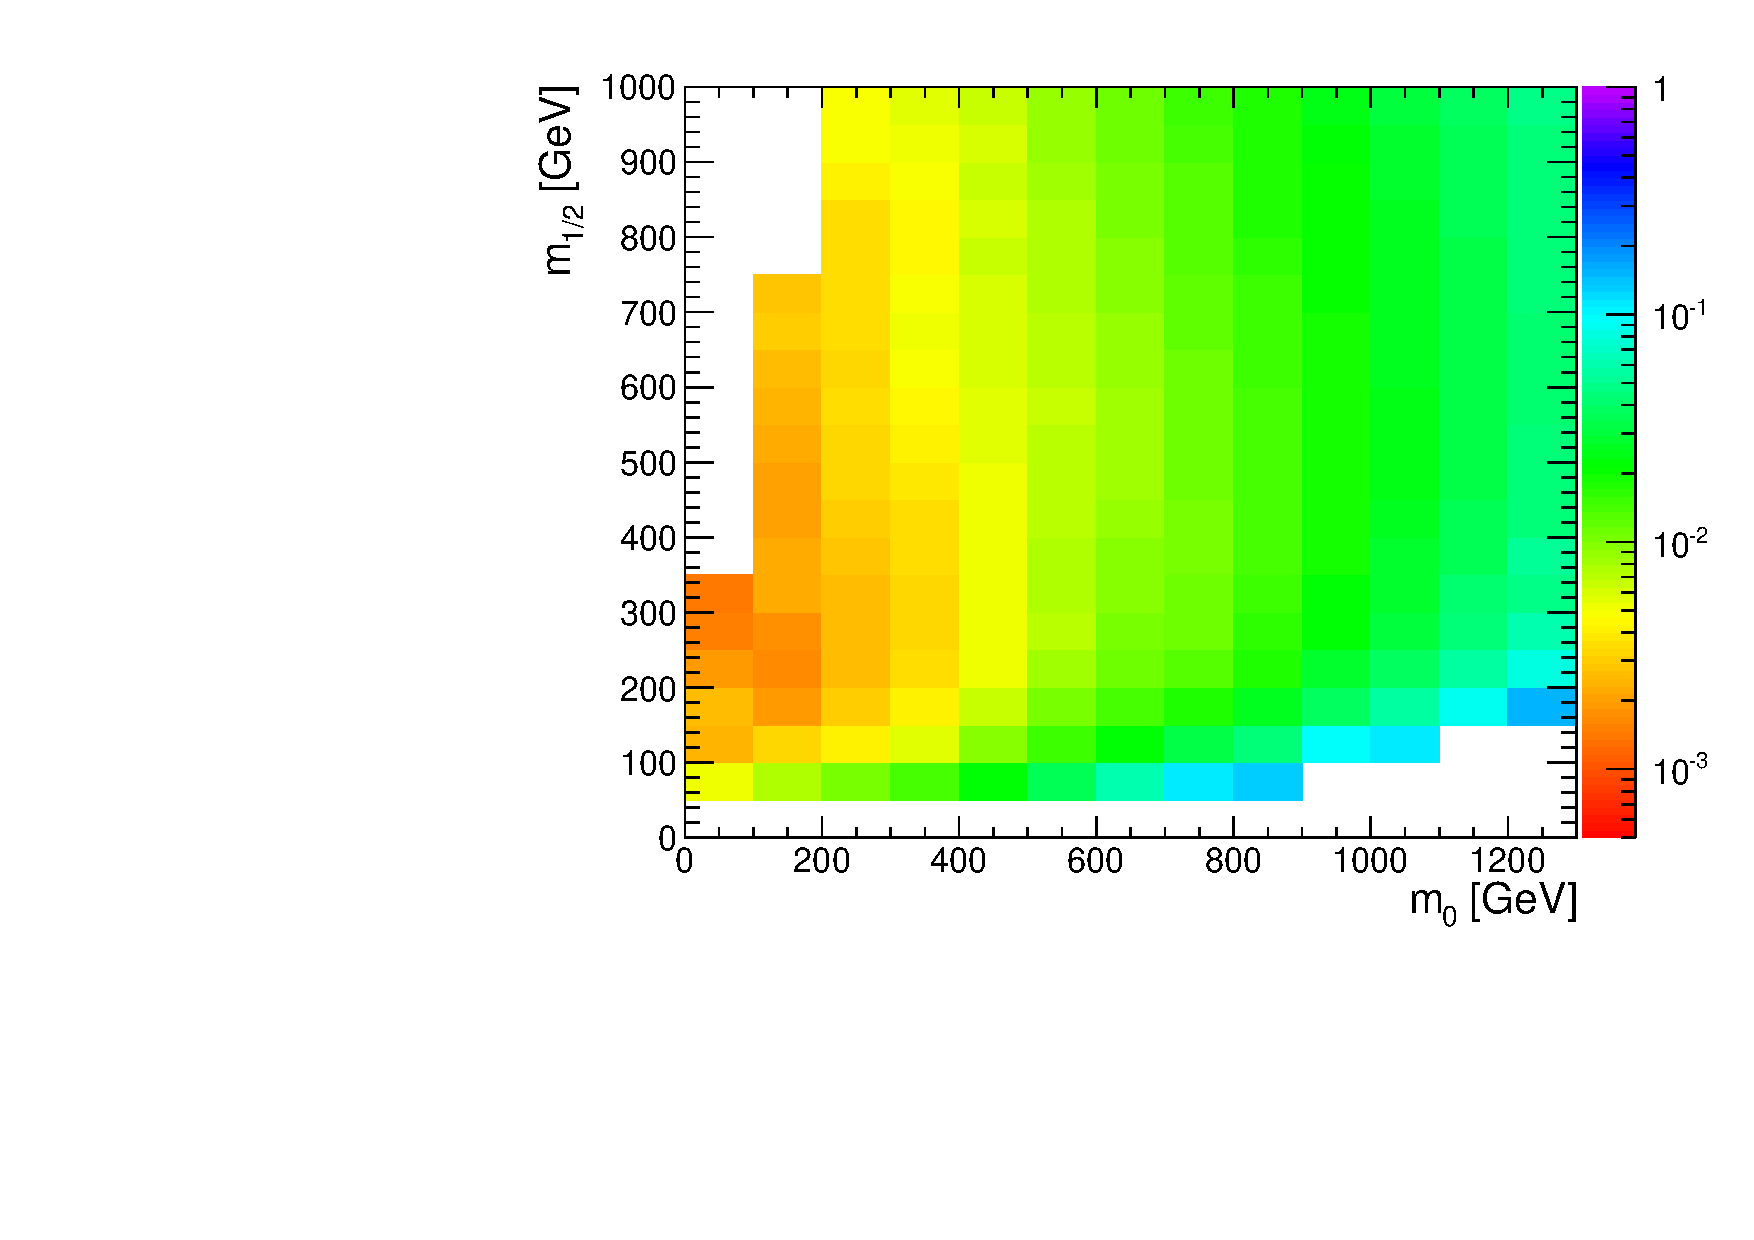
\includegraphics[width=\textwidth]{plots/2011-l211limits_MultiBin_logz-colz.pdf}
    \caption{\label{fig:endresrpv}}
  \end{subfigure}
  \caption{$95\,\%$ C.L. exclusion limits for resonant slepton production through the $\lambda^{\prime}_{211}$ coupling. They have been calculated using the data measured at the D0 experiment (\ref{fig:auterrpv}) at the Tevatron~\cite{auter} and the measurements of CMS experiment at the LHC during 2011, which was operating at a center-of-mass energy of $\sqrt{s} = 7\,\text{TeV}$~\cite{endres}.}
\end{figure}

Figure~\ref{fig:auterrpv} shows the results from the D0 experiment at the Tevatron~\cite{auter,d0rpv}, which were the most stringent limits from a collider experiment prior to the LHC. Shown are the $95\pct$ confidence level exclusion limits that this direct search yielded.

Due to the technically more advanced combination of the LHC and CMS experiment, the results could be expanded upon. Figure~\ref{fig:endresrpv} shows the extended, more strict limits, which were obtained using the data recorded during 2011~\cite{endres}. These exclusion ranges are the basis for this analysis.


%%% Local Variables: 
%%% mode: latex
%%% TeX-master: "document"
%%% End: 

\chapter{The Experiment}
\label{cha:experiment}

The analysis is based upon LHC proton-proton collisions at a centre-of-mass energy of $\sqrt{s} = 8\,\text{TeV}$, which have been recorded by CMS during 2012. This chapter will provide an overview over both the LHC, as well as the CMS experiment.


\section{Large Hadron Collider}
\label{sec:lhc} 

To study the structure of nature at the smallest scales, various particle accelerators with increasingly higher center-of-mass energy have been built. The Large Hadron Collider (\textbf{LHC})~\cite{lhcjinst}, built at the CERN laboratory, is the machine which currently provides the highest beam energies. It resides in a $27.6\,\text{km}$ long, circular tunnel roughly $100\,\text{m}$ underground, near Geneva. As opposed to the Large Electron-Positron collider (\textbf{LEP}) which previously operated in said tunnel, the LHC is designed to work with both protons and heavy ions, such as lead. This effectively allows for much higher centre-of-mass energies, as the synchrotron radiation decreases with increasing masses of the accelerated particles. To stay in line with the analysis' focus on proton-proton collisions, the following sections will also concern themselves with these.

Since most of the interesting interactions are very rare compared to the ones that have already been studied, it is essential for the LHC to produce a sufficient amount of collisions. The instantaneous luminosity $\mathcal{L}$ is a measurement of said rate of production. The expected number of events per second for a certain process is then given by

\begin{equation}
  \label{eq:instlumi}
  N_{\text{Process}} = \mathcal{L} \sigma_{\text{Process}}.
\end{equation}

\noindent Here $\sigma_{\text{Process}}$ denotes the cross-section, which can be interpreted as the probability of the considered process to occur. The design value for the instantaneous luminosity of the LHC is $\mathcal{L} = 10^{34}\,\text{cm}^{-2}\,\text{s}^{-1}$. At the end of the 2012 data taking period, the peak instantaneous stable luminosity recorded by CMS was $7670.19 \cdot 10^{30}\,\text{cm}^{-2}\,\text{s}^{-1}$~\cite{cmslumi}, which is already very close to the design goal.

The LHC has been constructed for a centre-of-mass energy of $\sqrt{s} = 14\,\text{TeV}$, although reaching this design energy has been postponed. With each of the two beams carrying half the energy, only $3.5\,\text{TeV}$ per beam have been reached during 2011. It has been increased to $4.0\,\text{TeV}$ in 2012. This slow start is mostly due to an accident during the start-up of the machine in 2008, which requires (still ongoing) extensive repairs and has lead to redesigning certain components.

The injector chain (Fig.~\ref{fig:injchain}) is responsible for supplying the LHC with protons. After extracting the particles from Hydrogen gas using an electrical field, the $90\,\text{keV}$ protons are boosted to $750\,\text{keV}$ by a radio frequency quadropole (\textbf{RFQ}) before entering a linear accelerator (\textbf{LINAC 2}). With $50\,\text{MeV}$ they are sent to the Proton Synchrotron Booster (\textbf{PSB}), which feeds the Proton Synchrotron (\textbf{PS}) protons with $1.4\,\text{GeV}$ kinetic energy. After being accelerated to $25\,\text{GeV}$ the particles pass through the last pre-accelerator, which is the Super Proton Synchrotron (\textbf{SPS}). As they reach $450\,\text{GeV}$ the trains of bunches are separated into two halves before being injected into the LHC.

\begin{figure}[ht!]
  \centering
  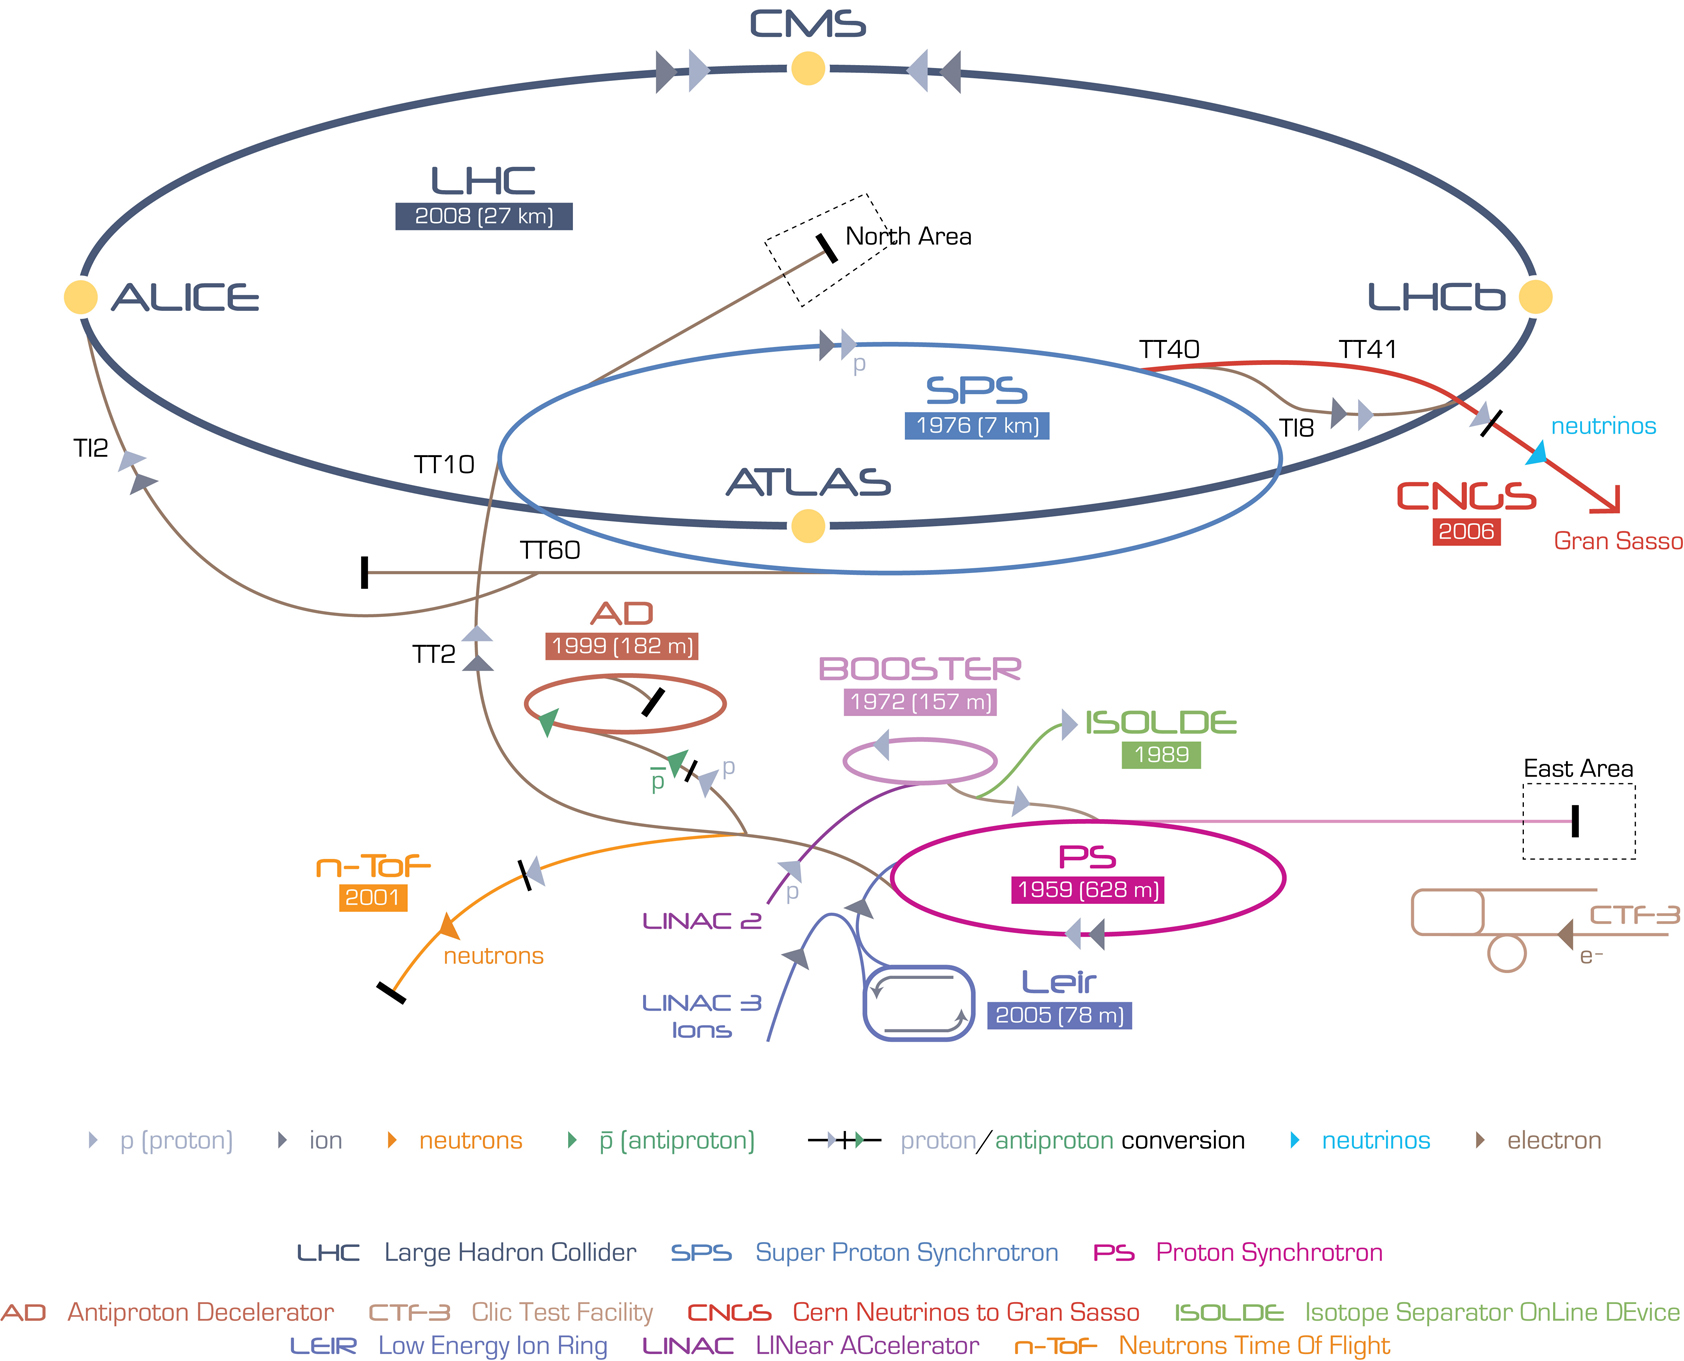
\includegraphics[width=0.8\textwidth]{plots/lhcinjectorchain.jpg}
  \caption{Schematic picture of the injector chain for the LHC~\cite{injchain}.}
  \label{fig:injchain}
\end{figure}

The LHC uses superconducting radio frequency cavities made of niobium to boost the protons to their final energy. Superconducting dipole magnets made of niobium-titanium are used to guide the proton's trajectory. They can reach up to $8\,\text{T}$. Quadrupole, sextupole and octopole magnets are used to clean and focus the beam. The four major experiments are located in caverns, where the two beams are crossing their paths. The ATLAS~\cite{atlasjinst} and CMS~\cite{cmsjinst} experiments are multi-purpose detectors, while ALICE~\cite{alicejinst} is focusing on heavy ions and LHCb~\cite{lhcbjinst} concentrates on b-quark physics.



\section{Compact Muon Solenoid}
\label{sec:cms}

Roughly $100\,\text{m}$ below Cessy, at the fifth interaction point (\textbf{IP5}) of the LHC, the Compact Muon Solenoid (\textbf{CMS})~\cite{cmsjinst} is installed (Fig.~\ref{fig:cms}). The cylindrical shape measures $21.6\,\text{m}$ in length and has a diameter of $14.6\,\text{m}$, with an overall weight of $14\,\text{kT}$. It is composed of a large solenoid magnet and a wide variety of sub-detectors, with a \textit{barrel} and an \textit{endcap} region. In combination, they are designed to measure the energy, momentum and trajectory of the particles. The individual components will be discussed in the upcoming sections.

\begin{figure}[ht!]
  \centering
  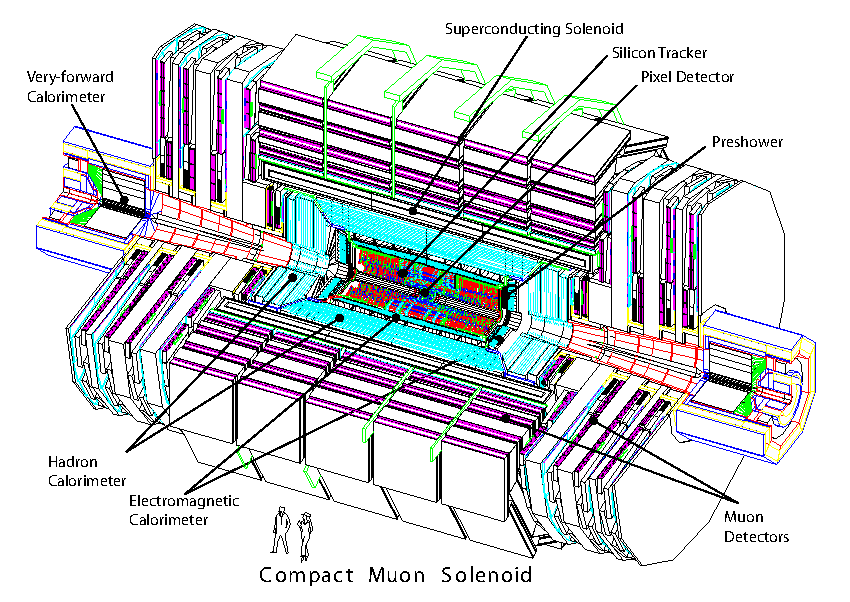
\includegraphics[width=0.8\textwidth]{plots/cms.pdf}
  \caption{Overview of the CMS experiment at the LHC~\cite{cmsjinst}. For a size comparison, two experimentalists are shown.}
  \label{fig:cms}
\end{figure}

The coordinate system chosen by the CMS collaboration places the origin at the nominal collision point of the two proton beams. The $z$-axis is along the path of the proton beams, while the $x$-axis points inward to the center of the LHC ring. That leaves only the vertical, upward direction for the $y$-axis. The radial coordinate $r$ is measured with respect to the nominal interaction point and the azimuth angle $\phi$ is the $x$-$y$ plane. However, instead of the polar angle $\theta$, a quantity called ``pseudorapiditiy'' $\eta$ is being used. It is given by $\eta = - \ln{\text{tan}\,\left(\frac{\theta}{2}\right)}$ and has the advantage of being invariant under longitudinal Lorentz boosts. The latter is very helpful because of the unknown longitudinal initial state of a proton-proton collision, due to protons having a substructure. Thus the frame of reference can always be chosen to be the rest frame, without having to recalculate the polar angle. Using the pseudorapidity, the spatial distance between two objects is defined as

\begin{equation}
  \label{eq:spatdiff}
  \Delta R = \sqrt{\left(\Delta \phi\right)^2 + \left(\Delta \eta\right)^2}.
\end{equation}

\subsection{Magnet}

The shape of the magnet is one of the main choices for an experiment. One has to weigh the trajectory bending power against the area density, where the former is essential to measure particle charge and momenta, while the latter can lead to losing or altering particle information due to various effects. The CMS collaboration chose a solenoid shape and thus having a magnetic field parallel to the beam line. One of the distinct features is the superconducting niobium titanium material organized in a 4-layer structure. With the cold mass of the magnet itself being ``only'' $220\,\text{tons}$, the $10\,000\,\text{ton}$ iron yoke surrounding the magnet from the outside is the main contribution to the overall weight. The iron yoke is necessary to return the magnetic flux to the magnet. With the $3.8\,\text{Tesla}$ the magnet is designed to operate at in the inner detector, it provides excellent bending power. In the muon chambers, its only about $2\,\text{T}$ remain.

\subsection{Inner Tracker}
\label{sec:innertracker}

The inner tracker~(Fig.~\ref{fig:inntrk}) is the detector component closest to the collision point. As such, it is faced with the biggest challenges. With about 20 proton-proton collisions up to every $25\,\text{ns}$, not only an extremely fast response time, but also an excellent spatial resolution is necessary. The radiation damage from said interactions also had to be considered. As a result, a detector based on silicon has been chosen and constructed. It has an expect lifetime of 10 years, after which it has to be replaced. The layout of the inner tracker has two components which will be discussed in the next sections.

\begin{figure}[ht!]
  \centering
  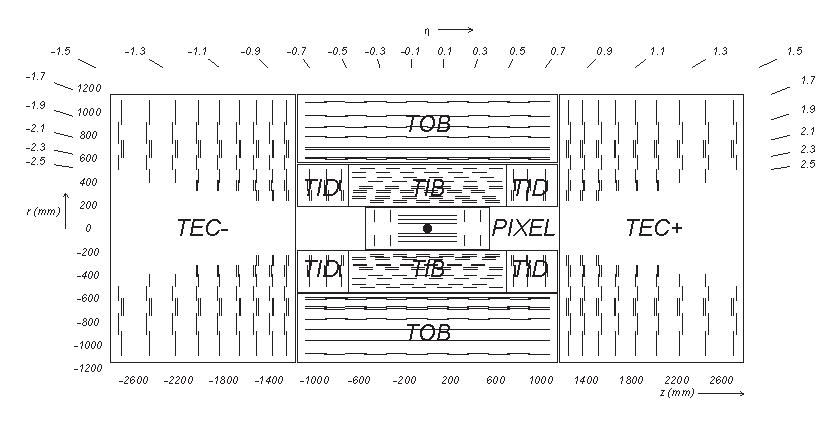
\includegraphics[width=0.8\textwidth]{plots/innertracker.pdf}
  \caption{Layout of the inner tracker of the CMS experiment. Every line represents a silicon detector, whereas the double lines have a secondary micro-strip detector to measure the co-coordinate~\cite{cmsjinst}.}
  \label{fig:inntrk}
\end{figure}

The \textbf{pixel detector} has its three layers at radii of $4.4$, $7.3$ and $10.2\,\text{cm}$ in the barrel region. Two additional discs are positioned on the sides. With an overall amount of $66$ million pixels, it covers an area of roughly $1\,\text{m}^2$. The pixel size of $100 \times 150\,\mu\text{m}^2$ provides an excellent track resolution. This allows for an accurate reconstruction of secondary vertices, giving valuable insight into the decay chains.

Outside of the pixel detector, the \textbf{silicon strip tracker} is extending from $20$ to $116\,\text{cm}$. It has three different subcomponents. The Tracker Inner Barrel (\textbf{TIB}) with its 4 layers and the complementing 3 Tracker Inner Disks (\textbf{TID}) on each side, are positioned parallel and radial to the beam line, respectively. After reaching a radius of $55\,\text{cm}$ the Tracker Outer Barrel (\textbf{TOB}) occupies the remainder of the barrel space with its 6 layers. Following the same structure as the TIB and TID, the endcaps are covered by the Tracker End Caps (\textbf{TEC}), which add another 9 layers of silicon strips. The width and pitch of each strip determine the spatial resolution. It varies between $23$, $35$ and $53\,\mu\text{m}$, with a tendency towards a better resolution the closer the strip is to the collision spot. Additional micro-strip detector modules are attached to the first two layers of the TIB, TID and TOB. Those are used for measuring the respective co-coordinate with a stereo angle of $100\,\text{mrad}$. Overall, the silicon strip tracker has a total of $9.3$ million strips with a surface area of $198\,\text{m}^2$.

Combining both components of the inner tracker, it is possible to measure the transverse momentum of highly energetic tracks with a resolution of $1-2\,\pct$. The geometrical range of $|\eta| < 2.5$ is being covered.


\subsection{Electromagnetic Calorimeter}

As the name suggests, the electromagnetic calorimeter (\textbf{ECAL}) is responsible for measuring electrons and photons. This also includes the electromagnetic component of jets, which is mostly given by $\pi^0 \rightarrow \gamma \gamma$. To achieve good response times, fine granularity\footnote{High density: $8.28\,\text{g/cm}^3$; Short radiation length: $0.89\,\text{cm}$; Small Moli\`{e}re radius: $2.2\,\text{cm}$} and still be resistent to radiation damage, lead tungstate crystals PbWO$_4$ have been chosen.

The barrel region covered by the calorimeter (\textbf{EB}) spans over $|\eta| < 1.479$. A total of 61200 crystals with a cross section of $22 \times 22\,\text{mm}^2$ near the collision point and $26 \times 26\,\text{mm}^2$ furthest from it, have been mounted. It should be noted that with these dimensions, the Moli\`{e}re radius is able to be contained within a cell, resulting in a good spatial resolution. The length of a cell also corresponds to $25.8 X_0$, ensuring the capture of most showers induced by electrons and photons. Avalanche photo diodes (\textbf{APD}) are installed on the outer surface of each cell and are used to measure the scintillation light, which translates to the deposited energy.

In the endcaps calorimeter (\textbf{EE}) there are 7324 crystals split into one disk each on both sides. Their coverage extends from $|\eta| < 1.479$ to $|\eta| < 3.0$. However, due to the larger amount of radiation in these directions, the APDs have been replaced by the less efficient, but more resistant vacuum phototriodes (\textbf{VPT}).

To prevent neutral pions from being misidentified as single photons, a preshower detector is installed in front of the crystals in the range of $1.653 < |\eta| < 2.6$. The total thickness of $20\,\text{cm}$ is composed of two layers of lead radiators, which are used to force electromagnetic showering and silicon strip sensors to measure them.

The energy resolution provided by the ECAL for particles below $500\,\text{GeV}$ is given by

\begin{equation}
  \label{eq:ecalreso}
  \left( \frac{ \sigma_E}{E} \right)^2 = \left( \frac{2.8\pct}{\sqrt{E/\text{GeV}}} \right)^2 + \left( \frac{12\pct}{E/\text{GeV}} \right)^2 + (0.3\pct)^2,
\end{equation}

\noindent with the first term being the stochastic contribution, followed by the one from noise and the constant term being added last.


\subsection{Hadronic Calorimeter}

While most electrons and photons can be fully stopped using the ECAL, the nuclear interaction length ($\lambda_I$) of hadrons is much longer, thus allowing them to pass through. The hadronic calorimeter's main priority is the measurement of these hadronic jets and other hadronic fragments from proton-proton collisions. The apparent missing transverse energy (\textbf{MET} or $\mathbf{E^{\text{miss}}_{\text{T}}}$) stemming from neutrinos or possibly new particles, can also be estimated by summing up all calorimetric measurements. The hadronic calorimeter (\textbf{HCAL}) encompasses the solenoid magnet with its four subcomponents. 

The hadron barrel (\textbf{HB}) fills the space between the ECAl ($r = 1.77\,\text{m}$) and the solenoid magnet ($r = 2.95\,\text{m}$) for $|\eta| < 1.3$. It consists of 16 layers made of brass as the absorber material, followed by plastic scintillator tiles. The absorber thickness varies between $40$ and $70\,\text{mm}$, corresponding to $5.82$ to $10.6\,\lambda_I$ depending on $\eta$ (The ECAL provides an additional $1.1\,\lambda_I$). The scintillator adds an additional $3.7\,\text{mm}$ to the layer thickness. The scintillation light is captured by wavelength-shifting fibres and subsequently read out by a hybrid photodiode (\textbf{HPD}).

In the $1.3 < |\eta| < 3.0$ region the hadron endcap (\textbf{HE}) is positioned. It is structured the same way as the HB, with only the layers being orthogonal to the beam line, instead of parallel.

Since the HB is very restricted in terms of space, the hadron outer (\textbf{HO}) is added outside of solenoid magnet. The latter then acts as absorber material. This sub-detector is meant to measure the remainder of hardonic activity, which did not deposit all of its energy in the HB. The wheels in the iron yoke behind the solenoid are equipped with a single layer of HO scintillators, with the exception of the $\eta = 0$ wheel. Due to the absorption material being at its minimum here, an additional $19.5\,\text{cm}$ of iron a second layer of scintillators is added. Overall the minimal interaction length is increased to $11.8$ in the $|\eta| < 1.3$ region.

The final component, the hadron forward (\textbf{HF}), provides additional coverage for $|\eta| < 5.2$. Due to the exposition to massive amounts of radiation, it is based on grooved steel absorber plates with quartz fibers as an active medium. Although rarely used directly in analyses, the HF provides valuable information for the $E^{\text{miss}}_{\text{T}}$ calculation.

Combining both the ECAL and HCAL, the energy resolution for hadronic showers between $30\,\text{GeV}$ and $1\,\text{TeV}$ is designed to reach~\cite{hcalreso}

\begin{equation}
  \label{eq:hcalreso}
  \left( \frac{\sigma_E}{E} \right)^2 = \left( 100\pct \right)^2 \cdot \frac{\text{GeV}}{E} + (4.5\pct)^2.
\end{equation}


\subsection{Muon System}
\label{sec:muon-system}

One of the central aspects the CMS experiment, as stated by the second part of the name already, is the detection of muons. With their distinct trajectories muons are very attractive particles to look for. As a result they are part of many signatures, for example the $H \rightarrow ZZ$ decay mode shown in figure~\ref{fig:higgsmzz}. Due to the minimal ionizing nature of muons, most of them pass through the detector, including the calorimeters. This enables one to differentiate between them and other particles, but also implies that it is impossible to measure the energy through deposition in the calorimeters. As a result, the momentum measurement, which depends on the precise track reconstruction, gains that much more importance. This motivates the addition of muon chambers as they can aid in particle identification, providing further information about the trajectories and can also be used for triggering.

\begin{figure}[!htb]
  \centering
  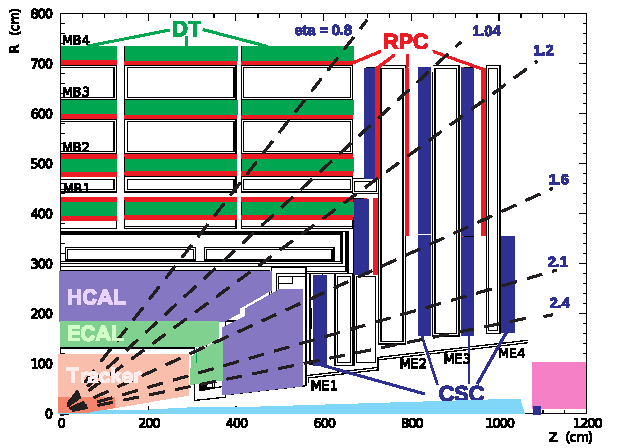
\includegraphics[width=0.8\textwidth]{plots/muonsys.pdf}
  \caption{Cross section of the CMS detector along the beam-pipe~\cite{muonid2}. The highlighted regions show the positioning of its muon system.}
  \label{fig:muonsys}
\end{figure}

The chambers are organized as wheels in the barrel region and disks in the endcap region. The three different types of gas based detectors cover an area of $25\,000\,\text{m}^2$. A wide angle coverage is also ensured by extending up to $|\eta| < 2.4$.

\subsubsection{Drift Tubes}
\label{sec:drift-tubes}

Drift Tubes (\textbf{DT}) are installed in the barrel region ($|\eta| < 1.3$) in between the iron return yoke plates. They operate well with a comparatively low muon rate and a fairly uniform magnetic field, which is contained by the iron yoke. The low cost is also beneficial, considering the large area ($172\,000$ tubes) that needs to be covered in this region. Overall there are four cylinders of muon chambers, usually called ``stations''. Every drift tube chamber consists of three superlayers, which contain four layers of drift cells. An exemplary cell is shown in figure~\ref{fig:drift-cell}.

\begin{figure}[!htb]
  \centering
  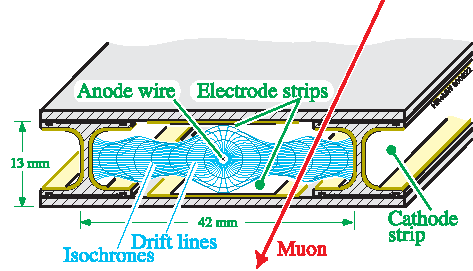
\includegraphics[width=0.5\textwidth]{plots/driftcell.pdf}  
  \caption{Schematic drift cell of the drift tubes in the muon system of the CMS detector~\cite{driftcell}. Both the driftlines and isochrones are shown.}
  \label{fig:drift-cell}
\end{figure}

In the first three stations, the cell in the middle is responsible for measuring the $z$-coordinate, while the other two measure the $r$-$\phi$-component. The fourth station is only equipped with two superslayers, which focus on the $r$-$\phi$ measurement. Each of the $2.4\,\text{m}$ long cells has a gold plated steel wire as an anode in the middle of the chamber with aluminium tape on each side of the wall acting as a cathode. As a muon crosses a cell, it ionizes the argon ($85\pct$), carbon dioxide ($15\pct$) mixture. The resulting electrons (ions) drift towards the anode (cathode), leading to a measurable current. While a single cell has a spatial resolution of $250\,\mu\text{m}$, one station with $2 \times 4$ hits reaches $100,\mu\text{m}$.

\subsubsection{Cathode Strip Chambers}

The endcap region is faced with much higher muon and background fluxes, along with an inhomogeneous magnetic field. As a consequence, cathode strip chambers (\textbf{CSC}) are the detector of choice instead of DTs. They cover the $|\eta|$ range from $0.9$ to $2.4$, overlapping slightly with the DTs. The CSCs are trapezoidally shaped and consist of seven layers of radially oriented cathode strips each. Anode wires are placed perpendicularly to the strips inside the gas filled ($40\pct\,\text{Ar} + 50\pct\,\text{CO}_2 + 10\pct\,\text{CF}_4$) gaps in between each layer. This layout allows for measuring both the $\phi$-component with the strips and the $r$-component with the wires at the same time. The spatial resolution varies between $75\,\mu\text{m}$ and $150\,\mu\text{m}$.

\subsubsection{Resistive Plate Chambers}

The third and final detector type are the resistive plate chambers (\textbf{RPC}). In comparison to the previous two components, they provide much faster response times due to being operated in avalanche mode. In the barrel region, there are overall six RPCs embedded. On the first two drift tube stations, there is one RPC mounted on each side, while only one is installed on each of the two outer stations. Additionally, there are planes of RPCs in between each of the first three stations of the endcaps region. This results in an overall coverage of $|\eta| < 1.6$, which will be expanded upon in the next upgrade cycle. The detector works with two parallel plates, where the gap is gas filled and read-out strips are placed in the middle. The usage of avalanche mode allows for response times comparable to scintillators, while the geometry yields adequate spatial resolution. \\

By combining the information from both the inner tracker, as well as the muon chambers, an overall resolution for transverse momentum of $5\pct$ for highly energetic particles ($\sim 1\,\text{TeV}$) can be reached.



\subsection{Triggering and Data Aquisition}

Upon reaching the design luminosity, there are collisions every $25\,\text{ns}$ corresponding to a rate of proton-proton interactions of about $10^9\,\text{Hz}$. However, the amount of data that is possible to be stored is roughly $10^2\,\text{Hz}$. Therefore a preselection, specifically choosing events that potentially contain relevant physics, has to be made. The amount of data to be stored per event is reduced to about $1\,\text{MB}$ in the process. The CMS experiment uses a two-level \textit{triggers} system to perform said reduction. \\

The \textbf{Level-1} (\textbf{L1}) trigger is mostly based upon programmable electronics, which make use of the information provided by the different sub-detectors. Figure~\ref{fig:lvl1trig} shows the information chain of the L1 trigger system. Local triggers collect the basic information from the detector components, which are then combined in regional triggers and are eventually transferred to the global trigger. The latter decides whether or not to discard the event, by performing a preliminary reconstruction. The maximal latency between a bunch crossing and distributing the conclusion to read out the electronics is $3.2\,\mu\text{s}$. Overall, the L1 rate of events to about $30\,\text{kHz}$ (design rate limit is $100\,\text{kHz}$; typically running at $98\,\text{kHz}$).

If an event is selected by the L1, the front-end buffers of all the sub-detectors are read out and the data is forwarded to the \textbf{data aquisition} (\textbf{DAQ}) system. Here the \textbf{high level trigger} (\textbf{HLT}) performs a much more sophisticated analysis on the collected data. It is able to do so, because it can access all digitized information. This provides an additional reduction to about $2\,\text{kHz}$ (original design rate was $300\,\text{Hz}$).

Distributing the analysed data is the next step. The processed datasets are transferred from the Tier-0 at CERN to the Tier-1 locations, where further analyses are run. Next, it is distributed to the final destination in regards to central storage, the Tier-2 data centers. All CMS workgroups can access the datasets at this stage. It should be noted that the Tier-1 computing grid is also used for large-scale analyses, while the Tier-2 resources are used for regular analyses.


\begin{figure}[ht!]
  \centering
  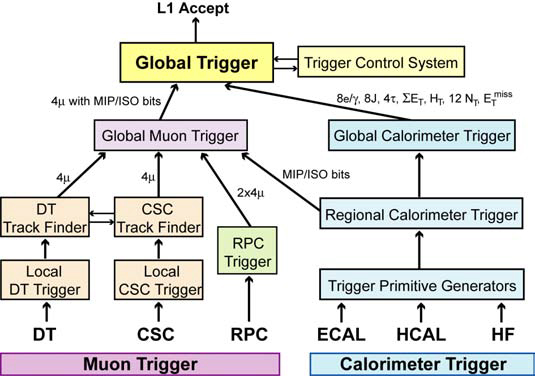
\includegraphics[width=0.55\textwidth]{plots/lvl1trigger.jpg}
  \caption{Schematic overview of the architecture of the Level-1 trigger of the CMS experiment~\cite{cmsjinst}.}
  \label{fig:lvl1trig}
\end{figure}


\subsection{Object Reconstruction}
\label{sec:objreco}

The information provided by the respective sub-detectors, such as a chamber hit or an energy deposit, have to be combined to a physics object for further analysis. Different kinds of objects have individual algorithms. The ones relevant for the analysis will be covered in the next sections. \\

The reconstruction of \textbf{Muons} is solely based on their trajectory. Initially the tracker and muon system hit information are reconstructed separately. If a muon is reconstructed in the muon system, it is considered a \textit{standalone muon}. The Kalman filtering technique~\cite{kalman} is used to create a trajectory. Starting with a seed, it considers nearby hits to iteratively build the track. Progressing on from the initial standalone muon track, one can compare it to a tracker trajectory by propagating both their parameters to a common plane. If a matching set of hits can be found, the muon becomes a \textit{global muon} which is the most commonly used quantity. Alternatively the initial track can be taken from the tracker. These muon candidate trajectories are then extrapolated by taking various factors like average energy depositions, multiple scattering, precise magnetic field maps or Bremsstrahlung into account. If matching track segments are found in the muon system, the muon becomes a \textit{tracker muon}. The latter is particularly useful for multiple (usually two) collimated muon tracks, as the spatial resolution of the tracker exceeds the one of the muon system by far. \\

\textbf{Jets} are a conglomerate of various, mostly hadronic particles. They usually stem from either a gluon or a quark. As jets are reconstructed as a single object, a specific algorithm has to be chosen to perform this task. A popular choice are sequential recombination algorithms such as the Cambridge/Aachen algorithm. In this analysis the \textbf{anti-$k_\textbf{T}$} clustering algorithm~\cite{antikt} will be used. It is both collinear and infrared safe, meaning that the reconstruction is neither significantly affected by splitting in the collinear direction nor the emission of soft particles. Unlike the other sequential recombination algorithms, this method provides a conical shape for which the cone radius parameter will be set to $R = 0.5$.

Both \textbf{electrons} and \textbf{photons} are mainly measured via the ECAL~\cite{elereco}. While the electron radiates photons as its trajectory is bent by the magnetic field, photons with sufficient energy can lead to pair production under the influence of electromagnetic fields. In combination, this leads to an electromagnetic shower, which covers a cluster of roughly $5 \times 5$ ECAL cells for particles of intermediate energies. Measuring this shower allows for estimation of the energy of the initial particle. An additional transverse momentum measurement from the tracker is also possible for tracks of charged particles. Building these is initiated by superclusters (clusters of clusters) in the pixel detector and uses a Gaussian Sum Filter with a specific energy loss model.

While photons do initially not carry any charge, they tend to produce electron-positron pairs when under the influence of an atom's electric field. Electrons also radiate photons as they are subject to the Coulomb field of a nucleus, which are then again able to lead to pair production. As such, both types of objects produce a particle track until their energy has decreased sufficiently that they can be absorbed into the detector material.

\textbf{Missing transverse energy} is calculated from the vectorial sum of the transverse energies of all reconstructed objects. As one expects the initial state of a proton-proton collision to only have a negligible amount of transverse energy, the aforementioned sum should be zero. However, certain particles such as neutrinos or possibly new, yet unknown ones can escape the detector. The negative value of the vectorial sum is the collective estimate for all particles that avoided detection.

While most reconstruction algorithms work independently from one another to identify particle candidates, the \textbf{particle-flow} algorithm~\cite{pflow} reconstructs entire events. This effectively means, that the tracks of every muon, electron, photon, as well as the charged and neutral hadrons are being taken into account when identifying particles. Consequently it is necessary to consider all sub-detectors and the information they provide. Overall, the expected performance for accurately identifying and reconstructing jets, taus and missing transverse energy is improved. Taking jets as an example, the components each jet consists of are reconstructed individually. Instead of approximating the shape through a cone, even the low energy fragments with diverging tracks can be assigned to the right jets. Taking all the information (that the algorithm considers) about nearby particles into account, an in-depth isolation criterion can be defined. This is particularly useful for muons used in this analysis.



%%% Local Variables: 
%%% mode: latex
%%% TeX-master: "document"
%%% End: 


% analysis
\chapter{Signature of the Signal}
\label{cha:sig}

As discussed in section~\ref{sec:anamodel}, the model used in the analysis is $R$-parity violating supersymmetry. In particular, single coupling dominance for the lepton number violating coupling $\lambda^\prime_{211}$ is assumed. With a two quark initial state, the production of sleptons inevitably dominates other constellations. Considering how low values for the couplings have to be (Cf.~fig.~\ref{fig:auterrpv}~\&~\ref{fig:2011rpv}), the primary decay modes for the slepton will be the $R$-parity \textit{conserving} $\nu + \tilde{\chi}$ or $\mu + \tilde{\chi}$ combination. The $R$-parity \textit{violating} dijet channel can be neglected as it will be both rare and overshadowed by standard model processes. The lightest neutralino is assumed to be the lightest supersymmetric particle (\textbf{LSP}) in this analysis. As a result the decay products of both the neutralino and chargino can lead to additional jets or leptons, but will eventually lead to the lightest neutralino through $R$-parity conserving modes\footnote{The details of the decay modes depend on the mass hierarchy determined by the RPV cMSSM model parameters} (Fig.~\ref{fig:resosmusneu}). 


\begin{figure}[ht!]
  \centering
  \begin{subfigure}[b]{0.495\textwidth}
    \centering
    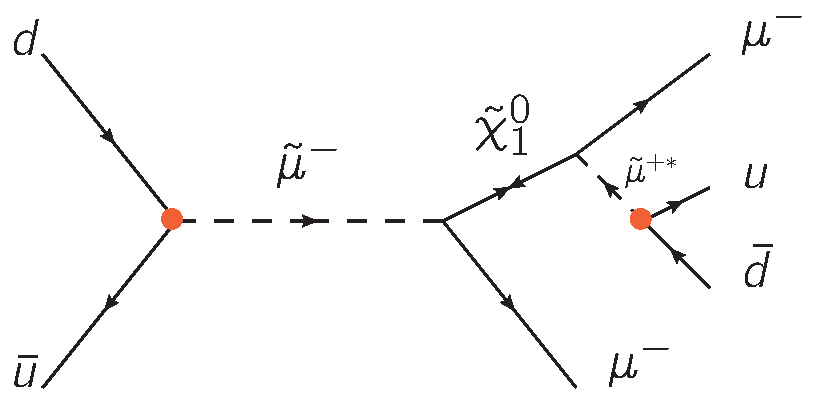
\includegraphics[width=\textwidth]{plots/rpv-resonant-smuon-samesign-mumuqq.pdf}
    \caption{\label{fig:ressmu}}
  \end{subfigure}
  \begin{subfigure}[b]{0.495\textwidth}
    \centering
    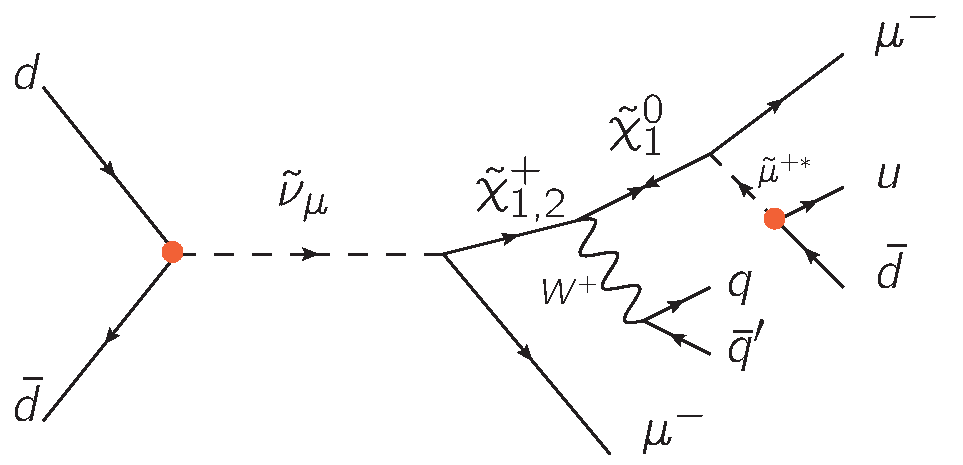
\includegraphics[width=\textwidth]{plots/rpv-resonant-sneutrino-chargino-mumuqq.pdf}
    \caption{\label{fig:ressneu}}
  \end{subfigure}
  \caption{Resonant production of a smuon~(\ref{fig:ressmu}) and a sneutrino~(\ref{fig:ressneu}) in $R$-parity violating supersymmetry. Shown are the most simple Feynman graphs leading to the two muon, two jets final state. The lepton number violating vertices are marked in red.}
  \label{fig:resosmusneu}
\end{figure}


Since it is the LSP, it can only decay through the $\lambda^\prime_{211}$ coupling via a virtual smuon or sneutrino. It should also be noted that the lifetime of the LSP depends on the coupling strength. For values $\lambda^\prime_{211} > 10^{-6}$, the decay will be perceived as ``prompt'' by the detector. This means that both muons should originate from the same (primary) vertex. The decay of the LSP subsequently adds two jets, as well as either a muon or neutrino. With missing transverse energy from neutrinos being significantly less attractive than muon signatures, these final states are neglected. 


This leaves two jets and a number of muons, ranging from zero to two, in every decay. Considering the production rates for the relevant backgrounds, one can see that two compositions are disfavoured. Colliding two hadrons yields a high amount of jets in every event, making the pure dijet channel without any muon the least promising. The very high $W + \text{jets}$ background would interfere with a single muon with two jet search, leaving only the two muons, two jets option. Even here there are significant backgrounds to tackle, primarily the Drell-Yan process.

Taking a look at the simplest Feynman graphs for resonant smuon and sneutrino production and decay at the LHC (Fig.~\ref{fig:resosmusneu}), one will notice a very useful attribute of their decay products. The electric charge of both muons are equally as likely to have the same sign as the opposite sign. This is due to the neutralino being a Majorana particle. Keeping the initial state of two protons in mind, primarily the ratio of $u$ to $d$-quarks, the likelihood of positively charged muons is roughly twice the one for negatively charged ones. Since most Standard Model backgrounds are able to produce two opposite, but not two same sign muons, this feature of RPV supersymmetry can be exploited to discriminate against them. Major backgrounds, such as the aforementioned Drell-Yan processes or the production of top quark pairs, can be greatly reduced, enabling searches for new physics with low cross sections.


\section{Monte Carlo Study}
\label{sec:mcstudy}

As Monte Carlo (\textbf{MC}) simulations are used for comparison to the measured data, the simulation of the signal for the 2011 analysis~\cite{2011rpv} can be used to derive further information about the signature. The production process of such a simulation will be outlined in an upcoming section (Sec.~\ref{sec:signal-sim}). Using the RPV supersymmetry model explained in section~\ref{sec:anamodel}, a grid of simulated signal points with $50\,\text{k}$ events each has been generated. While the mass of the scalar sparticles $m_0$ runs from $100$ to $2000\,\text{GeV}$ in steps of $100\,\text{GeV}$ and the mass of fermionic sparticles runs from $50$ to $1000\,\text{GeV}$ in steps of $50\,\text{GeV}$, the remaining model parameters have the following fixed values:

\begin{equation*}
  A_0 = 0, \quad \tan{\beta} = 20, \quad \text{sgn}\,\mu = +1, \quad \lambda^\prime_{211} = 0.01
\end{equation*}

While the cMSSM parameter values are inspired by the low mass benchmark points of CMS~\cite{cmssusybenchmarkpoints}, the have a low impact on the relevant processes. The value of $\lambda^\prime_{211}$ is based on a roughly estimated sensitivity for hadron colliders~\cite{rpvimpl}. Because certain regions (low $m_{1/2}$, high $m_0$) in this parameter space lead to unphysical phenomena such as non-converging renormalization group equations, tachyonic solutions or no electroweak symmetry breaking, they are not being simulated. Excluding these points in the grid leaves an overall amount of $354$ simulated phase space points (Cf.~fig.~\ref{fig:sigeff}). \\

Various decay scenarios are being investigated in this grid to determine their respective contribution to the signal signature. Two cases are considered. In the first one at least two muons and two jets are required (\textbf{MU2J2}). This yields signal events, but not all of them pass all analysis requirements. Only the second one demands all analysis requirements (from 2011~\cite{2011rpv}) to be met (\textbf{ANA}). Major differences between the two are the same sign charge requirement and isolation criteria for muons. While it is important to know that the latter is tighter than the first, the details of all the requirements will be discussed in-depth in the event selection\footnote{Although the event selection will concern itself with the 2012 requirements, they are comparable to the ones used in 2011.} (Cha.~\ref{cha:eventsel}). Comparing both types of cases gives an idea of the effect of the analysis requirements on the signal.

To determine the overall efficiency of selecting signal events, only the MU2J2 and ANA cases without any specific decay scenario are shown in figure~\ref{fig:sigeff}.

\begin{figure}[ht!]
  \centering
  \begin{subfigure}[b]{0.495\textwidth}
    \centering
    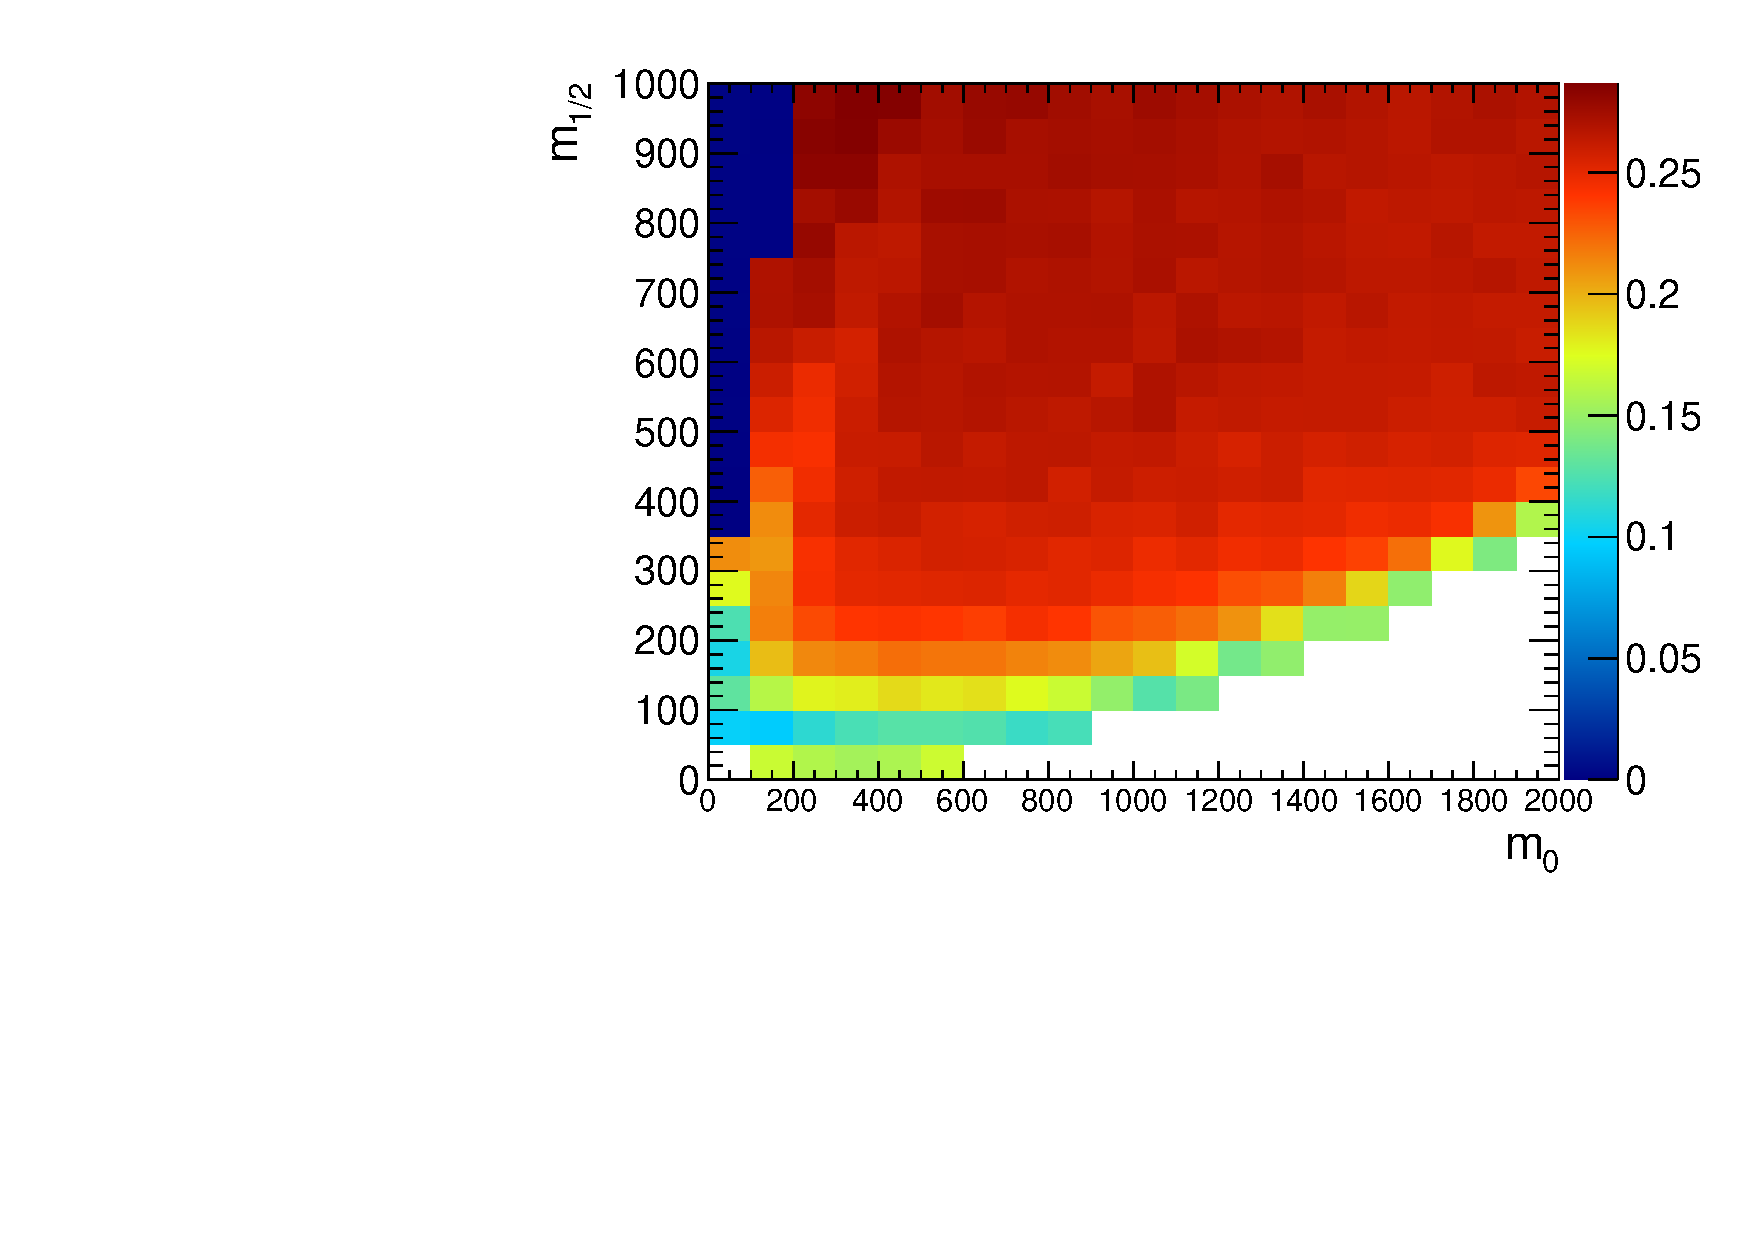
\includegraphics[width=\textwidth]{plots/hSignalRatio.pdf}
    \caption{\label{fig:sig}}
  \end{subfigure}
  \begin{subfigure}[b]{0.495\textwidth}
    \centering
    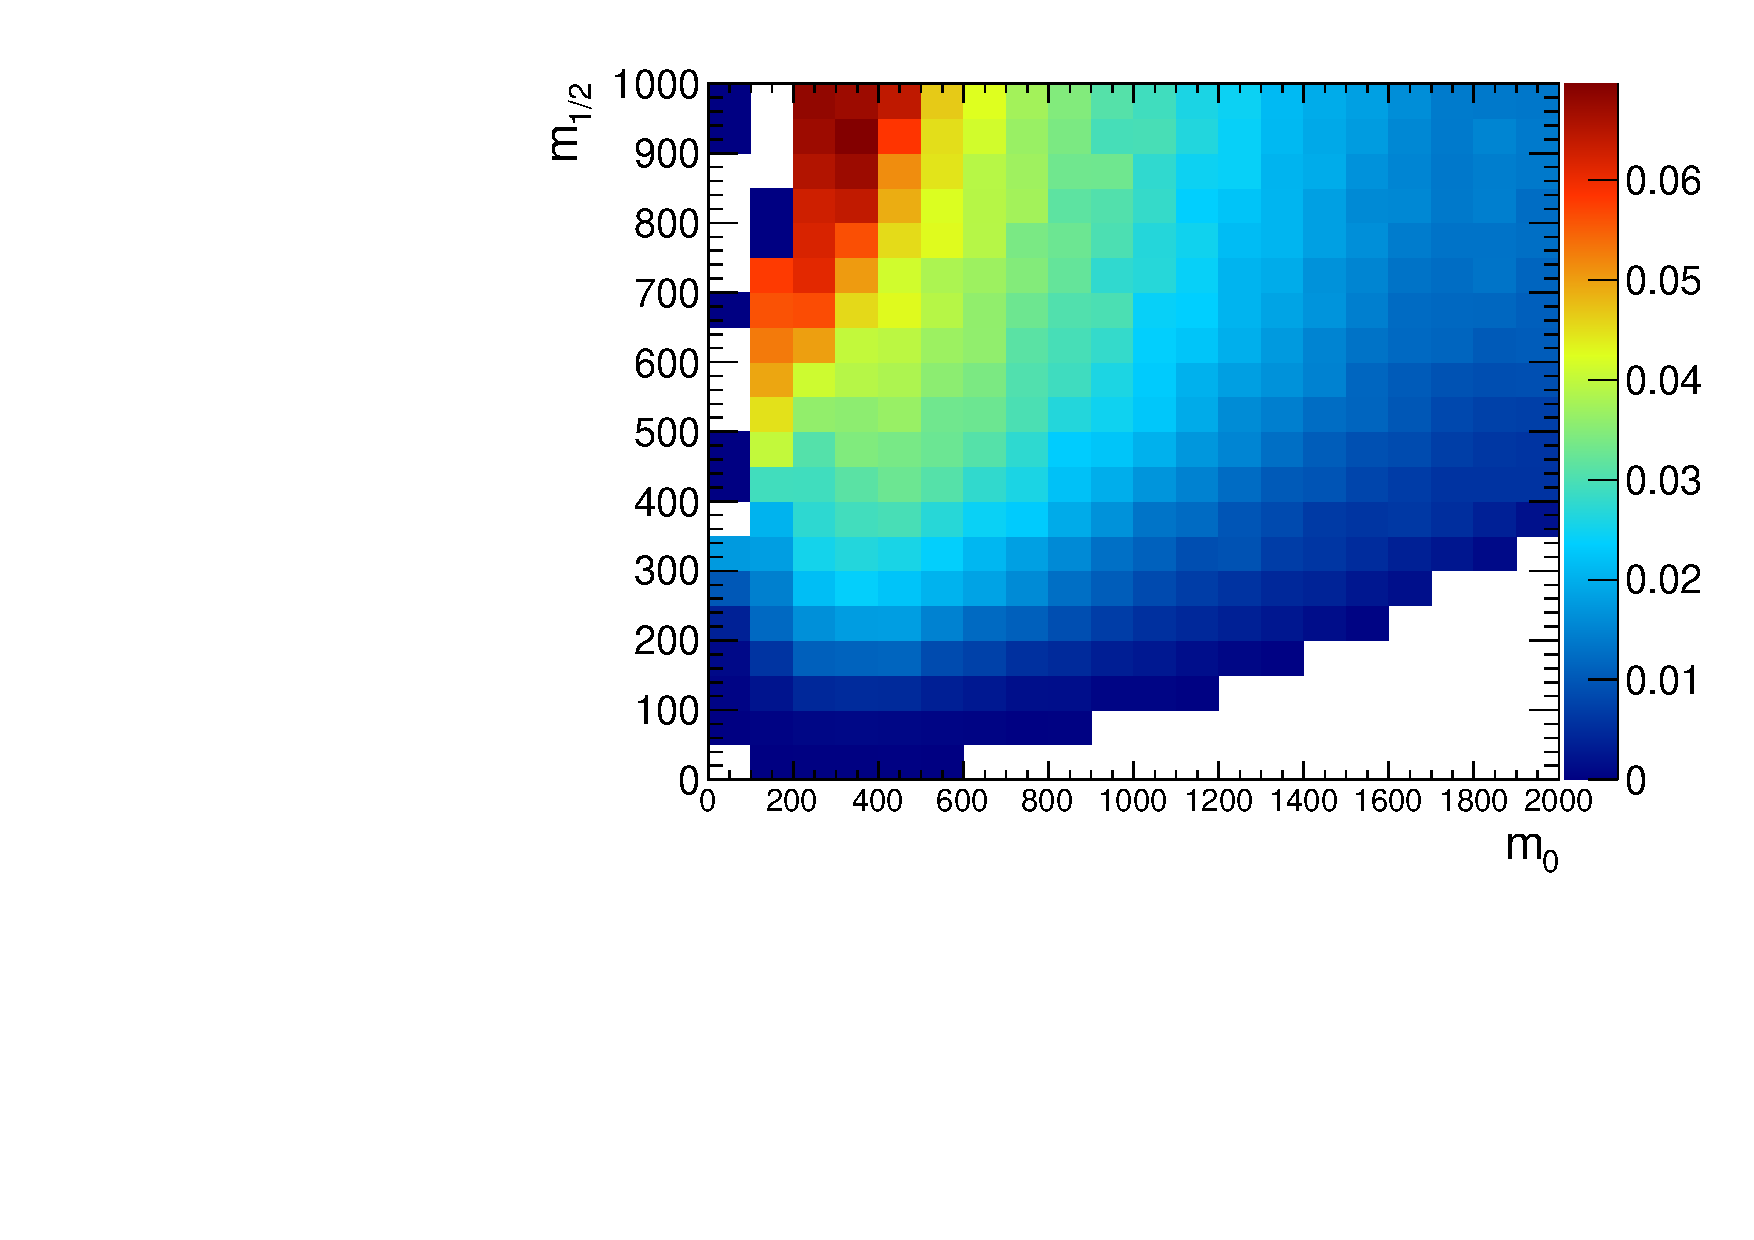
\includegraphics[width=\textwidth]{plots/hCutSignalRatio.pdf}
    \caption{\label{fig:cutsig}}
  \end{subfigure}
  \caption{Efficiency of selecting signal events in the MU2J2~(\ref{fig:sig}) and the ANA case~(\ref{fig:cutsig}). Each bin represents a Monte-Carlo simulation of a RPV supersymmetry point normalized to the generated number of events.}
  \label{fig:sigeff}
\end{figure}

\noindent Each bin shows the number of events meeting the requirements, normalized to the generated number of events. The white bins contain no events. This is either because no events passed the requirements, or they are within the previously mentioned low $m_{1/2}$, high $m_0$ parameter region with unphysical results. For high $m_{1/2}$, but low $m_0$ there are also disproportionally few events. The reason for this disparity lies within the supersymmetric mass spectrum. The lightest supersymmetric particle changes from the lightest neutralino to the stau $\tilde{\tau}$. As a result, the decay chains are altered, therefore rendering the analysis requirements insensitive. 

Shifting the focus on the shape of the distribution, one will notice an almost flat efficiency of around $25\,\pct$ above a certain ratio of $m_{1/2}$ to $m_0$ in the MU2J2 case. However, adding the ANA requirements leads to an efficiency decline from the $\sim 6\,\pct$ high $m_{1/2}$, low $m_0$ region to either around or below $1\,\pct$ for increasing $m_0$ and $m_{1/2}$, respectively. A significant portion of the drop in efficiency is expected when using the ANA case. As discussed in the previous section, the additional same sign charge requirement will half the selected amount of events already. Any further requirements will also have a negative impact on the efficiency, with the isolation criteria for the two muons being the main cause for the decline. If the neutralino masses are much lower than the smuon mass, which is directly related to the universal mass parameters, it will naturally lead to boosted particles in the decay. Should these decay products be too collimated, the isolation criteria will not be met and the event will be discarded. It should be noted that, as a result of different branching ratios in certain phase space regions, different processes can dominate the final state. Consequently the requirements of the ANA case cannot impact the entire phase space equally. Therefore the origin of the decline is always a composite of multiple quantities. \\

By demanding certain amounts of specific particles in a decay chain, it is possible to reconstruct the process of a selected event. This type of demand will be referred to as an \textit{effective branching ratio} (\textbf{EBR})\footnote{Strictly speaking, these are not branching ratios, as it is a combination of multiple branching ratios and also depends on the production cross section.} To get an overview of the composition of processes leading to the signal signature, the particle count has been varied systematically. To reduce redundancy, only the primary produced sparticle as well as its supersymmetric decay products are used for process identification. Upon reaching the neutralino LSP in the cascade, the decay through the $\lambda^\prime_{211}$ coupling is always identical.

\begin{figure}[ht!]
  \centering
  \begin{subfigure}[b]{0.495\textwidth}
    \centering
    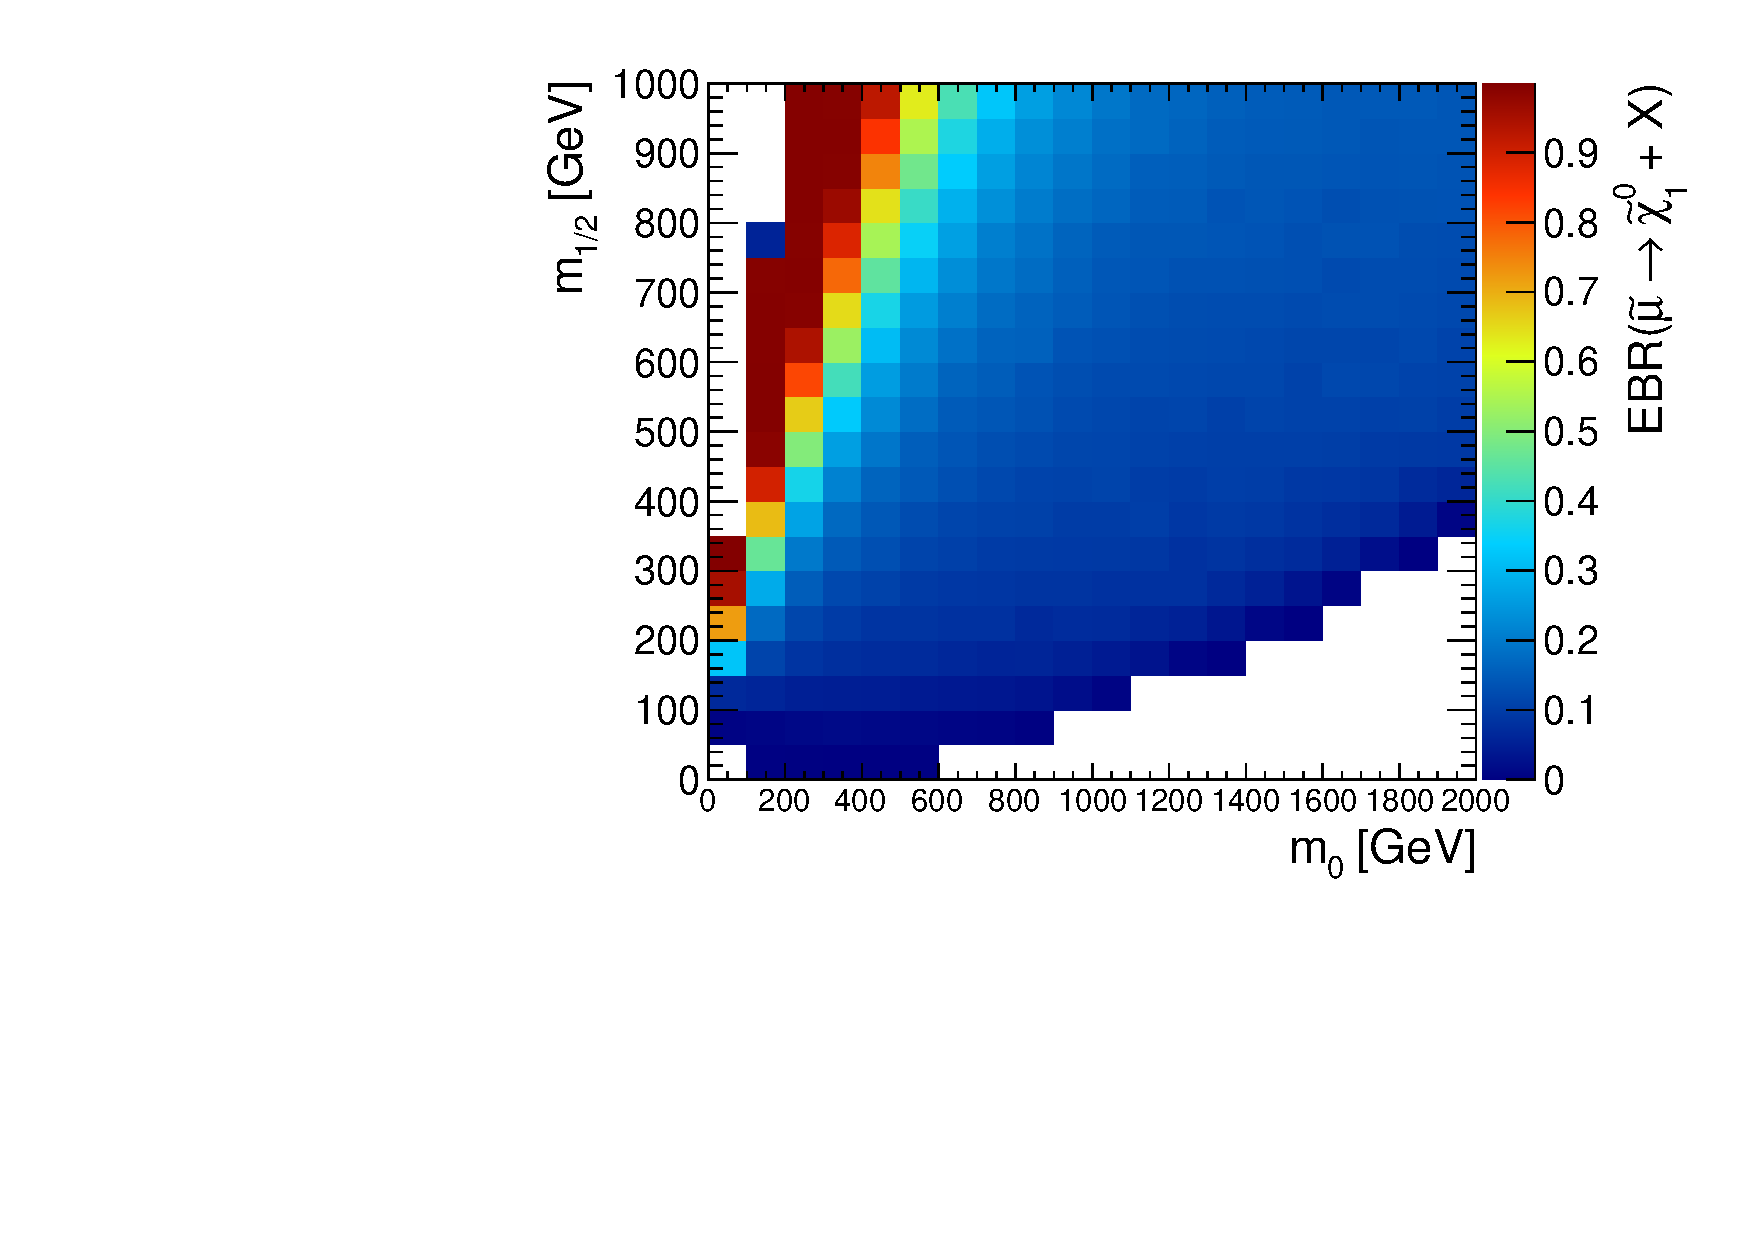
\includegraphics[width=\textwidth]{plots/hX01Ratio.pdf}
    \caption{\label{fig:x01}}
  \end{subfigure}
  \begin{subfigure}[b]{0.495\textwidth}
    \centering
    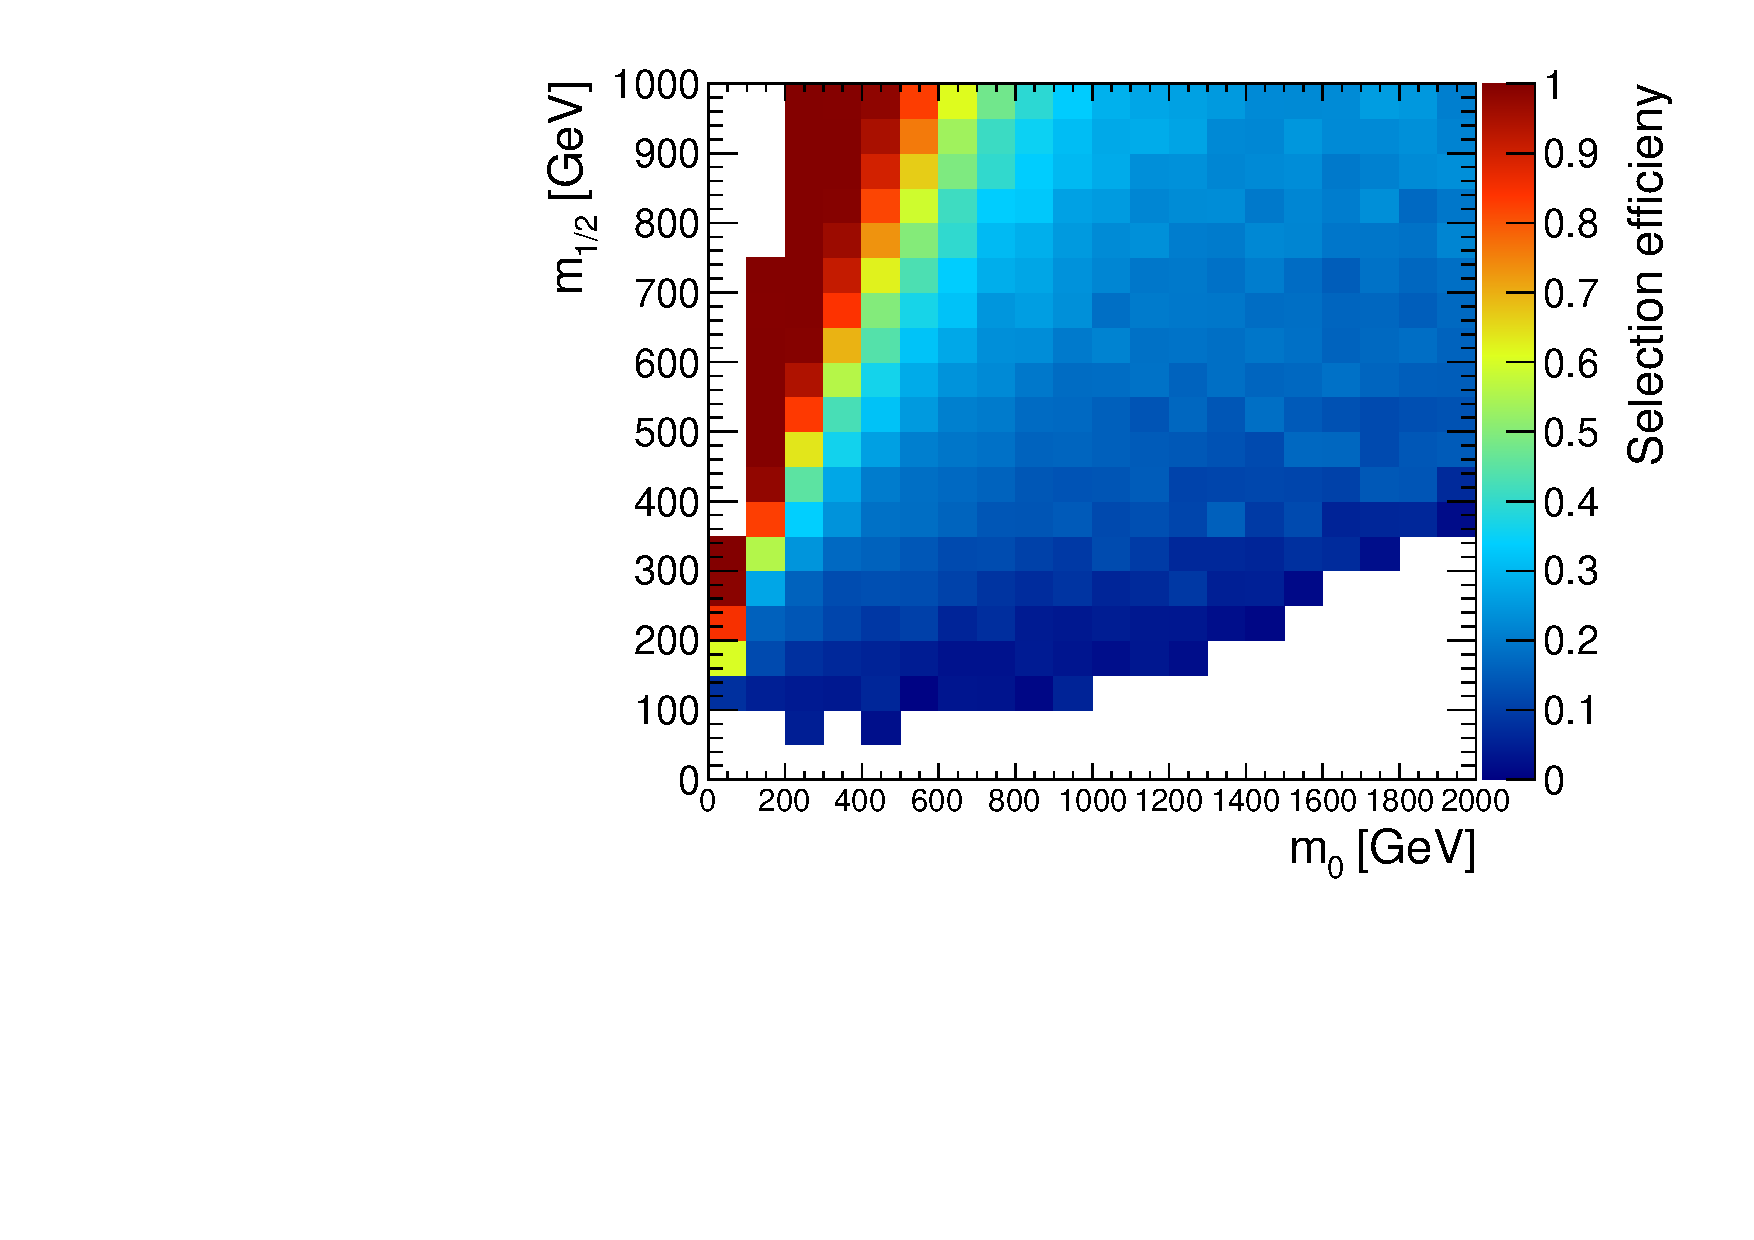
\includegraphics[width=\textwidth]{plots/hCutX01Ratio.pdf}
    \caption{\label{fig:cutx01}}
  \end{subfigure}

  \begin{subfigure}[b]{0.495\textwidth}
    \centering
    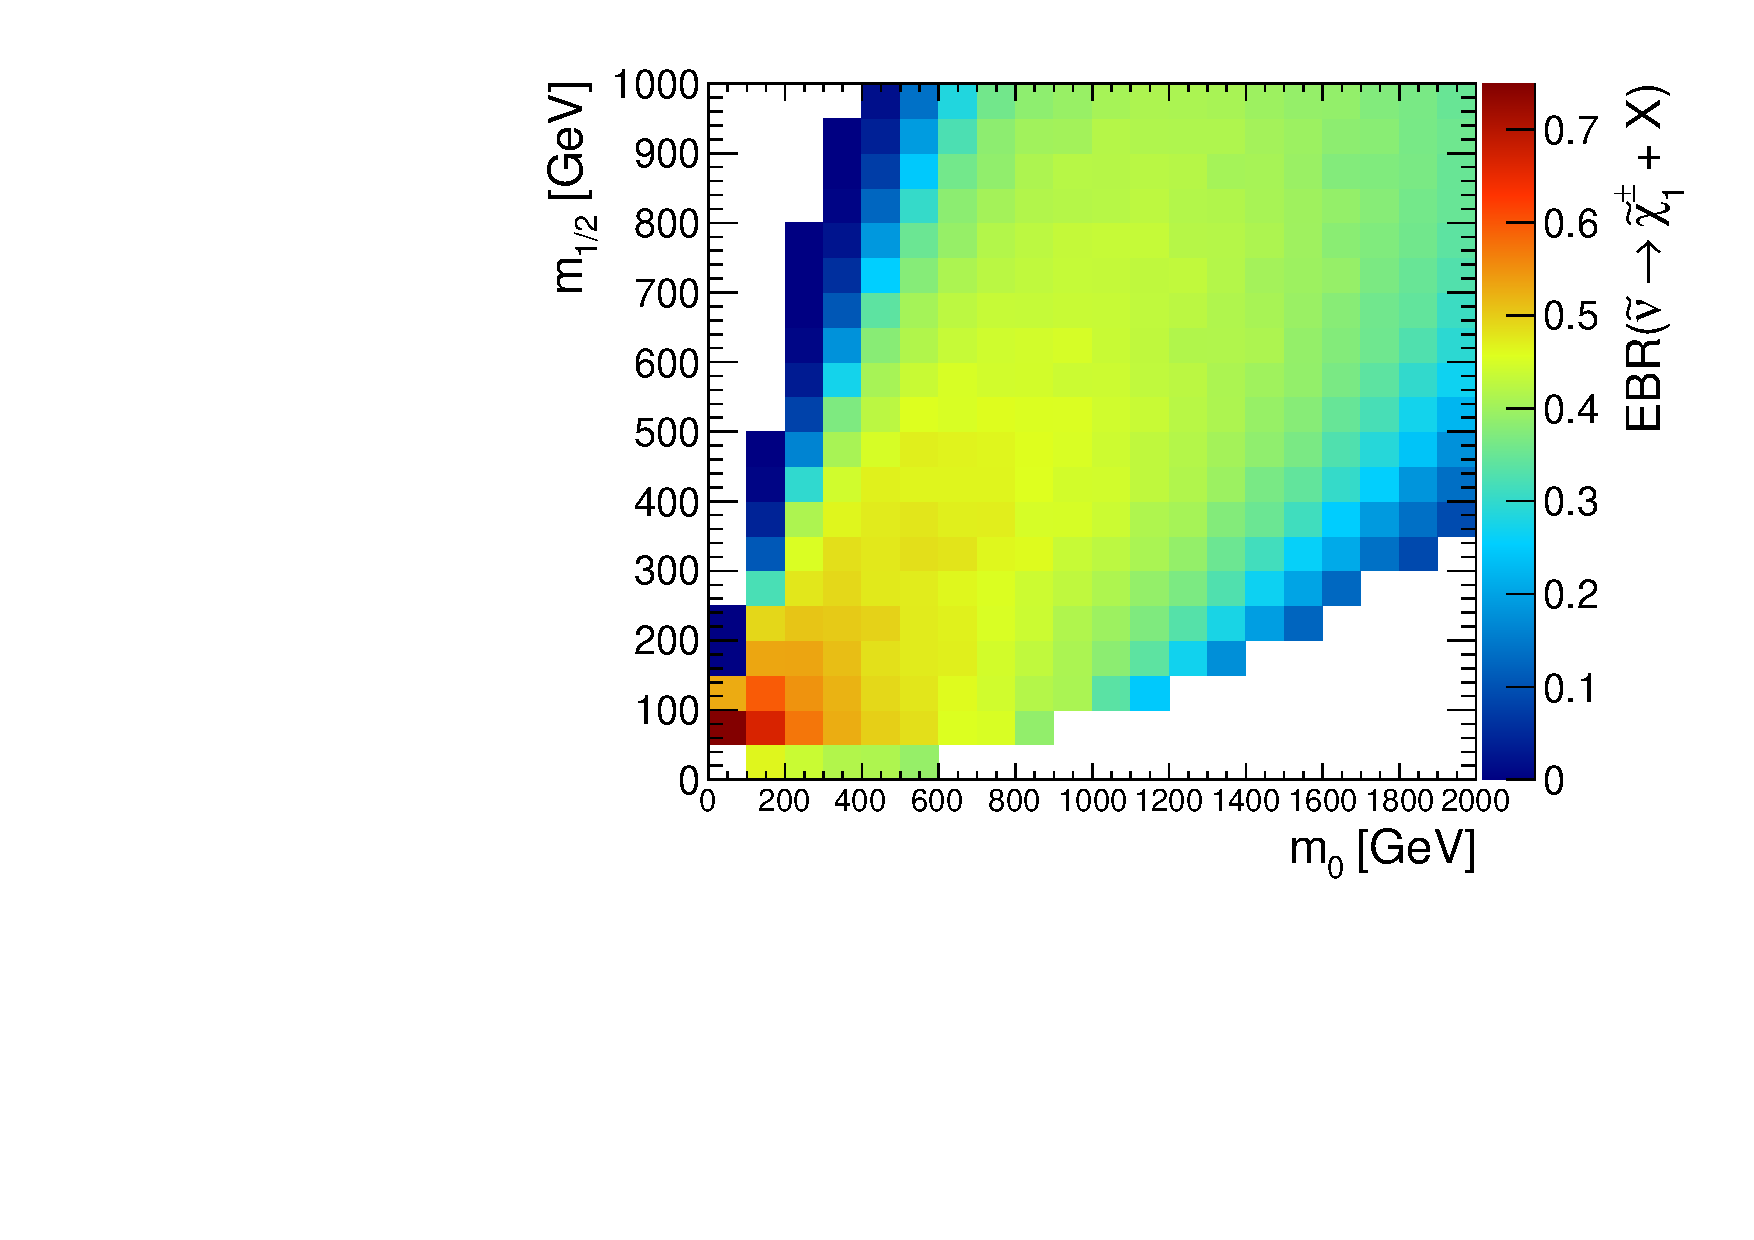
\includegraphics[width=\textwidth]{plots/hXplus1NeutRatio.pdf}
    \caption{\label{fig:xplus1neut}}
  \end{subfigure}
  \begin{subfigure}[b]{0.495\textwidth}
    \centering
    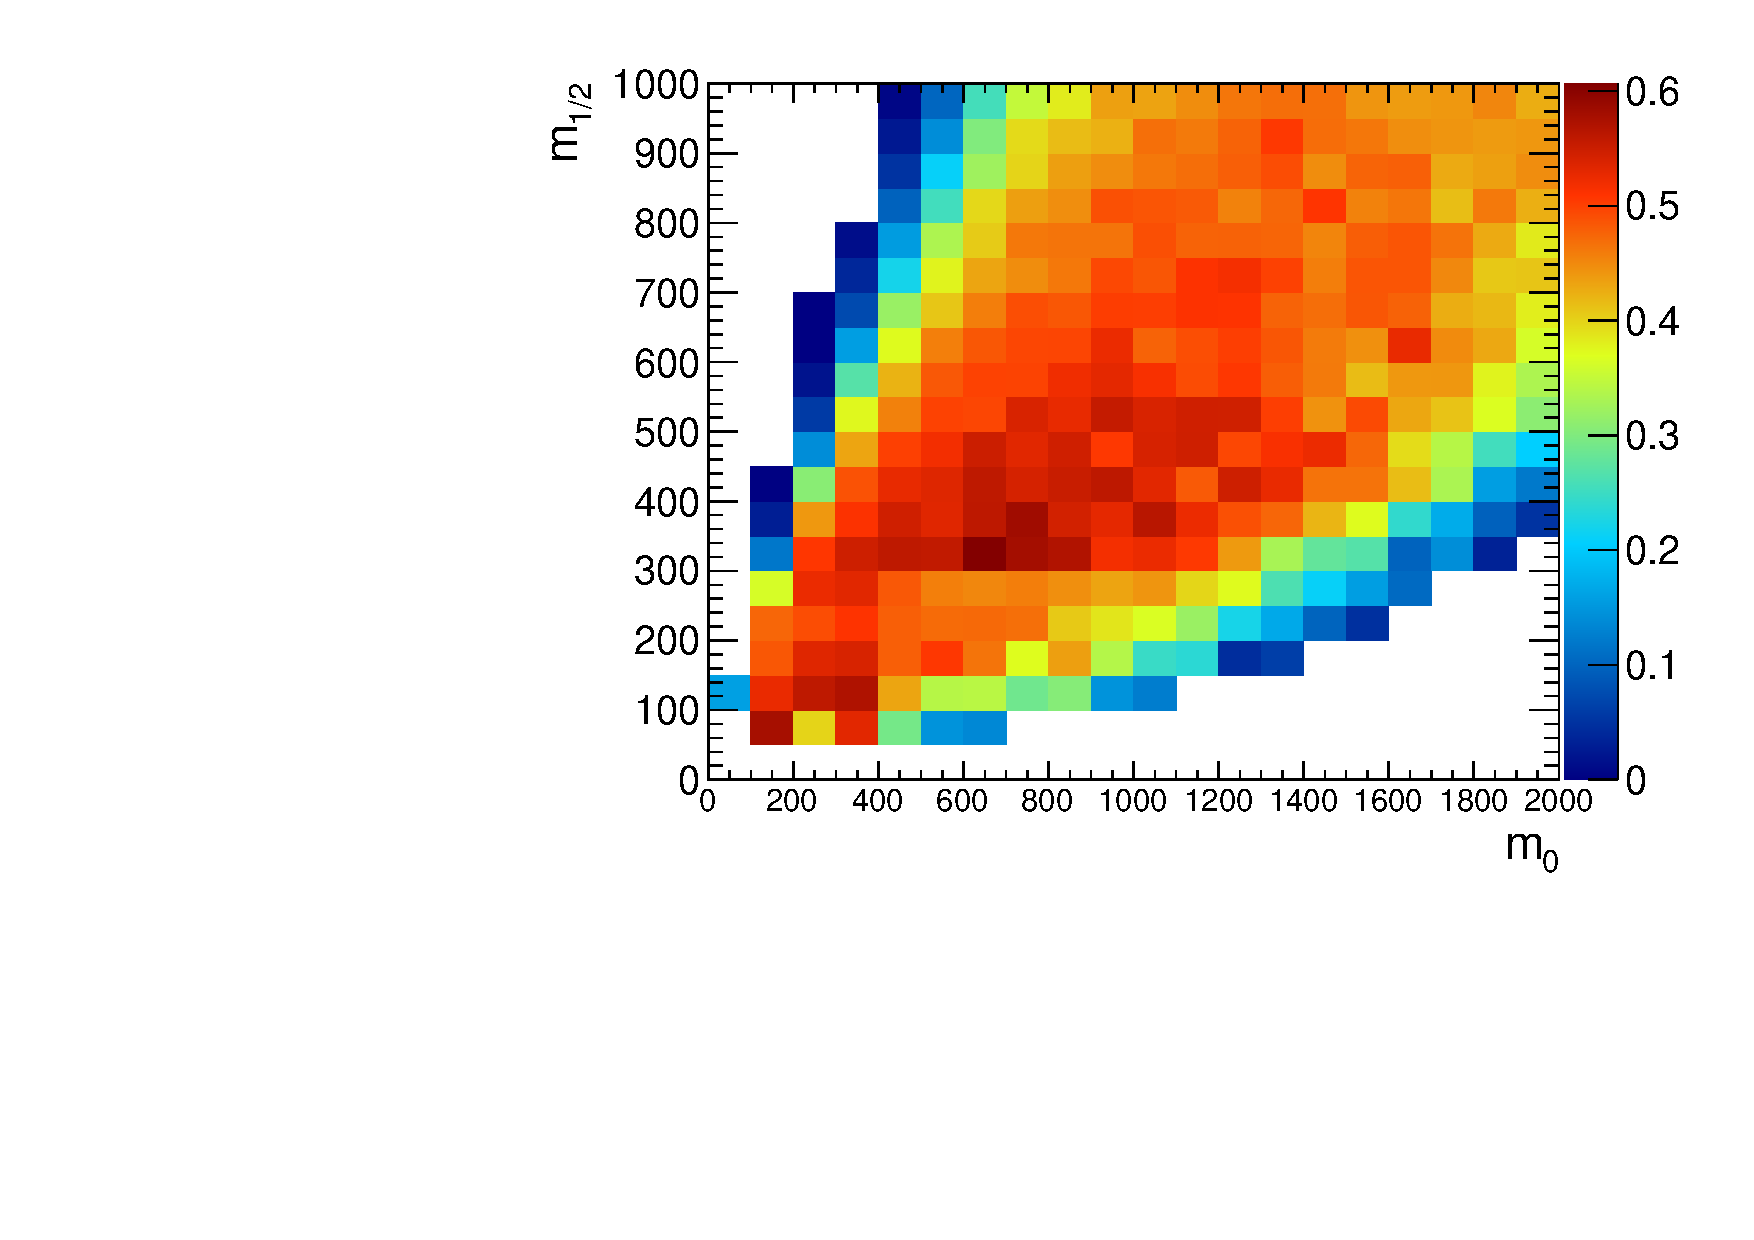
\includegraphics[width=\textwidth]{plots/hCutXplus1NeutRatio.pdf}
    \caption{\label{fig:cutxplus1neut}}
  \end{subfigure}
  \caption{Effective branching ratios of the $\tilde{\mu} \rightarrow \tilde{\chi}^0_1 + X$~(\ref{fig:x01}~\&~\ref{fig:cutx01}) and $\tilde{\nu} \rightarrow \tilde{\chi}^\pm_1 + X$~(\ref{fig:xplus1neut}~\&~\ref{fig:cutxplus1neut}) processes. The EBRs are given by $N_{\text{evt}}(\text{Events including decay products of process}) / N_{\text{evt}}(\text{All events for that bin})$ for each bin of the distribution in figure~\ref{fig:sigeff}. On the left the ANA case is shown, while one can see the MU2J2 case on the right.}
  \label{fig:x01sneuxplusratio}
\end{figure}

\noindent As an example, figure~\ref{fig:x01sneuxplusratio} displays the contributions to the overall selection efficiency from figure~\ref{fig:sigeff} of the $\tilde{\mu} \rightarrow \tilde{\chi}^0_1 + X$ and $\tilde{\nu} \rightarrow \tilde{\chi}^\pm_1 + X$ processes. The effective branching ratio is given by $N_{\text{evt}}(\text{Events including decay products of process}) / N_{\text{evt}}(\text{All events for that bin})$ for the individual bins of the overall selection efficiency.

Combining the ERBs for these two processes already covers roughly $50\pct$ for most of the parameter space. An efficient way to compare all relevant processes at once, is a one dimensional distribution with either of the two universal mass parameters set to a fixed value. Since a larger variation can be observed over the simulated $m_0$ range (Cf. fig.~\ref{fig:sigeff}~\&~\ref{fig:x01sneuxplusratio}), $m_{1/2}$ is kept constant.

\begin{figure}[ht!]
  \centering
  \begin{subfigure}[b]{0.495\textwidth}
    \centering
    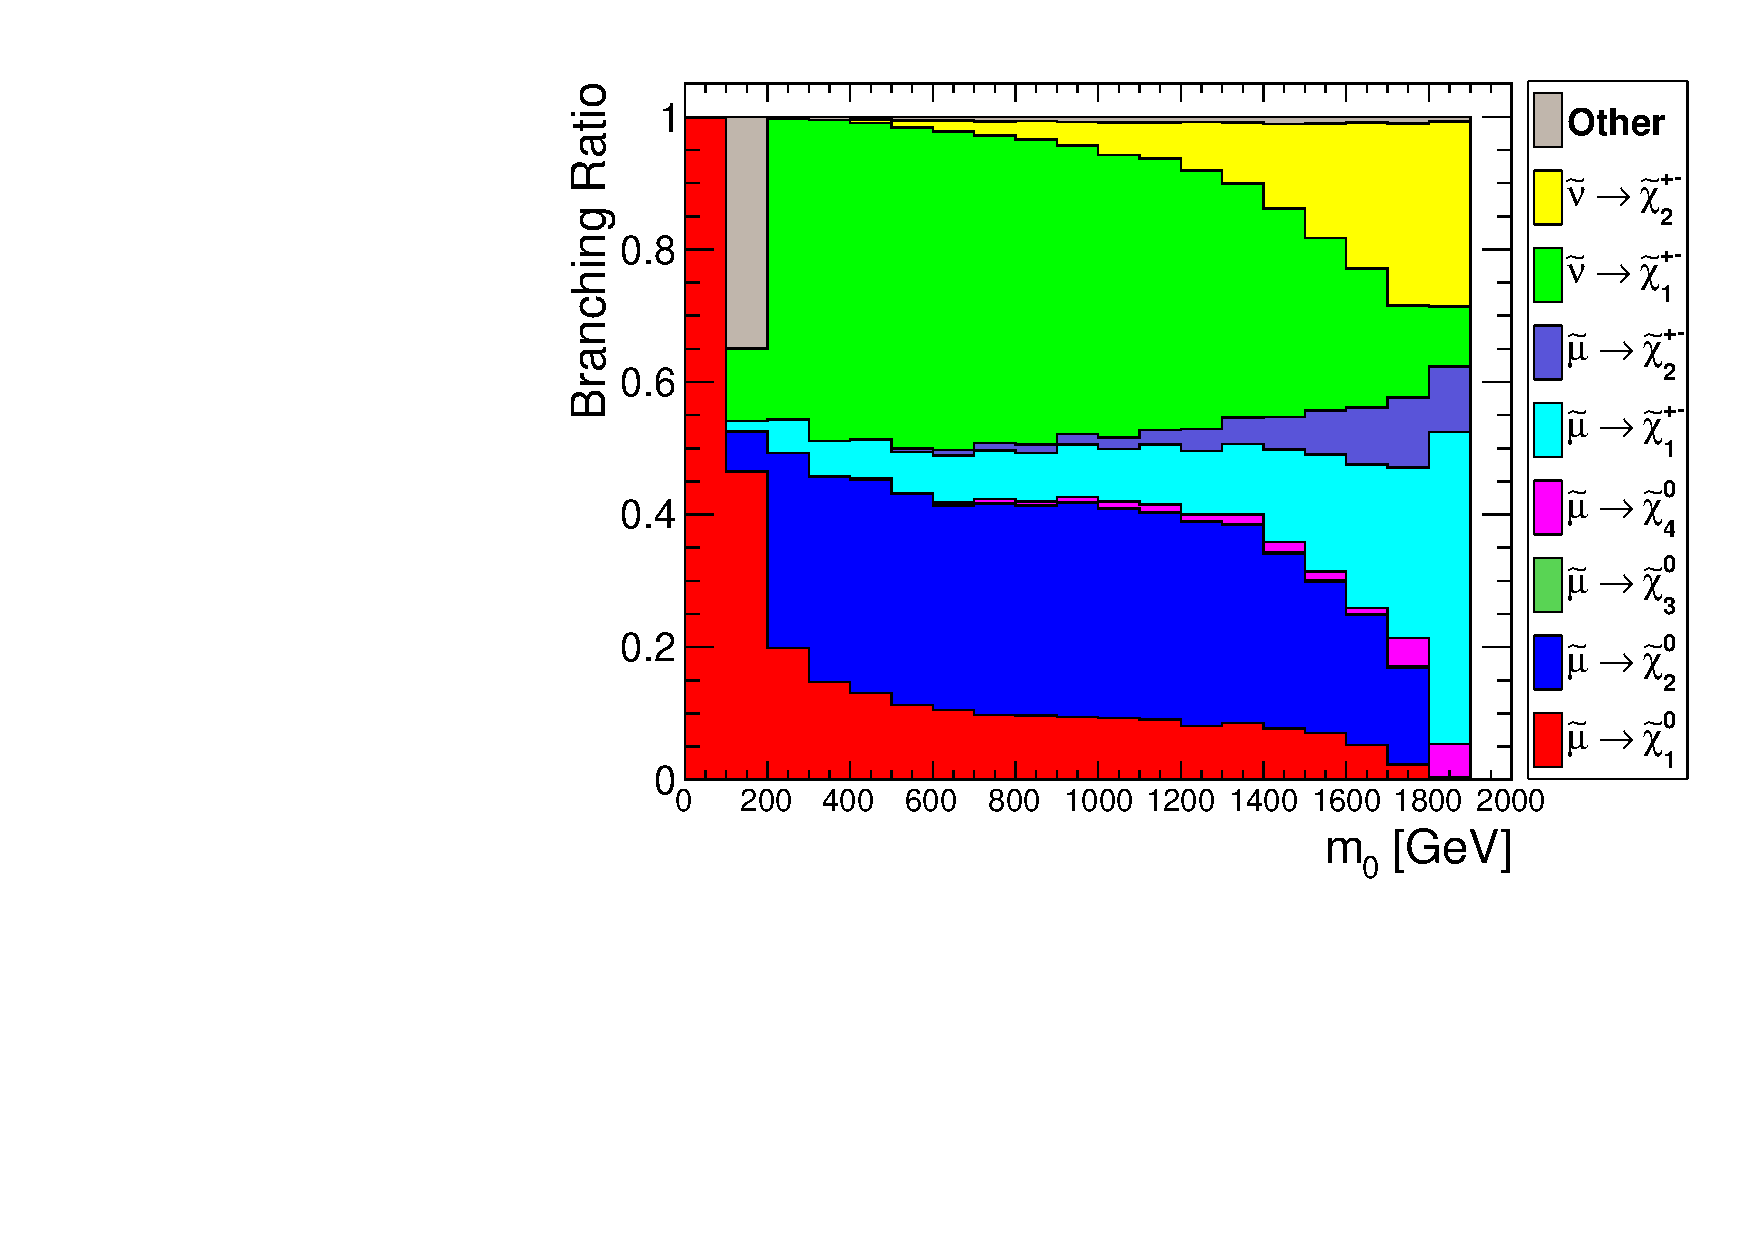
\includegraphics[width=\textwidth]{plots/hCrossRatio350.pdf}
    \caption{$m_{1/2} = 350\,\text{GeV}$\label{fig:crossratio350}}
  \end{subfigure}
  \begin{subfigure}[b]{0.495\textwidth}
    \centering
    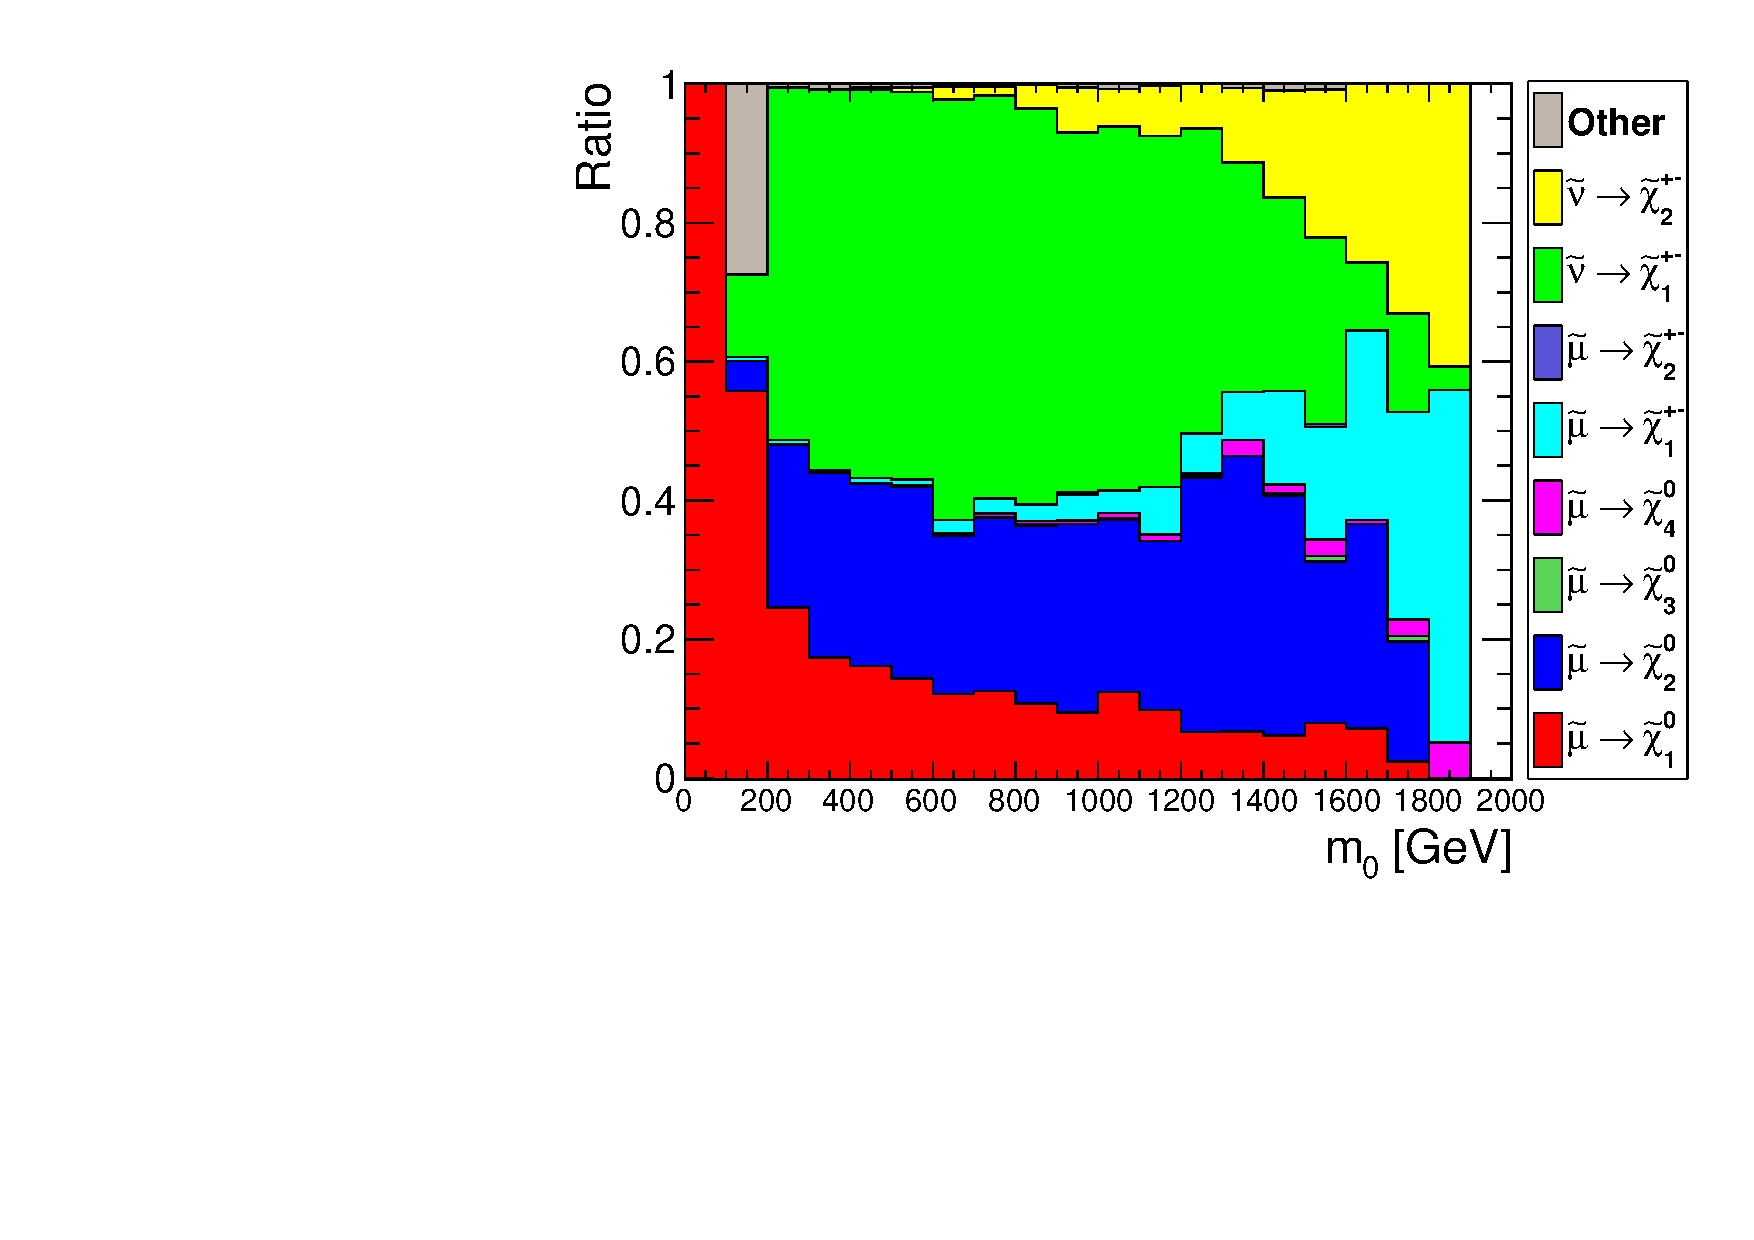
\includegraphics[width=\textwidth]{plots/hCutCrossRatio350.pdf}
    \caption{$m_{1/2} = 350\,\text{GeV}$\label{fig:cutcrossratio350}}
  \end{subfigure}

  \begin{subfigure}[b]{0.495\textwidth}
    \centering
    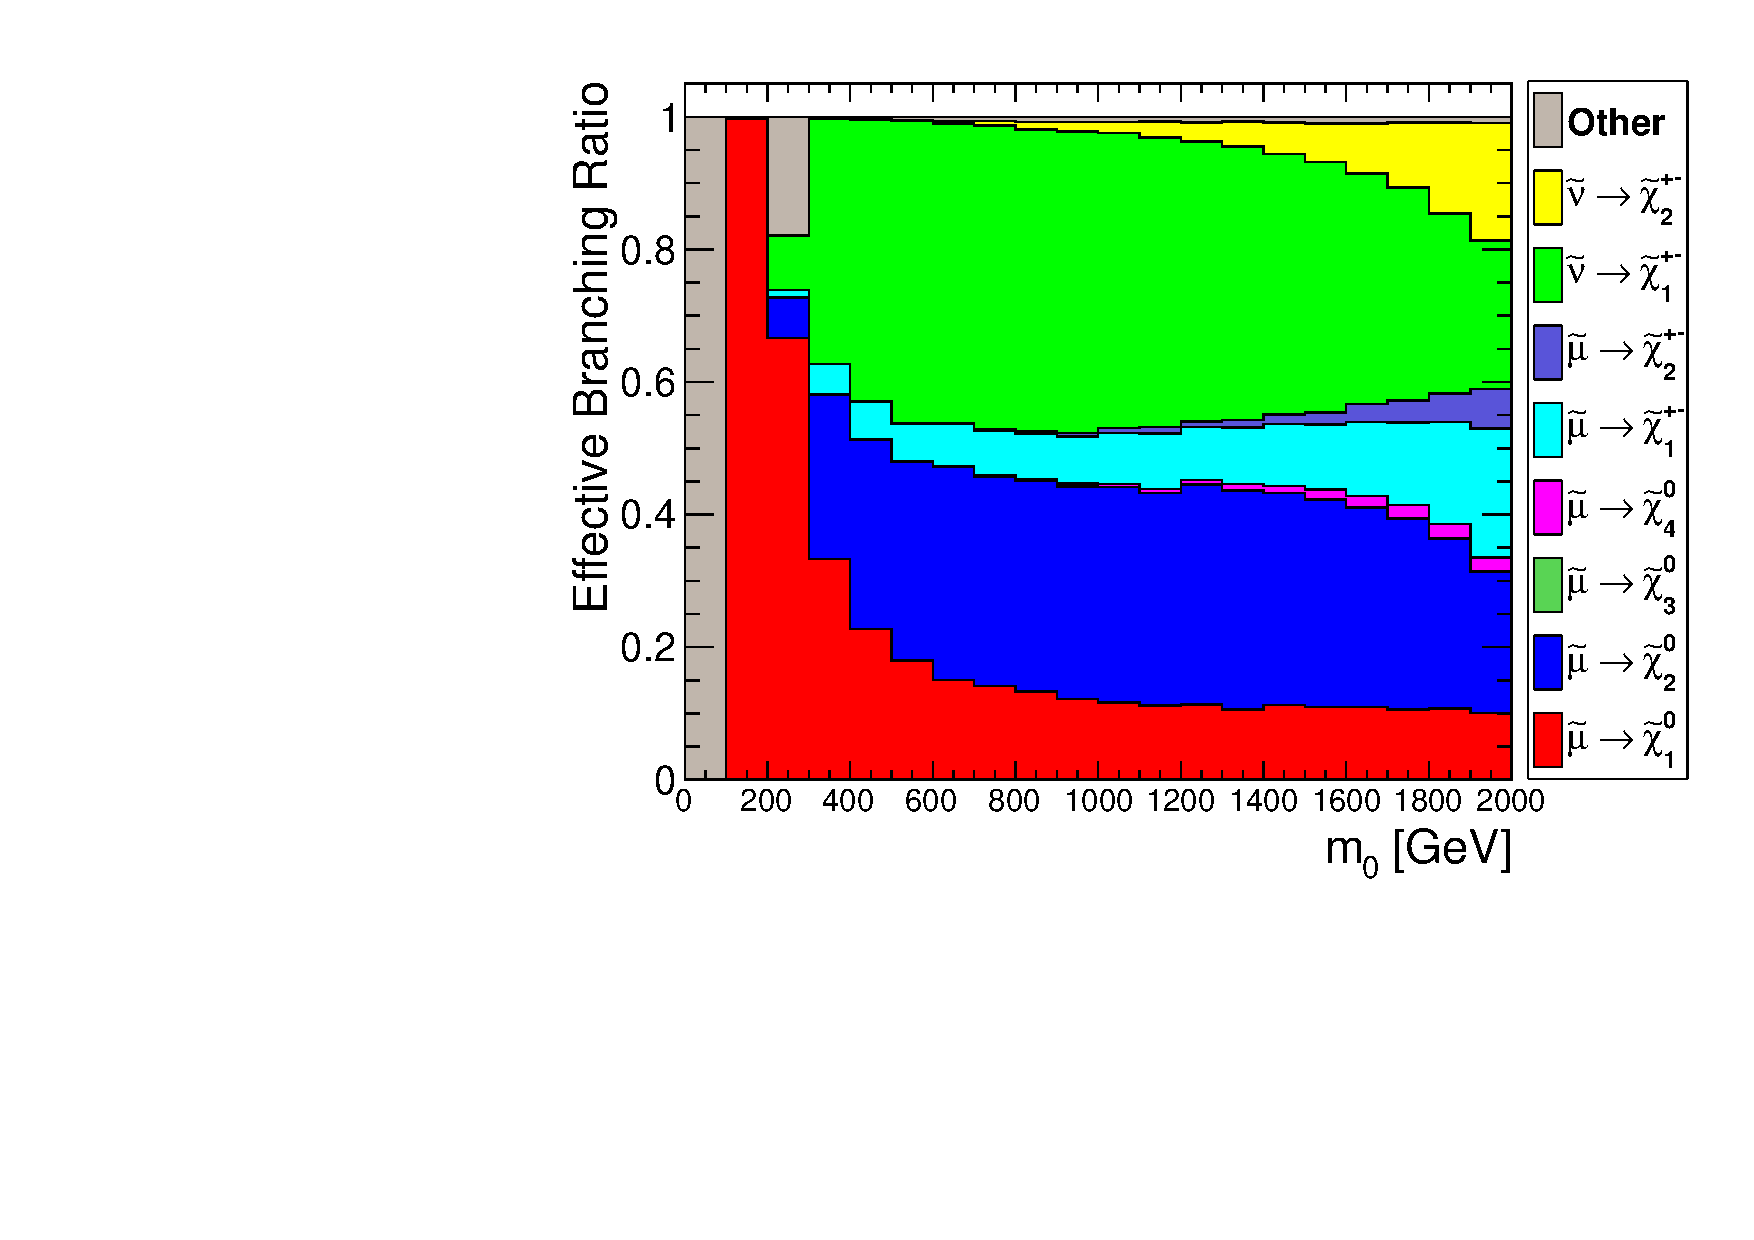
\includegraphics[width=\textwidth]{plots/hCrossRatio550.pdf}
    \caption{$m_{1/2} = 550\,\text{GeV}$\label{fig:crossratio550}}
  \end{subfigure}
  \begin{subfigure}[b]{0.495\textwidth}
    \centering
    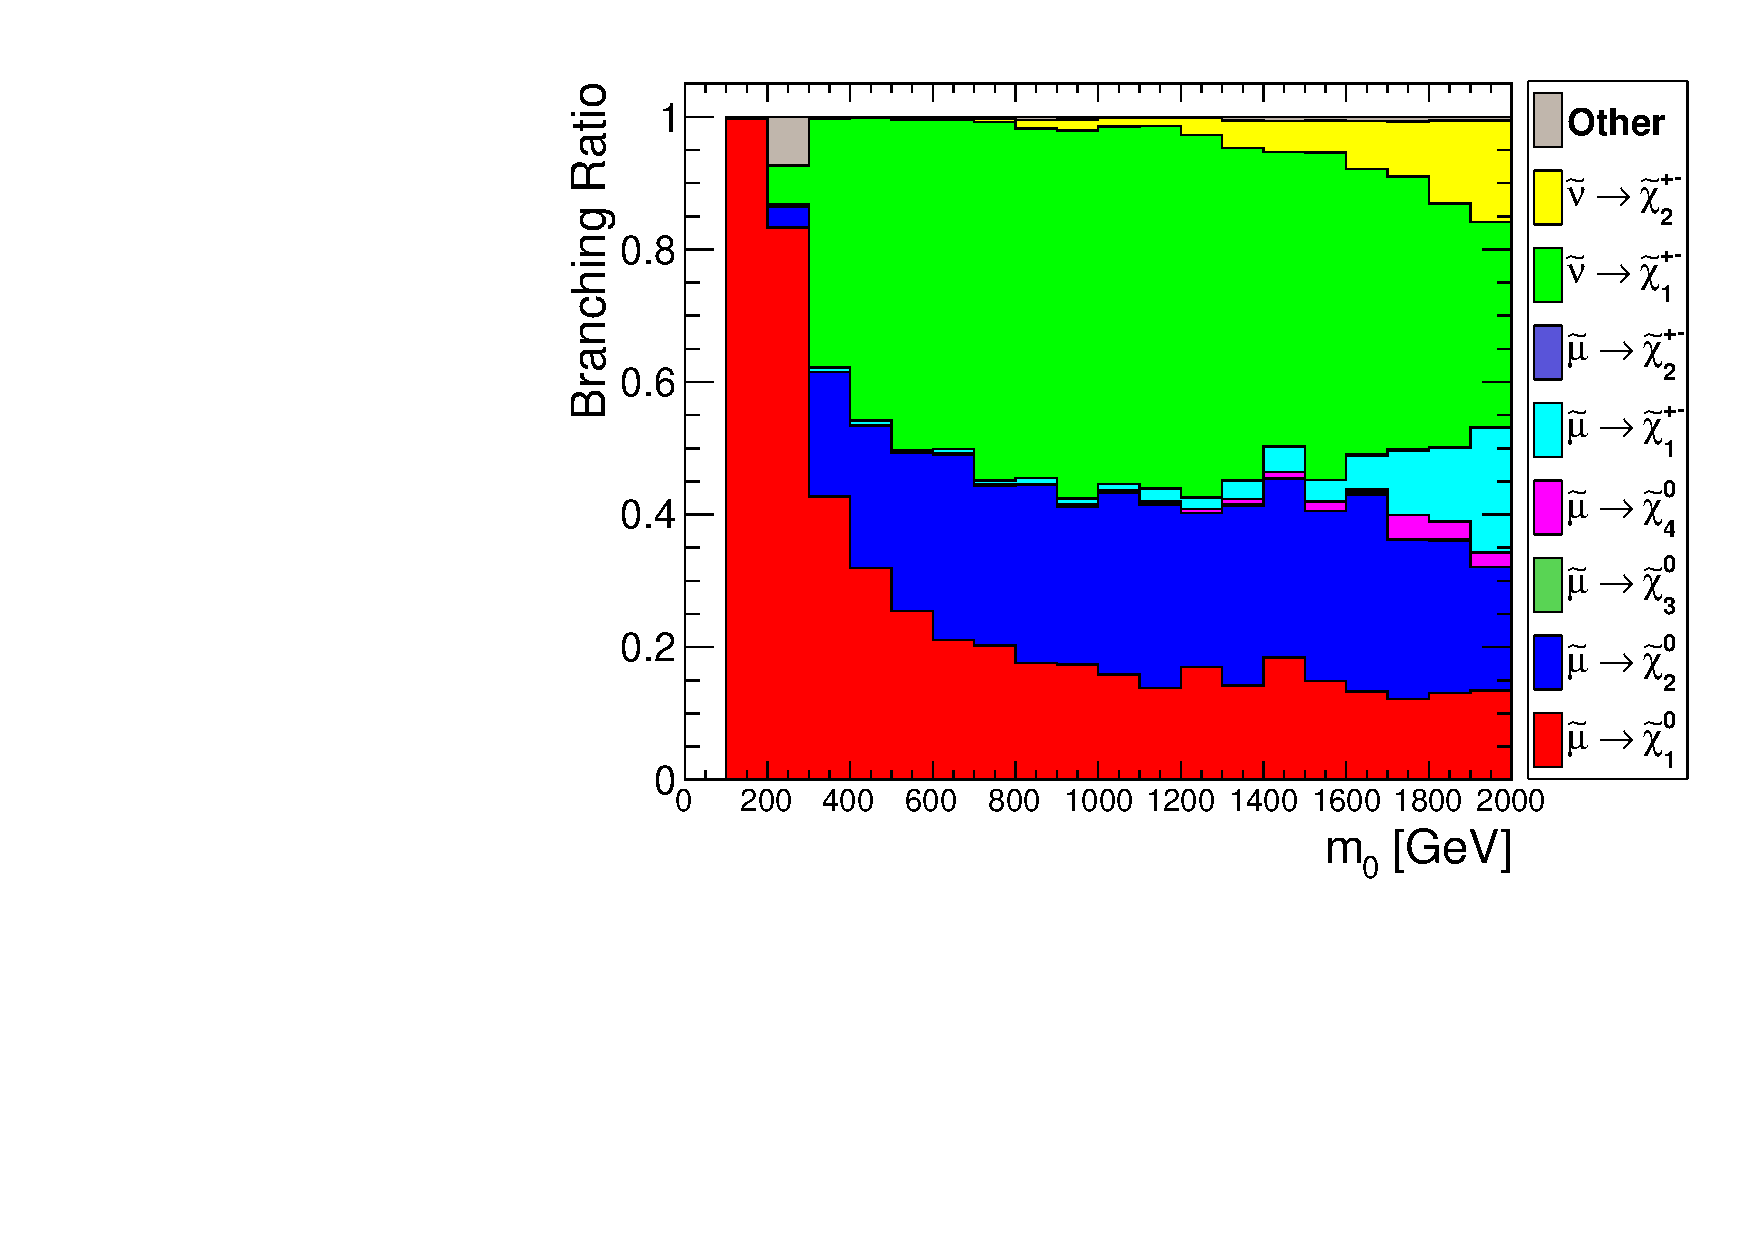
\includegraphics[width=\textwidth]{plots/hCutCrossRatio550.pdf}
    \caption{$m_{1/2} = 550\,\text{GeV}$\label{fig:cutcrossratio550}}
  \end{subfigure}

  \begin{subfigure}[b]{0.495\textwidth}
    \centering
    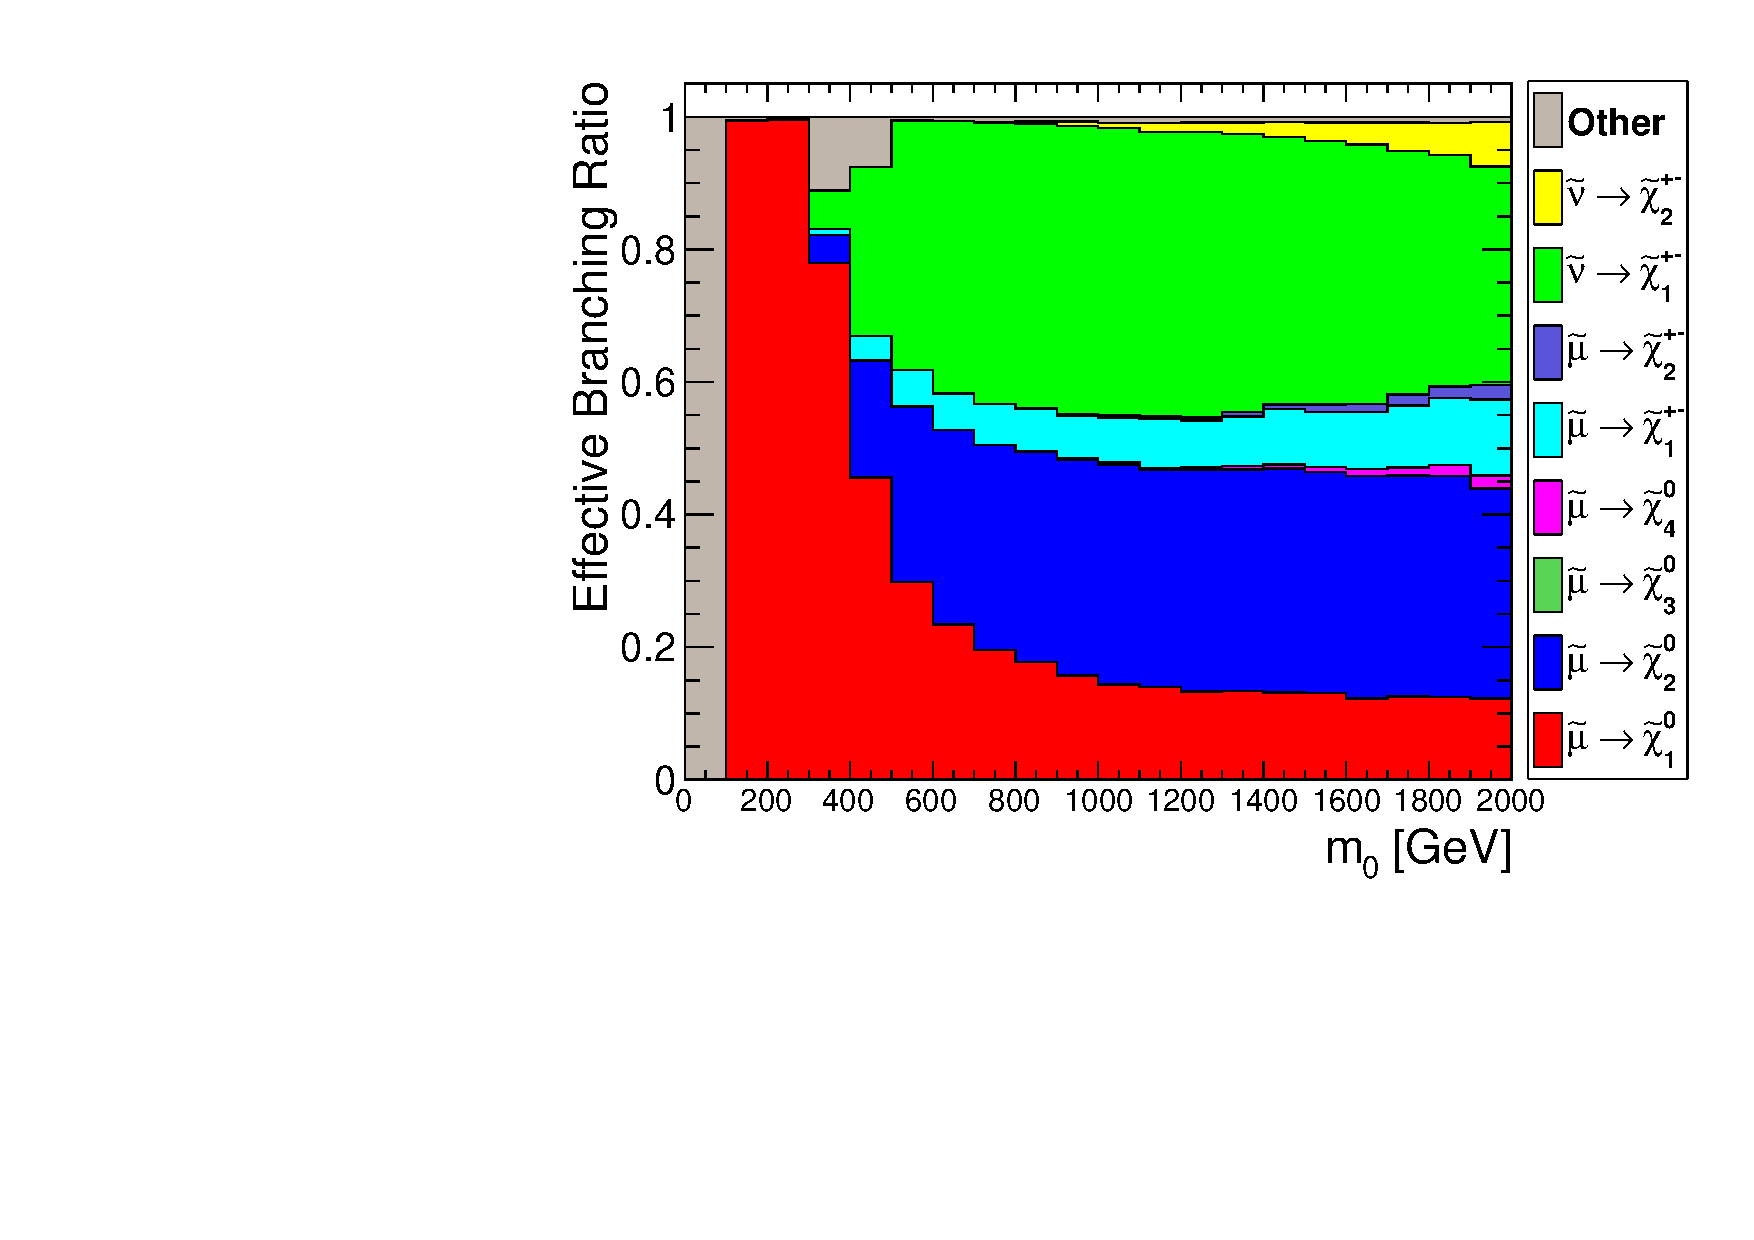
\includegraphics[width=\textwidth]{plots/hCrossRatio750.pdf}
    \caption{$m_{1/2} = 750\,\text{GeV}$\label{fig:crossratio750}}
  \end{subfigure}
  \begin{subfigure}[b]{0.495\textwidth}
    \centering
    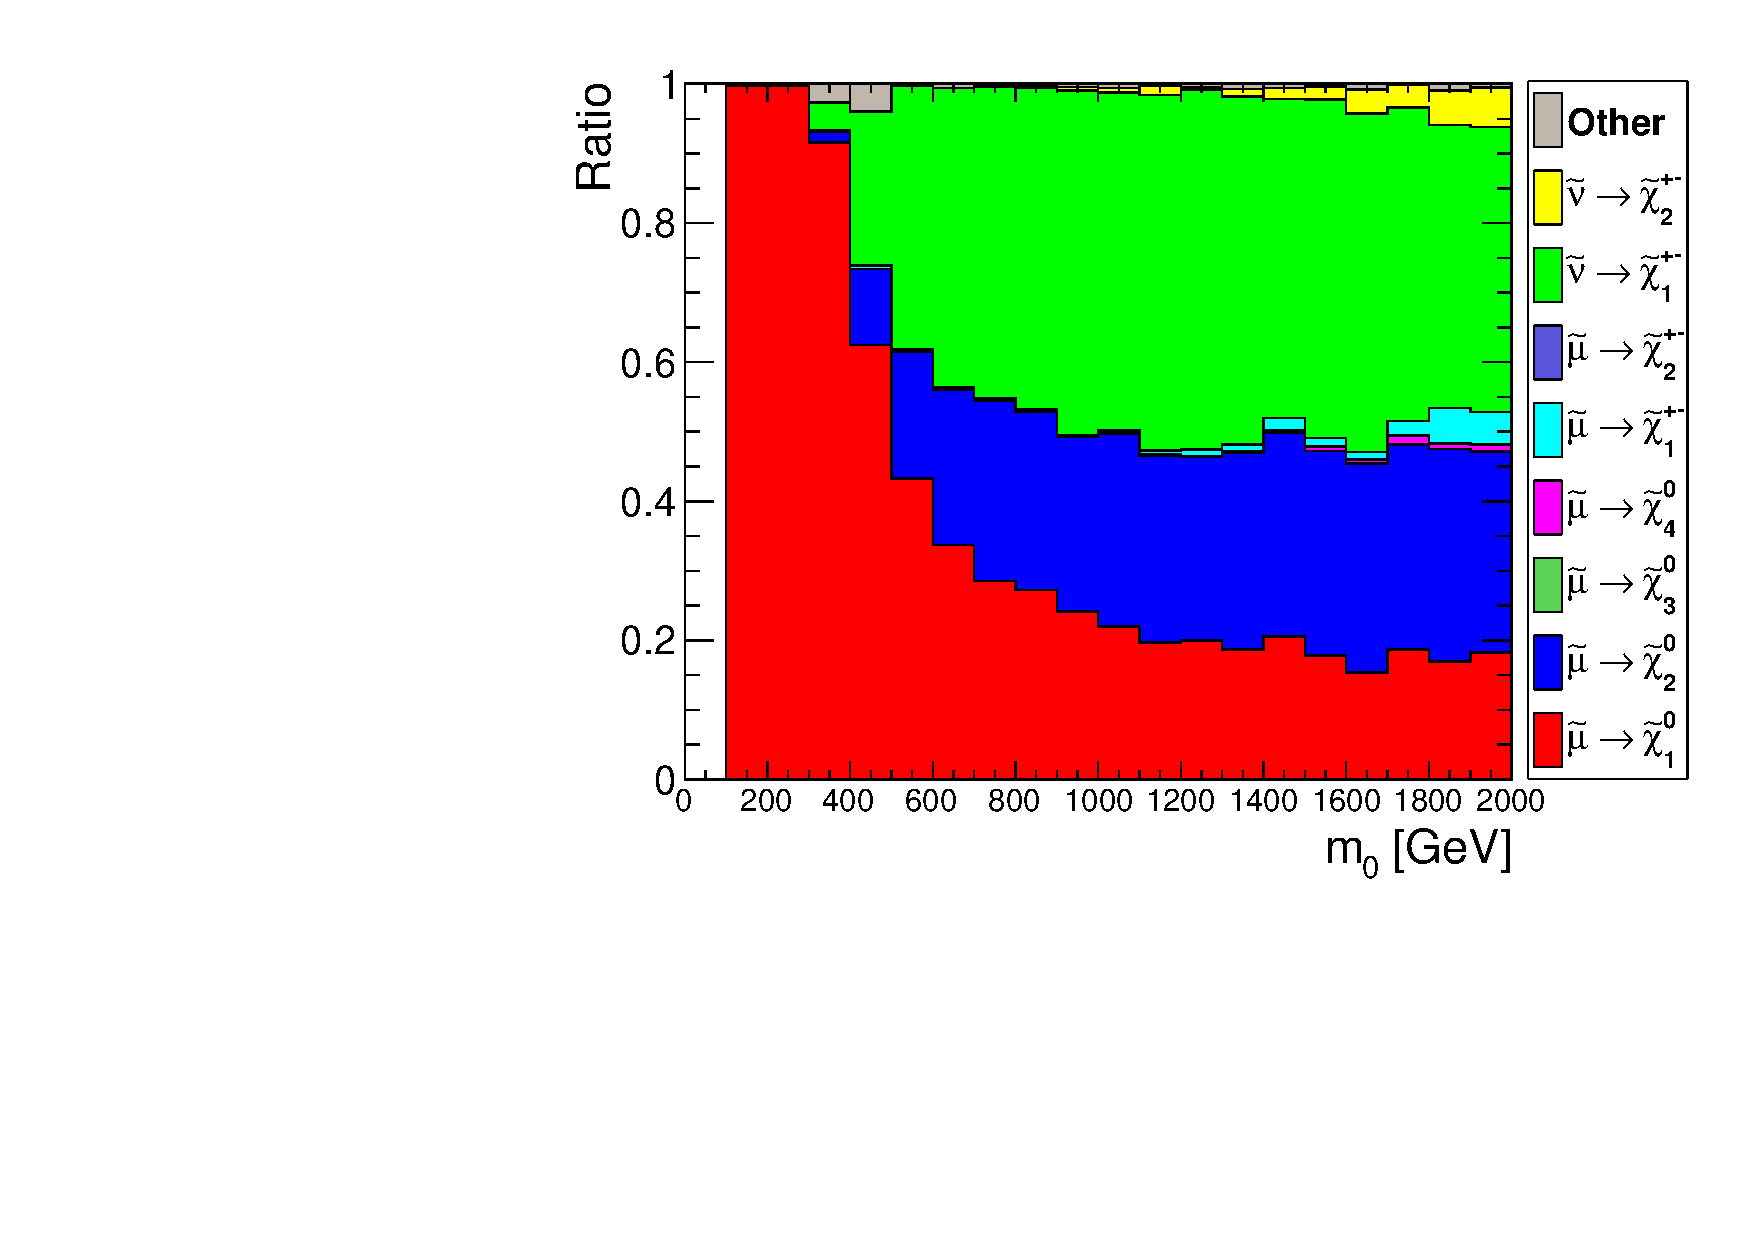
\includegraphics[width=\textwidth]{plots/hCutCrossRatio750.pdf}
    \caption{$m_{1/2} = 750\,\text{GeV}$\label{fig:cutcrossratio750}}
  \end{subfigure}

  \caption{Sum of all ERBs for the events from figure~\ref{fig:sigeff} for fixed values of $m_{1/2}$. All distributions on the left show the MU2J2 case, while the ANA case is given on the right side. Each color represents the ERB from a different process.}
  \label{fig:crossratios}
\end{figure}

Taking the empty bins into account (Cf.~\ref{fig:sigeff}), $550\,\text{GeV}$ as a value for $m_{1/2}$ provides a reasonable overview shown in figures~\ref{fig:crossratio550} and \ref{fig:cutcrossratio550}. To ensure a similar behaviour over the entire $m_{1/2}$ range, two variations with a $200\,\text{GeV}$ difference in the value of $m_{1/2}$ are used for confirmation (Fig.~\ref{fig:crossratio350},~\ref{fig:cutcrossratio350},~\ref{fig:crossratio750} and \ref{fig:cutcrossratio750}). With the grey colour marking the remaining contribution, only a negligible part of the total EBR is not covered by the listed processes. Initially, this statement would contradict the first bin of the MU2J2 case. However, since a \textit{ratio} is being shown, this can be explained by the very low number of selected events in this region (Cf.~\ref{fig:sigeff}). The ANA case supports this explanation, as none of the events pass its requirements.

As one would expect, for higher sfermion masses the contribution from processes with heavier sparticles increases. However the conclusion that can be drawn from these distributions, is that three processes dominate the signature of this analysis' signal. This is only enhanced by transitioning from the MU2J2, to the ANA case. The corresponding Feynman graphs for each of the three processes are given in figure~\ref{fig:domprocesses}.

\begin{figure}[htb!]
  \centering
  \begin{subfigure}[b]{0.495\textwidth}
    \centering
    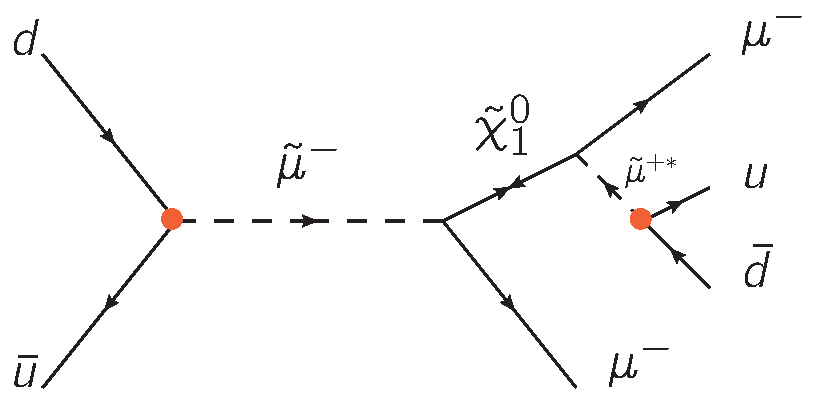
\includegraphics[width=\textwidth]{plots/rpv-resonant-smuon-samesign-mumuqq.pdf}
    \caption{\label{fig:resosmuneut1}}
  \end{subfigure}
  \begin{subfigure}[b]{0.495\textwidth}
    \centering
    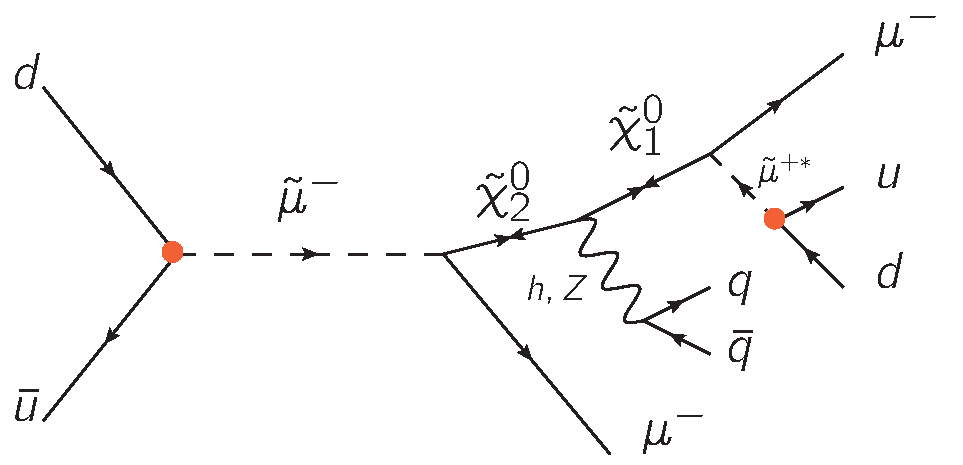
\includegraphics[width=\textwidth]{plots/rpv-resonant-smuon-neutralino2.pdf}
    \caption{\label{fig:resosmuneut2}}
  \end{subfigure}

  \begin{subfigure}[b]{0.495\textwidth}
    \centering
    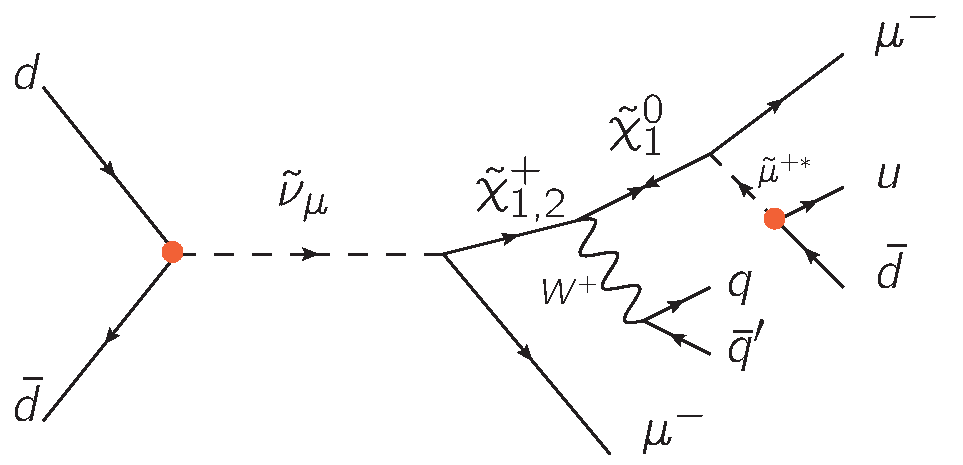
\includegraphics[width=\textwidth]{plots/rpv-resonant-sneutrino-chargino-mumuqq.pdf}
    \caption{\label{fig:resosneutcharg1}}
  \end{subfigure}

  \caption{Feynman graphs of the three dominant processes that lead to the signal signature. Each of the cascades leads to the neutralino LSP, which then decays through the $\lambda^\prime_{211}$ coupling, adding two jets and one muon to the final state.}
  \label{fig:domprocesses}
\end{figure}

\noindent As mentioned beforehand, after reaching the LSP through the cascade, the decay through the $\lambda^\prime_{211}$ leading to two jets and one muon is identical for every process. The simplest graph (Fig.~\ref{fig:resosmuneut1}) has its biggest contribution of up to almost $100\pct$ in the low $m_0$ region. It then quickly loses importance and remains at a constant level around $20\pct$. Both the other processes gain importance as the simple one loses it. Their contribution levels around $25\pct$ for the $\tilde{\mu} \rightarrow \tilde{\chi}^0_2$ and $45\pct$ for the $\tilde{\nu} \rightarrow \tilde{\chi}^\pm_1$ process for $500\,\text{GeV} < m_0 < 1600\,\text{GeV}$. Afterwards they decrease slowly.

This information can be used to allow for different interpretations of the results of this analysis. In addition to using the supersymmetric model, simplified models for the three Feynman graphs are an option. Since these types of models only focus on the physical parameters such as the particle mass and coupling strengths, it is easier to extrapolate from the results when working with different assumptions.



%%% Local Variables: 
%%% mode: latex
%%% TeX-master: "document"
%%% End: 

\chapter{Software \& Datasets}
\label{cha:datasets}

\section{Analysis Software}

With a signature of the signal determined, the necessary datasets for the analysis can be chosen. To access and work with these the \textsc{CMSSW} application framework~\cite{cmssw} is being used. Aside from providing the analysis tools, the collection of software also contributes to tasks like simulation, calibration, alignment and the event reconstruction. Due to a steady improvement in understanding the detector's and overall experiment's properties, an analysis is also dependent on the version of the \textsc{CMSSW} application framework. This analysis was performed using \verb+CMSSW_5_3_9_patch1+.

Both the simulated and recorded data are stored in the following three formats:

\begin{itemize}
\item \textsc{RAW} - This particular format stores the digital information provided by the detector and its system of triggers. At this stage, no physics objects have been reconstructed.
\item \textsc{RECO} - Derived from the \textsc{RAW}-format, the basic event reconstruction has been executed and its results are stored in this format.
\item \textsc{AOD} - Building upon the basic reconstruction, the contents of this format are high level physics objects. This provides most conventional physics analyses, including this one, with the necessary information to base their work upon.
\end{itemize}

By selecting the desired dataset content, the overall size of files can be reduced. For this purpose the \textsc{ACSUSYAnalysis} framework and its skimmer~\cite{acsusyana} are used. This allows for local storage in the form of a tree structure provided by \textsc{ROOT}~\cite{root}. For further analysis and visualization a combination of \textsc{ROOT} version $5.32.00$ and \textsc{findsusyb3}~\cite{findsusyb3} are employed. 


\section{Data}

As previously mentioned, the data that is going to be used for the search has been recorded by the CMS experiment (Sec.~\ref{sec:cms}). Only the four data taking periods from 2012 will be subject of this analysis. The center-of-mass energy for all of them is $\sqrt{s} = 8\,\text{TeV}$. Since two muons per event are a major part of the signature, the ``DoubleMu'' datasets are the most attractive ones, as they only contain events which activated at least one dimuon trigger. Table~\ref{tab:data} lists the chosen datasets.

\begin{table}[h!]
  \centering
  \begin{tabular}{|l|c|c|}
    \hline
    Datasets                                         & Run Range         & $\int \mathcal{L}$ [pb$^{-1}$] \\ \hline \hline
    \verb+/DoubleMu/Run2012A-22Jan2013-v1/AOD+       & $190645 - 193621$ & 876                            \\ \hline
    \verb+/DoubleMuParked/Run2012B-22Jan2013-v1/AOD+ & $193834 - 196531$ & 4409                           \\ \hline
    \verb+/DoubleMuParked/Run2012C-22Jan2013-v1/AOD+ & $198049 - 203002$ & 7017                           \\ \hline
    \verb+/DoubleMuParked/Run2012D-22Jan2013-v1/AOD+ & $203777 - 208686$ & 7369                           \\ \hline
    $\Sigma$                                         & $190645 - 208686$ & 19671                          \\ \hline
  \end{tabular}
  \caption{Overview of the data recorded by the CMS experiment, which is going to be used in this analysis. During the 2012 data taking period, the center-of-mass energy was set to $\sqrt{s} = 8\,\text{TeV}$.}
  \label{tab:data}
\end{table}

Dissecting the full name of a dataset gives different information about its contents. The first part, here DoubleMuParked, hints at the selected particle content. In this case, the \textit{Parked} version superseded the usual DoubleMu datasets by adding an additional offline trigger with a lower transverse momentum threshold. The second part of the name being the data taking period and the third one the date at which it was published. Unless the latter contains ``PromptReco'', the data has since been reprocessed with improved knowledge of the detector, leading to more precise measurements. The datasets which are subject of this analysis are part of the Winter13 ``ReReco'', short for rereconstruction. The data format, here ``AOD'', is given at the end.

In the second column, the run ranges are listed. Each run is composed of several sections with roughly equal luminosity. In the third column, the integrated luminosity for the individual run ranges is given. It is estimated from the average number of pixel clusters occurring in the silicon pixel detector (Sec.~\ref{sec:innertracker}) during an inelastic collision $\left< n \right>$.

\begin{equation}
  \label{eq:lumi}
  \mathcal{L} = \frac{\nu \left< n \right>}{\sigma_{\text{vis}}}
\end{equation}

\noindent The frequency of bunch crossings is given by $\nu$ and $\sigma_{\text{vis}}$ denotes the visible cross section. 

In general, only events from the certified list of properly reconstructed events \\ \verb+Cert_190456-208686_8TeV_PromptReco_Collisions12_JSON.txt+\footnote{It is often called the ``golden JSON'' as it is saved in the java script object notation.} are used. The integrated luminosity of this list is $19712\,\text{pb}^{-1}$. Comparing it to the sum of all used DoubleMuParked datasets, only a minuscule amount of events ($\sim 0.2\pct$) is not included in this analysis.

\section{Simulation}

As a general concept to differentiate between potential new physics and the standard model processes, this analysis compares the recorded data to a simulation. The difference between simulated and measured distributions of observables, more accurately the expected number of events, the probability of a discovery can be given. Due to the nature of this method, having a precise prediction from the simulation is essential. There is a strong dependence on the knowledge of the relevant standard model processes.

To take the probabilities for the occurrence of the various processes into account, a Monte-Carlo method is used for the simulation. While this describes the collision physics, the detector simulation is performed with \textsc{GEANT4}~\cite{geant41,geant42}. The next step of the simulation are the triggers, after which the events can be reconstructed using the \textsc{CMSSW} application framework.

\begin{table}[htbp!]
  \centering
  \begin{tabular}{|l|r|r|}
    % BEGIN RECEIVE ORGTBL datasetsmc
\hline
Monte Carlo Samples & $\sigma [\text{pb}^{-1}]$ & Weights \\
\hline
\hline
$Z/\gamma^* \rightarrow ll$ $(10\,\text{GeV} < m_{ll} < 50\,\text{GeV})$ & 762.45 & $1.25 \cdot 2.1029$ \\
$Z/\gamma^* \rightarrow ll$ $(50\,\text{GeV} < m_{ll})$ & 3503.71 $\star$$\star$ & $0.96 \cdot 2.2627$ \\
\hline
QCD $\mu_{p_\text{T} > 5\,\text{GeV}}$-enr. ($15\,\text{GeV} < p_{\text{T}} < 20\,\text{GeV}$) & 2738580.0 & 31271.3770 \\
QCD $\mu_{p_\text{T} > 5\,\text{GeV}}$-enr. ($20\,\text{GeV} < p_{\text{T}} < 30\,\text{GeV}$) & 1865500.0 & 4323.8677 \\
QCD $\mu_{p_\text{T} > 5\,\text{GeV}}$-enr. ($30\,\text{GeV} < p_{\text{T}} < 50\,\text{GeV}$) & 806298.0 & 1659.0218 \\
QCD $\mu_{p_\text{T} > 5\,\text{GeV}}$-enr. ($50\,\text{GeV} < p_{\text{T}} < 80\,\text{GeV}$) & 176187.6 & 334.3666 \\
QCD $\mu_{p_\text{T} > 5\,\text{GeV}}$-enr. ($80\,\text{GeV} < p_{\text{T}} < 120\,\text{GeV}$) & 40448.0 & 86.1222 \\
QCD $\mu_{p_\text{T} > 5\,\text{GeV}}$-enr. ($120\,\text{GeV} < p_{\text{T}} < 170\,\text{GeV}$) & 7463.940 & 17.2694 \\
QCD $\mu_{p_\text{T} > 5\,\text{GeV}}$-enr. ($170\,\text{GeV} < p_{\text{T}} < 300\,\text{GeV}$) & 2299.752 & 5.8981 \\
QCD $\mu_{p_\text{T} > 5\,\text{GeV}}$-enr. ($300\,\text{GeV} < p_{\text{T}} < 470\,\text{GeV}$) & 151.8048 & 0.3813 \\
QCD $\mu_{p_\text{T} > 5\,\text{GeV}}$-enr. ($470\,\text{GeV} < p_{\text{T}} < 600\,\text{GeV}$) & 11.79648 & 0.0613 \\
QCD $\mu_{p_\text{T} > 5\,\text{GeV}}$-enr. ($600\,\text{GeV} < p_{\text{T}} < 800\,\text{GeV}$) & 2.6902 & 0.0128 \\
QCD $\mu_{p_\text{T} > 5\,\text{GeV}}$-enr. ($800\,\text{GeV} < p_{\text{T}} < 1000\,\text{GeV}$) & 0.36878 & 0.0018 \\
QCD $\mu_{p_\text{T} > 5\,\text{GeV}}$-enr. ($1000\,\text{GeV} < p_{\text{T}}$) & 0.0849078 & 0.0004 \\
\hline
$t^+$ ($s$-channel) & $3.79 \pm 0.7$ $\star$$\star$$\star$ \cite{topxsec} & 0.5326 \\
$t^-$ ($s$-channel) & $1.76 \pm 0.01$ $\star$$\star$$\star$ \cite{topxsec} & 0.1332 \\
$t^+$ ($t$-channel) & $56.4^{+ 2.1}_{- 0.3}$ $\star$$\star$$\star$ \cite{topxsec} & 0.5733 \\
$t^-$ ($t$-channel) & $30.7 \pm 0.7$ $\star$$\star$$\star$ \cite{topxsec} & 6.0465 \\
$t^+$ ($tW$-channel) & $11.1 \pm 0.3$ $\star$$\star$$\star$ \cite{topxsec} & 0.5549 \\
$t^-$ ($tW$-channel) & $11.1 \pm 0.3$ $\star$$\star$$\star$ \cite{topxsec} & 0.4388 \\
\hline
$t\bar{t}$ & $234^{+10}_{-9}$ $\star$$\star$$\star$ & 0.2124 \\
\hline
$t\bar{t} + \gamma$ & 1.444 & 0.3967 \\
$t\bar{t} + W$ & $0.232 \pm 0.067$ $\star$ & 0.0210 \\
$t\bar{t} + WW$ & 0.002037 & 0.0002 \\
$t\bar{t} + Z$ & $0.2057^{+0.019}_{-0.024}$ & 0.0193 \\
\hline
$W + \text{jets} \rightarrow l + \nu$ & 37509.0$\star$$\star$ & 12.7853 \\
\hline
$W + \gamma \rightarrow l + \nu + 2 \mu$ & 1.914 & 0.1255 \\
$WW + \text{jets} \rightarrow 2 l + 2 \nu$ & $5.885 \pm 0.396$ $\star$ & 0.0599 \\
$WZ + \text{jets} \rightarrow 2 l + 2 q$ & $2.293 \pm 0.126$ $\star$ & 0.0140 \\
$WZ + \text{jets} \rightarrow 2 q + l \nu$ & $7.495 \pm 0.455$ $\star$ & 0.0507 \\
$WZ + \text{jets} \rightarrow 3 l + \nu$ & $1.105 \pm 0.066$ $\star$ & 0.0108 \\
$ZZ + \text{jets} \rightarrow 2 l + 2 \nu$ & $0.358 \pm 0.019$ $\star$ & 0.0074 \\
$ZZ + \text{jets} \rightarrow 2 l + 2 q$ & $1.251 \pm 0.065$ $\star$ & 0.0127 \\
$ZZ + \text{jets} \rightarrow 4 l$ & $0.181 \pm 0.009$ $\star$ & 0.0007 \\
\hline
$WWW$ & $0.08058^{+4.7\,\pct}_{-3.9\,\pct}$ $\star$ & 0.0072 \\
$WWZ$ & $0.05795^{+5.6\,\pct}_{-4.6\,\pct}$ $\star$ & 0.0051 \\
$WZZ$ & $0.01968^{+6.0\,\pct}_{-4.9\,\pct}$ $\star$ & 0.0018 \\
$ZZZ$ & $0.005527^{+2.7\,\pct}_{-2.4\,\pct}$ $\star$ & 0.0005 \\
\hline
$W^-W^-$ & 0.08888 & 0.0181 \\
$W^+W^+$ & 0.2482 & 0.0488 \\
$WW$-DoubleParton & 0.5879 & 0.0139 \\
\hline
    % END RECEIVE ORGTBL datasetsmc
  \end{tabular}
  \caption{List of all Monte Carlo samples that are considered as backgrounds for this analysis. Leading order cross sections are unmarked, while the stars indicate NLO ($\star$), NNLO($\star$$\star$) and approx. NNLO($\star$$\star$$\star$) calculations. Unless noted otherwise, the LO cross sections are taken from the generator output and the higher order ones are from~\cite{xsec}.}
  \label{tab:mcsamples}
\end{table}

\begin{comment}
  #+ORGTBL: SEND datasetsmc orgtbl-to-latex :splice t :no-escape t
  |---------------------------------------------------------------------------------------------------+-------------------------------------------------------------+---------------------|
  | Monte Carlo Samples                                                                               | $\sigma [\text{pb}^{-1}]$                                   |             Weights |
  |---------------------------------------------------------------------------------------------------+-------------------------------------------------------------+---------------------|
  |---------------------------------------------------------------------------------------------------+-------------------------------------------------------------+---------------------|
  | $Z/\gamma^* \rightarrow ll$ $(10\,\text{GeV} < m_{ll} < 50\,\text{GeV})$                          | 762.45                                                      | $1.25 \cdot 2.1029$ |
  | $Z/\gamma^* \rightarrow ll$ $(50\,\text{GeV} < m_{ll})$                                           | 3503.71 $\star$$\star$                                      | $0.96 \cdot 2.2627$ |
  |---------------------------------------------------------------------------------------------------+-------------------------------------------------------------+---------------------|
  | QCD $\mu_{p_\text{T} > 5\,\text{GeV}}$-enr. ($15\,\text{GeV} < p_{\text{T}} < 20\,\text{GeV}$)    | 2738580.0                                                   |          31271.3770 |
  | QCD $\mu_{p_\text{T} > 5\,\text{GeV}}$-enr. ($20\,\text{GeV} < p_{\text{T}} < 30\,\text{GeV}$)    | 1865500.0                                                   |           4323.8677 |
  | QCD $\mu_{p_\text{T} > 5\,\text{GeV}}$-enr. ($30\,\text{GeV} < p_{\text{T}} < 50\,\text{GeV}$)    | 806298.0                                                    |           1659.0218 |
  | QCD $\mu_{p_\text{T} > 5\,\text{GeV}}$-enr. ($50\,\text{GeV} < p_{\text{T}} < 80\,\text{GeV}$)    | 176187.6                                                    |            334.3666 |
  | QCD $\mu_{p_\text{T} > 5\,\text{GeV}}$-enr. ($80\,\text{GeV} < p_{\text{T}} < 120\,\text{GeV}$)   | 40448.0                                                     |             86.1222 |
  | QCD $\mu_{p_\text{T} > 5\,\text{GeV}}$-enr. ($120\,\text{GeV} < p_{\text{T}} < 170\,\text{GeV}$)  | 7463.940                                                    |             17.2694 |
  | QCD $\mu_{p_\text{T} > 5\,\text{GeV}}$-enr. ($170\,\text{GeV} < p_{\text{T}} < 300\,\text{GeV}$)  | 2299.752                                                    |              5.8981 |
  | QCD $\mu_{p_\text{T} > 5\,\text{GeV}}$-enr. ($300\,\text{GeV} < p_{\text{T}} < 470\,\text{GeV}$)  | 151.8048                                                    |              0.3813 |
  | QCD $\mu_{p_\text{T} > 5\,\text{GeV}}$-enr. ($470\,\text{GeV} < p_{\text{T}} < 600\,\text{GeV}$)  | 11.79648                                                    |              0.0613 |
  | QCD $\mu_{p_\text{T} > 5\,\text{GeV}}$-enr. ($600\,\text{GeV} < p_{\text{T}} < 800\,\text{GeV}$)  | 2.6902                                                      |              0.0128 |
  | QCD $\mu_{p_\text{T} > 5\,\text{GeV}}$-enr. ($800\,\text{GeV} < p_{\text{T}} < 1000\,\text{GeV}$) | 0.36878                                                     |              0.0018 |
  | QCD $\mu_{p_\text{T} > 5\,\text{GeV}}$-enr. ($1000\,\text{GeV} < p_{\text{T}}$)                   | 0.0849078                                                   |              0.0004 |
  |---------------------------------------------------------------------------------------------------+-------------------------------------------------------------+---------------------|
  | $t^+$ ($s$-channel)                                                                               | $3.79 \pm 0.7$ $\star$$\star$$\star$ \cite{topxsec}         |              0.5326 |
  | $t^-$ ($s$-channel)                                                                               | $1.76 \pm 0.01$ $\star$$\star$$\star$ \cite{topxsec}        |              0.1332 |
  | $t^+$ ($t$-channel)                                                                               | $56.4^{+ 2.1}_{- 0.3}$ $\star$$\star$$\star$ \cite{topxsec} |              0.5733 |
  | $t^-$ ($t$-channel)                                                                               | $30.7 \pm 0.7$ $\star$$\star$$\star$ \cite{topxsec}         |              6.0465 |
  | $t^+$ ($tW$-channel)                                                                              | $11.1 \pm 0.3$ $\star$$\star$$\star$ \cite{topxsec}         |              0.5549 |
  | $t^-$ ($tW$-channel)                                                                              | $11.1 \pm 0.3$ $\star$$\star$$\star$ \cite{topxsec}         |              0.4388 |
  |---------------------------------------------------------------------------------------------------+-------------------------------------------------------------+---------------------|
  | $t\bar{t}$                                                                                        | $234^{+10}_{-9}$ $\star$$\star$$\star$                      |              0.2124 |
  |---------------------------------------------------------------------------------------------------+-------------------------------------------------------------+---------------------|
  | $t\bar{t} + \gamma$                                                                               | 1.444                                                       |              0.3967 |
  | $t\bar{t} + W$                                                                                    | $0.232 \pm 0.067$ $\star$                                   |              0.0210 |
  | $t\bar{t} + WW$                                                                                   | 0.002037                                                    |              0.0002 |
  | $t\bar{t} + Z$                                                                                    | $0.2057^{+0.019}_{-0.024}$                                  |              0.0193 |
  |---------------------------------------------------------------------------------------------------+-------------------------------------------------------------+---------------------|
  | $W + \text{jets} \rightarrow l + \nu$                                                             | 37509.0$\star$$\star$                                       |             12.7853 |
  |---------------------------------------------------------------------------------------------------+-------------------------------------------------------------+---------------------|
  | $W + \gamma \rightarrow l + \nu + 2 \mu$                                                          | 1.914                                                       |              0.1255 |
  | $WW + \text{jets} \rightarrow 2 l + 2 \nu$                                                        | $5.885 \pm 0.396$ $\star$                                   |              0.0599 |
  | $WZ + \text{jets} \rightarrow 2 l + 2 q$                                                          | $2.293 \pm 0.126$ $\star$                                   |              0.0140 |
  | $WZ + \text{jets} \rightarrow 2 q + l \nu$                                                        | $7.495 \pm 0.455$ $\star$                                   |              0.0507 |
  | $WZ + \text{jets} \rightarrow 3 l + \nu$                                                          | $1.105 \pm 0.066$ $\star$                                   |              0.0108 |
  | $ZZ + \text{jets} \rightarrow 2 l + 2 \nu$                                                        | $0.358 \pm 0.019$ $\star$                                   |              0.0074 |
  | $ZZ + \text{jets} \rightarrow 2 l + 2 q$                                                          | $1.251 \pm 0.065$ $\star$                                   |              0.0127 |
  | $ZZ + \text{jets} \rightarrow 4 l$                                                                | $0.181 \pm 0.009$ $\star$                                   |              0.0007 |
  |---------------------------------------------------------------------------------------------------+-------------------------------------------------------------+---------------------|
  | $WWW$                                                                                             | $0.08058^{+4.7\,\pct}_{-3.9\,\pct}$ $\star$                 |              0.0072 |
  | $WWZ$                                                                                             | $0.05795^{+5.6\,\pct}_{-4.6\,\pct}$ $\star$                 |              0.0051 |
  | $WZZ$                                                                                             | $0.01968^{+6.0\,\pct}_{-4.9\,\pct}$ $\star$                 |              0.0018 |
  | $ZZZ$                                                                                             | $0.005527^{+2.7\,\pct}_{-2.4\,\pct}$ $\star$                |              0.0005 |
  |---------------------------------------------------------------------------------------------------+-------------------------------------------------------------+---------------------|
  | $W^-W^-$                                                                                          | 0.08888                                                     |              0.0181 |
  | $W^+W^+$                                                                                          | 0.2482                                                      |              0.0488 |
  | $WW$-DoubleParton                                                                                 | 0.5879                                                      |              0.0139 |
  |---------------------------------------------------------------------------------------------------+-------------------------------------------------------------+---------------------|
\end{comment}

All Monte Carlo samples that can produce two muons, two jets and are considered as backgrounds for this analysis are given in table~\ref{tab:mcsamples}. The samples were generated during the Summer12 period using \textsc{Pythia6}~\cite{pythia6} for QCD, \textsc{Powheg}~\cite{powheg,powhegst,powhegtt} for single and pair production of top-quarks and \textsc{Madgraph}~\cite{madgraph5} for most others. Details and the sample's paths are given in appendix~\ref{cha:mcsamppath}. In columns two and three, the cross section and weight of the specific process are given. The latter is necessary to adjust the generated number of events for each sample to the expected amount for a given luminosity. Producing Monte Carlos samples individually for each analysis would not only be inefficient, but also very resource intensive. Instead most samples are produced centrally, which is also the reason why the generated and expected number of events cannot be matched. The formula for calculating the weight is

\begin{equation}
  \label{eq:weight}
  w = f \cdot \frac{\sigma \cdot \mathcal{L}_{\text{int}}}{N}.
\end{equation}

\noindent The variable parameters are the cross section $\sigma$ and the number of generated events $N$. The integrated luminosity $\mathcal{L}_{\text{int}}$ is set through the amount of recorded data. An additional scaling factor $f$ can be introduced to account for effects like higher order corrections to a crossection. It is set to $1$ for all values shown in the table, except for the Drell-Yan processes. Their weights are given as a product, where $f$ is given as the first factor. The way these scaling factors are determined is described in an upcoming section (Sec.~\ref{sec:scaling}).

In all following distributions, groups of backgrounds are summarized under a single title to avoid cluttering. Table~\ref{tab:mcpooltitles} lists the names which will be used.

\begin{table}[!htb]
  \centering
  \begin{tabular}{|l|l|}
    % BEGIN RECEIVE ORGTBL mcpooltitles
\hline
Title & Monte Carlo Samples \\
\hline
Drell-Yan & Both $Z/\gamma^* \rightarrow ll$ \\
QCD & All QCD bins \\
Single-top & $t^\pm$ $s$-, $t$- and $tW$-channels \\
$t \bar{t}$ & $t \bar{t}$ \\
$t \bar{t} + V$ & $t \bar{t} + \gamma$, $t \bar{t} + W$, $t \bar{t} + WW$ and $t \bar{t} + Z$ \\
$W \rightarrow l \nu$ & $W + \text{jets} \rightarrow l + \nu$ \\
DiBoson & $W\gamma$ and all $WW$, $WZ$, $ZZ$ decay modes \\
$VVV$ & $WWW$, $WWZ$, $WZZ$ and $ZZZ$ \\
Rare Samples & $W^-W^-$, $W^+W^+$ and $WW$-DoubleParton \\
\hline
    % END RECEIVE ORGTBL mcpooltitles    
  \end{tabular}
  \caption{Arrangement of Monte Carlo titles in the distributions. Under each name on the left, the corresponding samples on the right are summarized.}
  \label{tab:mcpooltitles}
\end{table}
\begin{comment}
  #+ORGTBL: SEND mcpooltitles orgtbl-to-latex :splice t :skip 0 :no-escape t
  |-----------------------+-----------------------------------------------------------------------------|
  | Title                 | Monte Carlo Samples                                                         |
  |-----------------------+-----------------------------------------------------------------------------|
  | Drell-Yan             | Both $Z/\gamma^* \rightarrow ll$                                            |
  | QCD                   | All QCD bins                                                                |
  | Single-top            | $t^\pm$ $s$-, $t$- and $tW$-channels                                        |
  | $t \bar{t}$           | $t \bar{t}$                                                                 |
  | $t \bar{t} + V$       | $t \bar{t} + \gamma$, $t \bar{t} + W$, $t \bar{t} + WW$ and $t \bar{t} + Z$ |
  | $W \rightarrow l \nu$ | $W + \text{jets} \rightarrow l + \nu$                                       |
  | DiBoson               | $W\gamma$ and all $WW$, $WZ$, $ZZ$ decay modes                              |
  | $VVV$                 | $WWW$, $WWZ$, $WZZ$ and $ZZZ$                                               |
  | Rare Samples          | $W^-W^-$, $W^+W^+$ and $WW$-DoubleParton                                    |
  |-----------------------+-----------------------------------------------------------------------------|
\end{comment}

\begin{figure}[htb!]
  \centering
  \begin{subfigure}[b]{0.495\textwidth}
    \centering
    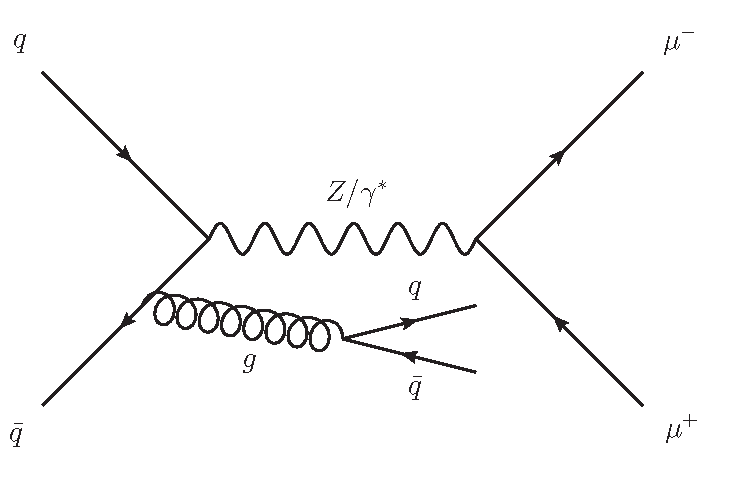
\includegraphics[width=\textwidth]{plots/dyll.pdf}
    \caption{\label{fig:dyll}}
  \end{subfigure}
  \begin{subfigure}[b]{0.495\textwidth}
    \centering
    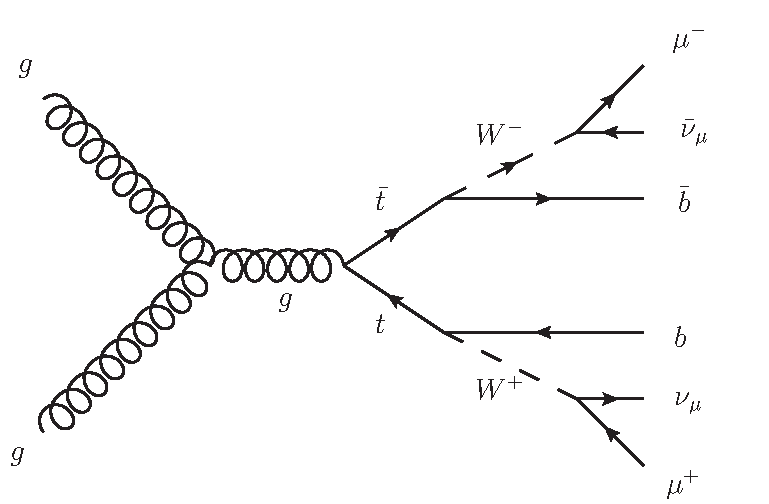
\includegraphics[width=\textwidth]{plots/ttbar.pdf}
    \caption{\label{fig:ttbar}}
  \end{subfigure}
  \caption{Drell-Yan~(\ref{fig:dyll}) and a $t\bar{t}$~(\ref{fig:ttbar}) feynman graph, which lead to a two muon and two jet signature. With their high crosssections, these two processes prove to be dominant Standard Model backgrounds for this analysis.}
  \label{fig:dyllttbar}
\end{figure}

The two Feynman graphs in figure~\ref{fig:dyllttbar} show the most dominant background processes before and after the same sign charge requirement, respectively. Drell-Yan processes with two muons (Fig.~\ref{fig:dyll}) are the prevalent background before applying the same sign charge requirement. An initial state which only requires one quark and its antimatter counterpart, leads to a high cross section. The two lepton final state can provide two muons, although the charge cannot have the same sign. An additional amount of two jets can be produced through radiation of additional bosons or unrelated interactions being misinterpreted. After applying the same sign charge requirement, top pair production (Fig.~\ref{fig:ttbar}) becomes the leading Standard Model process. Each top-quark is able to decay via the weak interaction, opening up the possibility of two leptons. However, their charge cannot be equal either. As a result, the events passing the same sign charge requirement have to have one faked muon. The likelihood for a muon to be a fake rises with the amount of hadronic activity. All Monte Carlo samples which are dominated by QCD multijet events and cannot lead to the necessary final state, will be used to estimate the amount of these contributions.


\subsection{Signal Simulation}
\label{sec:signal-sim}

While the previous section covers the simulation of the standard model background, it is also necessary to generate the supersymmetric model including the signal. Similarly to how said background is utilized, the simulation of the signal is used to estimate the likelihood of the measurement being described by supersymmetric processes.

To cover a variety of $R$-parity violating constrained MSSM scenarios, the $m_0$-$m_{1/2}$-phase space is subdivided into a grid. The SUSY mass spectra for each point in said grid are generated with \textsc{SoftSusy 3.3.5}~\cite{softsusy,sonnegueth} using the following parameters. The universal mass of scalar particles is increased from $100\,\text{GeV}$ to $2500\,\text{GeV}$ and the universal mass of fermonic ones from $100\,\text{GeV}$ to $1500\,\text{GeV}$. The size of each step is $100\,\text{GeV}$ for both variables. All remaining parameters are constant throughout the entire grid and are chosen to be

\begin{equation}
  \label{eq:gen-mssm-parameters}
  A_0 = 0, \quad \tan{\beta} = 20, \quad \text{sgn}\,\mu = +1, \quad \lambda^\prime_{211} = 0.01.
\end{equation}

As previously discussed (Cha.~\ref{cha:sig}), certain points in the parameter space do not favour the chosen signal signature while others do yield unphysical results. The former is strictly due the $\tilde{\tau}$-LSP configuration in the high $m_{1/2}$, low $m_0$ region, while the latter has three different reasons. Low values for $m_{1/2}$ and high ones $m_0$ can lead to no electroweak symmetry breaking, non-converging renormalization group equations or the production of tachyons. When generating the mass spectra, all of these scenarios are being excluded before the production. Overall, this leaves $287$ valid points in the phase space.

To actually produce the events, the leading order generator \textsc{CalcHep 3.4}~\cite{calchep} is being employed. Generated events are processed with the \textit{full} CMS detector simulation using the \verb+CMSSW_5_3_9_patch1+ framework. Running the full simulation on the entire grid of parameter points with sufficient statistics for each sample is resource intensive. Therefore a filter is applied at generator level (i.e. before parton showering and simulation) removing events that do not contain at least two muons. They also have to suffice the transverse momentum threshold of $10\,\text{GeV}$ for the leading muon and $5\,\text{GeV}$ for the sub leading one. These requirements are chosen such that they do not interfere with the trigger threshold of \verb+HLT_Mu17_TkMu8+.

In order to increase the accuracy of the \textsc{CalcHep} simulation, $k$-factors are determined as the ratio of a leading order to a next-to leading order cross section calculation~\cite{susyxstool}. They are then applied to the value provided by \textsc{CalcHep}. The branching fractions for the production of the smuon and sneutrino have to kept in mind. Both the evolution of the cross section as well as one the of $k$-factors are shown in figure~\ref{fig:susys-xs-kfactor}.

\begin{figure}[!htb]
  \centering
  \begin{subfigure}[b]{0.495\textwidth}
    \centering
    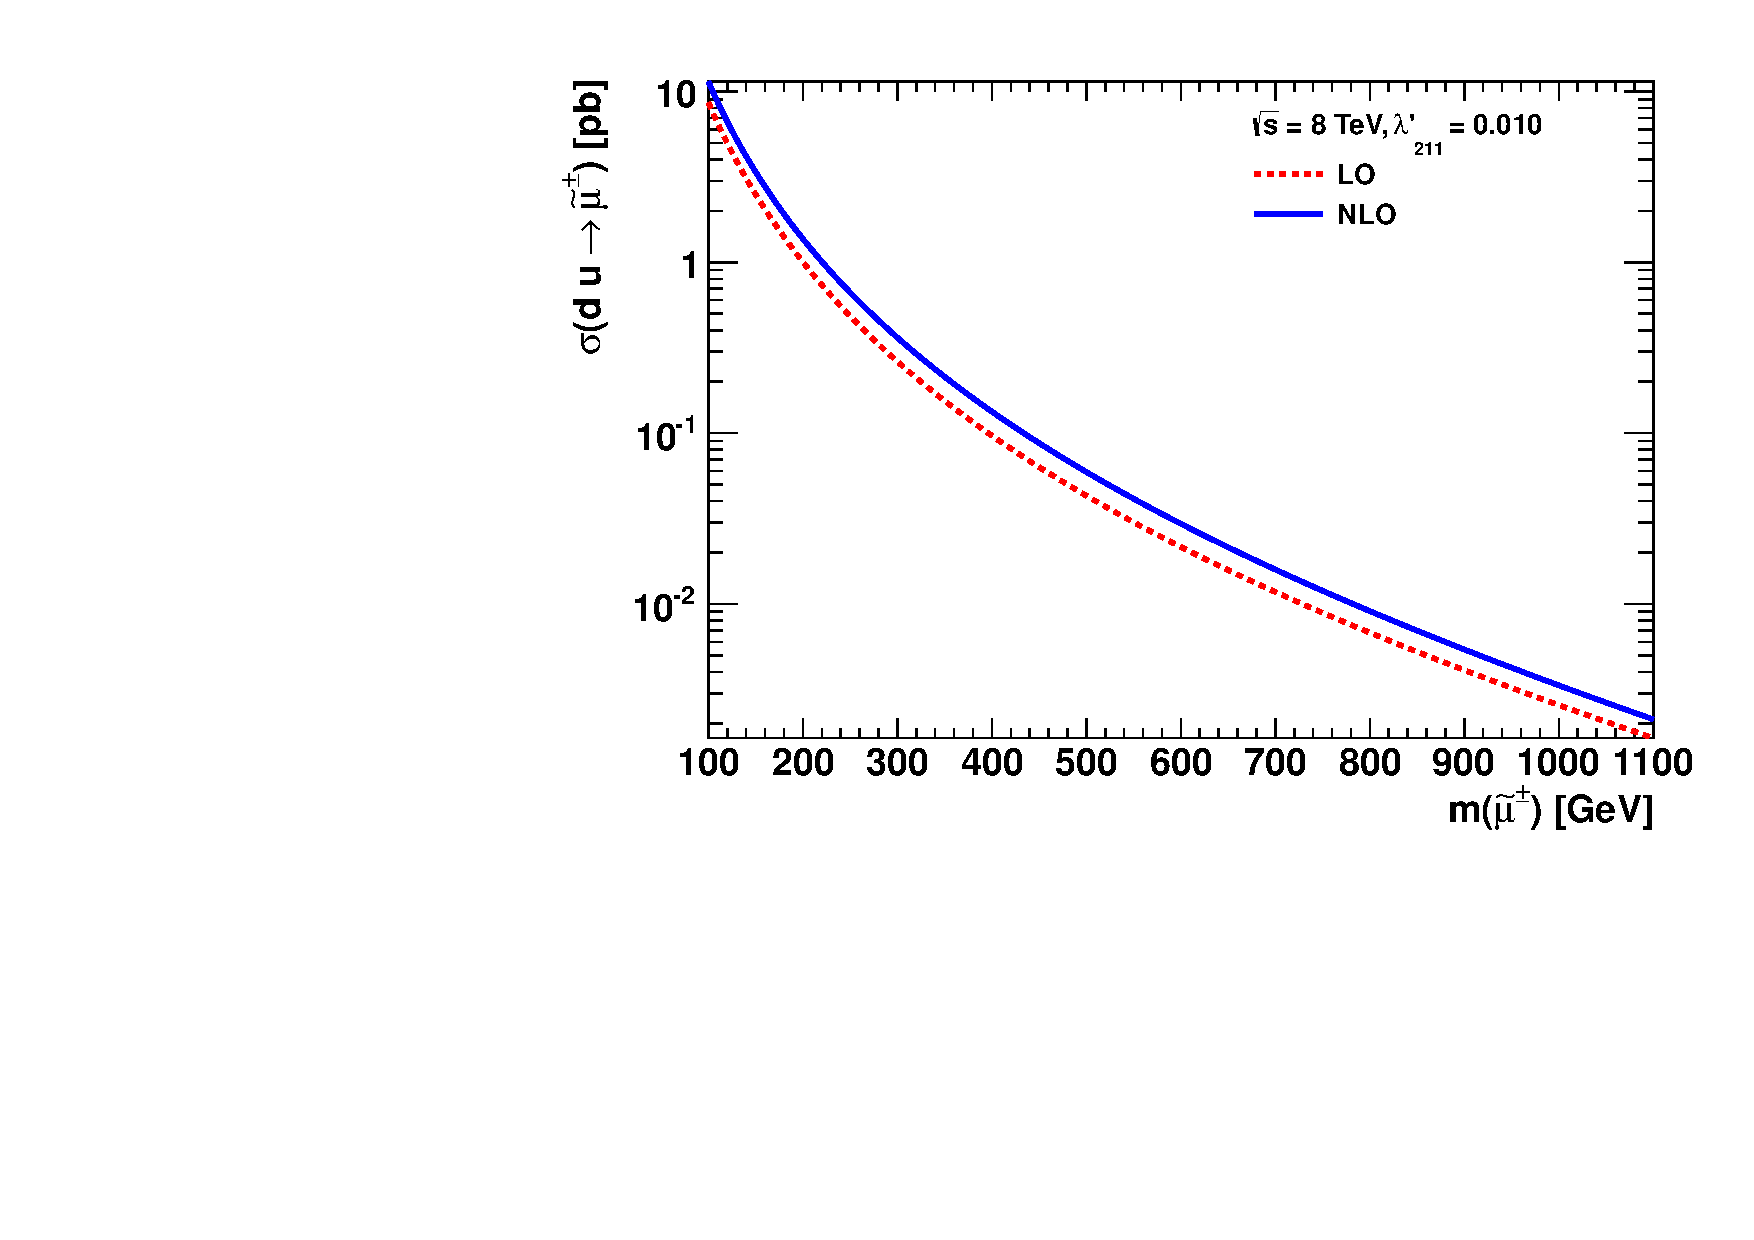
\includegraphics[width=\textwidth]{plots/xs.pdf}
    \caption{\label{fig:xs}}
  \end{subfigure}
  \begin{subfigure}[b]{0.495\textwidth}
    \centering
    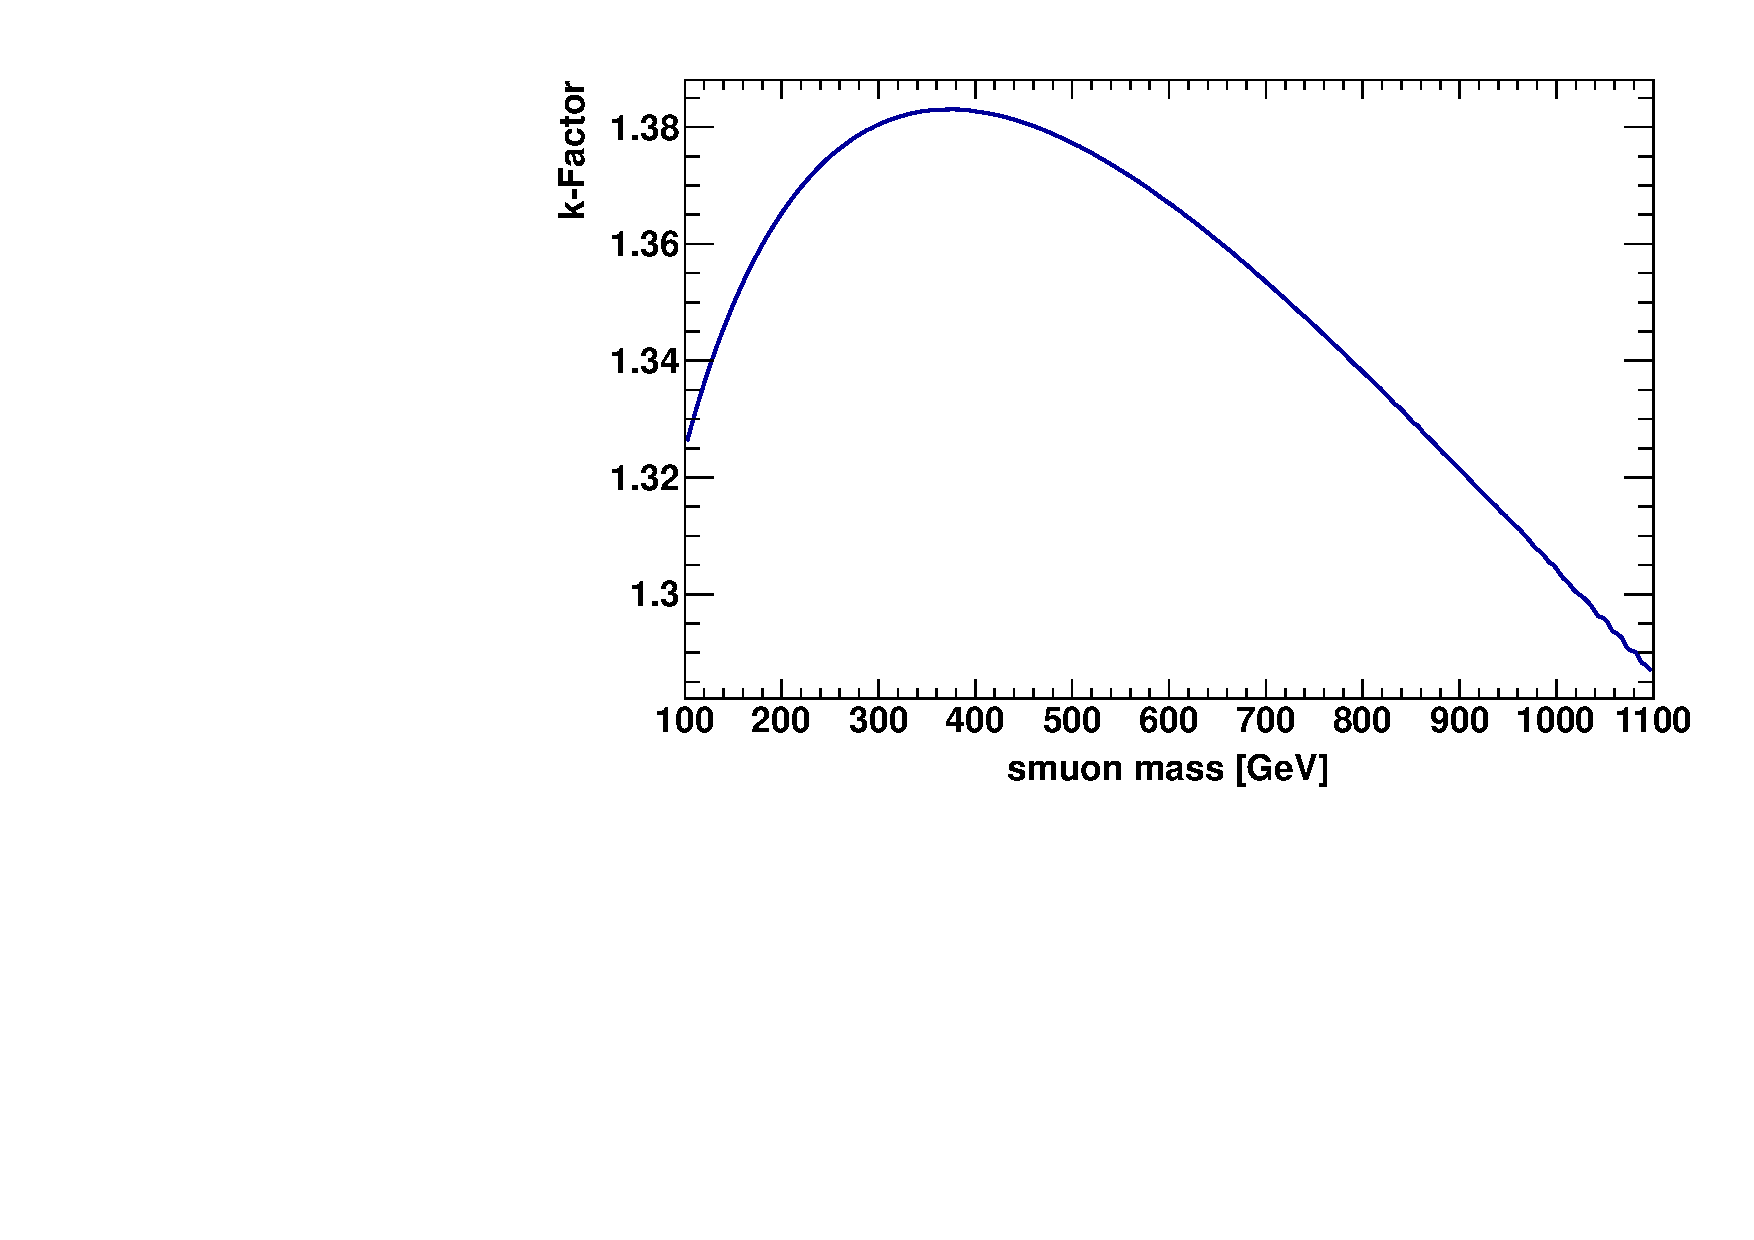
\includegraphics[width=\textwidth]{plots/k_smuon.pdf}
    \caption{\label{fig:k-smuon}}
  \end{subfigure}
  \caption{Cross section calculations for production of second generation sleptons via $\lambda^\prime_{211}$ (\ref{fig:xs}) and the subsequently determined $k$-factor for the smuon (\ref{fig:k-smuon}). The latter is the ratio of the LO and NLO cross section with respect to the smuons production branching ratio.}
  \label{fig:susys-xs-kfactor}
\end{figure}

\noindent Applying the $k$-factors to the \textsc{CalcHep} output, with respect to the branching ratios, yields the map of next-to leading orders cross sections used in the analysis. Said map is shown in figure~\ref{fig:susy-2dxs}.

\begin{figure}[!htb]
  \centering
  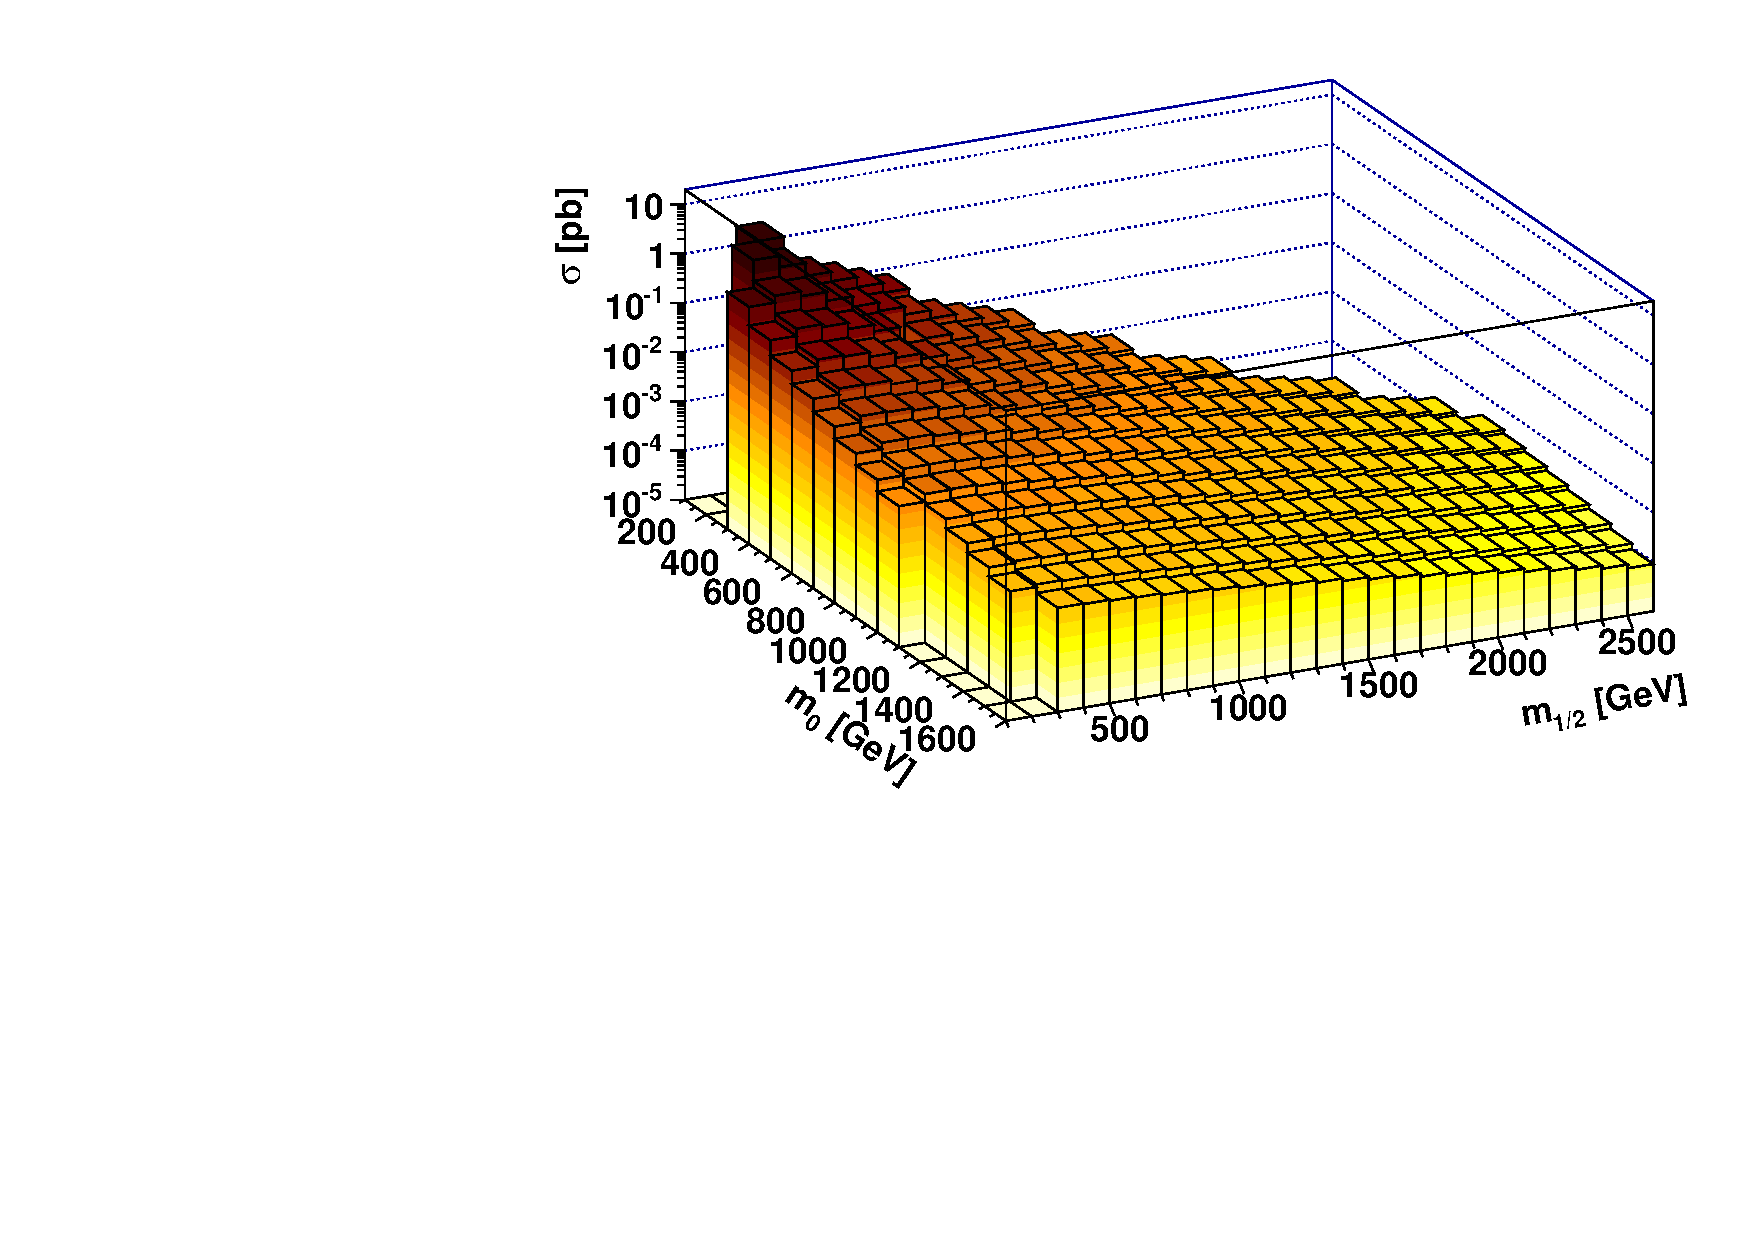
\includegraphics[width=0.6\textwidth]{plots/2dxs.pdf}
  \caption{NLO cross section map for the production of second generation sleptons used in the analysis.}
  \label{fig:susy-2dxs}
\end{figure}

For comparison, three points of the cMSSM parameter phase space will be shown in most of the upcoming distributions. The $m_0 = 300\,\text{GeV}$, $m_{1/2} = 300\,\text{GeV}$ and $m_0 = 1000\,\text{GeV}$, $m_{1/2} = 300\,\text{GeV}$, as well as the $m_0 = 1200\,\text{GeV}$, $m_0 = 1000\,\text{GeV}$ scenario. While the first two are within the range of existing limits (Sec.~\ref{sec:anamodel}), the latter is not. As such, only two of the corresponding cross sections are scaled to match said limits. Exemplary distributions displaying the different properties of the signal points are shown in figure~.


\section{Adjustments}

The Monte Carlo samples have been generated under assumptions that differ from the actual detector properties. Hence adjustments are necessary to ensure similar conditions before selecting events.


\subsection{Pileup Reweighting}
\label{sec:pileup}

During 2012 the average number of proton-proton collisions that occur for a single bunch-crossing is 21. The distribution for said data taking period is shown in figure~\ref{fig:pileup2012}. However, for the generated Monte Carlo samples the shape differs. Accommodating for that fact is an important step to allow for an accurate simulation of the experiment's conditions.

\begin{figure}[htb!]
  \centering
  \begin{subfigure}[b]{0.495\textwidth}
    \centering
    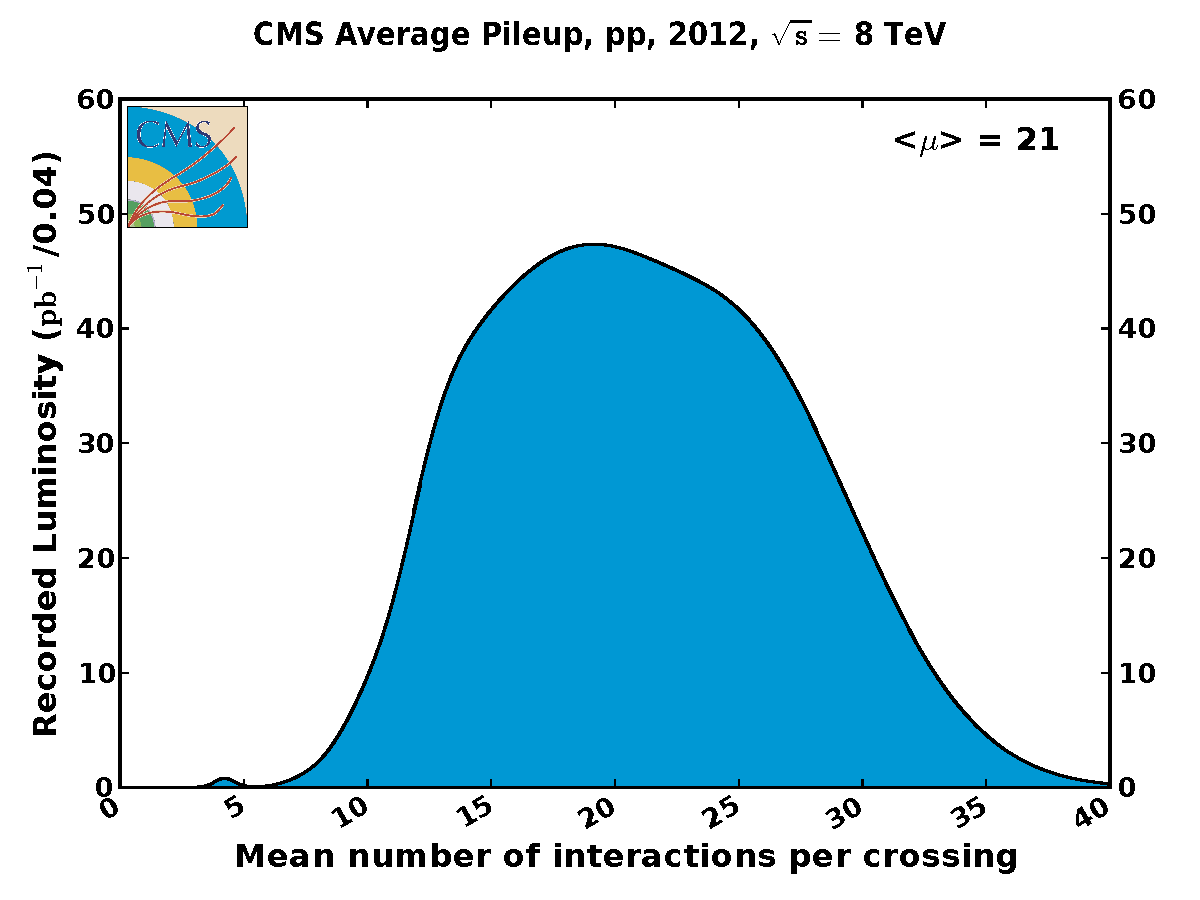
\includegraphics[width=\textwidth]{plots/pileup_pp_2012.pdf}
    \caption{\label{fig:pileup2012}}
  \end{subfigure}
  \begin{subfigure}[b]{0.495\textwidth}
    \centering
    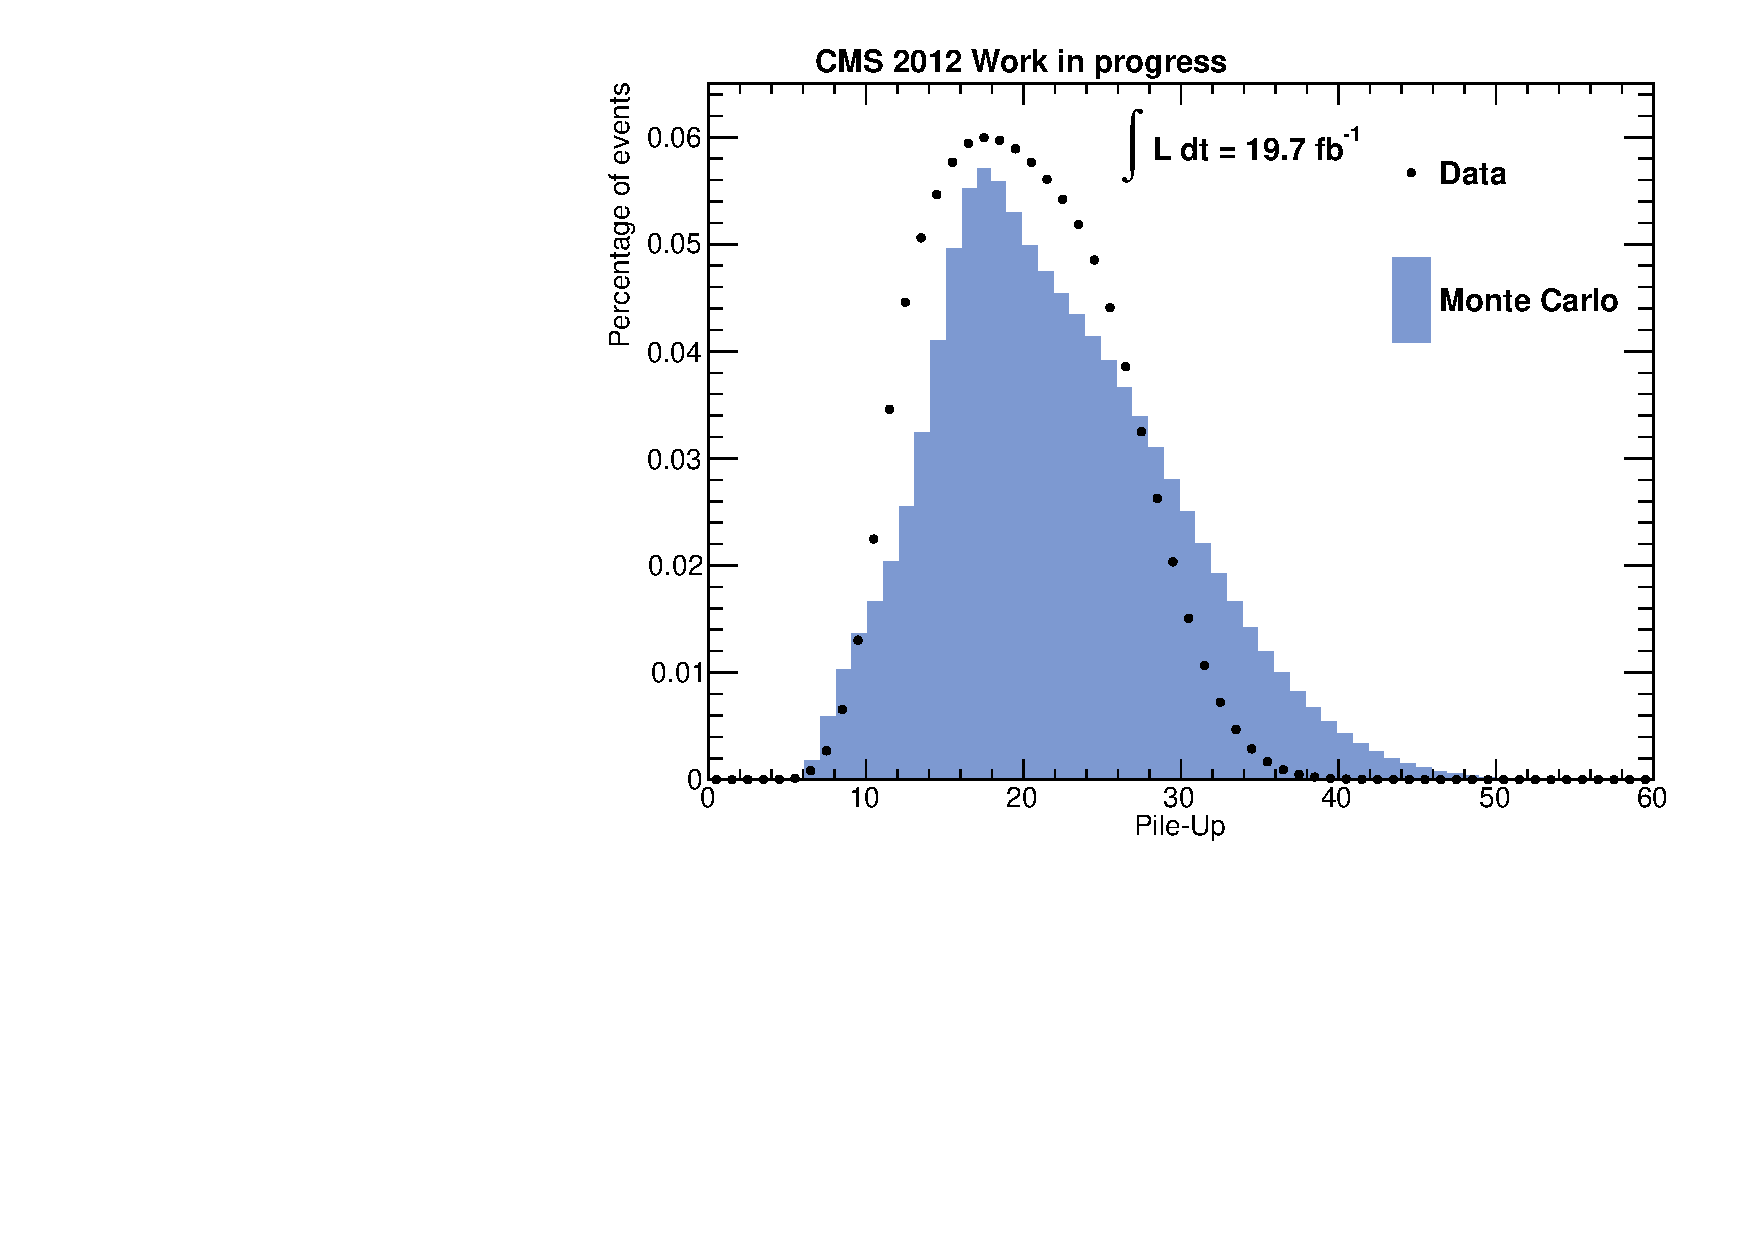
\includegraphics[width=\textwidth]{plots/pileup.pdf}
    \caption{\label{fig:pileup}}
  \end{subfigure}
  \caption{Average pileup for 2012 (\ref{fig:pileup2012}) and normalized pileup reweighting distribution (\ref{fig:pileup}).}
  \label{fig:pileups}
\end{figure}

To obtain the (true) number of interactions for each crossing, the instantaneous bunch-by-bunch luminosities are used as input. Combined with the total inelastic cross section, which amounts to $69400\,\mu\text{b}$ for 2012~\cite{pileup}, they can be used to calculate the aforementioned expected number of interactions for each luminosity section. While said cross section is entered manually into the script, the luminosities are extracted from a centrally maintained pileup file. In this analysis \verb+pileup_JSON_DCSONLY_190389-208686_All_2012_pixelcorr.txt+ has been used, which already includes corrections from the information provided by the pixel detector. Figure~\ref{fig:pileup2012} shows the histogram filled with the expected number of interactions for the 2012 data taking period. Complementary, figure~\ref{fig:pileup} shows the normalized distribution with the corresponding Monte Carlo entries. These bin contents for the simulated samples have also been gathered centrally and are taken from the dedicated TWiki website~\cite{pileupmc}. All samples in question have been produced with the Summer12 S10 scenario (c.f. app.~\ref{cha:mcsamppath}).

From the ratio of each bin a weight can be calculated and applied on an event by event basis for the analysis. Figure~\ref{fig:vtxn} provides a visualization of the effect of the reweighting.

\begin{figure}[htb!]
  \centering
  \begin{subfigure}[b]{0.495\textwidth}
    \centering
    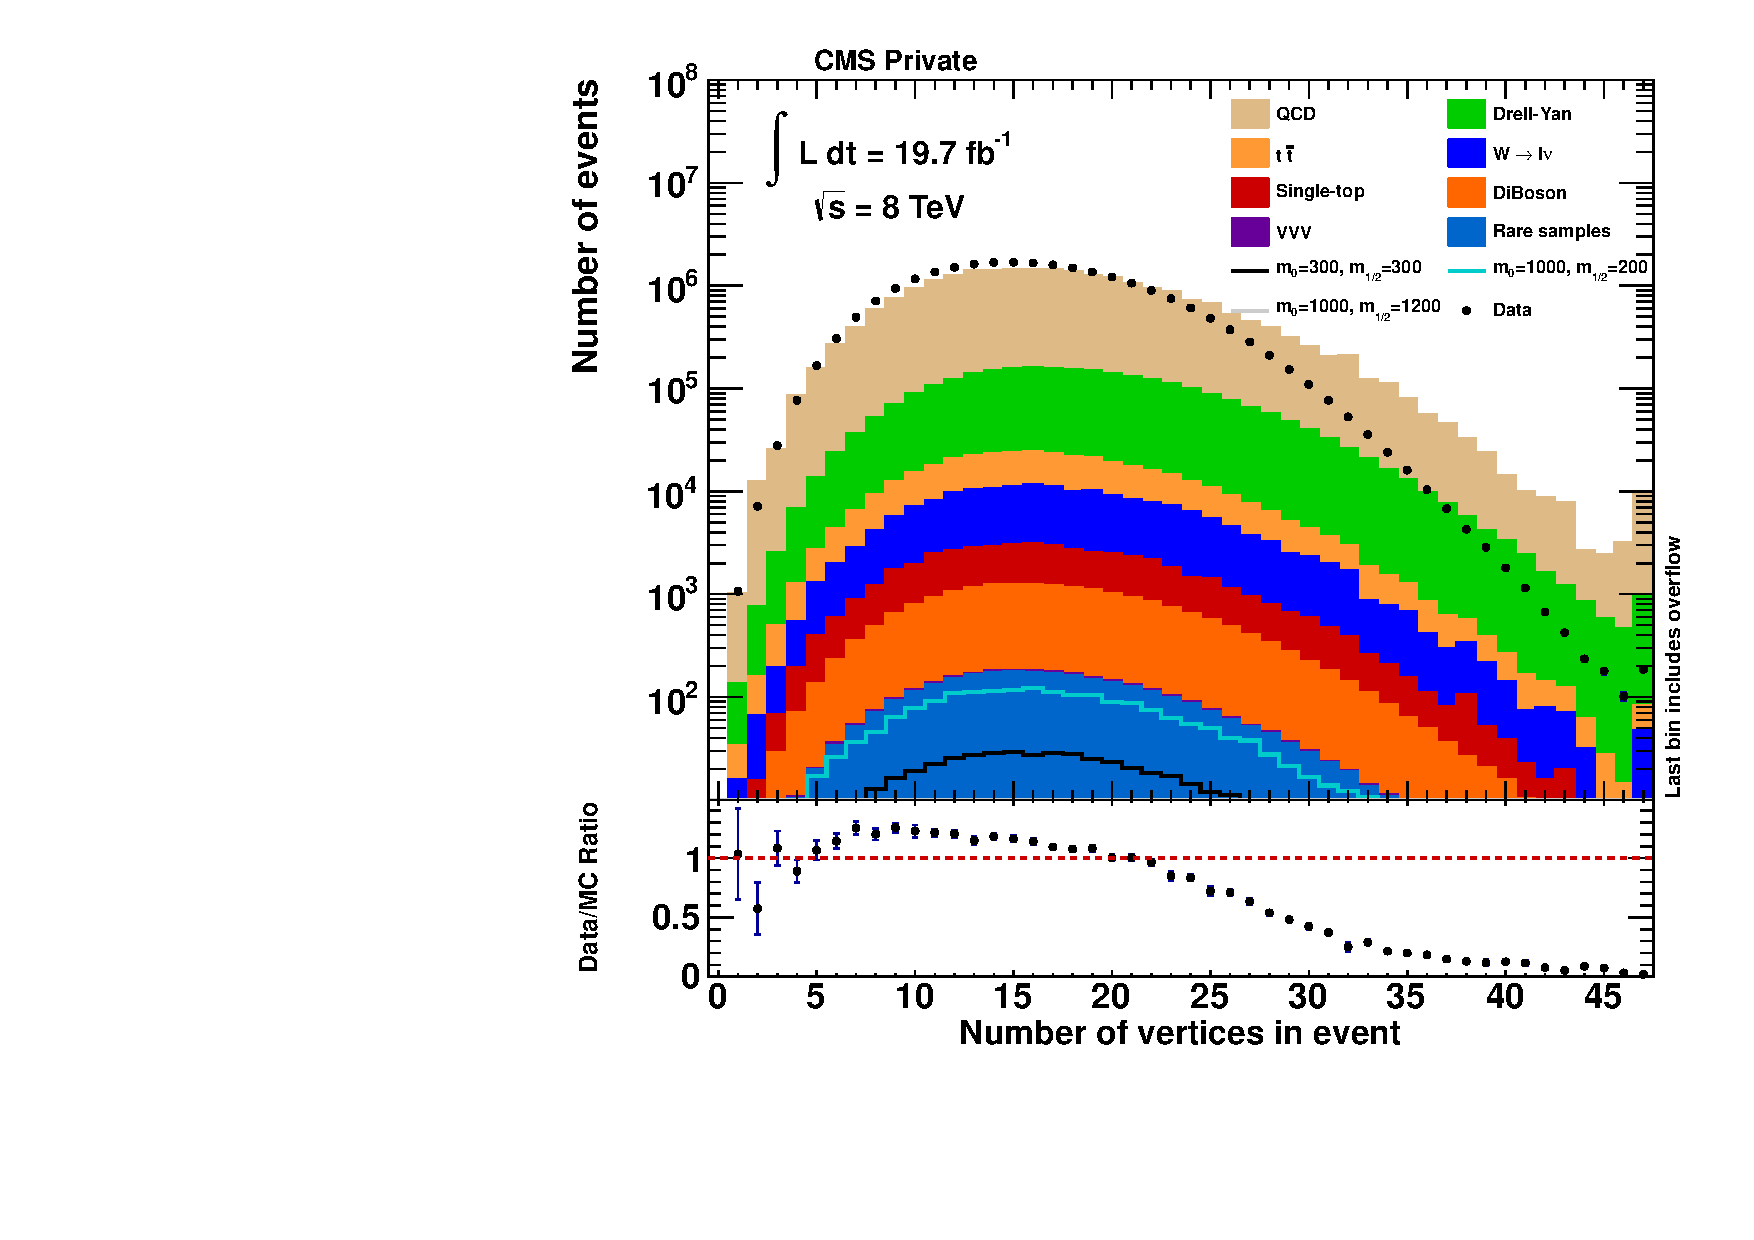
\includegraphics[width=\textwidth]{plots/vtx_n_nopu.pdf}
    \caption{\label{fig:vtx_n_nopu}}
  \end{subfigure}
  \begin{subfigure}[b]{0.495\textwidth}
    \centering
    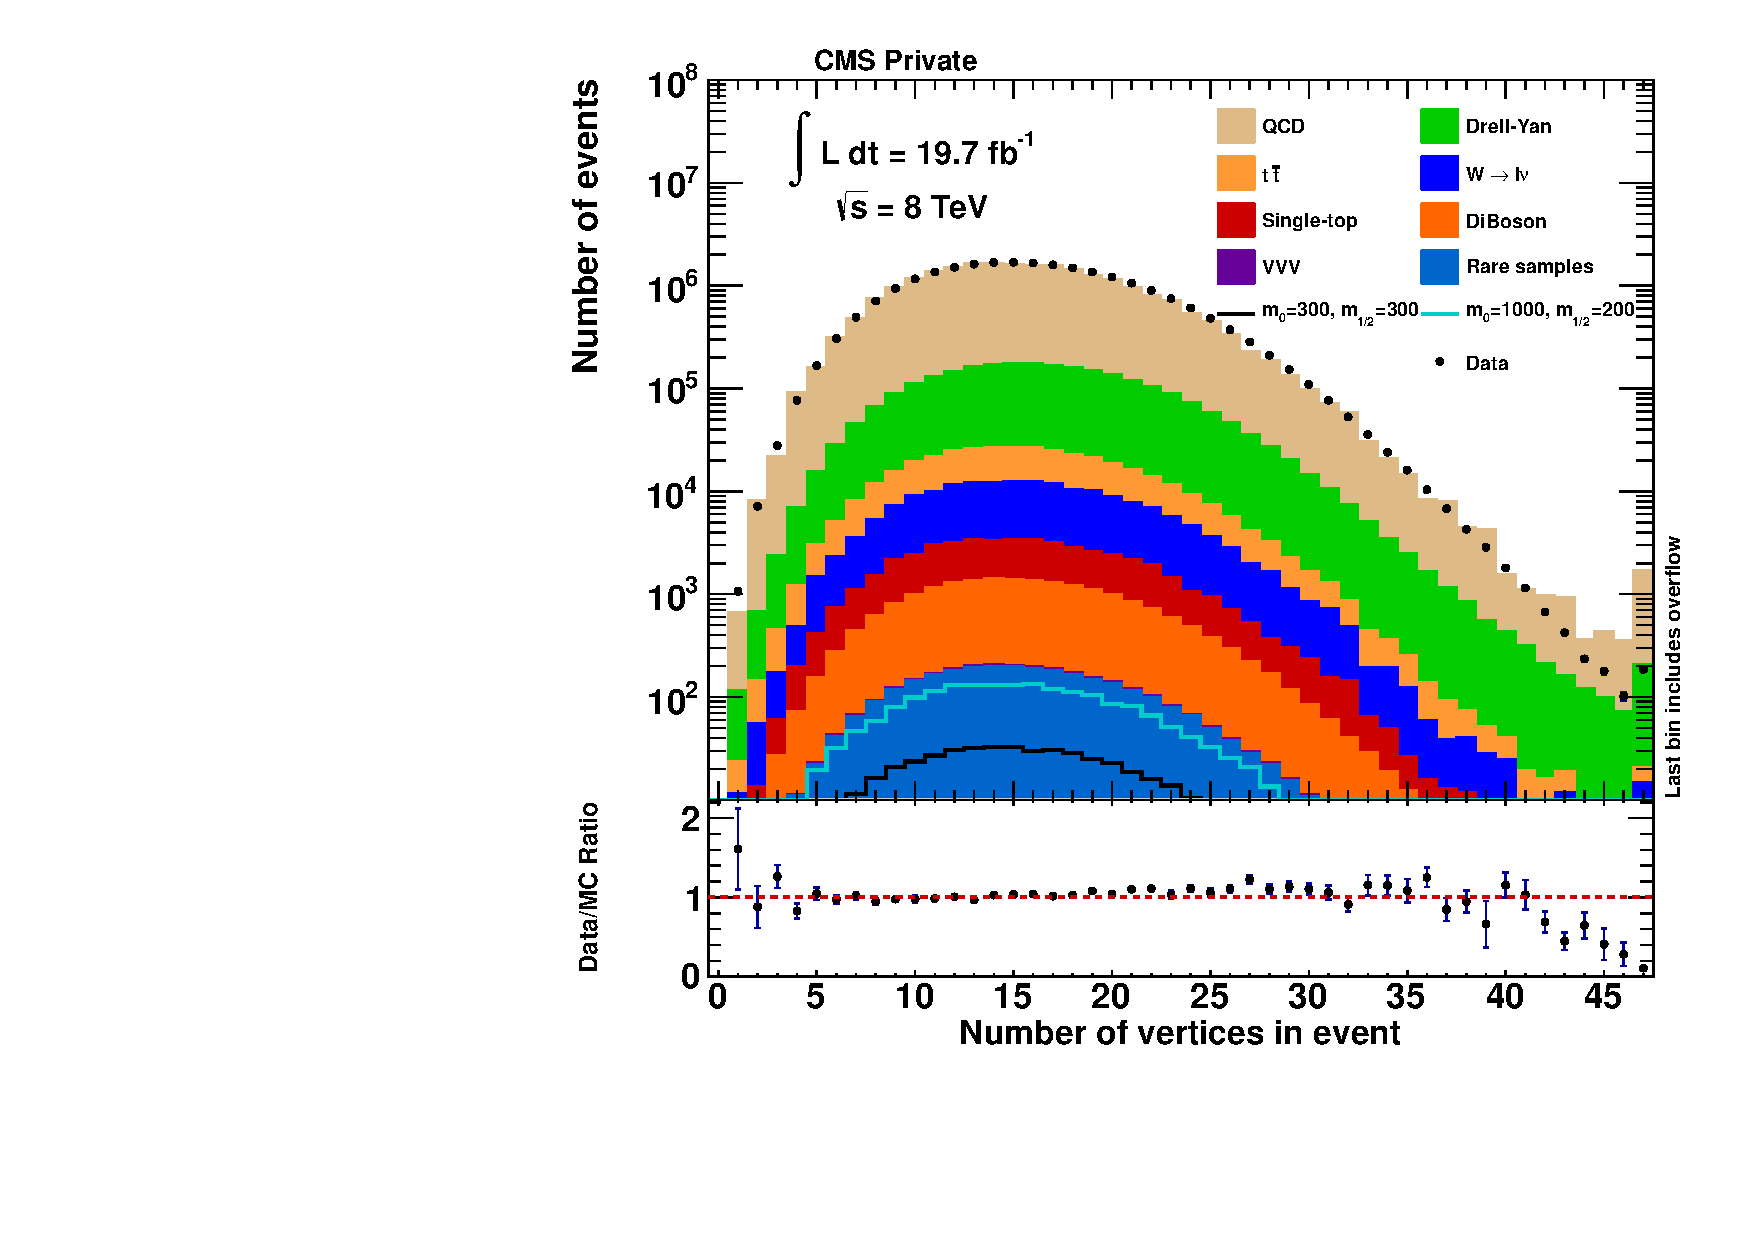
\includegraphics[width=\textwidth]{plots/vtx_n.pdf}
    \caption{\label{fig:vtx_n}}
  \end{subfigure}
  \caption{Number of vertices with (\ref{fig:vtx_n}) and without (\ref{fig:vtx_n_nopu}) pile-up corrections.}
  \label{fig:vtxn}
\end{figure}

\noindent The distributions are from an early stage of the analysis and show the number of vertices before (Fig.~\ref{fig:vtx_n_nopu}) and after (Fig.~\ref{fig:vtx_n}) introducing the weights. It is important to note that data and simulation are not expected to be in good agreement yet. Nonetheless the histograms display the necessity of this procedure.   


\subsection{Jet Energy Resolution}
\label{sec:jer}

With two jets and no missing transverse energy in the final state, the hadronic calorimeter contributes vital information. However, similarly to the pileup situation, the conditions of the simulation differ from the actual measurement. The energy resolution of the calorimeter has been overestimated in the detector simulation. To gain access to the resolution, the objects after the simulation stage can be compared to the generator-level ones. Based on this information and the a set of measurements the necessary scale factor can determined.

Every reconstructed particle flow jet above $15\,\text{GeV}$ transverse momentum is considered relevant for the analysis. The algorithm searches a cone of $\Delta R = \sqrt{\Delta\phi^2 + \Delta\eta^2} = 0.5$ in spatial distance around each reconstructed (\textbf{reco-}) jet. It adds up the transverse momentum of generator-level (\textbf{gen-}) jets found within that area. Depending on whether or not any objects are found, a different recipe for adjusting the jet energy resolution (\textbf{JER}) has to be used.

\begin{itemize}
\item \textbf{Matched gen-jets:} In this case the following formula is used to smear the jet energy.
  \begin{equation}
    \label{eq:jermatched}
    p^\prime_{\text{T}} = p_{\text{T}, \text{GEN}} + c \cdot (p_{\text{T}} - p_{\text{T}, \text{GEN}})
  \end{equation}
  
  \noindent Here $c$ denotes the core resolution scaling factors. To determine those, $0.8\,\text{fb}^{-1}$ of 2011 dijet data\footnote{No significant deviations have been observed with more statistics and 2012 data} has been used. The values are given in table~\ref{tab:jerfactors}.

  \begin{table}[htbp!]
    \centering
    {\renewcommand{\arraystretch}{1.2}
      \begin{tabular}{|c|c|}
        \hline
        $\eta$-Range & Ratio of data/MC $\pm$ stat. $\pm$ sys. \\ \hline \hline
        $0.0 < \eta < 0.5$ & $1.052 \pm 0.012 ^{+0.062}_{-0.061}$ \\ \hline
        $0.5 < \eta < 1.1$ & $1.057 \pm 0.012 ^{+0.056}_{-0.055}$ \\ \hline
        $1.1 < \eta < 1.7$ & $1.096 \pm 0.017 ^{+0.063}_{-0.062}$ \\ \hline
        $1.7 < \eta < 2.3$ & $1.134 \pm 0.035 ^{+0.087}_{-0.085}$ \\ \hline
        $2.3 < \eta < 5.0$ & $1.288 \pm 0.127 ^{+0.155}_{-0.153}$ \\ \hline
      \end{tabular}
    }
    \caption{Core resolution scaling factors for jet energy smearing. They are taken from the JER TWiki~\cite{jer}.}
    \label{tab:jerfactors}
  \end{table}
  
\item \textbf{No matched gen-jets:} Without a gen-jet match the jet energy resolution cannot be estimated. As an alternative method, one can randomly smear the \textit{reconstructed} transverse momentum of the jet. The values are assumed to follow a Gaussian distribution with a width of $\sigma = \sqrt{c^2-1} \cdot \sigma_{\text{MC}}$. The core resolution scaling factors $c$ remain the same, but the energy resolution of jets $\sigma_{\text{MC}}$ has to be derived from the Monte Carlo samples. In figure~\ref{fig:jerdeltapt} the difference between the transverse momentum of matched reco- and gen-jets is shown.

  \begin{figure}[htb!]
    \centering
    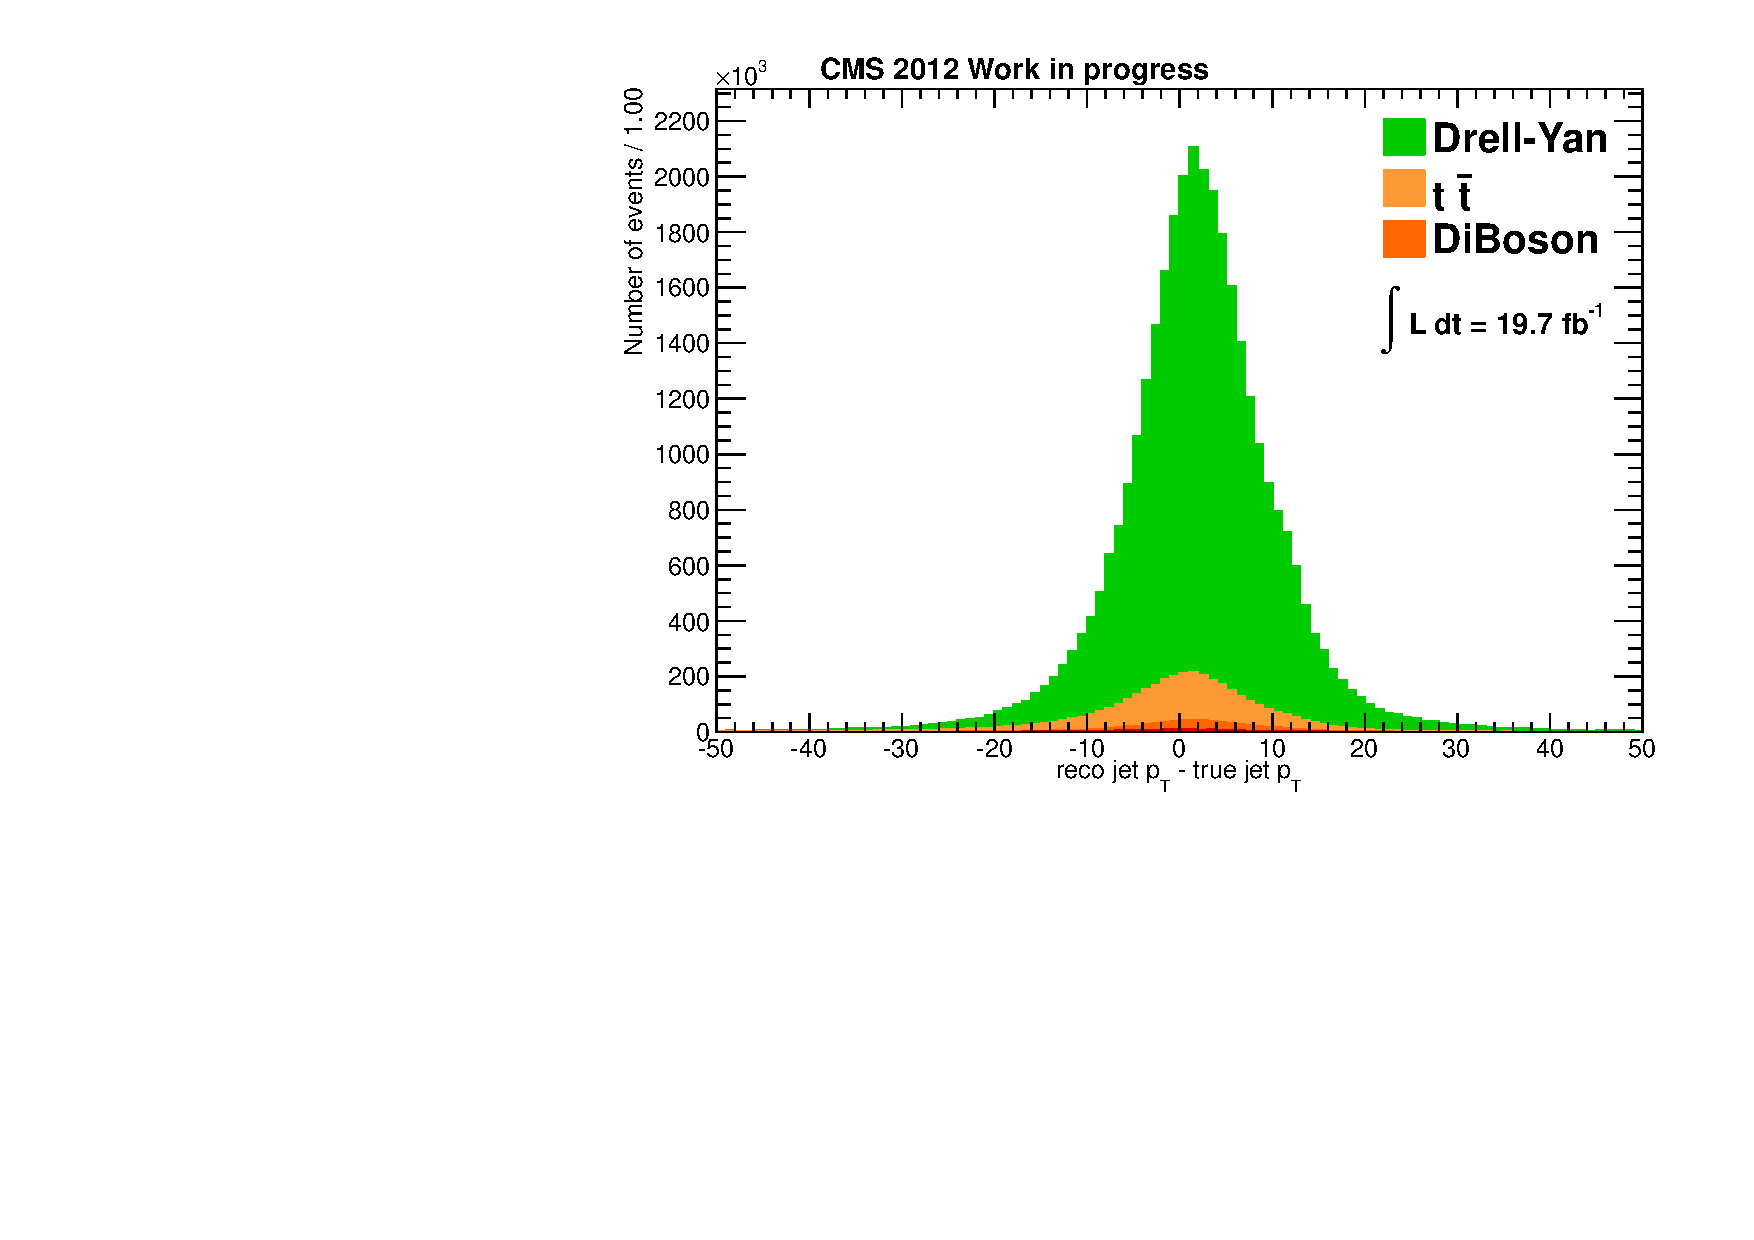
\includegraphics[width=0.6\textwidth]{plots/jer_deltapt.pdf}
    \caption{Difference of transverse momenta from matched reco- and gen-jets in a $\Delta R = 0.5$ cone. This is used to determine the jet energy resolution.}
    \label{fig:jerdeltapt}
  \end{figure}
 
  \noindent Determining the width of this distribution yields the energy resolution. The shape cannot be accurately described by any commonly known distributions, however the width is reasonably well described by a Gaussian function. It yields $\sigma_{\text{MC}} = 7.32$ with an negligible statistical error, which is one order of magnitude lower than the last significant digit. Keeping the shape in mind, the systematic uncertainty of the fit is expected to be higher. Thus the given precision is a conservative estimate.
\end{itemize}

The correction to the transverse momenta is propagated to the directional momenta, energy and the missing transverse energy measurements. In figure~\ref{fig:jermet} the particle flow missing transverse energy is shown with and without the correction. Due to the adjustment being expected to be comparatively small, the histogram has been filled at a later stage of the analysis. This ensures a reasonable agreement between data and simulation prior to examining the effect of the jet energy resolution.

\begin{figure}[htb!]
  \centering
  \begin{subfigure}[b]{0.495\textwidth}
    \centering
    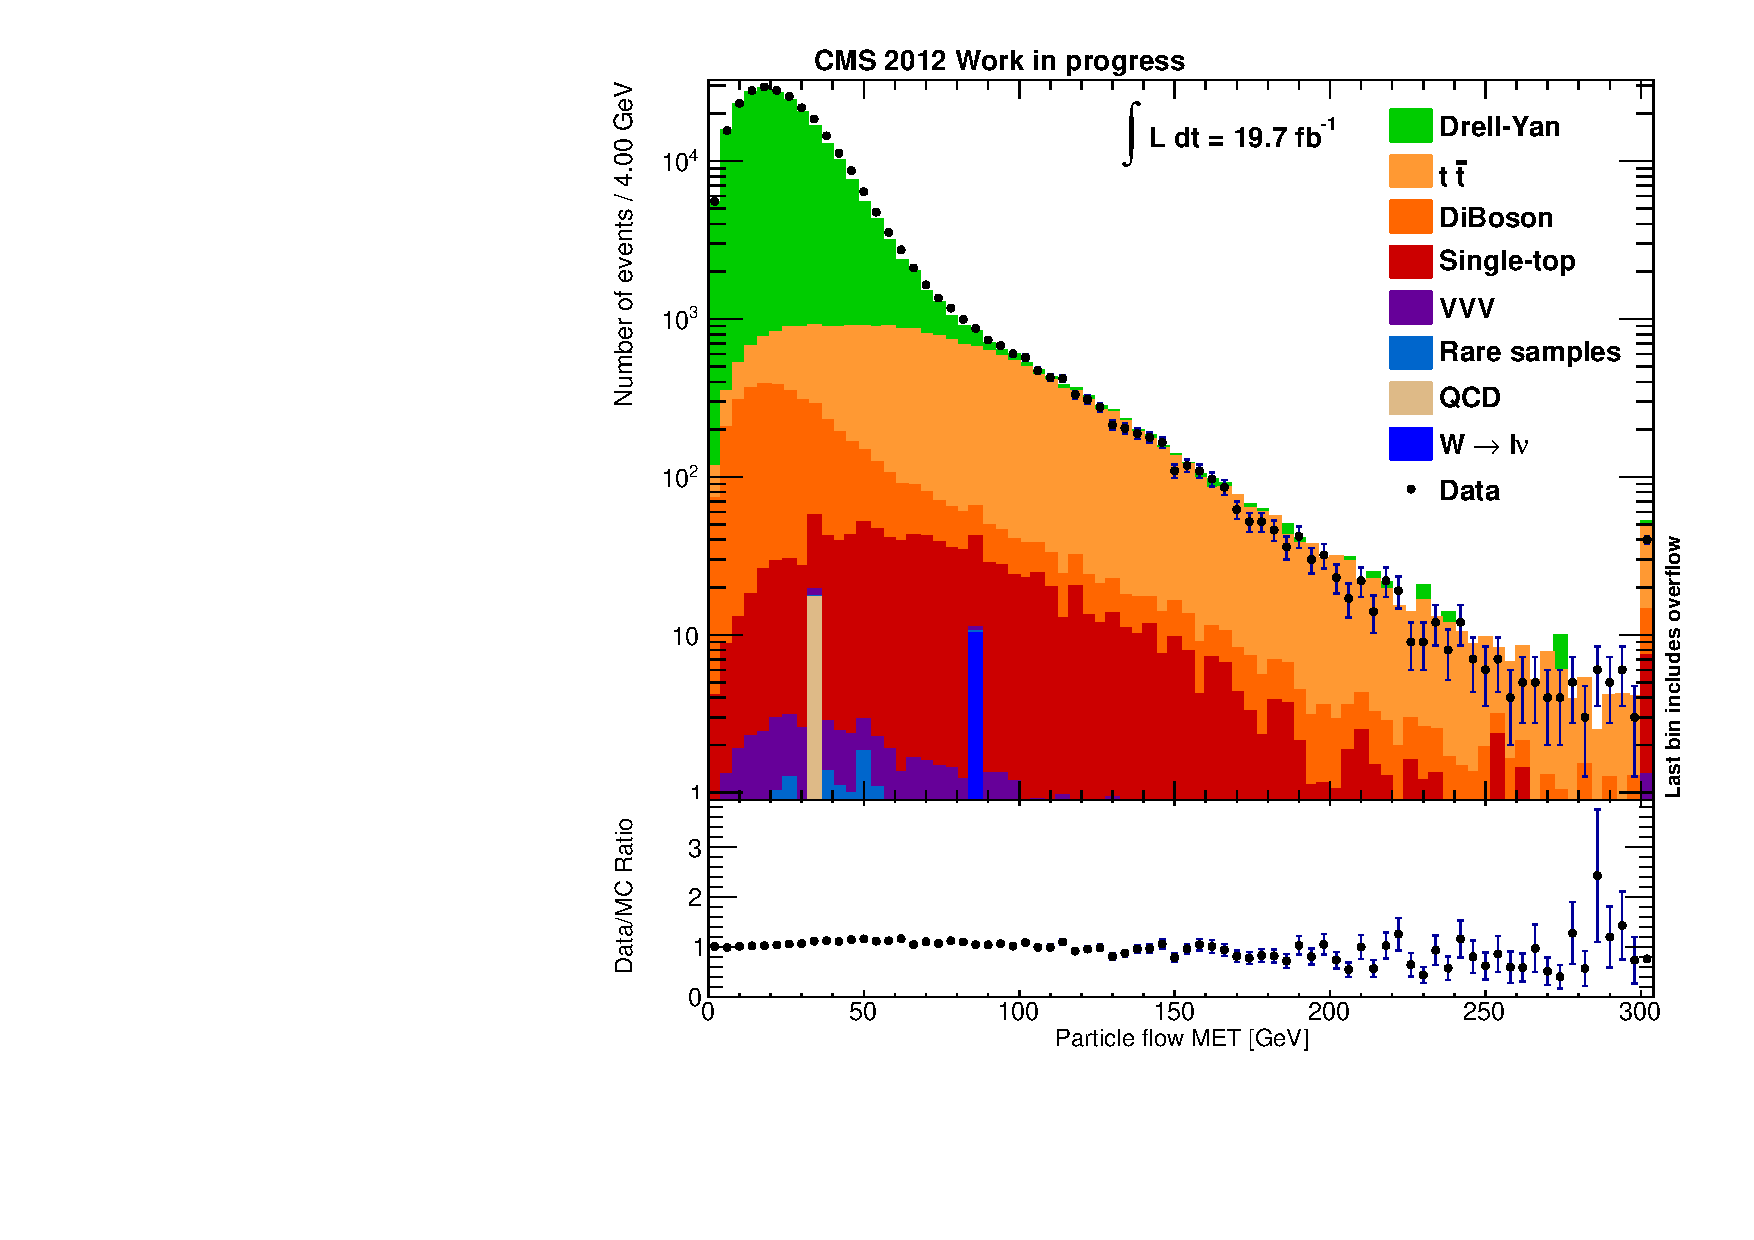
\includegraphics[width=\textwidth]{plots/pfmet_nojer.pdf}
    \caption{\label{fig:jerpfmet_nojer}}
  \end{subfigure}
  \begin{subfigure}[b]{0.495\textwidth}
    \centering
    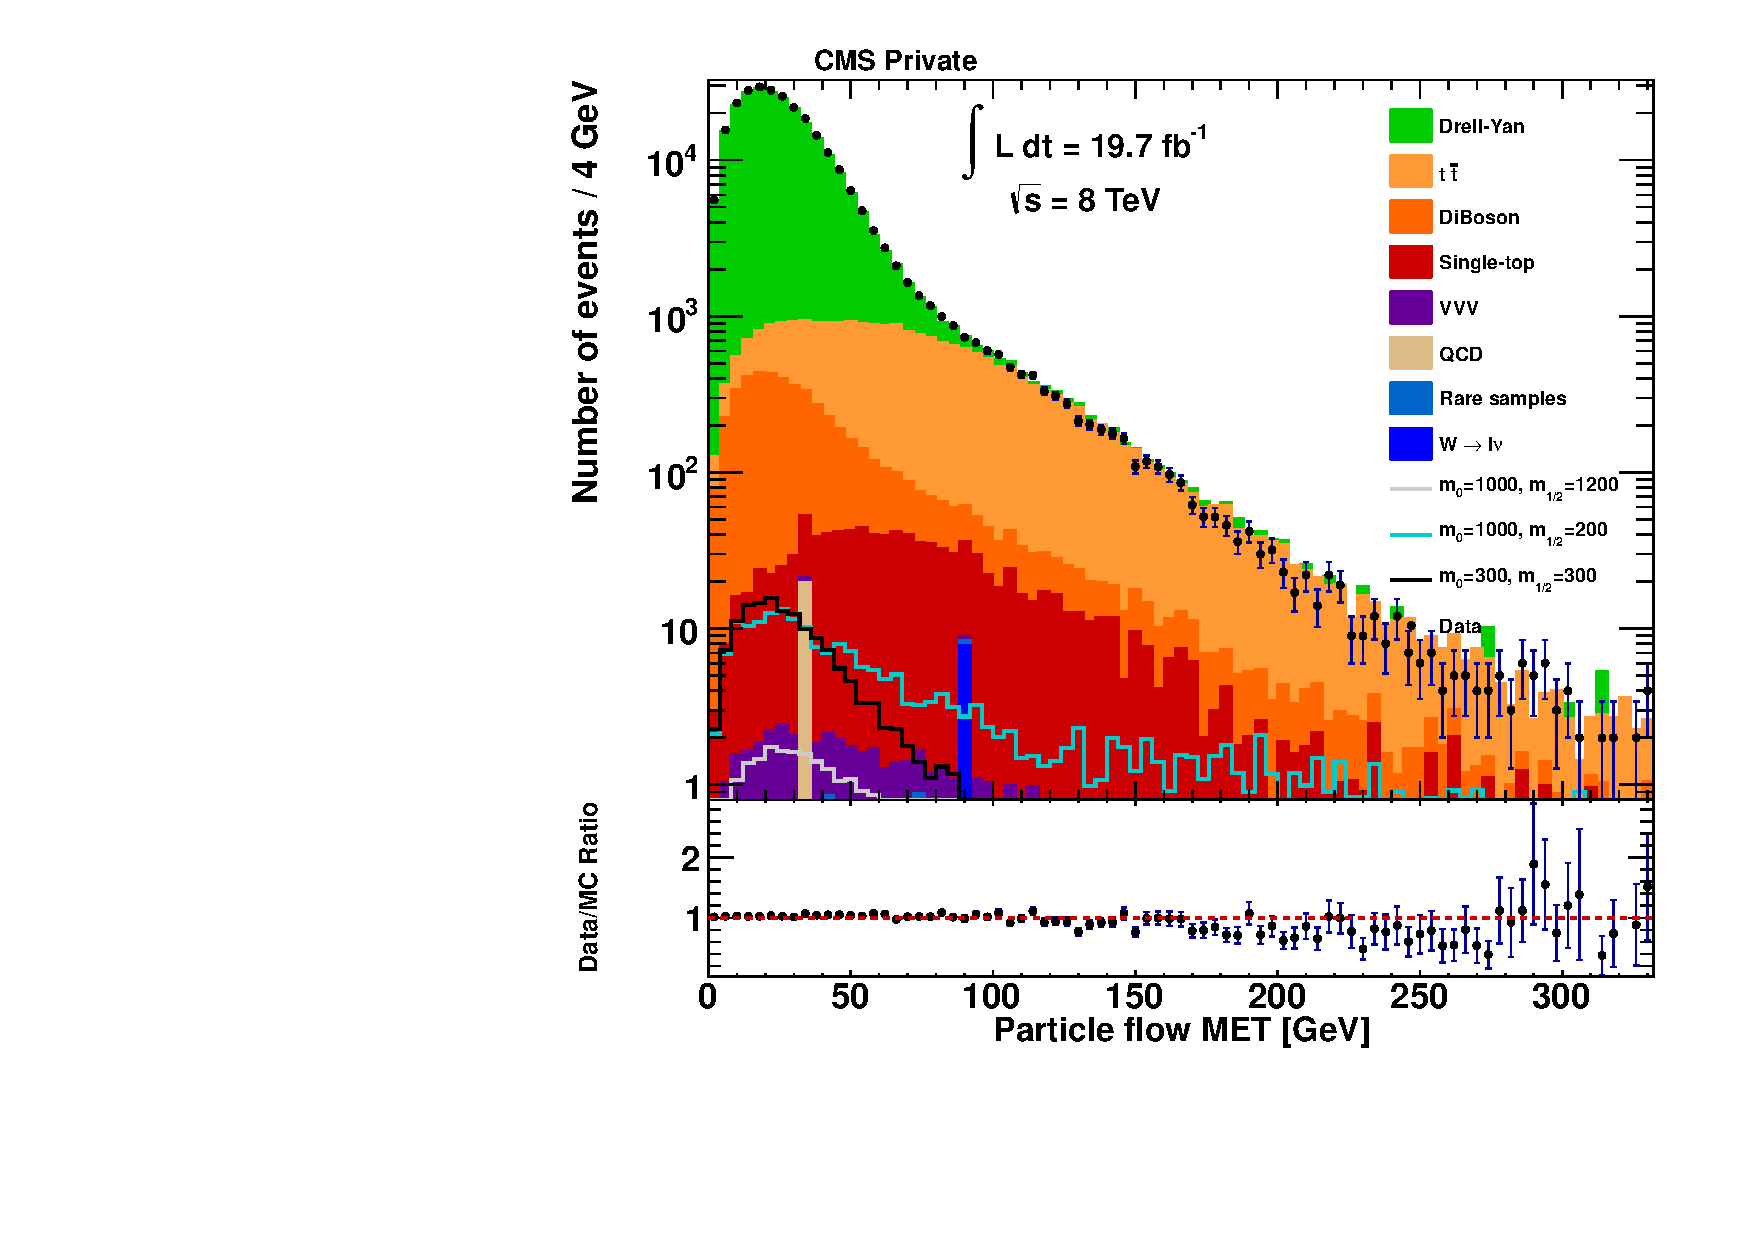
\includegraphics[width=\textwidth]{plots/pfmet.pdf}
    \caption{\label{fig:jerpfmet}}
  \end{subfigure}
  \caption{Particle flow missing transverse energy with (\ref{fig:jerpfmet}) and without jet energy corrections (\ref{fig:jerpfmet_nojer}).}
  \label{fig:jermet}
\end{figure}

\noindent One can observe a small, but still noticeable improvement due to the correction. This is best visible on the right flank of the distribution, where the Drell-Yan process still dominates. 


%%% Local Variables: 
%%% mode: latex
%%% TeX-master: "document"
%%% End: 

\chapter{Object Selection}
\label{cha:objsel}

Choosing recipes for selecting well reconstructed physics objects is necessary before one is able to apply analysis requirements. Their general task is to reduce the number of false reconstructions. For example a hadron can ``punch through'' the HCAL and leave a track in the muon system. This might then be falsely identified as a muon and interfere with the signal. These recipes for object identification (\textbf{ID}) have been developed by the respective physics object groups (\textbf{POG}). In this chapter, the various steps in the decision of deeming an object valid or invalid will be given.

\section{Triggers}
\label{sec:trigger}

Before selecting physics objects, a trigger has to be chosen. Although DoubleMu datasets already necessitate dimuon triggers, only a selected few are well suited for the specified signature. A primary concern is a low trigger prescale. Prescaling means that the amount of events passing the trigger is suppressed by a certain factor to control its rate (and the amount of data manageable). To be able to allow for a low prescale factor, the requirements for each trigger have to be strict enough. Usually the transverse momentum threshold for the object can be raised to ensure an acceptable rate of events, but keeping the essentially prompt decay in mind, another option is available. Various triggers have a $|\Delta z_{\mu\mu}| < 0.2\,\text{cm}$ requirement, filtering out events with a large distance in the $z$-direction between the muon-pair. This effectively enables the inclusion of the low momentum regions in the search. The remaining options for high level triggers are:

\begin{itemize}
\item \verb+HLT_Mu17_Mu8+
\item \verb+HLT_Mu17_TkMu8+
\end{itemize}

Both have an HLT prescale of 1 and are the triggers with the lowest available transverse momentum threshold given by the numbers in their names. With an identical requirement for the primary muon, the major difference is the reconstruction of the second muon. The first trigger path requires both muons to be global ones, while in the other path the second muon only needs to be a tracker muon. As already discussed in the object reconstruction (Sec.~\ref{sec:objreco}), the latter can allow events with two collimated muons to pass which would otherwise be discarded.

To quantify the difference between both triggers, the number of selected events can be compared. In figure~\ref{fig:matched} the number of data events passing various combinations of the two triggers are shown.

\begin{figure}[ht!]
  \centering
    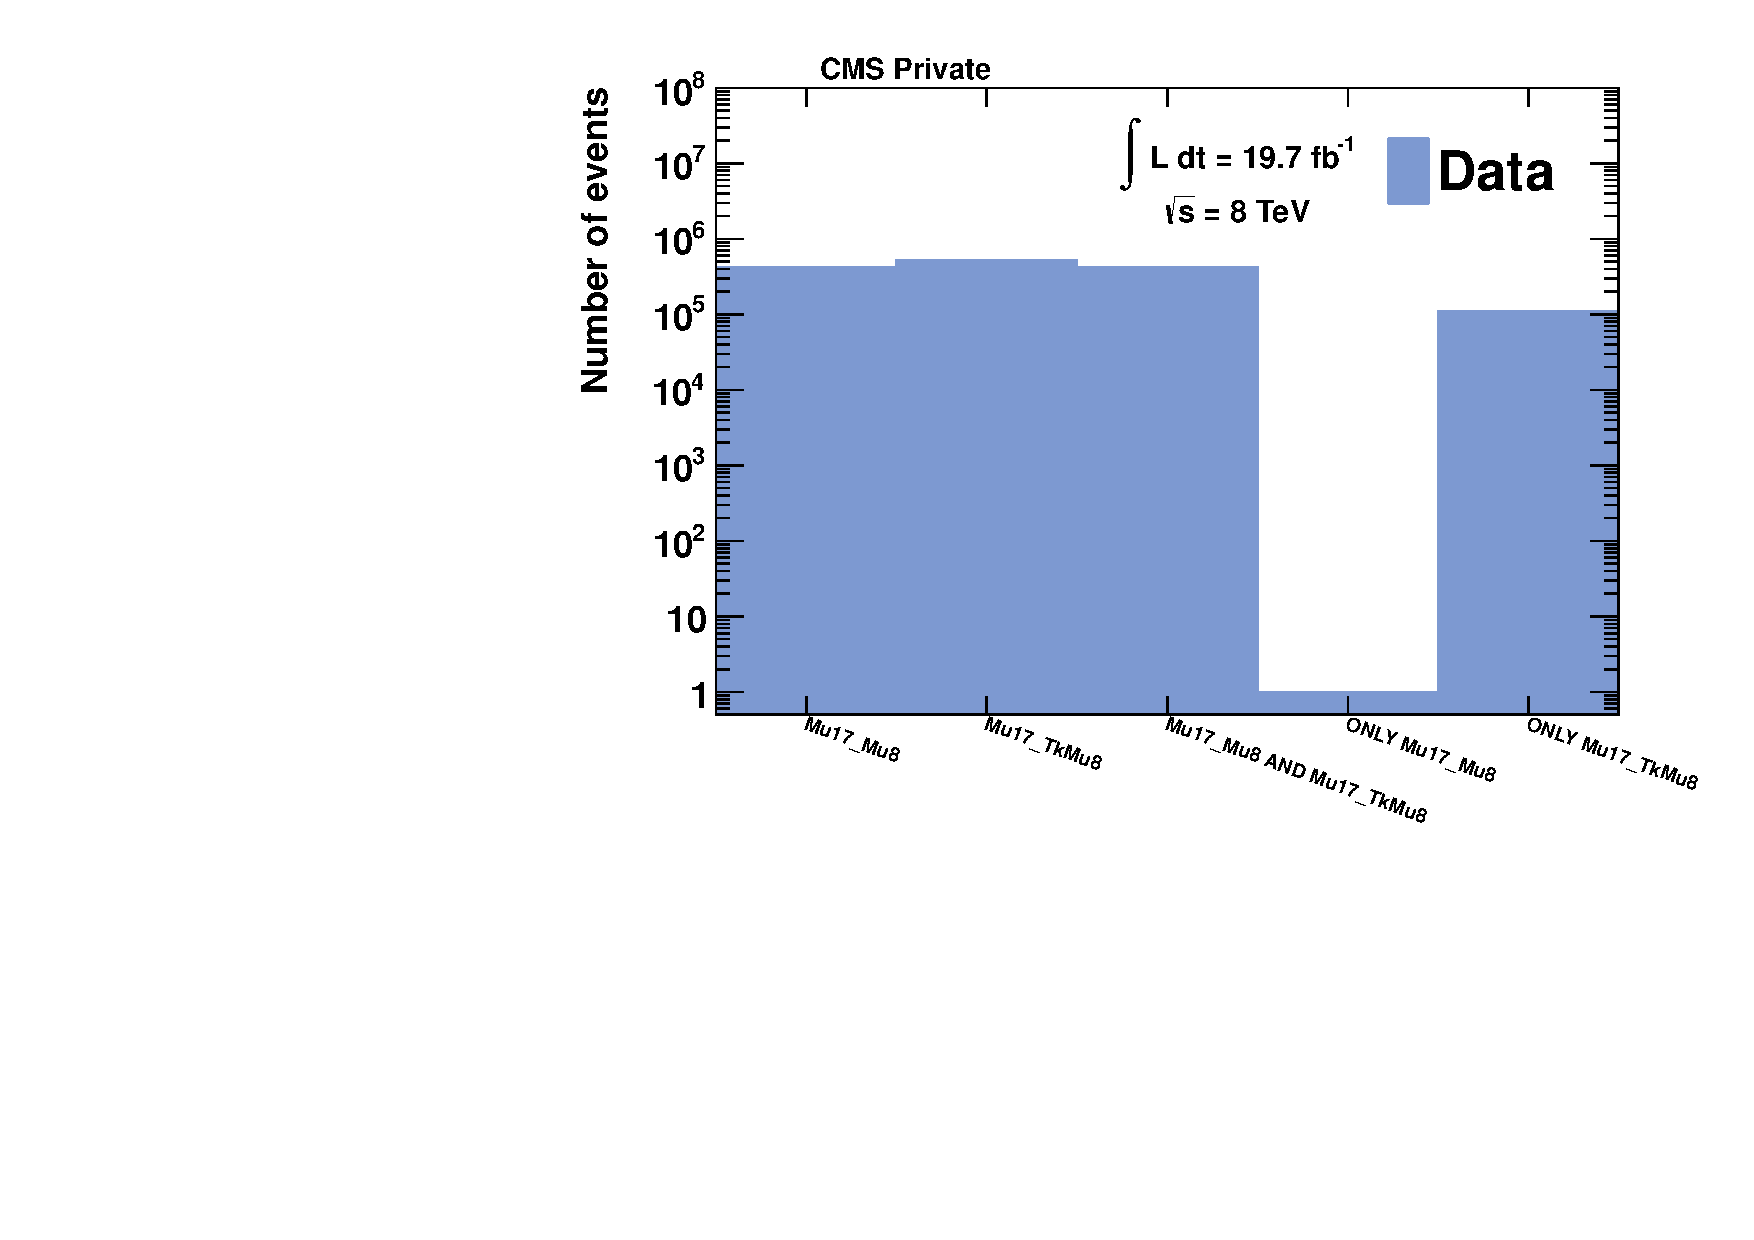
\includegraphics[width=0.8\textwidth]{plots/dycut_matched.pdf}
  \caption{Each bin represents the number of data events passing the various trigger combinations given on the $x$-axis. All four runs of 2012 (Tab.~\ref{tab:data}) are included in this distribution.}
  \label{fig:matched}
\end{figure}

\noindent The first two bins of the distribution show the results for each individual trigger. By raw numbers, \verb+HLT_Mu17_TkMu8+ is in the lead in terms of overall efficiency. To get en estimate of the overlap, the third bin shows the case when both triggers are required at once. With the number of events being quite similar to the one for \verb+HLT_Mu17_Mu8+, one can conclude that almost all events in the first bin are contained in the second one as well. To further quantify this conclusion, the fourth and fifth bin display the event count of \textit{only} one out of the two being triggered. Comparing the contents of these bins with the previous ones, the additional efficiency yielded by using \verb+HLT_Mu17_Mu8+ in addition to \verb+HLT_Mu17_TkMu8+ can be estimated. With it being only of the order of $\mathcal{O}(10^{-5})$, this analysis uses the latter trigger exclusively.


\section{Muon Identification}
\label{sec:muonid}

The recipe employed for muon identification has been developed by the Muon POG. The current recommendations can be found on the respective TWiki Website~\cite{muonpog}. Its main purpose is to differentiate between prompt and non-prompt muons.

Since the analysis expects a low amount of statistics in the final distributions, the tight muon ID~\cite{muonid1, muonid2} has been chosen. This is the most strict criterion given by the physics object group, thus being the best choice to prevent misidentification. The requirements are given below and apply to all muons within the intermediate energy range.

\begin{itemize}
\item \textbf{Global Muon} - The object is required to be identified as global muon. As discussed in the object reconstruction (Sec.~\ref{sec:objreco}), this means that a set of hits in the muon system has to be matched to a compatible set in the tracker. With mostly muons being able to pass through the inner detector layers, this serves as a major tool for identifying muons.
\item \textbf{Particle Flow Muon} - As outlined in the object reconstruction, particle flow algorithm considers the measurements from all sub-detectors. By combining the information of an entire event, the accuracy of particle identification is improved.
\item \textbf{Muon Track} $\mathbf{\chi^2 / N_{\textbf{dof}} < 10}$ - The fit of the trajectory has to describe the hits reasonably well. This is meant to protect against muons stemming from a decay in flight, as well as hadron passing the HCAL~\cite{muonidcosmic}. In both cases the trajectory is likely not to have a good match in the tracker region.
\item $\mathbf{N_{\textbf{Muon Chambers}} > 0}$ - For the same purpose at least one muon chamber has to be part of the global fit. 
\item $\mathbf{N_{\textbf{Matched Stations}} > 1}$ - Requiring at least two muon stations to have a muon segment hit provides consistency with the trigger\footnote{A reasonable estimate for the transverse momentum requires a minimum of three hits. Without a well reconstructed transverse momentum, the trigger threshold becomes meaningless as it is based upon that.}. Once again, this aids against punch-through particles and also against general mismatches of tracks.
\item $\mathbf{|d_{xy}| < 2\,\textbf{mm}}$ - The impact parameter in the transverse plane, in respect to the primary vertex\footnote{The primary vertex is defined as the vertex with the largest sum of squared transverse track momenta in an event.}, has to be low. Both decays in flight and cosmic muons are unlikely to meet this criterion~\cite{muonidcosmic}.
\item $\mathbf{|d_z| < 5\,\textbf{mm}}$ - The longitudinal distance towards the primary vertex also has to be low for the same reasons.
\item $\mathbf{N_{\textbf{Pixel Hits}} > 0}$ - Since in flight decays may not have hits in the pixel detector, this requirement provides further suppression and association to a single vertex.
\item $\mathbf{N_{\textbf{Tracker Layers}} > 0}$ - A certain amount of tracker CSC layers needs to be hit for a precise transverse momentum measurement. Additionally, the same logic as for the hits in the pixel detector applies.
\end{itemize}

The detector coverage only ensure a consistent momentum resolution for muons in the $\eta$-region up to 2.1 (Cf. cha.~\ref{cha:experiment}). Hence the analysis limits itself to this region. Together with a minimum transverse momentum set by the trigger, these are the basic criteria for object selection with regards to muons. They will be used and expanded upon in the event selection (Sec.~\ref{cha:eventsel}).

Additional distributions displaying the effects of the individual ID criteria can be seen in figure~\ref{fig:n-1}. To be able to visualize the individual impact of a requirement from a given recipe, the histogram is only filled with events passing all of the recipe's requirements excluding the one to be examined. These so-called ``N$ - 1$ plots'' show the parameter regions which are \textit{only} excluded because of the requirement in question.

\begin{figure}[!htbp]
  \centering
  \begin{subfigure}[b]{0.495\textwidth}
    \centering
    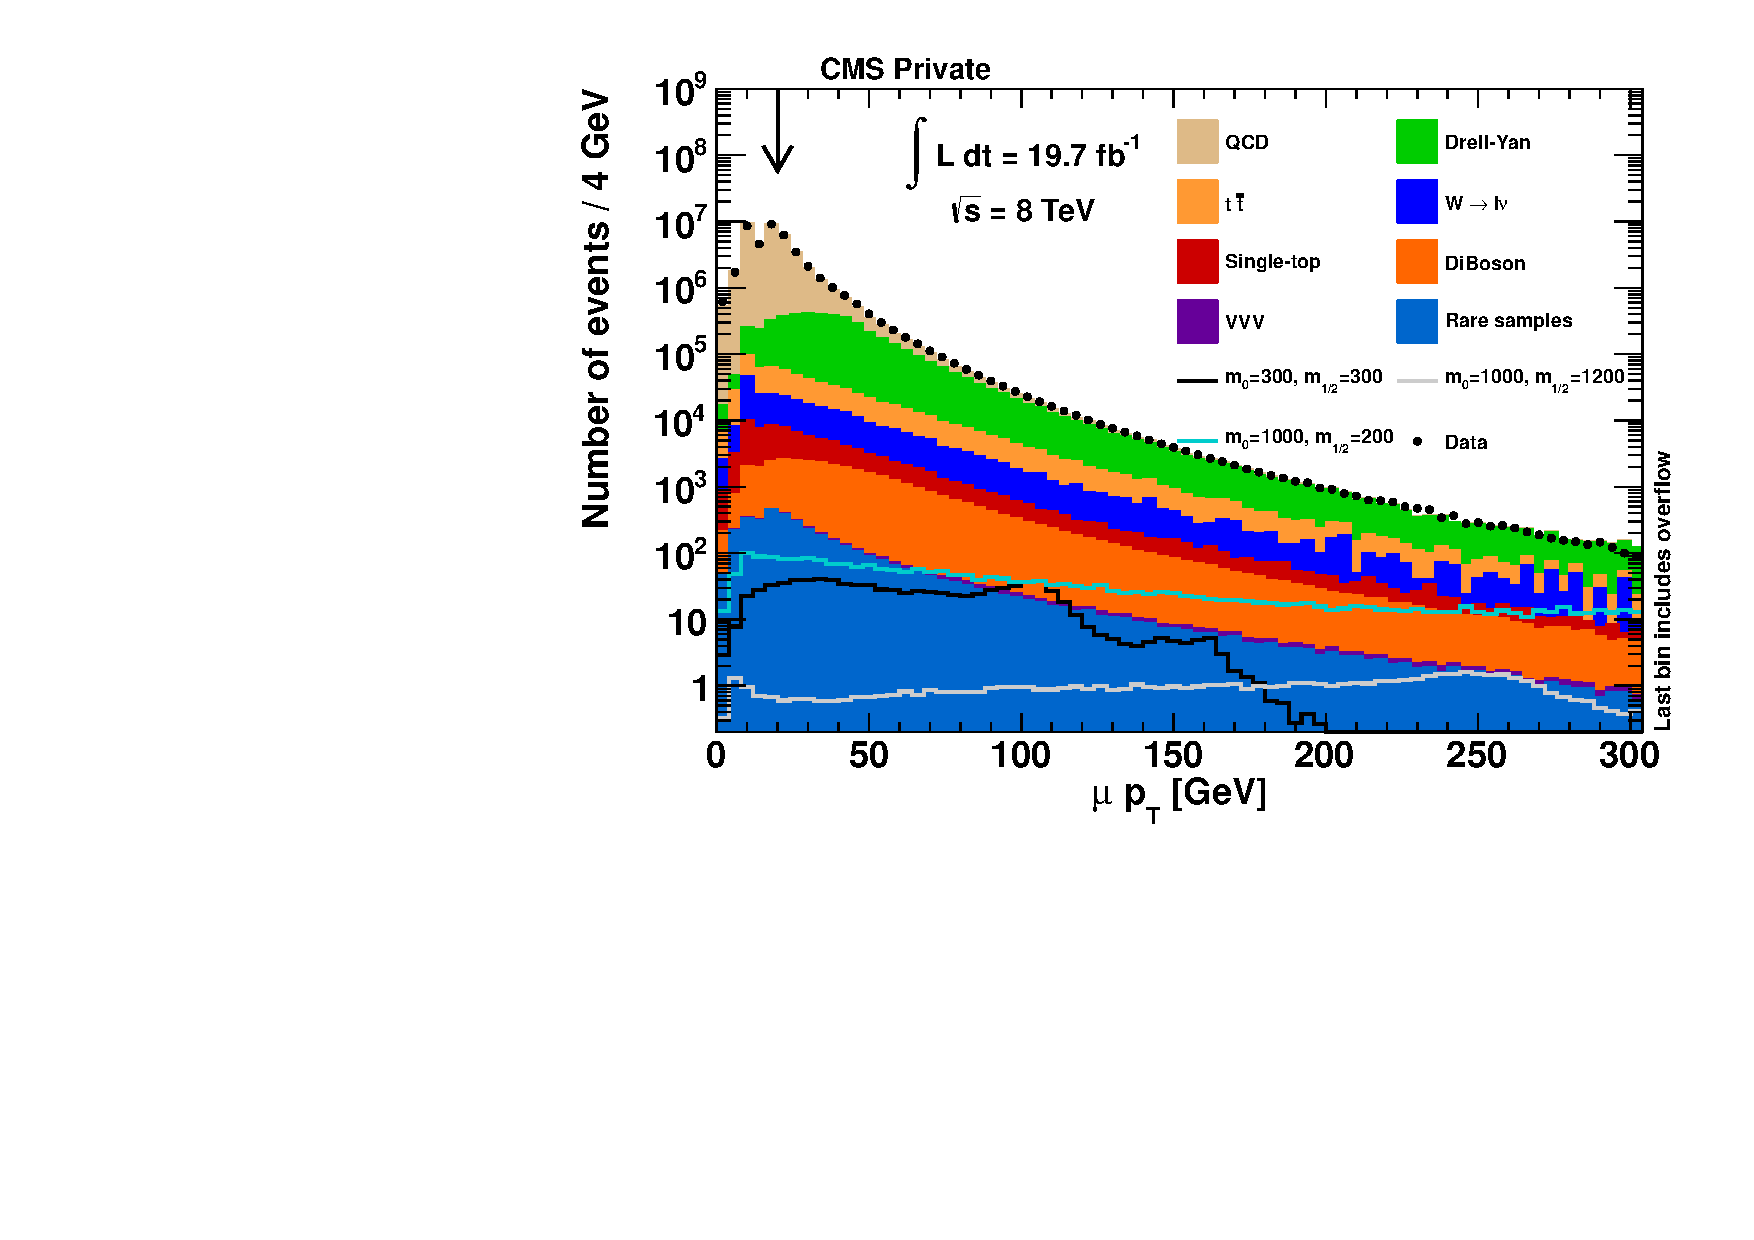
\includegraphics[width=\textwidth]{plots/nMuon_pt.pdf}
    \caption{Transverse momentum of muons\label{fig:muo_pt}}
  \end{subfigure}
  \begin{subfigure}[b]{0.495\textwidth}
    \centering
    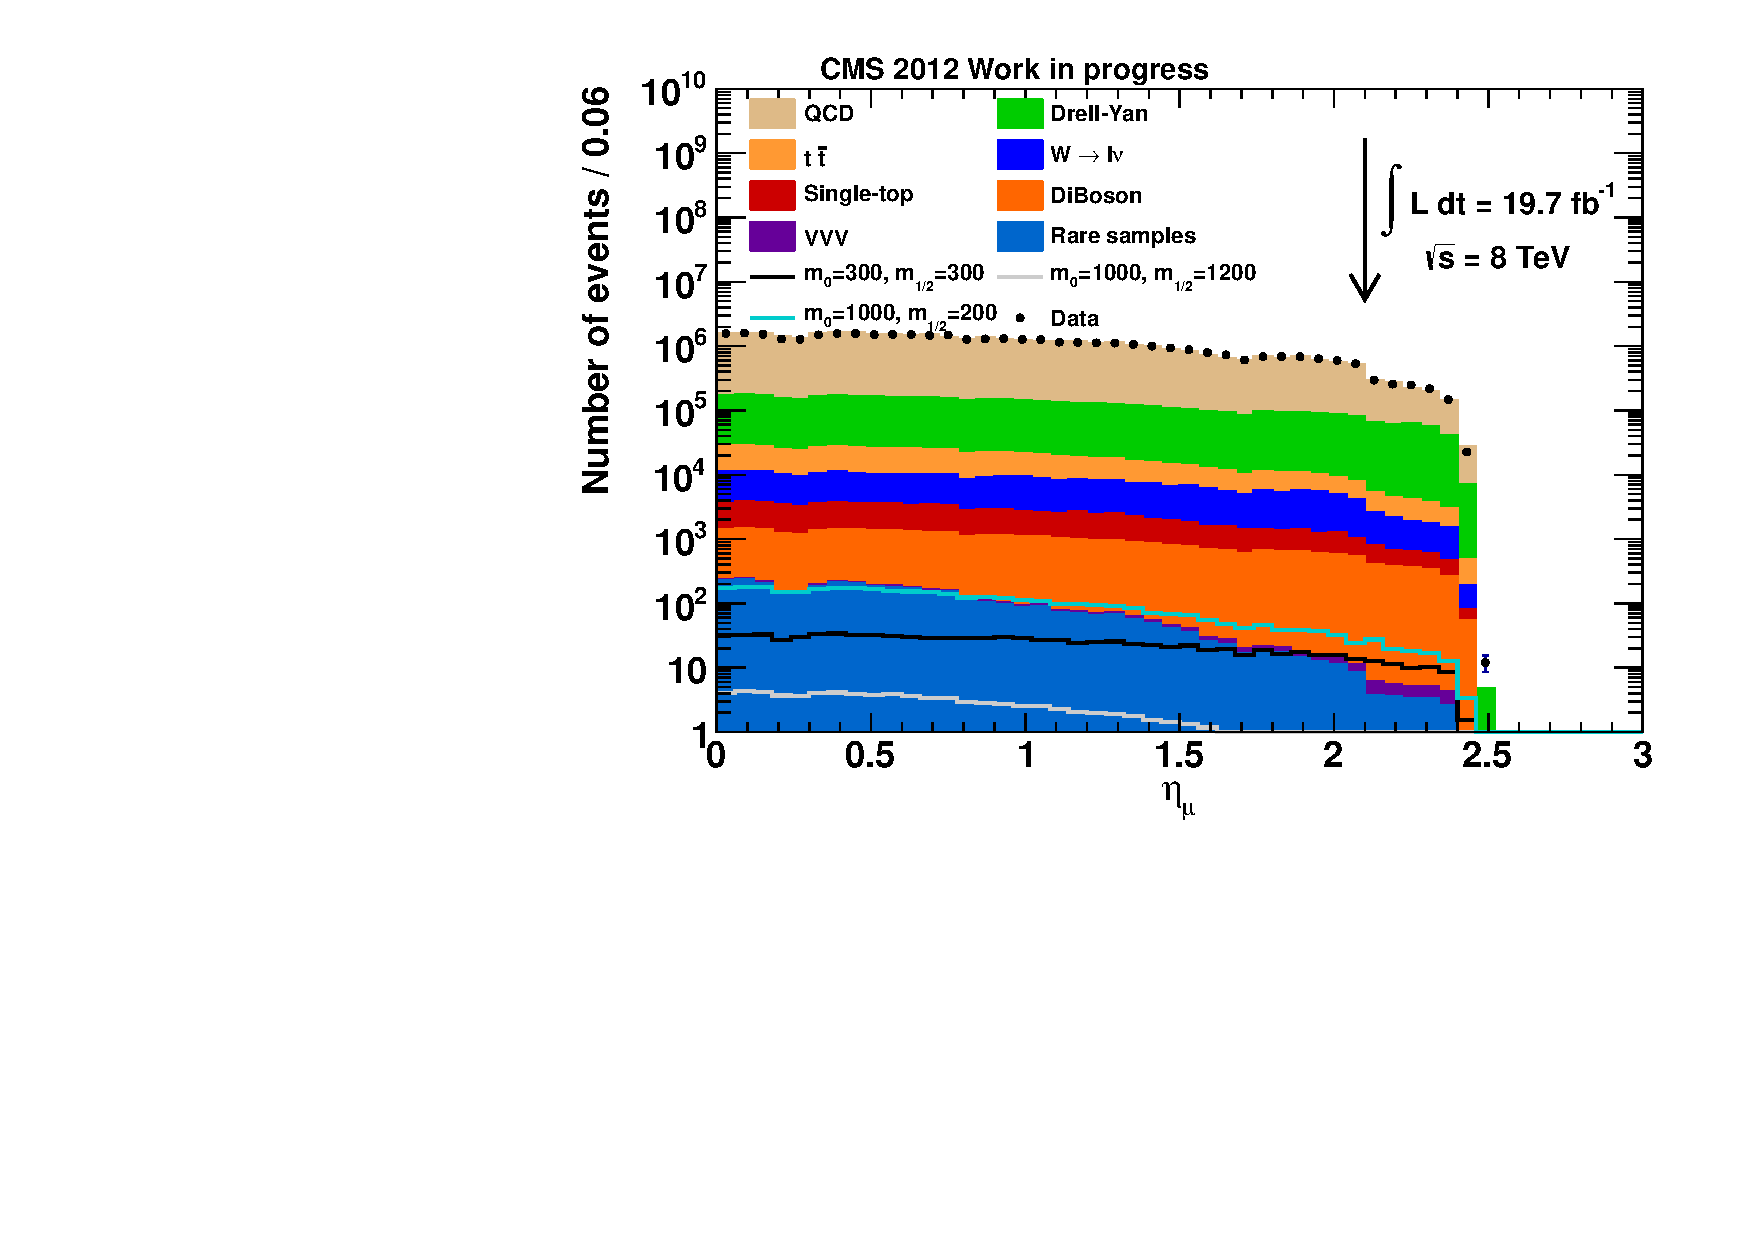
\includegraphics[width=\textwidth]{plots/nMuon_eta.pdf}
    \caption{$\eta$ of muons\label{fig:muo_eta}}
  \end{subfigure}
\end{figure}

\begin{figure}[!htbp]
  \ContinuedFloat
  \centering
  \begin{subfigure}[b]{0.495\textwidth}
    \centering
    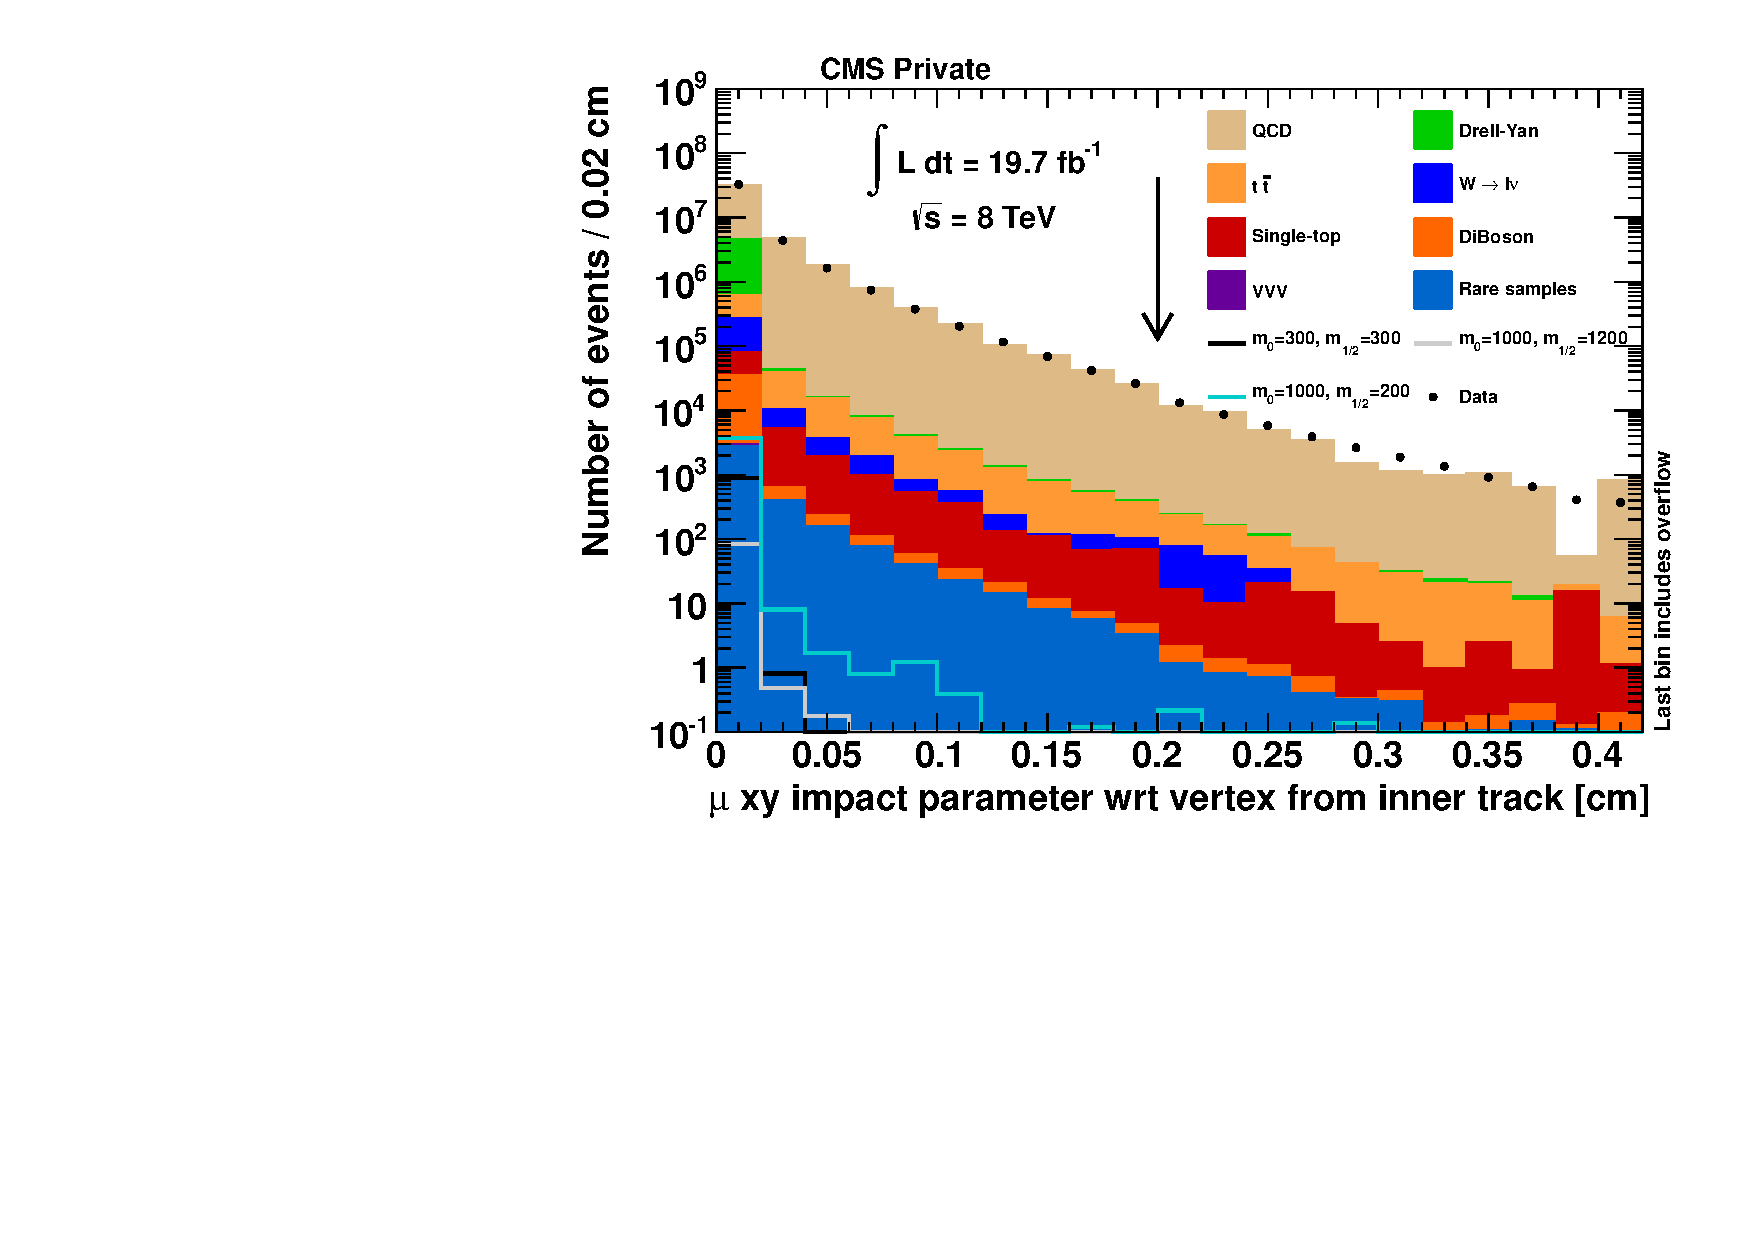
\includegraphics[width=\textwidth]{plots/nMuon_d0Tk.pdf}
    \caption{Transverse impact parameter of muons\label{fig:muo_d0}}
  \end{subfigure}
  \begin{subfigure}[b]{0.495\textwidth}
    \centering
    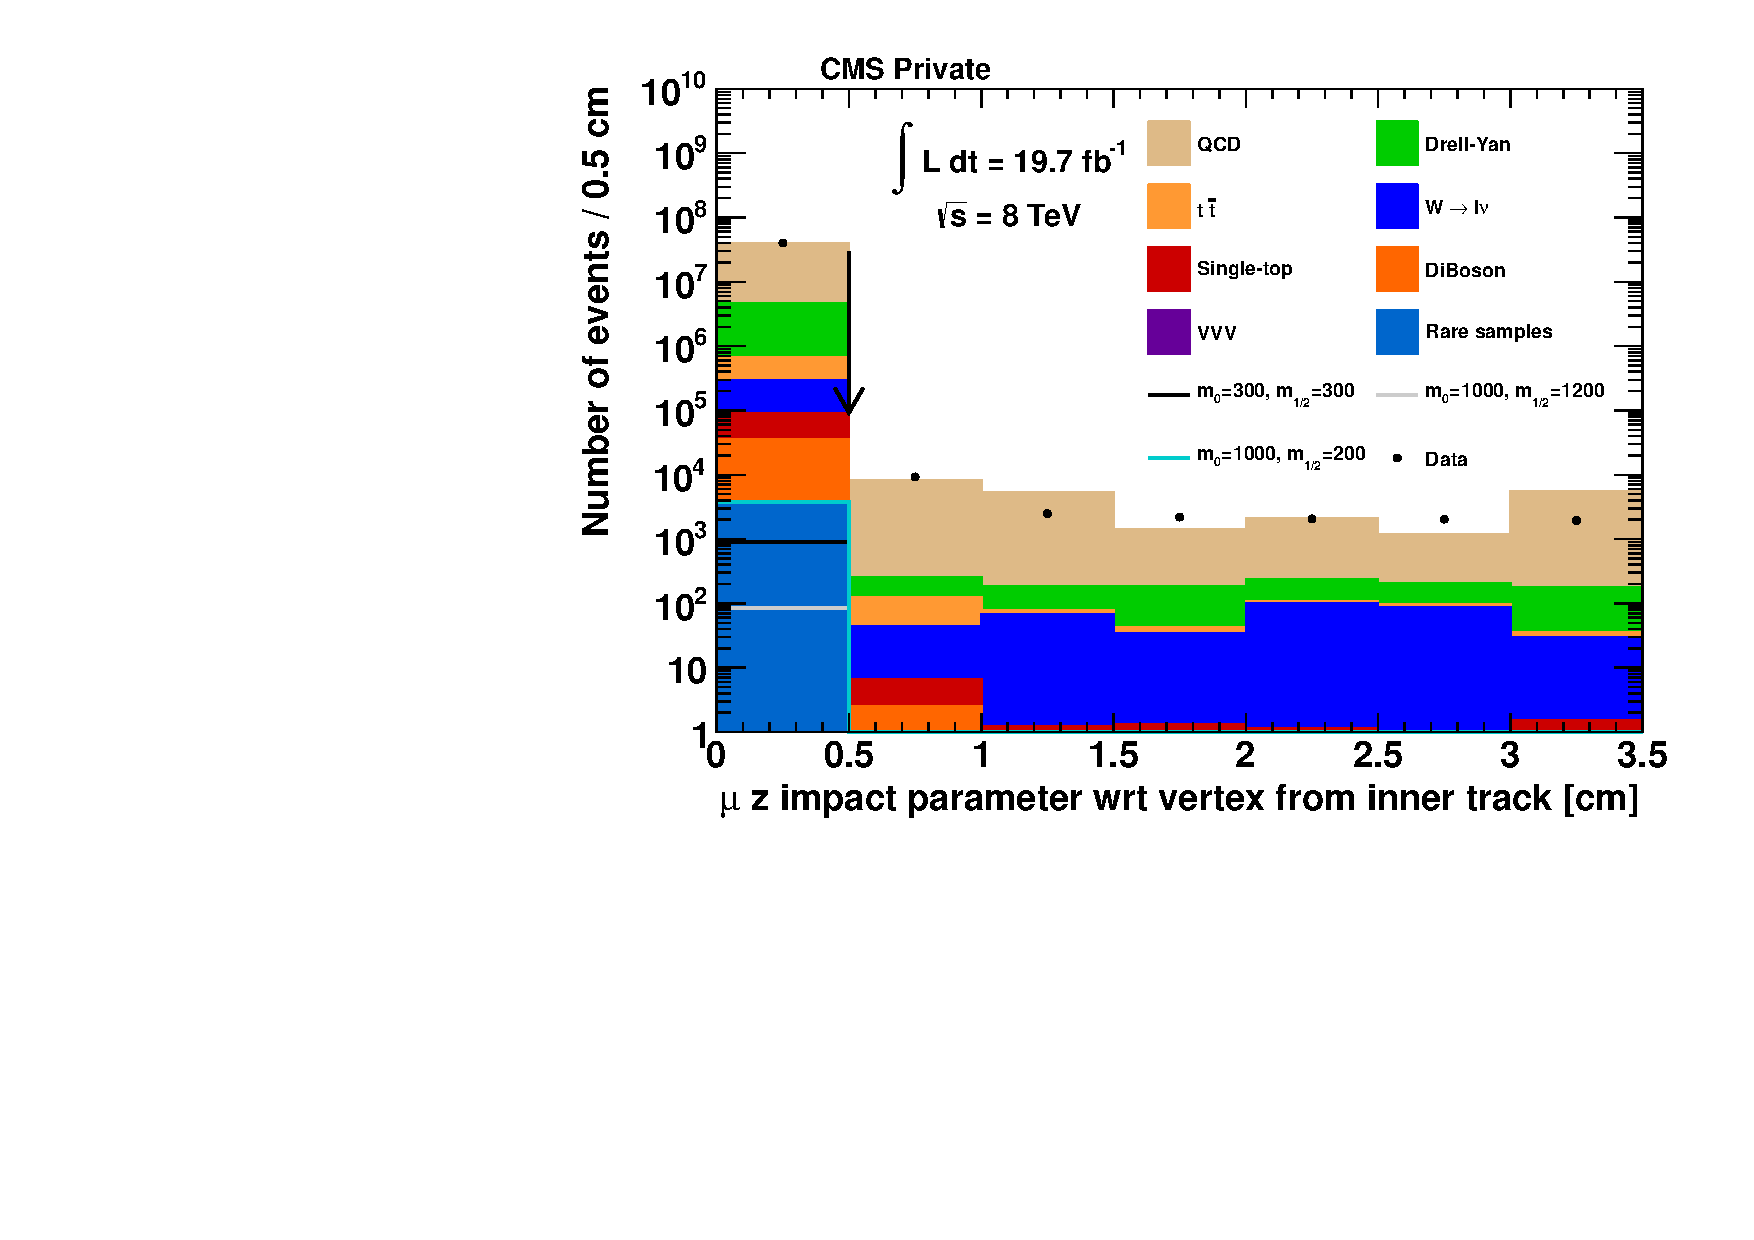
\includegraphics[width=\textwidth]{plots/nMuon_dzTk.pdf}
    \caption{Longitudinal impact parameter of muons\label{fig:muo_dz}}
  \end{subfigure}
\end{figure}

\begin{figure}[!htbp]
  \ContinuedFloat
  \centering
  \begin{subfigure}[b]{0.495\textwidth}
    \centering
    \includegraphics[width=\textwidth]{plots/nMuon_hits.pdf}
    \caption{Combined number of detector hits from muons\label{fig:muo_hits}}
  \end{subfigure}
  \begin{subfigure}[b]{0.495\textwidth}
    \centering
    \includegraphics[width=\textwidth]{plots/nMuon_StationsMatched.pdf}
    \caption{Number of muon stations matched by each muon\label{fig:muo_stationsmatched}}
  \end{subfigure}
\end{figure}

\begin{figure}[!htb]
  \ContinuedFloat
  \centering
  \begin{subfigure}[b]{0.495\textwidth}
    \centering
    \includegraphics[width=\textwidth]{plots/nMuon_ValidPixelHitsCm.pdf}
    \caption{Number of valid hits in the pixel detector by muons\label{fig:muo_validpixelhits}}
  \end{subfigure}
  \begin{subfigure}[b]{0.495\textwidth}
    \centering
    \includegraphics[width=\textwidth]{plots/nMuon_TrkChi.pdf}
    \caption{$\chi^2$ value of the track fitting procedure for muons\label{fig:muo_chi2}}
  \end{subfigure}

  \caption{$n - 1$ distributions of the muon object selection. Requirements are indicated by arrows.}
  \label{fig:n-1}
\end{figure}



\section{Jet \& Missing Transverse Energy Identification}
\label{sec:jetid}

For selecting jets and missing transverse energy, this analysis relies on the work of the JetMET POG~\cite{jmepog}. Jets are reconstructed using the anti-$k_{\text{T}}$ ($\Delta R < 0.5$) and particle flow algorithm. The latter is also responsible for the calculation of the missing transverse energy. The recommended loose working point~\cite{jetid, jetidpf} has been chosen with regards to jet requirements. The idea is to support the event selection which uses muons as its basis, while giving confidence for the final state selection. The values are given below.

\begin{itemize}
\item \textbf{Number Of Constitutents} $\mathbf{> 1}$ - Amount of particle components of the jet.
\item \textbf{Neutral Hadron Fraction} $\mathbf{< 0.99}$ - Fraction of the energy deposited in the HCAL by neutral particles.
\item \textbf{Charged Hadron Fraction} $\mathbf{> 0}$ - Fraction of the energy deposited in the HCAL by charged particles.
\item \textbf{Neutral EM Fraction} $\mathbf{< 0.99}$ - Fraction of the energy deposited in the ECAL by neutral particles.
\item \textbf{Charged EM Fraction} $\mathbf{< 0.99}$ - Fraction of the energy deposited in the ECAL by charged particles.
\item \textbf{Charged Multiplicity} $\mathbf{> 0}$ - Number of charged jet components.
\end{itemize}

For the transverse momentum threshold and spatial coverage $15\,\text{GeV}$ and $|\eta|  < 2.4$ are required. A spatial distance of at least $\Delta R > 0.05$ to a selected muon is being ensured as well. This is meant to prevent valid muons from being misreconstructed as particle flow jets. 

\section{Electron Identification}
\label{sec:eleid}

For selecting electrons, the Egamma POG recommendations are employed. These are taken from and can be found on yet another TWiki Website~\cite{egammaid}. Since electron identification is only used for vetoing against potentially misreconstructed events, they are of lower importance compared to the previously discussed physics objects. The chosen medium working point is similar to VBTF 80 working points and has the following requirements for the barrel (encaps) region. 


\begin{itemize}
\item $\mathbf{\Delta \eta_{\textbf{SC}} < 0.004 (0.007)}$ - $\eta$-distance of extrapolated track to supercluster.
\item $\mathbf{\Delta \phi_{\textbf{SC}} < 0.06 (0.03)}$ - $\phi$-distance of extrapolated track to supercluster.
\item $\mathbf{\sigma_{I\eta I\eta} < 0.01 (0.03)}$ - Size of the spread of the supercluster; measured in units of crystals.
\end{itemize}

A supercluster (\textbf{SC}) describes an $\eta$-region of ECAL entries triggered by an electron. Due to the trajectory being bent, the electron emits photons resulting in these additional hits in the adjacent ECAL cells.

\begin{itemize}
\item $\mathbf{H / E < 0.12 (0.10)}$ - Ratio of energy measurement in HCAL to ECAL.
\item $\mathbf{|d_{0, \textbf{vtx}}| < 0.02}$ - Transverse distance to primary vertex. 
\item $\mathbf{|d_{z, \textbf{vtx}}| < 0.1}$ - Longitudinal distance to primary vertex.
\item $\mathbf{1/E - 1/p < 0.05}$ - Difference of the inverse energy and momentum.
\item $\mathbf{\textbf{Combined I}_{\textbf{rel, PF}} < 0.15}$ - Combined relative isolation.
\item \textbf{Missing Hits} $\mathbf{<= 1}$ - Number of expected tracker hits that are missing.
\item \textbf{Vertex Fit Probability} $\mathbf{< 10^{-6}}$ - Likelihood of the electron being matched to a conversion vertex.
\end{itemize}

Isolation describes the amount of energy in close vicinity $\Delta R = 0.3$ to the particle's trajectory. To match the electron trigger's settings, the individual tracker, ECAL and HCAL entries are also required to have an isolation less than 0.2, respectively.

%%% Local Variables: 
%%% mode: latex
%%% TeX-master: "document"
%%% End: 

\chapter{Event Selection}
\label{cha:eventsel}

After establishing the signature, datasets, Monte Carlo samples and object selection recipes, one can select the relevant events. Improving the signal to background ratio is the major goal to achieve through this procedure. The motivation behind that, is the large difference in cross sections between the signal and all two muon, two jets processes. The same sign charge requirement is expected to have the biggest impact in that regard. Prior to that, the steps mainly concentrate on reducing \textit{one} dominant background process at a time.

It should also be noted that this analysis was performed ``blindly''. Therefore control regions are used to estimate the agreement before one inspects the final distribution.

\section{Event Cleaning}
\label{sec:evclean}

As a first step, a list of noise filters needs to be applied to the triggered events. Their purpose is to prevent a variety of detector specific effects to be misinterpreted as particles. It is maintained by the JetMET physics object group~\cite{jmepog}. The recommended list~\cite{jmefilters} of noise cleaning filters encompasses the following entries.

\begin{itemize}
\item \textbf{CSC tight beam halo filter} - Uses information of the cathode strip chambers to identify anomalous MET created by the beam halo.
\item \textbf{HBHE noise filter with isolated noise rejection} - Detects isolated noise of instrumental origin. In particular the one from hybrid photodiodes and readout boxes.
\item \textbf{HCAL laser filter} - Picks events where the HCAL laser fired at incorrect times. This leads to numerous entries throughout the entire HCAL.
\item \textbf{ECAL dead cell trigger primitive filter} - Suppresses events where the trigger primitive energy lies above a certain threshold. These mismeasurements are due to the $\sim 1\pct$ of dead ECAL cells.
\item \textbf{Tracking failure filter} - Wards against two issues. Large clusters of entries can lead to less iterations of the tracking algorithm. Displaced primary vertices can also pose problems.
\item \textbf{Bad EE Supercrystal filter} - Two of the $5 \times 5$ crystal regions appear to provide anomalous information. Removing these events is this filter's task.
\item \textbf{ECAL laser correction filter} - Due to a poor calibration of some ECAL crystals using lasers, they are highly energetic. To prevent a MET mismeasurement, the respective events are removed. 
\item \textbf{Tracking POG filters} - Filters two types of issues. Events with (partially) aborted track reconstruction and events influenced by strip tracker noise.
\end{itemize}

This first stage of the analysis combines event cleaning with the \textbf{electron veto}. The latter is essentially seen as additional noise with regards to selecting muons.

\section{Basic Muon Selection}
\label{sec:basicmuon}

At this stage of the analysis, a first subset of muons is selected. Using the object selection recipe (Sec.~\ref{sec:muonid}) as a basis, the requirements are slightly tightened. Events with less than two muons passing the object identification are rejected immediately.

The \verb+HLT_Mu17_TkMu8+ trigger requires more than $17\,\text{GeV}$ and $8\,\text{GeV}$ transverse momentum for the respective muon. To avoid trigger inefficiencies~\cite{trigeff} in the region close to that cut-off, the following thresholds have been chosen in the analysis. The value for the leading muon is required to be at least $p_{\text{T}} > 20\,\text{GeV}$, while the sub-leading muon needs a minimum of $p_{\text{T}} > 15\,\text{GeV}$.

\section{Jet Quality Criteria}
\label{sec:jetqualy}

The jet selection recipe for identification (Sec.~\ref{sec:jetid}) is not altered significantly. Thus their selection ensures the two muon, two jet signature, but does not exclude potentially good events by placing unusually high demands on jets.

To satisfy the final state of the signal, the number of jets cannot be lower than two. In addition to that, both the leading and sub-leading jets in terms of transverse momentum, need to pass the $30\,\text{GeV}$ threshold. This is meant to help against clustered tracks or pileup contamination that may be identified as jets. Both the distributions of the number of jets (Fig.~\ref{fig:jetn}) and the leading jet transverse momentum (Fig.~\ref{fig:jetpt1}) show that these requirements mainly suppresses the Drell-Yan and QCD background.

\begin{figure}[htb!]
  \centering
  \begin{subfigure}[b]{0.495\textwidth}
    \centering
    \includegraphics[width=\textwidth]{plots/jet_n.pdf}
    \caption{\label{fig:jetn}}
  \end{subfigure}
  \begin{subfigure}[b]{0.495\textwidth}
    \centering
    \includegraphics[width=\textwidth]{plots/jet_pt1.pdf}
    \caption{\label{fig:jetpt1}}
  \end{subfigure}
  \caption{Number of jets (\ref{fig:jetn}) and leading jet transverse momentum (\ref{fig:jetpt1}) at this stage of the analysis. The thresholds are at least two jets and $p_{\text{T}, j_i} > 30\,\text{GeV}$.}
  \label{fig:jetqualy}
\end{figure}

\noindent Although the thresholds remove a sizeable portion of the jet content for certain signal simulations, there is a sufficient number of events remaining. Thinking back to the selection efficiencies for the signal in section~\ref{sec:mcstudy}, this distribution displays how variable the impact of requirements can be.
 

\section{Muon Quality Criteria}
\label{sec:muonqualy}

To satisfy the signal signature and provide the candidates for further selection requirements, events containing exactly two ``good'' muons are selected. For this purpose the basic muon subset is refined through trigger-matching as well as isolation and impact parameter thresholds. It should be noted that the actual process of evaluating the events has been performed before the event cleaning. For the impact parameter, this was meant to prevent any bias. And with regards to the remaining parameters it was unavoidable, due to the structure of this analysis (see upcoming cha.~\ref{cha:datadrivenbg}).

Every \textit{event} examined at this stage is already required to pass the selected trigger (Sec.~\ref{sec:trigger}). Building upon that, the trigger-path for the \textit{muon} content of each event is also compared to the one of \verb+HLT_Mu17_TkMu8+ for every single particle. Only particles that fulfil this match are considered as candidates to ensure a minimum reconstruction quality and equal conditions throughout the entire subset. 

In addition to that, there are two different types of isolation criteria implemented. For the first one all calorimeter and tracker information are taken into account, thus naming the combined relative isolation $I_{\text{rel}}$. For its calculation, the following formula is suggested for all 2012 analyses.

\begin{equation}
  \label{eq:reliso}
  I_{\text{rel}} = \frac{ \sum p_{\text{T, charged had.}} + \max \left( 0,  \sum E_{\text{T, neutral had.}} + \sum E_{\text{T}, \gamma} - \Delta\beta \sum p_{\text{T, PU}} \right) }{ p_{\text{T}, \mu} }
\end{equation}

Each sum is determined by the particle flow algorithm. When adding them up, the $\Delta \beta$ corrections are applied to the neutral energy deposit. The corrections are based on the energies of charged particles not stemming from the primary vertex. These are determined by splitting particle flow candidates by whether or not they are considered to be pileup contributions. The factor of 0.5 has been determined from jets as an average of neutral to charged particles~\cite{muondbeta}.

The sum of the four components represents the energy/transverse momentum around the muon candidates in a cone with a radius of $R = 0.4$. Division by the particle's transverse momentum reduces the dependence on the energy of the interaction. With higher energies in the initial state, the absolute amount of energy carried by all the products is expected to rise as well. However, the relative distribution of said energy is expected to remain similar. With highly energetic muons and a relative isolation criterion, pileup contamination also becomes less of a problem for the same reason. Figure~\ref{fig:reliso} shows the combined relative isolation.

\begin{figure}[ht!]
  \centering
    \includegraphics[width=0.7\textwidth]{plots/reliso.pdf}
  \caption{Combined relative isolation~\ref{eq:reliso} of muons. In the large overflow bin, the almost constant continuation of the distribution is contained. For this analysis, it is not of relevance. This histogram was generated before any event selection.}
  \label{fig:reliso}
\end{figure}

\noindent For tight muons the recommended threshold value is $I_{\text{rel}} < 0.12$~\cite{muonpog}. As one can see, the majority of QCD events are rejected by this. Naturally, muons stemming from hadronic interactions, whether they are real or faked, are more likely to have fragments interfering with the isolation. Additionally, one can observe the signal simulations being affected differently. The softer decline for the high $m_0$ and low $m_{1/2}$ Monte Carlo will have a negative impact on the efficiency of selecting its events.

The second isolation criterion deals with the spatial distance $\Delta R$ between jets which pass the object selection and muons. It is required to be at least $0.4$ for each of the two muon candidates. Similarly to the combined relative isolation, this ensures that the muon has a reasonably clean trajectory to work with. Although in this case the emphasis is put on hadronic interferences instead of taking a combination of all of them.

Further restrictions are placed upon both the impact parameters. The muon POG suggests tightening the \textit{transverse} one to $|d_{xy}| < 0.2\,\text{mm}$. By reducing it by one order of magnitude, vertices  cosmic muons are suppressed more effectively. When comparing the \textit{longitudinal} impact parameters $d_z$ of both muons, the signal particles are expected to be very close to each other as the supersymmetric decays are effectively prompt. In figure~\ref{fig:deltadz}, the difference between the impact parameters of the two candidates is visualized.

\begin{figure}[ht!]
  \centering
    \includegraphics[width=0.6\textwidth]{plots/dz_mumu.pdf}
  \caption{Difference between the longitudinal impact parameter of the two muon candidates.}
  \label{fig:deltadz}
\end{figure}

\noindent Almost no signal events can be observed past $\Delta d_{z, \mu\mu} \leq 0.8\,\text{mm}$. Hence, the threshold is set to this value.

Only events with two muon candidates who suffice all listed requirements pass this stage of the selection.



\section{Drell-Yan Normalization}
\label{sec:scaling}

After applying both the muon and jet quality criteria, the Drell-Yan background is the dominant one. However, upon closer inspection a discrepancy between data and simulation can be observed. To allow for better comparison between them, scaling factors $f$ (Eq.~\eqref{eq:weight}) can be employed. This is a reasonable choice, since this background does \textbf{not} contribute to the final distributions. Determining the ratio between the integrals of data and simulation yields the scale factors. Both values $f_{10-50} = 1.23$ and $f_{50} = 0.96$ are within the expected range. While the statistical errors are negligible, the systematic dependency on other requirements is estimated to be $5\,\pct$. The factors are applied throughout the entire analysis, including distributions preceding this section.

Strictly speaking, this is not part of the event selection. Nevertheless the Drell-Yan background is most relevant at this stage, therefore the adjustment is performed here as well. In figure~\ref{fig:m_mumu_zpeak_nodysf} and~\ref{fig:m_mumu_zpeak} the invariant mass of both selected muons is shown before and after the scaling, respectively.

\begin{figure}[htb!]
  \centering
  \begin{subfigure}[b]{0.495\textwidth}
    \centering
    \includegraphics[width=\textwidth]{plots/m_mumu_zpeak_nodysf.pdf}
    \caption{\label{fig:m_mumu_zpeak_nodysf}}
  \end{subfigure}
  \begin{subfigure}[b]{0.495\textwidth}
    \centering
    \includegraphics[width=\textwidth]{plots/m_mumu_zpeak.pdf}
    \caption{\label{fig:m_mumu_zpeak}}
  \end{subfigure}
  \caption{Invariant mass of the two selected muons. In histogram \ref{fig:m_mumu_zpeak_nodysf} the scaling factors for the Drell-Yan background are not applied, while in histogram \ref{fig:m_mumu_zpeak} they are.}
  \label{fig:dyscaling}
\end{figure}

\noindent Comparing both the entries centered around the $Z$-peak and especially the ones for lower invariant masses, one can observe a noticeable improvement. With the general shape of the data being well described, the assumption that the difference can be accounted for by a scale factor, holds true. 

The reasoning as to why one observes discrepancies is different for the two Drell-Yan samples. The first one ($10\,\text{GeV} < m_{ll} < 50\,\text{GeV}$) is only weighted with a leading order cross section. Thus a variation of $\mathcal{O}(10\pct)$ is easily within the realm of possibilities, as a NLO calculation can have a similar impact. Since the second sample ($50\,\text{GeV} < m_{ll}$) is already weighted with a NNLO leading order cross section, a significantly lower correction is expected. The overprediction in that region is attributed to the multi-jet simulation, whose accuracy is limited.


\section{Invariant Dimuon Mass}
\label{sec:m_mumu}

Events with an invariant dimuon mass smaller than $m_{\mu\mu} < 15\,\text{GeV}$ are rejected to stay above quarkonian resonances.

% Due to the resonances in the low mass region of the muon pair, the background is increased in this region. This is shown in figure~\ref{fig:m_mumu_zpeak_zoom}, which is a continuation of the low mass region of \ref{fig:m_mumu_zpeak}.

% \begin{figure}[ht!]
%   \centering
%     \includegraphics[width=0.7\textwidth]{plots/m_mumu_zpeak_zoom.pdf}
%   \caption{Portion of the invariant dimuon mass distribution (Fig.~\ref{fig:m_mumu_zpeak}). The Drell-Yan Monte Carlo has only been generated down to $m_{ll} > 10\,\text{GeV}$.}
%   \label{fig:m_mumu_zpeak_zoom}
% \end{figure}

% In the Drell-Yan Monte Carlo production these resonances were avoided, explaining its missing contribution in this region. Rejecting events with an invariant mass of the two selected muons below $15\,\text{GeV}$, is a safe choice to prevent any interference from resonances.


\section{Missing Transverse Energy}
\label{sec:met}

As discussed in chapter~\ref{cha:sig}, \textit{resonant} production of sleptons can lead to low amounts of missing transverse energy in the final state. In this analysis, MET has been computed using the particle flow algorithm. The corresponding histogram is given in figure~\ref{fig:pfmet}.

\begin{figure}[ht!]
  \centering
    \includegraphics[width=0.7\textwidth]{plots/pfmet.pdf}
  \caption{Particle Flow missing transverse energy for events with two muon and least two jets passing their respective quality criteria.}
  \label{fig:pfmet}
\end{figure}

The distribution shows very good agreement up until roughly $230\,\text{GeV}$. Here one can see a slight systematic overprediction. The $t\bar{t}$ sample which dominates this region, has been generated with \textsc{Powheg}. Since this generator does not include more than one hard jet on matrix element level, increasing jet multiplicity towards higher energies poses more of a challenge. Therefore the discrepancy is comprehensible. One can also see that the majority of the expected signal contribution is concentrated in the region with very little MET. Once again, the shape of the signal varies between the different regions of the phase space. Compared to the other simulations, the selection efficiency for the high $m_0$, low $m_{1/2}$ point suffers a lot due to the softer decline. To optimize the signal to background ratio for the majority of SUSY parameter configurations, the threshold is set at $E^{\text{miss}}_{\text{T}} < 50\,\text{GeV}$.

To be able to judge the quality of the last steps of the event selection without consulting the final distributions, control regions are introduced. An orthogonal sample is generated by inverting the missing transverse energy requirement. Demanding values larger than $50\,\text{GeV}$, is the first step for every control region. They are subsequently divided by their corresponding requirement passing or rejecting events.


\section{Jets from b-Quarks}
\label{sec:bjets}

The signal signature (Cha.~\ref{cha:sig}) only includes jets from the first generation of quarks. With the top quark backgrounds being amongst the most dominant ones, a sizeable amount of jets will stem from bottom quarks (Fig.~\ref{fig:ttbar}). To reduce their contribution in the final distributions, the combined secondary vertex algorithm (\textbf{CSV})~\cite{csvbtag} is used. 

This very sophisticated algorithm combines a multitude of parameters to distinguish $b$-jets from non-$b$-jets. Its basis is the reconstruction of secondary vertices produced in the weak decay of bottom quarks. For that purpose the Trimmed Kalman Vertex Finder~\cite{kalmanvtx} is employed. Starting off with all tracks assigned to a jet, it isolates rogue ones. These are then used to reconstruct new vertices, which are sorted into three categories. For the first one, the vertex candidates have to suffice four criteria.

\begin{itemize}
\item The $x$-$y$-distance $l_{\text{T}}$ between primary and secondary vertex has to be larger than $100\,\mu\text{m}$ but within $2.5\,\text{cm}$.
\item The significance $\frac{l_{\text{T}}}{\sigma_{l_{\text{T}}}}$ has to be larger than $3$.
\item The invariant mass of all charged particles must not be larger than $6.5\,\text{GeV}$.
\item If there are two tracks with opposite charges, their mass must not be within $50\,\text{MeV}$ of the $K^0_S$ mass.
\end{itemize}

\noindent If all requirements are met, the candidate is considered a reconstructed secondary vertex. Should they not be met, but there are still at least two tracks with the specified significance higher than 2, a ``pseudo-vertex'' is created. This is the second category. If neither situation applies to the jet, it is placed in the third one.

Based on which category a jet belongs to, the criteria are tightened and/or expanded upon. Relevant variables for the identification of $b$-jets are the following ones.

\begin{itemize}
\item The invariant mass of all charged particles belonging to a secondary vertex can be compared to the one of charm quarks. If it is significantly higher, this can be used to veto against $c$-quarks.
\item A high multiplicity of tracks is characteristic to $b$-jets, even compared to charm hadrons.
\item Since bottom quarks have a comparatively long flight time, the significance $\frac{l_{\text{T}}}{\sigma_{l_{\text{T}}}}$ can be examined further.
\item The energy fraction of all charged particles of the secondary vertex as well as the one of the entire jet can be compared to the hard fragmentation function of quarks.
\item Due to the large mass of a bottom quark, the produced particles are on average more collimated than for e.g. $c$-quarks. Therefore the differences in pseudorapidity between the particles can be used.
\item Sorting the tracks by their impact parameter significance and determining their invariant mass can help against $c$-quarks as well. The first track exceeding the charm's specific threshold $1.5\,\text{GeV}$ can be used to split them into two categories.
\end{itemize}

\noindent While all of them can be incorporated for the first category of vertices, the significances have to be excluded for the second one. The reason behind this is the lack of a geometrical fit for this type of vertex. For the third category no additional variables are used.

To derive a single value $v$ for discrimination, all variables are combined into a likelihood function $\mathcal{L}$. Since light ($u$, $d$, $s$, $c$) and charm quarks lead to different parameter distributions, they are handled separately. $v$ is then given by

\begin{equation}
  \label{eq:btagdiscriminator}
  v = f_{\text{BG}}(c) \cdot \frac{\mathcal{L}^b}{\mathcal{L}^b + \mathcal{L}^c} + f_{\text{BG}}(q) \cdot \frac{\mathcal{L}^b}{\mathcal{L}^b + \mathcal{L}^q} \quad \text{with} \quad \mathcal{L}^{b, c, q} = \mathcal{L}^{b, c, q} (\alpha, x_i)
\end{equation}

\noindent The likelihoods $\mathcal{L}$ are a function of the vertex category denoted by $\alpha$ and the $x_i$, which denote the variables. Both $f_{\text{BG}}(c)$ and $f_{\text{BG}}(q)$ are the expected probabilities for light and charm jets to contain $b$ and $c$ quarks, respectively.

\begin{figure}[htb!]
  \centering
  \begin{subfigure}[b]{0.495\textwidth}
    \centering
    \includegraphics[width=\textwidth]{plots/1st_btag.pdf}
    \caption{\label{fig:1st_btag}}
  \end{subfigure}
  \begin{subfigure}[b]{0.495\textwidth}
    \centering
    \includegraphics[width=\textwidth]{plots/b_proj.pdf}
    \caption{\label{fig:b_proj}}
  \end{subfigure}
  \caption{Highest $b$-tag discriminator of an event \ref{fig:1st_btag} and $p_{\text{T}}$-projection of the Monte Carlo $b$-tagging efficiency \ref{fig:b_proj}.}
  \label{fig:btag}
\end{figure}

The medium working point for the CSV (\textbf{CSVM}) has been chosen for this analysis. Its suggested dicriminator value is $v > 0.679$~\cite{btagworkp}. To judge its performance, one can consult the distribution of the highest $b$-tag discriminator in every event shown in figure~\ref{fig:1st_btag}. One can see the majority of the top pair background being cut off by the chosen threshold. As expected, the signal simulation has its lowest contribution in this region as well. It is quite apparent that there are discrepancies between data and MC, especially towards the lower discriminator values. They are being accounted for by adjusting the $b$-tag status of a fraction $f$ of all jets\footnote{Once again $b$, $c$ and light jets are treated separately.}~\cite{btageff}. Depending on whether one needs to upgrade a non-tagged or downgrade a tagged object, a different formula for determining $f$ has to be used.

\begin{align}
  \label{eq:btagsf}
  f = 1 - \text{SF} \quad & \text{for} \quad \text{SF} < 1\:(\text{downgrade}) \\
  f = \frac{1 - \text{SF}}{1- 1/\varepsilon_{\text{MC}}} \quad & \text{for} \quad \text{SF} > 1\:(\text{upgrade})
\end{align}

\noindent Here, $\varepsilon_{\text{MC}}$ denotes the efficiency of the algorithm accurately selecting bottom quark jets in the Monte Carlo simulation. The scale factors $SF$ are defined by dividing the same efficiency measured in data by Monte Carlo one: $\text{SF} = \varepsilon_{\text{DATA}} / \varepsilon_{\text{MC}}$.

While the scale factors are provided as $p_{\text{T}}$ and $\eta$ dependent functions on the $b$-tagging TWiki~\cite{btagtwiki}, the Monte Carlo efficiency has to be determined individually for each analysis. This is due to its dependence on the relevant background samples and analysis requirements. To determine $\varepsilon_{\text{MC}}$, the number of jets tagged as a certain flavour by the CSVM algorithm is divided by the number of jets which truly carry that flavour. A jet's true flavour can be retrieved by the jet flavour tool~\cite{jetflavtool}. It uses Monte Carlo generator information to determine the origin of the jet.

Counting the numbers of tags for the denominator and true $b$-jets for the enumerator with respect to their $p_{\text{T}}$ and $\eta$ is done after adjusting the jet energy resolution of the Monte Carlo samples. The efficiency is only estimated using the $t\bar{t}$ background as it is the most relevant one for this requirement. Figure~\ref{fig:b_proj} shows the $p_{\text{T}}$-projection of the Monte Carlo efficiency map. For increasing $\eta$ values the shape remains the same, with slightly decreasing efficiencies ($\mathcal{O}(5\pct)$) for all bins. Towards higher energies, the number of entries and therefore the statistical uncertainty does not allow for reasonable estimate of the efficiency anymore. The value of the last bin is used for any jet exceeding the energy maximum. To get a model prediction, rather than being influenced by a few single bins with abnormal values, the \textsc{ROOT} smoothing algorithm~\cite{rootsmooth} has been employed. It estimates the contents of a bin by taking its neighbouring ones into account.

\begin{figure}[htb!]
  \centering
  \begin{subfigure}[b]{0.495\textwidth}
    \centering
    \includegraphics[width=\textwidth]{plots/crbt.pdf}
    \caption{\label{fig:crbt}}
  \end{subfigure}
  \begin{subfigure}[b]{0.495\textwidth}
    \centering
    \includegraphics[width=\textwidth]{plots/crbv.pdf}
    \caption{\label{fig:crbv}}
  \end{subfigure}
  \caption{Control regions (MET $> 50\,\text{GeV}$) that display the effect of the $b$-tagging algorithm. On the left the $b$-tagged events \ref{fig:crbt} and on the right $b$-jet vetoed events \ref{fig:crbv} are shown.}
  \label{fig:crbtagging}
\end{figure}

With a set algorithm to tag $b$-jets, the control regions can be inspected to judge its performance. Figure~\ref{fig:crbt} shows the $m_{\mu \mu}$ distribution in the control region with events that are tagged as $b$-jets (\textbf{CRBT}) and will therefore be rejected. Complementary to that, \ref{fig:crbv} displays the remainder of events after vetoing against $b$-jets (\textbf{CRBV}). Both distributions show good agreement between data and simulation. Combined with the majority of the rejected entries being from the top pair background, this entire method successfully reduces the bottom quark jet contribution in the final state.


\section{Same Sign Charge Muons}
\label{sec:sscmuons}

At this stage of the analysis, there is still \textit{at least} one order of magnitude between the number of events in data and a potential signal. As discussed in the chapter regarding the signature (Cha.~\ref{cha:sig}), the charge of both prompt muons can be the same. Most of the background Monte Carlo cannot lead to the same condition in the final state. As a result, this requirement is able to improve the signal to background ratio significantly.

\begin{figure}[htb!]
  \centering
  \begin{subfigure}[b]{0.495\textwidth}
    \centering
    \includegraphics[width=\textwidth]{plots/CR6_m_smuon_nofakes.pdf}
    \caption{\label{fig:CRBVC_m_smuon_nofakes}}
  \end{subfigure}
  \begin{subfigure}[b]{0.495\textwidth}
    \centering
    \includegraphics[width=\textwidth]{plots/CR6_m_gaugino_nofakes.pdf}
    \caption{\label{fig:CRBVC_m_gaugino_nofakes}}
  \end{subfigure}

  \caption{Mass of the gaugino \ref{fig:CRBVC_m_gaugino_nofakes} and mass of the smuon \ref{fig:CRBVC_m_smuon_nofakes} from the CRBVC. The gaugino mass is the invariant mass of both jets and the sub-leading muon candidate, while the smuon mass includes the leading muon as well. Both distributions will be expanded upon in the following chapter.}
  \label{fig:ssccr_nofakes}
\end{figure}

The corresponding control region adds the charge restriction (\textbf{CRBVC}) to the previously defined CRBV. When examining the distributions of CRBVC (Fig~\ref{fig:ssccr_nofakes}), one does see the drastic reduction of the background. However, the dominant backgrounds are not amongst those, that are able to provide two prompt same sign charge muons from the same vertex. Additionally, the agreement between data and simulation appears to be poor throughout the entire mass spectrum. In combination, this suggests that the background is not described accurately. One effect that contributes significantly to this phenomena will be discussed in the upcoming chapter.


%%% Local Variables: 
%%% mode: latex
%%% TeX-master: "document"
%%% End: 

\chapter{Data-driven Background Estimation}
\label{cha:datadrivenbg}

One does observe a sizeable contribution from backgrounds like $t\bar{t}$ in the $b$-jet veto plus charge control region after the final step of the event selection (Cf. fig~\ref{fig:ssccr_nofakes}). This is the case despite them being unable to produce two prompt same sign charge muons. That necessitates at least one of the two leptons to be misreconstructed. Muons from jets or other secondary interactions could be falsely associated with the vertex in question. Another possibility are punch-through particles traversing the HCAL and leaving tracks in the muon system. For example fragments from a hadronic interaction, like a charged pion or kaon, could yield enough hits in the chambers, given enough energy. As a result, this particle may be misidentified as a muon, if a coincidentally matching trajectory can be found in the tracker. Both cases lead to a ``fake muon''. Obviously only the latter is a \textit{true} fake muon, but both occurrences are usually handled the same way. The corresponding selection requirements are isolation for the secondary interaction case and the trajectory quality criteria for the punch-through one. However, preventing either scenario from happening by tightening their thresholds is unlikely to impossible. The poor agreement between data and prediction can be improved by utilizing a portion of the measurement, which is orthogonal to the signal region. To estimate the contribution of fakes from data, the ``fake rate method'' is employed.


\section{Fake Rate Method}
\label{sec:fakerate}

The ``fake rate method'' will replace the dominant Monte Carlo samples with the data-driven estimate of multi-jet contributions. This encompasses the following backgrounds (Cf. tab.~\ref{tab:fakerate-mc-overview}): $W +$ jets, production of single tops, top pairs and top pairs with real photons as well as the entirety of the multi-jet samples. On the other hand the Drell-Yan processes, two and three vector boson backgrounds, top pair production with additional vector bosons, $W + \gamma$ and rare samples will be taken from simulation.

\begin{table}[!htb]
  \centering
  \begin{tabular}{|l|c|}
    % Begin RECEIVE ORGTBL fakeratemcs
\hline
Monte Carlo samples & Replaced \\
\hline
Drell-Yan & No \\
QCD & Yes \\
Single-top & Yes \\
$t \bar{t}$ & Yes \\
$t \bar{t} + V$ & No \\
$W \rightarrow l \nu$ & Yes \\
DiBoson & No \\
$VVV$ & No \\
Rare Samples & No \\
\hline
    % END RECEIVE ORGTBL fakeratemcs
  \end{tabular}
  \caption{Overview over which Monte Carlo samples are and which aren't replaced by the data-driven background estimation. Table~\ref{tab:mcpooltitles} lists the samples which are combined under a single label.}
  \label{tab:fakerate-mc-overview}
\end{table}
\begin{comment}
#+ORGTBL: SEND fakeratemcs orgtbl-to-latex :splice t :skip 0 :no-escape t
  |-----------------------+----------|
  | Monte Carlo samples   | Replaced |
  |-----------------------+----------|
  | Drell-Yan             | No       |
  | QCD                   | Yes      |
  | Single-top            | Yes      |
  | $t \bar{t}$           | Yes      |
  | $t \bar{t} + V$       | No       |
  | $W \rightarrow l \nu$ | Yes      |
  | DiBoson               | No       |
  | $VVV$                 | No       |
  | Rare Samples          | No       |
  |-----------------------+----------|
\end{comment}


The general idea of the fake rate method is to estimate the contributions of ``fake'' particles by comparing one tightly and one loosely selected muon sample. It should be noted that the \textit{loose} muon selection is only used in the data-driven background estimation, while the ones used in the analysis are denoted as \textit{tight}\footnote{The dimuon criteria are not applied for the data-driven background estimate.} ones. Two criteria are used to separate the samples from one another. First and foremost, the combined relative isolation criterion is being raised from $I_{\text{rel}} < 0.12$ to $I_{\text{rel}} < 0.5$. This adds a sizeable contribution from backgrounds such as QCD and $t \bar{t}$ with muons stemming from secondary interactions. Additionally, the transverse impact parameter requirement has been loosened from $|d_{xy}| < 0.2\,\text{mm}$ to $|d_{xy}| < 2\,\text{mm}$. This allows for more displaced vertices to enter the selection.

\begin{figure}[ht!]
  \centering
    \includegraphics[width=0.6\textwidth]{plots/nloosetight.pdf}
  \caption{Number of loose versus number of tight muons measured in data. This histogram is generated before applying the muon quality criteria. The samples names indicate their application: T - Tight, L - Loose, Single-fake, Double-fake, Search region.}
  \label{fig:nloosetight}
\end{figure}

To measure the tight-to-loose ratio independently from the final distributions, an orthogonal sample needs to be constructed. Much like the control regions are defined by an inverted MET requirement, the number of loose muons $N_{\text{Loose}}$ in an event can be used. Disjointed from the analysis sample ($N_{\text{Loose}} = 1$) in figure~\ref{fig:nloosetight}), the fraction of tight to loose muons $F_R = \frac{T}{T+L}$~\footnote{This is often confusingly called the ``fake rate'', thus naming the method.} can be determined. To account for possible dependencies introduced by the detector, it is measured as a function of $\eta$ and $p_{\text{T}}$. 

Using $F_R$, the number of tight muons $N_{\text{Tight}}$ can be predicted from the number of loose (but not tight) ones $N_{\text{Loose(!T)}}$. The definition of loose muons also includes all tight ones. Therefore, to stay in line with the independence of samples, one has to ensure that amongst the number of loose muons $N_{\text{Loose(!T)}}$, there are \textit{no} tight ones. The resulting formula is given below.

\begin{equation}
  \label{eq:fakerate}
  N_{\text{Tight}} = f \cdot N_{\text{Loose(!N)}} = \frac{F_R }{1 - F_R} \cdot N_{\text{Loose(!T)}}
\end{equation}

When looking for two prompt muons, either one or both of them can be misidentified. Depending on whether or not the specific background can produce a prompt muon, one of the two cases will be prevalent. For ``single-fakes'', $W +$ jets or top pair production are prime examples. To predict the number of single-fakes from an orthogonal sample, one of the analysis' tight muons is replaced with a loose (but \textit{not} tight) muon (Cf. fig.~\ref{fig:nloosetight}). The sum over the resulting number of events having one tight $t$ and one loose muon $l$ and applying the weight $f$, yields the number of single-fakes $N_{\text{Single-Fakes}}$.

\begin{equation}
  \label{eq:singlefakes}
  N_{\text{Single-Fakes}} = \sum_{tl} f = \sum_{tl} \frac{F_R^1}{1 - F_R^1}
\end{equation}

\noindent The additional index $i$ of the tight-to-loose ratio $F_R^i$ represents the dependency on the transverse momentum and pseudorapidity of the specific muon. 

If both muons are misidentified, ``double-fakes'', the scenario has to be adjusted. Prime examples for this case are interactions dominated by hadronic activity, primarily the multi-jet background. Demanding two loose muons (which are \textit{not} tight) serves the purpose of splitting the sample from the analysis' one in this case (Cf. fig.~\ref{fig:nloosetight}). The event weight $f$ is now composed of individual weights $f^i (p_{\text{T}}^j, \eta^j)$ for each of the $j = 1, 2$ muons.

\begin{equation}
  \label{eq:doublefakes}
  N_{\text{Double-Fakes}} = \sum_{ll} f = \sum_{ll} f^1 f^2 = \sum_{ll} \frac{F_R^1}{1 - F_R^1} \cdot \frac{F_R^2}{1 - F_R^2}
\end{equation}

One would naively expect the sum of both cases to be the overall amount of fakes. However, the double-fake scenario is also embedded in the single-fake one. If the tight muon of the latter case has been faked, it becomes the double-fake scenario (Eq.~\ref{eq:doublefakes}). Since either of the two loose leptons of the double-fake case is able to fake the tight one, it is contributing \textit{twice} to the single-fake case (Eq.~\ref{eq:singlefakes}).

\begin{equation}
  \label{eq:fakes}
  N_{\text{Background estimate}} = N_{\text{Single-Fakes}} - N_{\text{Double-Fakes}} =  \sum_{tl} \frac{F_R^1}{1 - F_R^1} - \sum_{ll} \frac{F_R^1}{1 - F_R^1} \cdot \frac{F_R^2}{1 - F_R^2}
\end{equation}


\section{Measurement}
\label{sec:tlmeasurement}

Estimating the background starts off by measuring the tight-to-loose ratio $F_R$. For that, the definition and selection of tight $T$ and loose muons $L$ is the first step. This is done after the event cleaning (Sec.~\ref{sec:evclean}), but before the basic muon selection (Sec.~\ref{sec:basicmuon}). Therefore events with any number of muons, specifically ones with less than two muons passing the object selection, can be included. For the \textit{tight} subset, almost all of the muon quality criteria (Sec.~\ref{sec:muonqualy}) are applied. The only exceptions are the distance to the next jet and the distance between two muons. These requirements are only meant for selecting the two muon candidates of the analysis. They may otherwise introduce a bias towards the specific final state, thus limiting the prediction. As already stated before, \textit{loose} muons are defined by the same rules, but only have to abide $I_{\text{rel}} < 0.5$ and $|d_{xy}| < 2\,\text{mm}$.

Demanding exactly one loose muon (Fig.~\ref{fig:ntlnloose}) yields an independent sample. Since the prediction of fakes is strongly correlated to the amount of QCD multi-jet events, various kinematic and topologic requirements can be applied to isolate these. Requiring two jets (Fig.~\ref{fig:ntlnjets}) ensures a minimum amount of hadronic activity per event. With each jet's transverse momentum exceeding $50\,\text{GeV}$ (Fig.~\ref{fig:ntljetpt}), the Drell-Yan background is being suppressed. After setting the minimum transverse momentum of the first muon to $20\,\text{GeV}$ and all remaining ones to at least $10\,\text{GeV}$(Fig.~\ref{fig:ntlmupt}), the $Z$-peak can be eliminated for the same purpose. Thus the invariant mass of two muons\footnote{The two muons encompass the one loose muon as well as one muon which passes the ID, but does not qualify as a loose muon.} closest to the $Z$-mass, is restricted to a window from $10\,\text{GeV}$ to $80\,\text{GeV}$ (Fig.~\ref{fig:ntlzmass}). By setting an upper bound of $40\,\text{GeV}$ for the missing transverse energy (Fig.~\ref{fig:ntlmet}), the top-quark and $W$-Boson backgrounds are being discriminated, as QCD processes generally do not contain a lot of $E_{T}^{miss}$. By using the transverse mass hypothesis for a leptonically decaying $W$ boson, it is also possible to reduce the same backgrounds.
Requiring the value of the transverse mass of the loose muon\footnote{One expects the \textit{loose} muon to stem from a secondary decay, which is why it is the subject of this requirement.} and the missing transverse energy to be less than $40\,\text{GeV}$ (Fig.~\ref{fig:ntlmt}) decreases the contribution of top and $W$ backgrounds as well, while passing QCD multi-jet events. 

\begin{equation}
  \label{eq:transverse-mass}
  m_{\text{T}} = \sqrt{2 \cdot p_{\text{T},\mu} E^{\text{miss}}_{\text{T}} \cdot ( 1 - \cos{\Delta \phi(\mu, \vec{E}^{\text{miss}}_{\text{T}}}} ) < 40\,\text{GeV}
\end{equation}

\noindent Also, motivating a QCD-like back-to-back topology can be achieved through limiting the azimuth angle between the leading jet and loose muon to $\Delta \phi > 1$ (Fig.~\ref{fig:ntljetdphi}).

In general, one can observe reasonable agreement between data and simulation in the $n - 1$ distributions. In particular with regards to the electroweak processes. However in QCD dominated histograms, there is a noticeable deficit of QCD contributions towards higher energies. One major reason are the leading order cross sections used for these samples. Additionally, only a fraction of the hadronic activity can be simulated adequately. The large event weights given in table~\ref{tab:mcsamples}, are a testament to that. As a result, the statistical uncertainties for QCD multi-jet events are also large.

\begin{figure}[!p]
  \centering
  \begin{subfigure}[b]{0.495\textwidth}
    \centering
    \includegraphics[width=\textwidth]{plots/nTL_nloose.pdf}
    \caption{Number of loose muons\label{fig:ntlnloose}}
  \end{subfigure}
  \begin{subfigure}[b]{0.495\textwidth}
    \centering
    \includegraphics[width=\textwidth]{plots/nTL_njets.pdf}
    \caption{Number of jets\label{fig:ntlnjets}}
  \end{subfigure}

  \begin{subfigure}[b]{0.495\textwidth}
    \centering
    \includegraphics[width=\textwidth]{plots/nTL_jetpt.pdf}
    \caption{Transverse momentum of jets\label{fig:ntljetpt}}
  \end{subfigure}
  \begin{subfigure}[b]{0.495\textwidth}
    \centering
    \includegraphics[width=\textwidth]{plots/nTL_mupt.pdf}
    \caption{Transverse momentum of muons \label{fig:ntlmupt}}
  \end{subfigure}

  \begin{subfigure}[b]{0.495\textwidth}
    \centering
    \includegraphics[width=\textwidth]{plots/nTL_zmass.pdf}
    \caption{Invariant dimuon mass closest to $Z$-mass \label{fig:ntlzmass}}
  \end{subfigure}
  \begin{subfigure}[b]{0.495\textwidth}
    \centering
    \includegraphics[width=\textwidth]{plots/nTL_met.pdf}
    \caption{Transverse missing energy $E_{\text{T}}^{\text{miss}}$ \label{fig:ntlmet}}
  \end{subfigure}
\end{figure}

\begin{figure}[!ht]
  \ContinuedFloat
  \centering
  \begin{subfigure}[b]{0.495\textwidth}
    \centering
    \includegraphics[width=\textwidth]{plots/nTL_mt.pdf}
    \caption{Transverse mass of loose $\mu$ and $E_{\text{T}}^{\text{miss}}$ \label{fig:ntlmt}}
  \end{subfigure}
  \begin{subfigure}[b]{0.495\textwidth}
    \centering
    \includegraphics[width=\textwidth]{plots/nTL_jetdphi.pdf}
    \caption{$\Delta \phi$ between loose muon and leading jet \label{fig:ntljetdphi}}
  \end{subfigure}

  \caption{$n - 1$ distributions of the fake rate determiniation, generated before the basic muon selection. Requirements are indicated by arrows.}
  \label{fig:ntl}
\end{figure}

Counting the number of tight and loose muons in the resulting enriched sample, can be used to predict the hadronic activity leading to possible misidentifications. From the two dimensional tight and loose muon histograms containing the measured data, one has to statistically subtract all background samples which are taken from Monte Carlo (Tab.~\ref{tab:fakerate-mc-overview}). The results are shown in figure~\ref{fig:tlratios}.
 
\begin{figure}[!htb]
  \centering
  \begin{subfigure}[b]{0.495\textwidth}
    \centering
    \includegraphics[width=\textwidth]{plots/tlratio.pdf}
    \caption{\label{fig:tlratio}}
  \end{subfigure}
  \begin{subfigure}[b]{0.495\textwidth}
    \centering
    \includegraphics[width=\textwidth]{plots/tlratio2d.pdf}
    \caption{\label{fig:tlratio2d}}
  \end{subfigure}

  \caption{Ratio of tight to loose muons for the calculation of $F_R$, as a function of $p_{\text{T}}$ (\ref{fig:tlratio}) and as a function of both $p_{\text{T}}$ and $\eta$ (\ref{fig:tlratio2d}). Both histograms are generated after applying the multi-jet enrichment requirements of the data-driven background method.}
  \label{fig:tlratios}
\end{figure}

The one dimensional version visualizes various tight-to-loose ratios as a function of $p_{\text{T}}$. While the prediction is depicted by the data points, from which the backgrounds have been subtracted, additional exemplary Monte Carlo samples show the general evolution of the hadronic activity for a few selected backgrounds. Once again, the decreasing statistics towards higher energies and leading order cross sections of QCD processes have to be kept in mind. As the data-driven estimate is meant to describe QCD multi-jet events, comparing the evolutions of the respective entries reveals that the data behaves differently than the prediction provided by the simulated QCD multi-jet events. This difference has to be kept in mind when determining the uncertainties of this procedure (Sec.~\ref{sec:closure-test}).  

For the actual prediction, $F_R$ is used as a function of $p_{\text{T}}$ and $\eta$ (Fig~\ref{fig:tlratio2d}). Here, the smoothing algorithm~\cite{rootsmooth} that has been introduced in the $b$-tagging section (Sec.~\ref{sec:bjets}), has been employed once more. This allows one to avoid rogue values in bins with a low amount of entries. Should any muon exceed the maximum transverse momentum for which this histogram can provide a reasonable estimate, the value of the corresponding last bin is used.

\section{Prediction}
\label{sec:tlprediction}

With the tight-to-loose ratio $F_R$ determined, the analysis can be rerun to determine the background estimate. As mentioned in section~\ref{sec:fakerate}, the selection process of the two muons (Sec.~\ref{sec:muonqualy}) has to be altered to be working on an orthogonal sample. Instead of demanding the two tight leptons, one or both of them are replaced by loose muons, which are not tight ones. In combination with the respective event weights, this yields single- and double-fake estimates. Figure~\ref{fig:fakeestimates} shows the distributions for both estimates.

\begin{figure}[!htbp]
  \centering
  \begin{subfigure}[b]{0.495\textwidth}
    \centering
    \includegraphics[width=\textwidth]{plots/CR6_m_smuon_singlefake.pdf}
    \caption{\label{fig:CRBVC_m_smuon_singlefake}}
  \end{subfigure}
  \begin{subfigure}[b]{0.495\textwidth}
    \centering
    \includegraphics[width=\textwidth]{plots/CR6_m_smuon_doublefake.pdf}
    \caption{\label{fig:CRBVC_m_smuon_doublefake}}
  \end{subfigure}

  \caption{Single- (\ref{fig:CRBVC_m_smuon_singlefake}) and double-fake estimate (\ref{fig:CRBVC_m_smuon_doublefake}) for the $b$-jet veto plus charge control region. The distribution before the fake estimate can be seen in figure~\ref{fig:ssccr_nofakes}.}
  \label{fig:fakeestimates}
\end{figure}

One can see that the data exceeds the simulated backgrounds, including QCD multi-jet production. This supports the hypothesis, that the contribution of fake muons is not well modelled and has an influence on the final state in question. Re-examining the $b$-jet veto plus charge control region previously discussed in section~\ref{sec:sscmuons}, yields the distributions shown in figure~\ref{fig:CRBVC}.

\begin{figure}[hb!]
  \centering
  \begin{subfigure}[b]{0.495\textwidth}
    \centering
    \includegraphics[width=\textwidth]{plots/CR6_m_smuon.pdf}
    \caption{\label{fig:CRBVC_m_smuon}}
  \end{subfigure}
  \begin{subfigure}[b]{0.495\textwidth}
    \centering
    \includegraphics[width=\textwidth]{plots/CR6_m_gaugino.pdf}
    \caption{\label{fig:CRBVC_m_gaugino}}
  \end{subfigure}

  \caption{Smuon mass and gaugino mass of the $b$-jet veto plus charge control region, including the data-driven background estimate (Cf.~fig~\ref{fig:ssccr_nofakes}).}
  \label{fig:CRBVC}
\end{figure}

With the inclusion of the fake rate method's prediction, the background describes the data significantly better. For a simple quantification of this statement, one can regard the entire distribution as a single bin and compare the number of entries. This yields the following values for the smuon mass distribution: $N_{\text{MC}} = 86.6 \pm 3.0\,(\text{stat.})$ and $N_{\text{Data}} = 79.0$. A $-0.8\,\sigma$ deviation showing good agreement between data and background prediction.


%%% Local Variables: 
%%% mode: latex
%%% TeX-master: "document"
%%% End: 

\chapter{Systematic Uncertainties}
\label{cha:systematics}

Before unveiling the final distribution(s), the various systematic uncertainties have to be taken into consideration. These types of uncertainties describe an additional uncertainty or a possible bias that the methods of the analysis themselves introduce to a measurement or a prediction. To account for them, the parameters of the procedures are usually varied in a way that both over- and underestimations are covered. The relevant uncertainties can be split into two categories. On the one hand there are those that affect the analysis on a global scale, while on the other hand some only concern specific types of objects. Unless stated otherwise, all of the uncertainties are determined using the smuon mass distribution at the final stage of the analysis.

For the signal samples, the systematic uncertainties are estimated from the impact of each individual procedure on the three shown points in the RPV supersymmetry phase space. In most cases, the points with lower values of the universal mass parameters are experiencing the largest relative influence. 

The systematic uncertainty of the data-driven background prediction is evaluated separately. Therefore the global and object uncertainties are only given for Monte Carlo samples which are \textit{not} replaced by the estimate.

\section{Object Uncertainties}
\label{sec:objsys}

\subsection{Jet Energy Resolution}
\label{sec:jersys}

The procedure discussed in section~\ref{sec:jer} describes the adjustment of the jet energy resolution already. It remains the same for estimating its systematic uncertainty. As for the variation of its parameters, the core resolution factors (Tab.~\ref{tab:jerfactors}) are scaled according to their uncertainties. Both the statistical and systematic upper and lower bound are added quadratically and applied to the mean value. While this applies to both cases of matched and no matched gen-jets, the latter can only worsen the resolution. As a result, a core resolution factor is not expected to be less or equal to 1. With the width of the Gaussian distribution used for smearing given by $\sigma = \mathbf{\sqrt{c^2-1}} \cdot \sigma_{\text{MC}}$, values below that threshold have to be adjusted. This is only the case for the lower bound of the $0 < |\eta| < 0.5$ range. Here instead of $0.990$, $1.001$ is used. 

While the statistical error of the energy resolution in the Monte Carlo samples $\sigma_{\text{MC}}$ is negligible, the fitting procedure is subject to systematic uncertainties such as the range it considers, as well. To account for that, the value of $\sigma_{\text{MC}}$ has been varied separately from the core resolution scaling factors by $\pm 5\,\pct$. The effect has been found to be below $0.1\,\pct$.

For the background Monte Carlo samples, the overall effect for an upward deviation then amounts to $-0.1\,\pct$ while for the downward one it is $+0.6\,\pct$. For the signal prediction, it varies in between $1.2\,\pct$ and $3.4\,\pct$.


\subsection{Jet Energy Scale}
\label{sec:jes}

For the jet energy scale (\textbf{JES}), there are a variety of factors which influence the measurement. A collection of all relevant values is being provided by the JetMET working group on their dedicated website~\cite{jes}. It encompasses the following effects: Absolute scale uncertainty, high transverse momentum extrapolation, single pion influence, jet flavour extrapolation, time dependencies, pileup as well as a statistical uncertainty, resolution dependency and central fit dependency which are given relative to the $p_{\text{T}}$ of jets. The quadrature of all contributions yields the total uncertainty. From the recommended set of uncertainty sources, \verb+Summer13_V2_DATA_AK5PFchs+ is used in this analysis. 

Similarly to the jet energy resolution, the effect of scaling the jet energy has also been propagated to $E_{\text{T}}^{\text{miss}}$. Shifting the energies of all jets up and down affects the number of events by $+3.6\,\pct$ and $-2.9\,\pct$, respectively. The signal is affected by up to $7.8\,\pct$.


\subsection{Muon Momentum Resolution \& Scale}
\label{sec:mers}

The systematic uncertainties for the muon momentum resolution and scale have been determined by the Muon POG~\cite{muonid2}. For muons with less than $200\,\text{GeV}$ transverse momentum, the general recommendations are a $0.2\,\pct$ uncertainty on the value of the scale and $0.6\,\pct$ on the resolution. Should the particle exceed that $p_{\text{T}}$ threshold, the uncertainty on the scale increases with $5\,\pct \cdot p_{\text{T}}/\text{TeV}$. As studies with cosmic are used for measuring the uncertainty on the resolution, the signal topology is not described accurately. By assuming a continuous $30\,\pct$ relative uncertainty on the resolution, based off the $0.6\,\pct$ for $p_{\text{T}} < 200\,\text{GeV}$, the remainder of the spectrum~\cite{muonptscale} is estimated over three regions. The values used for smearing are $1.1\,\pct$ for $p_{\text{T}} < 350\,\text{GeV}$, $1.65\,\pct$ for $p_{\text{T}} < 500\,\text{GeV}$ and $3.1\,\pct$ beyond that transverse momentum.

Applying the resolution uncertainties is performed similarly to the smearing of the jet energy scale in case of no matched gen-jets. Random numbers following a Gaussian distribution are generated, with the width being given by the listed percentages. The energies of muons on the other hand, are shifted by the respective amount to estimate the impact of the muon momentum scale. Once again, all effects are being propagated to $E_{\text{T}}^{\text{miss}}$.

For the resolution, the result is a $0.2\,\pct$ difference. Varying the scale yields a $+0.2\,\pct$ and $-0.2\,\pct$ difference for the up- and downward direction, respectively. In case of the signal Monte Carlo, the impact for the resolution goes up to $3.0\,\pct$, while it only goes up to $1.0\,\pct$ for the scale.


\subsection{Muon  ID Efficiency}
\label{sec:muonidsys}

Possible discrepancies between data and simulation when applying the tight muon ID have been researched by the Muon POG. The scale factors have been determined on the 2012 re-reconstructed datasets, which are also used in this analysis. They are below $1\,\pct$ throughout the entire $\eta$-range for muons beyond the $p_{\text{T}} > 20\,\text{GeV}$ threshold~\cite{muonideff}. 

To compensate for not scaling the number of events accordingly, a conservative $1\,\pct$ systematic uncertainty for both the background as well as the signal is assumed here.


\subsection{B-Tagging}
\label{sec:btagsys}

To estimate the systematic uncertainty for the $b$-tagging algorithm described in section~\ref{sec:bjets}, its scale factor functions are shifted up and down. These variations are taken from the same text files linked on the corresponding website~\cite{btagtwiki}.

Shifting the efficiency maps only yields minor corrections. As (pseudo-)randomly generated numbers are used to determine when to up- or downgrade a jet, the statistical uncertainty overshadows the systematic one. Especially for points in the $p_{\text{T}}$-$\eta$-parameter space with a very low number of entries, the statistical variance is large. For these reasons, their small impact is neglected.

The effect on the smuon mass distribution is $-0.6\,\pct$ for the upward variation and $+0.2\,\pct$ for the downward one. Its impact on the signal lies in between $0.2\,\pct$ and $1.4\,\pct$. 



\section{Global Uncertainties}
\label{sec:glblsys}

\subsection{Luminosity}
\label{sec:lumisys}

The offline estimate of the luminosity uses the information provided by the pixel detector. Since the high granularity allows for a very accurate measurement of the pixel clusters on which the estimate is based on, the uncertainty is comparatively low. For the 2012 datasets, it is $2.6\,\pct$~\cite{lumisys}. It applies directly to all backgrounds as they scale linearly with it.


\subsection{Cross sections}
\label{sec:xssys}

When determining the cross section of a process, there are two main contributions to the uncertainty of the scale: The factorization and renormalization scale. By convention, these are varied up and down by a factor of two to estimate their individual uncertainties. They are also assumed to be fully correlated.

The scale uncertainties have been provided alongside their cross sections for a sizeable portion of Monte Carlo samples. For the remainder, a conservative $50\,\pct$ and $5\,\pct$ uncertainty are assumed for leading order and higher order cross sections, respectively.

For all signal Monte Carlo samples, the estimates given by the authors of the cross section calculation tool are used. They amount to $5\,\pct$ from the scale uncertainty and an additional $7\,\pct$ from supersymmetric QCD processes~\cite{susyxstool}.


\subsection{Parton Distribution Functions}
\label{sec:pdfsys}

With the LHC being a \textit{hadron} collider, the particles it accelerates have a substructure. The constituents of a proton collide and only a fraction $x_i \: (i = 1,2)$ of the centre-of-mass energy $s$ enters the interaction: $\hat{s} = x_1 x_2 \cdot s$. A significant part of an accurate Monte Carlo simulation is a precise description of these ``partons'', as the constituents are called. To obtain the cross section $\sigma$ for a selected process, one has to sum over all possible partons and integrate over the energy fractions they can carry.

\begin{equation}
  \label{eq:pdfxs}
  \sigma = \sum_{ij} \int_0^1 \int_0^1 \text{d}x_1 \text{d}x_2 f(x_1, Q^2) f(x_2 ,Q^2) \hat{\sigma}_{ij}(\hat{s})
\end{equation}

Here $\hat{\sigma}_{ij}$ denotes the cross section for the interaction of the partons $i$ and $j$ at their centre-of-mass energy $\hat{s}$. The parton density functions (\textbf{PDFs}) $f(x_i, Q^2)$ describe the probability to find a particular parton with a certain energy fraction $x_i$. This likelihood also depends on the energy scale $Q^2$, at which the function is evaluated. PDFs have to be determined experimentally, as it is not possible to predict them from theory alone. Measurements from different experiments and different methods to estimate the evolution of the functions have been used to generate multiple sets of parton distribution functions for the LHC and other experiments. The following three are considered in this analysis to calculate the systematic uncertainty introduced by choosing a particular one~\cite{pdfforlhc}. Both \textsc{MSTW2008}~\cite{mstw2008,mstw2008as} and \textsc{CT10}~\cite{ct10} are optimizing their PDF fit by minimizing a log-likelihood function, while \textsc{NNPDF 2.3}~\cite{nnpdf23,nnpdf23as} uses a template method to determine the closest match to the measurement. Exemplary distributions of \textsc{MSTW2008} for two energy scales are given in figure~\ref{fig:mstw2008pdf}.

\begin{figure}[htb!]
  \centering
  \includegraphics[width=0.7\textwidth]{plots/mstw2008pdf.pdf}
  \caption{Parton distribution functions of the MSTW2008 set at two different energy scales $Q^2$. The width of the bands represent the $\pm 1 \sigma$-confidence intervals. The graphs are taken from the "Parton distribution functions for the LHC" publication~\cite{pdfforlhc}.}
  \label{fig:mstw2008pdf}
\end{figure}

As for theoretical uncertainties contributing to the PDFs, the dominant one stems from the strong coupling constant $\alpha_s$. Due to being linked directly to the PDFs, the uncertainties on both quantities are handled similarly. For a fixed PDF, the value of $\alpha_s$ is varied and vice versa. The overall uncertainty is given by adding the two individual ones quadratically.

The actual application of this procedure, follows the \textsc{PDF4LHC} recipe for a practical implementation~\cite{pdf4lhcpractical}. It is based on the general recommendations provided by the LHC4PDF Working Group~\cite{pdf4lhcrecom}. The general idea is to reweight the distribution of the observable in question, as if the Monte Carlo samples were generated using a different PDF set. From the resulting deviation, one can estimate the systematic uncertainty introduced by choosing a certain set.

For the purpose of reweighting, there are numerous ``members'' stored in single PDF set. While the first one represents the central value, the others are variations in $\alpha_s$ or the PDF estimate. They are used to determine the up- and downward deviations of each member in respect to the central value. Adding the PDF and $\alpha_s$ variations in quadrature, yields the overall deviation in each direction. When reweighting the events for the observable, it has to be relative to the PDF set with which the sample has been generated. All Monte Carlo simulations have been created using \textsc{cteq6l1}~\cite{cteq6l1}, except for the $t\bar{t}$ one. There the NLO MC generator \textsc{Powheg} has been employed, which uses \textsc{CT10} as its basis. Estimating the uncertainty is done relative to the best fit, which is given by the combination of all PDF sets. Figure~\ref{fig:pdfsys} shows the PDF uncertainties for all Monte Carlo samples in the smuon mass distribution at the final stage of the analysis.

\begin{figure}[!htb]
  \centering
  \includegraphics[width=0.7\textwidth]{plots/pdfratios.pdf}
  \caption{PDF uncertainties for all background Monte Carlo samples for the smuon mass. They are given relative to the best fit calculated from the three PDF sets.}
  \label{fig:pdfsys}
\end{figure}

Towards higher masses ($\geq 1000\,\text{GeV}$) the distribution lacks the necessary number of entries to yield statistically significant results. Taking this into account, the overall systematic uncertainty introduced by PDFs is estimated to be a flat $\pm 6\,\pct$.

For the signal Monte Carlo, the authors of the cross section calculation tool estimate a $5\,\pct$ uncertainty~\cite{susyxstool}, which is being used in this analysis.


\subsection{Pileup}
\label{sec:pusys}

For the pileup reweighting procedure, there are mainly two systematic uncertainties that contribute to determining the number of interactions~\cite{pileupsys}. The measurement of the bunch luminosity and the total inelastic cross section. The latter has been determined through the comparing the number of vertices in $Z \rightarrow \mu\mu$ events between simulation and measurement. A $3.9\,\pct$ uncertainty is attributed to this procedure. The $2.6\,\pct$ error on the luminosity has already been discussed in section~\ref{sec:lumisys}.

Additional uncertainties arise from possible shifts in the reweighting and pileup modelling processes, as well as potential beam size variations over time. They are expected to be small, but are taken into account by shifting the number of interactions by an overall amount of $\pm 5\,\pct$. The impact of this shift amounts to $-1.1\,\pct$ and $+1.5\pct$. For the signal Monte Carlos, the effect lies between $0.3\,\pct$ and $0.8\,\pct$.


\subsection{Trigger Efficiency}
\label{sec:trig-eff}

The performance of the trigger may vary between data and simulation. To account for this, trigger efficiency scale factors, which are the ratio between the efficiencies in Monte Carlo and data, are determined. Figure~\ref{fig:triggereff} shows a comparison of the ``turn on'' curves in 2012 jet data and the $t\bar{t}$ Monte Carlo.

\begin{figure}[!htb]
  \centering
  \includegraphics[width=0.7\textwidth]{plots/trigger_eff.pdf}
  \caption{Trigger efficiencies for 2012 jet data and $t\bar{t}$ Monte Carlo~\cite{teyssier}. The resulting scale factor is used to account for the discrepancy.}
  \label{fig:triggereff}
\end{figure}

Both distributions are created right before the application of the same sign charge requirement. By including the latter, one would reduce the already low statistics to a point where the result is dominated by its statistical errors. Due to the nature of this analysis, implementing scale factors for muons depending on their transverse momentum can lead to moderately complex individual event weights. To avoid this issue, keeping the transverse momentum threshold of $15\,\text{GeV}$ for the sub-leading muon in mind, a conservative $5\,\pct$ systematic uncertainty is assumed as compensation.

\section{Fake Rate Uncertainties}
\label{sec:tlsys}

Determining the tight-to-loose ratio $F_R$ varies depending on the chosen requirements for the QCD multi-jet enrichment of the sample. To estimate the systematic uncertainty introduced by this method, a single quantity is varied, while the others are kept constant. As opposed to the previously discussed systematic uncertainties, the impact on the number of events can be within the expected statistical variation. Should this be the case, it cannot be considered a systematic uncertainty. Calculating the variation is based on how the relative systematic uncertainty $\sigma_{\text{sys}}$ is determined. With the number of events from the default method as a reference $N_{\text{def}}$ and the one from the variation denoted by $N_{\text{var}}$, it is given by

\begin{equation}
  \label{eq:frsysabs}
  \sigma_{\text{sys}} = \frac{N_{\text{var}} - N_{\text{def}}}{N_{\text{def}}}.
\end{equation}

\noindent The statistical uncertainty then follows as

\begin{equation}
  \label{eq:frstatabs}
  \sigma_{\text{stat}} = \frac{\sqrt{\sigma_{\text{var}}^2 - \sigma_{\text{def}}^2}}{N_{\text{def}}}.
\end{equation}

\noindent Note that one would usually expect the $\sigma$ to be \textit{added} in quadrature. However, this uncertainty would correspond to the number of events instead of the method itself. Since these values are strongly correlated, they are required to be subtracted.

Table~\ref{tab:tlratiosys} shows the results of the variations.

\begin{table}[htb!]
  \centering
  \begin{tabular}{|l|c|c|}
    % BEGIN RECEIVE ORGTBL tlratiosys
\hline
Quantity & Variation & Impact on estimate $[\pct]$ \\
\hline
\hline
Comb. Rel. Iso. & 0.2 & $3.7 \pm 21.7$ \\
(default $< 0.5\,\text{GeV}$) & 0.4 & $1.7 \pm 4.6$ \\
 & 0.8 & $4.0 \pm 4.9$ \\
 & 1.0 & $5.1 \pm 5.4$ \\
\hline
$p_{\text{T, jet}}$ & 40 & $7.6 \pm 3.9$ \\
(default $> 50\,\text{GeV}$) & 60 & $-5.8 \pm 3.1$ \\
 & 70 & $-9.3 \pm 3.6$ \\
\hline
$E_{\text{T}}^{\text{miss}}$ & 40 & $0.6 \pm 0.5$ \\
(default $< 50\,\text{GeV}$) & 60 & $-0.9 \pm 1.4$ \\
 & 70 & $-2.1 \pm 2.1$ \\
\hline
$m_{\text{T}}(\mu, E_{\text{T}}^{\text{miss}})$ & 30 & $-3.8 \pm 2.4$ \\
(default $< 40\,\text{GeV}$) & 50 & $8.6 \pm 4.3$ \\
 & 60 & $14.2 \pm 5.9$ \\
\hline
    % END RECEIVE ORGTBL tlratiosys
  \end{tabular}
  \caption{Parameter variations to determine the systematic uncertainties of determining the fake rate $F_R$. Only one requirement is varied at a time. The expected statistical deviation has to be kept in mind.}
  \label{tab:tlratiosys}
\end{table}

\begin{comment}
#+ORGTBL: SEND tlratiosys orgtbl-to-latex :splice t :no-escape t
|-------------------------------------------------+-----------+-----------------------------|
| Quantity                                        | Variation | Impact on estimate $[\pct]$ |
|-------------------------------------------------+-----------+-----------------------------|
|-------------------------------------------------+-----------+-----------------------------|
| Comb. Rel. Iso.                                 |       0.2 | $3.7 \pm 21.7$              |
| (default $< 0.5\,\text{GeV}$)                   |       0.4 | $1.7 \pm 4.6$               |
|                                                 |       0.8 | $4.0 \pm 4.9$               |
|                                                 |       1.0 | $5.1 \pm 5.4$               |
|-------------------------------------------------+-----------+-----------------------------|
| $p_{\text{T, jet}}$                             |        40 | $7.6 \pm 3.9$               |
| (default $> 50\,\text{GeV}$)                    |        60 | $-5.8 \pm 3.1$              |
|                                                 |        70 | $-9.3 \pm 3.6$              |
|-------------------------------------------------+-----------+-----------------------------|
| $E_{\text{T}}^{\text{miss}}$                    |        40 | $0.6 \pm 0.5$               |
| (default $< 50\,\text{GeV}$)                    |        60 | $-0.9 \pm 1.4$              |
|                                                 |        70 | $-2.1 \pm 2.1$              |
|-------------------------------------------------+-----------+-----------------------------|
| $m_{\text{T}}(\mu, E_{\text{T}}^{\text{miss}})$ |        30 | $-3.8 \pm 2.4$              |
| (default $< 40\,\text{GeV}$)                    |        50 | $8.6 \pm 4.3$               |
|                                                 |        60 | $14.2 \pm 5.9$              |
|-------------------------------------------------+-----------+-----------------------------|
\end{comment}
 
Only the listed quantities are examined. All of the other ones are motivated by trigger thresholds or analysis requirements. For example the transverse momenta thresholds for muons are restricted by the choice of the trigger and the dimuon mass window is limited by low mass resonances and the $Z$-peak. For the overall impact, the variations of the transverse momentum of jets and the transverse mass hypothesis are considered. For a given quantity, the average is taken and added in quadrature to the overall sum. With the combined relative isolation and missing transverse energy only yielding impacts which are within the expected variation, they do not contribute.


\subsection{Closure Test}
\label{sec:closure-test}

To quantify the difference between the tight-to-loose ratio $F_R$ of the recorded data and the Monte Carlo prediction of the ratio given by the QCD multi-jet background (Fig.~\ref{fig:tlratios}), a ``closure test'' is used. It provides a test of concept for the data-driven background method, as well as being an indicator for the accuracy of the MC prediction. The general idea is to apply the tight-to-loose ratio $F_R$ to a chosen background and compare the result to its Monte Carlo prediction. A comparison between the tight-to-loose ratios measured in data and the QCD multi-jet counterpart it is meant to be similar to, yields the aforementioned quality estimate for the method itself. Since the $t\bar{t}$ background is the most prominent one in the final stage of the analysis, it is used as the benchmark process in this test. Figure~\ref{fig:closuretest} shows both the proof of concept on the left, as well as the actual comparison on the right.

\begin{figure}
  \centering
  \begin{subfigure}[b]{0.495\textwidth}
    \centering
    \includegraphics[width=\textwidth]{plots/closure_proof.pdf}
    \caption{\label{fig:closureproof}}
  \end{subfigure}
  \begin{subfigure}[b]{0.495\textwidth}
    \centering
    \includegraphics[width=\textwidth]{plots/closure_test.pdf}
    \caption{\label{fig:closurecomparison}}
  \end{subfigure}

  \caption{Proof of concept provided by the closure test (\ref{fig:closureproof}) and comparison between QCD multi-jet and data tight-to-loose ratios $F_R$ in the smuon mass distribution (\ref{fig:closurecomparison}). Both distributions show the Monte Carlo prediction, as well as both the QCD multi-jet and the data tight-to-loose ratio applied to it. While the right distribution was filled at the final stage, the left one is filled at charge control region, without a $b$-jet veto.}
  \label{fig:closuretest}
\end{figure}

To provide a proof of concept for the fake rate method, the charge control region is being used. Aside from the typical inverted $E_{\text{T}}^{\text{miss}}$ requirement, it is characterised by not applying the $b$-jet veto while requiring the same charge one. For the proof the QCD multi-jet tight-to-loose ratio is measured and applied to the $t\bar{t}$ background. It is shown alongside the corresponding $t\bar{t}$ Monte Carlo. Note that the ratio measured in data cannot be used here, as the previously observed difference to the Monte Carlo tight-to-loose ratio already implies a differing result. The good agreement between the QCD multi-jet $F_R$ and MC prediction that can be seen in figure~\ref{fig:closureproof}, is an indication for the quality of the method itself.

The actual comparison of the results of applying both the data and the QCD multi-jet tight-to-loose ratio to the $t\bar{t}$ background is shown in figure~\ref{fig:closurecomparison}. Since one initially expected comparable results from both predictions, their disagreement of $45\,\pct$ in the number of events is taken as a systematic uncertainty.

While all previously discussed uncertainties apply to the Monte Carlo samples that are used for the statistical subtraction, their overall impact is reduced significantly. As they affect \textit{both} the number of tight and loose muons, calculating the ratio absorbs a large portion of this impact. Since the relative contributions of the individual uncertainties to the tight and loose subsets are similar, they only play a comparatively minor role.

Taking the second order effects from the Monte Carlo subtraction and the luminosity uncertainty for the \textit{data}-driven estimate into account, a $47\,\pct$ systematic uncertainty is assumed for the fake rate method.


\section{Summary}
\label{sec:summary}

In table~\ref{tab:sys-uncertainties}, the systematic uncertainties on the overall number of events are summarized. From the individual impacts of the up- and downward variations, the larger value has been taken to remain conservative.

\begin{table}[!htb]
  \centering
  \begin{tabular}{|l|c|c|}
    % BEGIN RECEIVE ORGTBL sys-uncertainties
    \hline
    Source of sys. uncertainty      & Background Impact $[\pct]$ & Signal Impact $[\pct]$ \\
    \hline
    \hline
    Jet Energy Resolution           & 0.6                        & 2.6                    \\
    Jet Energy Scale                & 3.6                        & 7.8                    \\
    Muon Momentum Resolution        & 0.2                        & 1.0                    \\
    Muon Momentum Scale             & 0.2                        & 3.0                    \\
    Muon ID Efficiency              & 1.0                        & 1.0                    \\
    B-Tagging                       & 0.6                        & 1.4                    \\
    \hline
    Luminosity                      & 2.6                        & 2.6                    \\
    Parton Distribution Functions   & 6.0                        & 5.0                    \\
    Cross sections                  & 17.3                       & 8.6                    \\
    Pileup                          & 1.5                        & 0.8                    \\
    Trigger Efficiency              & 5.0                        & 5.0                    \\
    \hline
    $\sum$                          & 19.6                       & 14.6                   \\
    \hline
    \hline
    Data-driven Background Estimate & 47.0                       & N/A                    \\
    \hline
    % END RECEIVE ORGTBL sys-uncertainties
  \end{tabular}
  \caption{Summary of all systematic uncertainties. The cross section uncertainties are either listed in table~\ref{tab:mcsamples} or assumed to be 5 and 50 percent for a higher order and a LO calculation, respectively. Here, the average impact of the cross section uncertainties on the smuon distribution is given.}
  \label{tab:sys-uncertainties}
\end{table}

\begin{comment}
#+ORGTBL: SEND sys-uncertainties orgtbl-to-latex :splice t :no-escape t
|---------------------------------+----------------------------+------------------------|
| Source of sys. uncertainty      | Background Impact $[\pct]$ | Signal Impact $[\pct]$ |
|---------------------------------+----------------------------+------------------------|
|---------------------------------+----------------------------+------------------------|
| Jet Energy Resolution           |                        0.6 |                    2.6 |
| Jet Energy Scale                |                        3.6 |                    7.8 |
| Muon Momentum Resolution        |                        0.2 |                    1.0 |
| Muon Momentum Scale             |                        0.2 |                    3.0 |
| Muon ID Efficiency              |                        1.0 |                    1.0 |
| B-Tagging                       |                        0.6 |                    1.4 |
|---------------------------------+----------------------------+------------------------|
| Luminosity                      |                        2.6 |                    2.6 |
| Parton Distribution Functions   |                        6.0 |                    5.0 |
| Cross sections                  |                       17.3 |                    8.6 |
| Pileup                          |                        1.5 |                    0.8 |
| Trigger Efficiency              |                        5.0 |                    5.0 |
|---------------------------------+----------------------------+------------------------|
| $\sum$                          |                       19.6 |                   14.6 |
|---------------------------------+----------------------------+------------------------|
|---------------------------------+----------------------------+------------------------|
| Data-driven Background Estimate |                       47.0 |                    N/A |
|---------------------------------+----------------------------+------------------------|
\end{comment}




%%% Local Variables: 
%%% mode: latex
%%% TeX-master: "document"
%%% End: 

\chapter{Results}
\label{cha:results}

\section{Candidate Event}
\label{sec:candidate-event}

To summarize the event selection, an event that has been recorded by the CMS detector is being shown in figure~\ref{fig:evt-display}. Muons below the minimum transverse momentum of $20\,\text{GeV}$ and jets below the minimum energy of $30\,\text{GeV}$ have been removed. The event passed all selection requirements and visualizes the most important aspects of it. Both muons are highly energetic and well isolated, as they are reasonably separated from the various jets. The number of jets exceeds the minimum of two, while the highest two jet energies also surpasses the threshold by quite a margin. With the low amount of missing transverse energy that is needed to pass the upper limit of $50\,\text{GeV}$, the red arrow representing this quantity is barely noticeable. The two muon and two jet candidates result in an invariant mass of $229 \pm 19\,\text{GeV}$ corresponding to the smuon $m_{\tilde{\mu}}$. Removing the leading muon from this invariant mass calculation yields $186 \pm 18\,\text{GeV}$, which is the gaugino mass $m_{\tilde{\chi}^0_1}$. To determine the uncertainties on the masses, the muon and jet Lorentz-vectors have been shifted by the respective uncertainties of the momentum scale and resolution.

\begin{figure}[!htbp]
  \centering
  \begin{subfigure}[b]{0.75\textwidth}
    \centering
    \includegraphics[width=\textwidth]{plots/event_display_eta_z.png}
    \caption{\label{fig:evt-eta-z}}
  \end{subfigure}
  \begin{subfigure}[b]{0.75\textwidth}
    \centering
    \includegraphics[width=\textwidth]{plots/event_display_phi_r.png}
    \caption{\label{fig:evt-phi-r}}
  \end{subfigure}
  \caption{Signal-like event candidate detected by the CMS. Shown are both the $\eta$-$z$- (\ref{fig:evt-eta-z}) and the $\phi$-$r$-plane (\ref{fig:evt-phi-r}).}
  \label{fig:evt-display}
\end{figure}


\section{Final Distribution}
\label{sec:final-dist}

Having accounted for the systematic uncertainties, one can examine the final distribution(s). This encompasses the mass of the gaugino and smuon. In case of the smuon, the selected two jets and the two muons enter the invariant mass calculation. Removing the leading muon from this composition yields the gaugino case. All event selection requirements are applied and in relation to the $b$-jet veto plus charge control region, only the missing transverse energy requirement is reversed to be $E_{\text{T}}^{\text{miss}} < 50\,\text{GeV}$ again. Figure~\ref{fig:final-dist} shows both distributions including the data-driven background estimate.

\begin{figure}[!htb]
  \centering
  \begin{subfigure}[b]{0.6\textwidth}
    \centering
    \includegraphics[width=\textwidth]{plots/m_gaugino.pdf}
    \caption{\label{fig:m_gaugino}}
  \end{subfigure}
\end{figure}
\begin{figure}[!htb]
  \ContinuedFloat
  \centering
  \begin{subfigure}[b]{0.6\textwidth}
    \centering
    \includegraphics[width=\textwidth]{plots/m_smuon.pdf}
    \caption{\label{fig:m_smuon}}
  \end{subfigure}
  \caption{Mass of the gaugino (\ref{fig:m_gaugino}) and smuon (\ref{fig:m_smuon}) after all selection requirements. Both are calculated from the invariant masses of the selected two jets and two muons in the smuon case, as well as two jets and the sub leading muon for the gaugino. The distributions include the data-driven background estimate.}
  \label{fig:final-dist}
\end{figure}

\noindent Table~\ref{tab:nev-msmuon} resolves each group of processes into its individual background components. The importance of the data-driven background estimate is shown by its large contribution. It is roughly twice as high as the biggest Monte Carlo sample contribution given by the $WZ \rightarrow 3l \nu$ process. Together, they amount to more than $80\,\pct$ of the entire background prediction.

\begin{table}[!htb]
  \centering
  \begin{tabular}{|l|d{4}|d{4}|d{4}|}
    \hline
    \multirow{2}{*}{Sample}    & \multirow{2}{0.6cm}{$N_{\text{Events}}$} & \multicolumn{2}{c|}{Uncertainties} \\ \cline{3-4}

                               &                                   & \text{stat.}  & \text{sys.}                       \\ \hline \hline
    Data-driven background estimate                   & 33.5                                 & 2.4    & 16.0                         \\ \hline \hline
    
    \multicolumn{4}{|c|}{Monte Carlo}                                                                           \\ \hline    
    $W\gamma \rightarrow l\nu 2\mu$ & 1.35                    & 0.45                   & 0.69                   \\
    $WZ \rightarrow 3l \nu$         & 17.1                    & 0.5                    & 1.9                    \\
    $WZ \rightarrow 2q l \nu$       & 0.026                   & 0.026                  & 0.003                  \\
    $ZZ \rightarrow 2l 2q$          & 0.044                   & 0.030                  & 0.0044                 \\
    $ZZ \rightarrow 4l$             & 2.55                    & 0.05                   & 0.27                   \\ \hline
    $t\bar{t} + W$                  & 1.00                    & 0.16                   & 0.30                   \\
    $t\bar{t} + WW$                 & 0.0163                  & 0.0019                 & 0.0083                 \\
    $t\bar{t} + Z$                  & 0.258                   & 0.070                  & 0.038                  \\ \hline
    $WWW$                           & 0.842                   & 0.081                  & 0.085                  \\
    $WWZ$                           & 0.186                   & 0.034                  & 0.02                   \\
    $WZZ$                           & 0.186                   & 0.013                  & 0.001                  \\
    $ZZZ$                           & 0.0554                  & 0.0018                 & 0.0005                 \\ \hline
    $W^- W^-$                       & 1.38                    & 0.17                   & 0.7                    \\
    $W^+ W^+$                       & 3.97                    & 0.48                   & 2.02                   \\
    $WW$ Double-parton              & 0.24                    & 0.07                   & 0.12                   \\ \hline
    $\sum$ Background estimate      & 62.5                    & 2.6                    & 22.1                   \\ \hline \hline
    Data                            & \multicolumn{1}{c|}{63} & \multicolumn{1}{c|}{-} & \multicolumn{1}{c|}{-} \\ \hline
  \end{tabular}
  \caption{Detailed number of events for each background in the distributions at the final stage of the analysis.}
  \label{tab:nev-msmuon}
\end{table}

The statistical uncertainties for the Monte Carlo predictions stem from the generated number of events, which limit the accuracy of the prediction. While the fake estimate has been determined from data, the method itself inherits  statistical uncertainties from the background samples which are subtracted from the data when determining the tight-to-loose ratio. Adding the uncertainties for every bin of the single- and double-fake estimates in quadrature and propagating them according to equation~\eqref{eq:fakes}, yields the statistical uncertainty for this case. All systematic uncertainties are taken from the summary table (Tab.~\ref{tab:sys-uncertainties}). Individual cross section uncertainties are included in accordance to the table's description as well. Overall one can observe an excellent agreement of measurement and SM simulation.

\begin{figure}[!htb]
  \centering
  \begin{subfigure}[b]{0.7\textwidth}
    \centering
    \includegraphics[width=\textwidth]{plots/signal_1000_1200_m_smu_chi.pdf}
    \caption{\label{fig:sig-1000-1200-m-smu-chi}}
  \end{subfigure}
  \begin{subfigure}[b]{0.7\textwidth}
    \centering
    \includegraphics[width=\textwidth]{plots/signal_1000_200_m_smu_chi.pdf}
    \caption{\label{fig:sig-1000-200-m-smu-chi}}
  \end{subfigure}
  \caption{Two-dimensional smuon and gaugino mass distribution. Only the listed signal is shown. One can see that $m_0$ and $m_{1/2}$ determine which out of the six search regions SR 1-6 is the dominant one. The black lines represent the borders of the individual search regions.}
  \label{fig:sig-m-smu-chi}
\end{figure}

Taking the signal point with $m_0 = 1000\,\text{GeV}$ and $m_{1/2} = 200\,\text{GeV}$ in figure~\ref{fig:final-dist} as an example, one can see that while the distributions coincide in the gaugino mass distribution, they do not in the smuon one. A two-dimensional visualization of the two exemplary signal contributions in the gaugino-smuon mass distribution is shown in figure~\ref{fig:sig-m-smu-chi}. In general, the dominant search region for a RPV SUSY signal depends on the values of $m_0$ and $m_{1/2}$. To improve the sensitivity of the limit setting procedure, a multi-bin approach is being employed. For that purpose the two-dimensional gaugino-smuon mass distribution is divided into six regions SR 1-6. Figure~\ref{fig:m_smu_chi} shows the two-dimensional, final distribution of the smuon and gaugino mass.

\begin{figure}[!htb]
  \centering
  \includegraphics[width=0.8\textwidth]{plots/m_smu_chi.pdf}
  \caption{Background estimate and CMS data of the two-dimensional smuon and gaugino mass distribution. All backgrounds are summed up and are shown as coloured search regions, while the data points are shown individually. The six bins are regarded as separate search regions SR 1-6 to improve the results of this analysis. The black lines represent the borders of the individual search regions.}
  \label{fig:m_smu_chi}
\end{figure}

\noindent While the the smuon mass axis extends further than $1.4\,\text{TeV}$, only a portion is shown to avoid cluttering in the low mass region. Most entries are centered around one diagonal line, as a opposed to the previously shown signal samples. While some of the data points seem to stray quite far from the diagonal, they are not significant. This can be seen by examining the contents of each of the six regions, which are summarized in table~\ref{tab:m_smu_chi_summary}.

\begin{table}[!htb]
  \centering
  \begin{tabular}{|l|d{5}@{}d{4}|d{4}@{}d{4}|d{4}@{}d{4}|}
    \hline
    Process group  & \multicolumn{1}{c}{\text{SR 1}} &              & \multicolumn{1}{c}{\text{SR 2}} &              & \multicolumn{1}{c}{\text{SR 3}} &              \\ \hline
    Fake Estimate  & 16.0                            & \pm\: 7.8    & 10.7                            & \pm\:  5.3   & 5.00                            & \pm\:  2.58  \\ 
    $tt+V$         & 0.47                            & \pm\: 0.16   & 0.49                            & \pm\:  0.17  & 0.187                           & \pm\:  0.089 \\ 
    $VV$           & 8.46                            & \pm\: 1.22   & 7.1                             & \pm\:  1.1   & 4.01                            & \pm\:  0.62  \\
    $VVV$          & 0.374                           & \pm\: 0.064  & 0.392                           & \pm\:  0.066 & 0.209                           & \pm\:  0.045 \\ 
    Rare           & 1.04                            & \pm\: 0.57   & 1.33                            & \pm\:  0.72  & 1.65                            & \pm\:  0.88  \\ \hline
    $\sum$         & 26.4                            & \pm\: 9.6    & 20.0                            & \pm\:  7.1   & 11.1                            & \pm\:  4.0   \\ \hline
    Data           & 19                              &              & 25                              &              & 13                              &              \\ \hline \hline
    Process group  & \multicolumn{1}{c}{\text{SR 4}} &              & \multicolumn{1}{c}{\text{SR 5}} &              & \multicolumn{1}{c}{\text{SR 6}} &              \\ \hline
    Fakes Estimate & 0.23                            & \pm\: 0.20   & 1.15                            & \pm\:  0.89  & 0.33                            & \pm\:  0.25  \\
    $tt+V$         & <0.001                          &              & 0.032                           & \pm\:  0.029 & 0.094                           & \pm\:  0.062 \\
    $VV$           & 0.106                           & \pm\: 0.034  & 1.07                            & \pm\:  0.16  & 0.277                           & \pm\:  0.062 \\
    $VVV$          & 0.0062                          & \pm\: 0.0048 & 0.090                           & \pm\:  0.027 & 0.028                           & \pm\:  0.014 \\
    Rare           & 0.102                           & \pm\: 0.089  & 0.65                            & \pm\:  0.38  & 0.80                            & \pm\:  0.46  \\ \hline
    $\sum$         & 0.45                            & \pm\: 0.25   & 3.0                             & \pm\:  1.3   & 1.5                             & \pm\:  0.7   \\ \hline
    Data           & 2                               &              & 1                               &              & 3                               &              \\ \hline
  \end{tabular}
  \caption{Summary of the six regions displayed in figure~\ref{fig:m_smu_chi}. They are numbered starting on the left and progressing upwards from the lowest bin. Statistical and systematic uncertainties are added in quadrature.}
  \label{tab:m_smu_chi_summary}
\end{table}

\clearpage

\section{Calculation of Limits}
\label{sec:calc-of-limits}

As any excess of data is too small to be considered statistically significant, the result is translated into limits onto two quantities. The cross section of a $R$-parity violating supersymmetry model and its model parameter $\lambda^\prime_{211}$. To calculate these, one method commonly used in the CMS experiment will be utilized. Details are given in the upcoming section.


\subsection{CLs Method}
\label{sec:cls-method}

The $CL_s$ method~\cite{cls,cls2} is a modified frequentist analysis. Simple hypothesis tests may exclude possible (small) signal contributions based on downward fluctuations of the measurement in cases with low statistics. The $CL_s$ method, however, yields meaningful results in these circumstances. Its general idea is to compare two hypotheses to a measurement.

For most analyses in high energy particle physics, there are two cases to be covered. The null hypotheses $H_0$ being the Standard Model prediction by itself and a combination of the proposed signal and the Standard Model prediction as the second hypothesis $H_1$. In the most simple case, one expects the number of events $n$ to follow a Poisson distribution.

\begin{equation}
  \label{eq:poisson-likelihood}
    \mathcal{L} (x; n) = \frac{x^n}{n!} e^{-x}
\end{equation}

\noindent These likelihoods $\mathcal{L}_x$ are the basis for this method. Here, $x$ denotes the background-only scenario for $x = b$ and the background plus signal one for $x = s + b$. The distributions are ultimately a function of the cross section of the relevant processes, as it is proportional to the number of selected events $n$.

Using the two likelihood functions, a test statistic $Q$ can be defined. It is called the \textit{likelihood-ratio} and is used to judge how well a hypothesis describes the measurement. In the simplest case, it is given by

\begin{equation}
  \label{eq:testq}
  Q = -2 \ln{ \frac{\mathcal{L} (s + b; n)}{\mathcal{L} (b; n)} }.
\end{equation}

\noindent Large values of $Q$ correspond to a better agreement with $H_1$, while small ones to a better agreement with $H_0$. For a result of an actual experiment, the observed number of events $n_{\text{obs}}$ yields a set likelihood-ratio $Q_{\text{obs}}$. The confidence level for an hypothesis is defined as the probability $P$ to find a test statistic $Q$, which is less or equal to $Q_{\text{obs}}$. 

\begin{equation}
  \label{eq:cl-prob}
  CL_x = P (Q \leq Q_{obs}).
\end{equation}

To determine this probability $P$, one has to integrate over all possible $Q$s up to $Q_{\text{obs}}$.

\begin{equation}
  \label{eq:clx}
  CL_x = \int^{Q_{\text{obs}}}_{-\infty} \frac{d f_x(Q)}{d Q} \text{d} Q
\end{equation}

\noindent The probability distribution functions are denoted by $f_x(Q)$ and are determined through pseudo-experiments. For a very well understood background hypothesis, a confidence level in the null hypothesis close to one $CL_b (Q_{\text{obs}}) \approx 1$ is necessary to claim a discovery. The specific thresholds for the claim are given on $1 - CL_b (Q_{\text{obs}})$ and have been derived from standard deviations of the Gaussian distribution. This means $2.7 \cdot 10^{-3}$ corresponds to $3\,\sigma$, which is considered ``evidence'', and $5.7 \cdot 10^{-5}$ corresponding to $5\,\sigma$, a discovery.

Excluding the signal (plus background) hypothesis uses the eponymous $CL_s$ quantity instead of $CL_{s+b}$. It is defined as a ratio:

\begin{equation}
  \label{eq:cls}
  CL_s = \frac{CL_{s+b}}{CL_b}.
\end{equation}

\noindent While $CL_{s+b}$ may lead to unphysical results in certain cases, $CL_s$ does not. A prime example is a signal hypothesis that is dominated by its background. Slight fluctuations towards lower values of the latter would lead to a very low $CL_{s+b}$, yielding a strong exclusion limit. As $CL_s$ is not a confidence limit, but a ratio of those, fluctuations like these cancel themselves out.

A signal can be excluded at a confidence level $CL$, when the following relation is fulfilled.

\begin{equation}
  \label{eq:cl-excl}
  1 - CL_s \leq CL
\end{equation}

\section{Modifications}
\label{sec:mods}

Following the recommendations by the CMS and ATLAS collaborations~\cite{clsmod}, a modified test statistic is employed for the $CL_s$ method. To scale the signal strength, a parameter $\mu$ is introduced to the formula. It is used to in- or decrease the cross section of the signal prediction while the branching ratios remain constant. Additionally, both the signal and background simulation are subject to a number of uncertainties. In this analysis, the systematic uncertainties discussed in chapter~\ref{cha:systematics} are considered. These include detector based uncertainties, such as the energy resolution of jets, theoretical uncertainties, for example the accuracy of cross section calculations, and physics object identification uncertainties, like the ability to accurately determine the flavour of a jet. Additionally, the accuracy of the Monte Carlo simulation, which is limited by its simulated number of events, is also taken into consideration. To account for those in the limit calculation, a set of nuisance parameters $\theta$ is introduced.

\begin{equation}
  \label{eq:q-mod}
  Q = - 2 \ln{ \frac{\mathcal{L} (\mu s + b; n, \hat{\theta})_\mu }{ \mathcal{L} (\hat{\mu} \cdot s + b; n, \hat{\theta} )} } \quad \text{ with } \quad 0 \leq \hat{\mu} \leq \mu
\end{equation}

\noindent Here, the pair of parameters $\hat{\mu}$ and $\hat{\theta}$ are evaluated at the global maximum of the likelihood. On the other hand, $\hat{\theta}_\mu$ denotes the conditional maximum likelihood estimator of $\theta$, which also depends on the choice of $\mu$. The lower constraint $0 < \hat{\mu}$ ensures that the signal has a positive contribution\footnote{While certain signals can lead to a negative interference, these are not covered by the $CL_s$ method.}. To prevent upward fluctuations of the measurement ($\hat{\mu} > \mu$) to be considered evidence \textit{against} the signal hypothesis, the upper constraint $\hat{\mu} < \mu$ is set.

% Using the logarithm with a factor of $-2$ allows the test statistic to converge against $\Delta \chi^2$ for a large number of selected events.

To improve the limits, the search region is subdivided into multiple search regions. When combining the results for the individual regions, the respective likelihoods have to be multiplied and the overall value is given by

\begin{equation}
  \label{eq:likelihood-product}
  \mathcal{L} = \prod_i \mathcal{L}_i.
\end{equation}

\noindent This enhances the sensitivity, as the influence of large deviations in one region is increased.

\section{Limit Graphs}
\label{sec:limit-graphs}

The actual calculation of limits is performed by the \textsc{HiggsCombine} tool~\cite{clsmod,higgscombine}. It employs the \textsc{RooStats} package~\cite{roostats} which is part of the statistical analysis framework \textsc{ROOT}. In line with most CMS publications, the exclusion ranges are calculated at a $95\,\pct$ confidence level as an upper limit on the cross section ($CL_s \leq 0.05$). The necessary scaling of the signal strength to reach this $CL$ can be achieved through varying the previously introduced modifier $\mu$. This has to be done for each of the individual points in the RPV SUSY phase space.

While the result of the calculation is a limit on the signal cross section $\sigma$, it can be translated into a limit onto the model parameter $\lambda^\prime_{211}$. As the former scales quadratically with the latter, the following formula has to be used.

\begin{equation}
  \label{eq:xs-lambda-scale}
  \sigma \propto \lambda^{\prime\:2}_{211} \Rightarrow \lambda^\prime_{211} (95\,\pct\: CL) = \lambda^\prime_{211} \cdot \sqrt{ \frac{\sigma (95\,\pct\: CL)}{\sigma} } 
\end{equation}

The respective $95\,\pct\: CL$ multi-bin upper cross section limits, which have been translated into limits on the model parameter $\lambda^{\prime}_{211}$ are displayed as a function of $m_0$ and $m_{1/2}$ in figure~\ref{fig:lambda-prime-limits} and as a function of $m_{\tilde{\mu}}$ and $m_{\tilde{\chi}^0}$ in this RPV model in figure~\ref{fig:smu-nt0-limits}. One should note that, while $m_{\tilde{\chi}^0}$ corresponds to the LSP right before its RPV decay, $m_{\tilde{\mu}}$ represents the initial supersymmetric particle. Consequently, the sneutrino case $m_{\tilde{\nu}}$ is also included. As explained in the signal study (Cha.~\ref{cha:sig}), the LSP might be the product of prior RPC decays from the smuon, instead of being a direct decay product. With this in mind, one has to be careful when interpreting the latter two limit graphs.

\begin{figure}[!htbp]
  \centering
  \begin{subfigure}[b]{0.85\textwidth}
    \centering
    \includegraphics[width=\textwidth]{plots/l211limits_MultiBin_expected_logz-colz.pdf}
    \caption{\label{fig:lambda-prime-exp}}
  \end{subfigure}
  \begin{subfigure}[b]{0.85\textwidth}
    \centering
    \includegraphics[width=\textwidth]{plots/l211limits_MultiBin_logz-colz.pdf}
    \caption{\label{fig:lambda-prime-obs}}
  \end{subfigure}
  \caption{Expected (\ref{fig:lambda-prime-exp}) and observed (\ref{fig:lambda-prime-obs}) $95\,\%\: CL$ upper limits on the $\lambda^{\prime}_{211}$ coupling. They are given as a function of $m_0$ and $m_{1/2}$, while the parameters $A_0 = 0\,\text{GeV}$, $\text{sgn}(\mu) = +1$ and $\tan{\beta} = 20$ are fixed. The white regions to the left are part of the $\tilde{\tau}$-LSP phase space, to which this analysis is not sensitive. In the white regions on the bottom, the model has non-converging RGEs, no electroweak symmetry breaking or tachyonic solutions.}
  \label{fig:lambda-prime-limits}
\end{figure}

\begin{figure}[!htbp]
  \centering
  \begin{subfigure}[b]{0.90\textwidth}
    \centering
    \includegraphics[width=\textwidth]{plots/plot_smuon_neutralino_mass_expectedLimitsCombine.pdf}
    \caption{\label{fig:m-smu-nt0-exp}}
  \end{subfigure}
  \begin{subfigure}[b]{0.90\textwidth}
    \centering
    \includegraphics[width=\textwidth]{plots/plot_smuon_neutralino_mass_LimitsCombine.pdf}
    \caption{\label{fig:m-smu-nt0-obs}}
  \end{subfigure}
  \caption{Expected (\ref{fig:m-smu-nt0-exp}) and observed (\ref{fig:m-smu-nt0-obs}) $95\,\%\: CL$ upper limits on the $\lambda^{\prime}_{211}$ coupling. They are given as a function of $m_{\tilde{\mu}}$ and $m_{\tilde{\chi}^0}$, while the parameters $A_0 = 0\,\text{GeV}$, $\text{sgn}(\mu) = +1$ and $\tan{\beta} = 20$ are fixed.}
  \label{fig:smu-nt0-limits}
\end{figure}


\section{Discussion and Interpretation}
\label{sec:discussion}

Comparing the shown limits to the analyses of 2011 RPV SUSY by CMS (Fig.~\ref{fig:2011rpv}) and the D0 predecessor (Fig.~\ref{fig:auterrpv}), the phase space that is being covered has been expanded considerably. As mentioned in section~\ref{sec:anamodel}, the ATLAS collaboration has not published any comparable limits. Their search for long-lived, heavy particles with a muon and a displaced vertex~\cite{atlasrpv} is sensitive to lower values of $\lambda^\prime_{2ij}$. Due to their simplified model approach, it is difficult to compare their results to the ones of this analysis.

The excluded values of $\lambda^{\prime}_{211}$ are roughly a factor of 10 better than the ones presented by D0~\cite{auter,d0rpv}, and around a factor of 1.8 in regards to the 2011 analysis~\cite{2011rpv}. This marks these results as the world's best collider-based limits on the $R$-parity violating supersymmetry scenario with a single coupling dominance of the $\lambda^{\prime}_{211}$ parameter.

In general, the exclusion limits get progressively weaker towards higher values of $m_0$. As shown in figure~\ref{fig:susy-2dxs}, the cross section for the interesting processes decreases in this region. However, there is also a drop in selection efficiency for the high mass signal points. This is due to changes in the particle properties and composition of the decay chain. These differences have been mentioned and illustrated in the event selection (Fig.~\ref{tab:selection-efficiencies}), by providing three exemplary signal points as a comparison in the various distributions.

\begin{figure}[!p]
  \centering
  \begin{subfigure}[b]{0.495\textwidth}
    \centering
    \includegraphics[width=\textwidth]{plots/limit_m12_200.pdf}
    \setlength{\abovecaptionskip}{-20pt}
    \setlength{\belowcaptionskip}{10pt}
    \caption{$m_{1/2} = 200\,\text{GeV}$\label{fig:limit-m12-200}}
  \end{subfigure}
  \begin{subfigure}[b]{0.495\textwidth}
    \centering
    \includegraphics[width=\textwidth]{plots/limit_m12_500.pdf}
    \setlength{\abovecaptionskip}{-20pt}
    \setlength{\belowcaptionskip}{10pt}
    \caption{$m_{1/2} = 500\,\text{GeV}$\label{fig:limit-m12-500}}
  \end{subfigure}

  \begin{subfigure}[b]{0.495\textwidth}
    \centering
    \includegraphics[width=\textwidth]{plots/limit_m12_800.pdf}
    \setlength{\abovecaptionskip}{-20pt}
    \setlength{\belowcaptionskip}{10pt}
    \caption{$m_{1/2} = 800\,\text{GeV}$\label{fig:limit-m12-800}}
  \end{subfigure}
  \begin{subfigure}[b]{0.495\textwidth}
    \centering
    \includegraphics[width=\textwidth]{plots/limit_m12_1200.pdf}
    \setlength{\abovecaptionskip}{-20pt}
    \setlength{\belowcaptionskip}{10pt}
    \caption{$m_{1/2} = 1200\,\text{GeV}$\label{fig:limit-m12-1200}}
  \end{subfigure}

  \begin{subfigure}[b]{0.495\textwidth}
    \centering
    \includegraphics[width=\textwidth]{plots/limit_m12_1600.pdf}
    \setlength{\abovecaptionskip}{-20pt}
    \setlength{\belowcaptionskip}{10pt}
    \caption{$m_{1/2} = 1600\,\text{GeV}$\label{fig:limit-m12-1600}}
  \end{subfigure}
  \begin{subfigure}[b]{0.495\textwidth}
    \centering
    \includegraphics[width=\textwidth]{plots/limit_m12_2000.pdf}
    \setlength{\abovecaptionskip}{-20pt}
    \setlength{\belowcaptionskip}{10pt}
    \caption{$m_{1/2} = 2000\,\text{GeV}$\label{fig:limit-m12-2000}}
  \end{subfigure}

  \caption{One dimensional slices of the two-dimensional limits given in figure~\ref{fig:lambda-prime-limits} for fixed values of $m_{1/2}$. The one and two sigma bands include both statistical and systematic uncertainties.}
  \label{fig:1d-limits}
\end{figure}

By taking one dimensional slices out of the $m_0$-$m_{1/2}$ plane of the limits, one can see the evolution of the limits with regards to their uncertainties (Fig.~\ref{fig:1d-limits}). There are no rogue values deviating too much from the expectation, but certain structures can be observed. These are the product of the universal mass parameters leading to certain smuon and gaugino masses, corresponding to one or two of the search regions. Using the phase space point with $m_0 = 1000\,\text{GeV}, m_{1/2} = 1200\,\text{GeV}$ as an example, one can see in figure~\ref{fig:sig-1000-1200-m-smu-chi} that its distribution has its main contribution in the SR 5, where data and MC are in reasonable agreement. Hence, the observed and expected limit (Fig.~\ref{fig:limit-m12-1200}) are very close to each other. For $m_0 = 1000\,\text{GeV}, m_{1/2} = 200\,\text{GeV}$ on the other hand, the slight excess of data in the corresponding SR 4 leads to an observed limit that is a worse than the expectation, but still within $2\sigma$ (Fig.~\ref{fig:limit-m12-200}).

\section{Conclusion and Outlook}
\label{sec:conclusion}

A search for resonant production of second generation sleptons via single coupling dominance of the $\lambda^{\prime}_{211}$ parameter has been presented. For this purpose, the full $\mathcal{L} = 19.7\,\text{fb}^{-1}$ of double muon events recorded by the CMS experiment at proton-proton collisions with a centre-of-mass energy of $\sqrt{s} = 8\,\text{TeV}$, is being used. The final state in question is composed of two well isolated, same-sign muons and at least two jets. An additional characteristic of the signature is a low amount of missing transverse energy, which is atypical for common SUSY events. As no significant excess of data has been observed in comparison to the Standard Model's prediction, the best limits to date have been set on the model parameter $\lambda^{\prime}_{211}$ down to values of $10^{-3}$. They cover a range of up to $2.5\,\text{TeV}$ for the universal mass parameter of scalar particles $m_0$ and up to $1.5\,\text{TeV}$ for the universal mass parameter of fermionic particles $m_{1/2}$. A complementary expression through the mass of the smuon $m_{\tilde{\mu}}$ and gaugino $m_{\tilde{\chi}^0}$ in this model has also been provided.

For future efforts in this particular search, an improved selection efficiency for the signal could be achieved through taking the varying signature distributions of different RPV SUSY phase space points into account. This would require either fully flexible or individually adjusted thresholds for specific regions of the $m_0$-$m_{1/2}$-phase space.

In addition, results allowing for a broader interpretation beyond the cMSSM using ``simplified models'', based on the knowledge gained about the most important decay channels, are also possible and being investigated.

\section*{Acknowledgements} 
\label{sec:acknowledgements}

I offer my sincerest gratitude to both my family and my institute. Amongst the many people who helped me along the way, there are some which I would like to highlight. First of all, Professor Thomas Hebbeker, who enabled me to develop my thesis at his institute. Martin Weber, who supervised me throughout most of my work and introduced me to my new best friend ``Emacs''. Sebastian Th\"uer, who vigorously endured my constant nagging and questioning. Arnd Meyer, the voice of wisdom in times of need. Lars Sonnenschein, who was always eager to push for results. Andreas G\"uth, miracle worker at the monstrosity called Monte Carlo generators. Daniel Teyssier, at efficiently working on efficiencies. My parents for allowing me to get this far and their omnipresent all around support. And everyone working at the institute, who all contribute to the work-oriented and yet relaxing atmosphere, allowing for an enjoyable experience throughout my time there.

%%% Local Variables: 
%%% mode: latex
%%% TeX-master: "document"
%%% End: 


% appendices
\appendix
%rename the chapter title for appendices
% \titleformat{\chapter}[display]      % titlesec
%             {\bf\Huge}               % {format}
%             {Appendix \thechapter }   % {label}
%             {1pc}                    % {separation}
%             {\thispagestyle{empty}}  % {before}
\chapter{Monte Carlo Samples Paths}
\label{cha:mcsamppath}

\begin{sidewaystable*}[ht!]
  \centering
  \begin{tabular}{|l|r|r|}
    % BEGIN RECEIVE ORGTBL datasetsmc
    \hline
    Monte Carlo Samples & $N_{\text{Events}}$ \\
    \hline
    \hline
    \verb+DYJetsToLL_M-10To50filter_8TeV-madgraph_Summer12_DR53X-PU_S10_START53_V7A-v1SIM+ & 7132223 \\
    \verb+DYJetsToLL_M-50_TuneZ2Star_8TeV-madgraph-tarball_Summer12_DR53X-PU_S10_START53_V7A-v1SIM+ & 30459503 \\
    \hline
    \verb+QCD_Pt-15to20_MuEnrichedPt5_TuneZ2star_8TeV_pythia6_Summer12_DR53X-PU_S10_START53_V7A-v2SIM+ & 1722681 \\
    \verb+QCD_Pt-20to30_MuEnrichedPt5_TuneZ2star_8TeV_pythia6_Summer12_DR53X-PU_S10_START53_V7A-v1SIM+ & 8486904 \\
    \verb+QCD_Pt-30to50_MuEnrichedPt5_TuneZ2star_8TeV_pythia6_Summer12_DR53X-PU_S10_START53_V7A-v1SIM+ & 9560265 \\
    \verb+QCD_Pt-50to80_MuEnrichedPt5_TuneZ2star_8TeV_pythia6_Summer12_DR53X-PU_S10_START53_V7A-v1SIM+ & 10365230 \\
    \verb+QCD_Pt-80to120_MuEnrichedPt5_TuneZ2star_8TeV_pythia6_Summer12_DR53X-PU_S10_START53_V7A-v1SIM+ & 9238642 \\
    \verb+QCD_Pt-120to170_MuEnrichedPt5_TuneZ2star_8TeV_pythia6_Summer12_DR53X-PU_S10_START53_V7A-v1SIM+ & 8501935 \\
    \verb+QCD_Pt-170to300_MuEnrichedPt5_TuneZ2star_8TeV_pythia6_Summer12_DR53X-PU_S10_START53_V7A-v1SIM+ & 7669947 \\
    \verb+QCD_Pt-300to470_MuEnrichedPt5_TuneZ2star_8TeV_pythia6_Summer12_DR53X-PU_S10_START53_V7A-v1SIM+ & 7832261 \\
    \verb+QCD_Pt-470to600_MuEnrichedPt5_TuneZ2star_8TeV_pythia6_Summer12_DR53X-PU_S10_START53_V7A-v1SIM+ & 3783069 \\
    \verb+QCD_Pt-600to800_MuEnrichedPt5_TuneZ2star_8TeV_pythia6_Summer12_DR53X-PU_S10_START53_V7A-v1SIM+ & 4119000 \\
    \verb+QCD_Pt-800to1000_MuEnrichedPt5_TuneZ2star_8TeV_pythia6_Summer12_DR53X-PU_S10_START53_V7A-v1SIM+ & 4107853 \\
    \verb+QCD_Pt-1000_MuEnrichedPt5_TuneZ2star_8TeV_pythia6_Summer12_DR53X-PU_S10_START53_V7A-v1SIM+ & 3873970 \\
    \hline
    \verb+Tbar_s-channel_TuneZ2star_8TeV-powheg-tauola_Summer12_DR53X-PU_S10_START53_V7A-v1SIM+ & 139974 \\
    \verb+T_s-channel_TuneZ2star_8TeV-powheg-tauola_Summer12_DR53X-PU_S10_START53_V7A-v1SIM+ & 259961 \\
    \verb+Tbar_t-channel_TuneZ2star_8TeV-powheg-tauola_Summer12_DR53X-PU_S10_START53_V7A-v1SIM+ & 1935072 \\
    \verb+T_t-channel_TuneZ2star_8TeV-powheg-tauola_Summer12_DR53X-PU_S10_START53_V7A-v3SIM+ & 99876 \\
    \verb+Tbar_tW-channel-DR_TuneZ2star_8TeV-powheg-tauola_Summer12_DR53X-PU_S10_START53_V7A-v1SIM+ & 493460 \\
    \verb+T_tW-channel-DR_TuneZ2star_8TeV-powheg-tauola_Summer12_DR53X-PU_S10_START53_V7A-v1SIM+ & 497658 \\
    \hline
    \verb+TT_CT10_TuneZ2star_8TeV-powheg-tauola_Summer12_DR53X-PU_S10_START53_V7A-v2SIM+ & 21675970 \\
    \hline
    \verb+TTGJets_8TeV-madgraph_Summer12_DR53X-PU_S10_START53_V7A-v1SIM+ & 71598 \\
    \verb+TTWJets_8TeV-madgraph_Summer12_DR53X-PU_S10_START53_V7A-v1SIM+ & 217820 \\
    \verb+TTWWJets_8TeV-madgraph_Summer12_DR53X-PU_S10_START53_V7A-v1SIM+ & 217820 \\
    \verb+TTZJets_8TeV-madgraph_v2_Summer12_DR53X-PU_S10_START53_V7A-v1SIM+ & 210160 \\
    \hline
    % END RECEIVE ORGTBL datasetsmc
  \end{tabular}
\end{sidewaystable*}

\begin{sidewaystable}[ht!]
  \centering
  \begin{tabular}{|l|r|r|}
    \hline
    Monte Carlo Samples & $N_{\text{Events}}$ \\
    \hline
    \hline
    \verb+WJetsToLNu_TuneZ2Star_8TeV-madgraph-tarball_Summer12_DR53X-PU_S10_START53_V7A-v2SIM+ & 57709905 \\
    \hline
    \verb+WGstarToLNu2Mu_TuneZ2star_7TeV-madgraph-tauola_Summer12_DR53X-PU_S10_START53_V7A-v1SIM+ & 299973 \\
    \verb+WWJetsTo2L2Nu_TuneZ2star_8TeV-madgraph-tauola_Summer12_DR53X-PU_S10_START53_V7A-v1SIM+ & 1933235 \\
    \verb+WZJetsTo2L2Q_TuneZ2star_8TeV-madgraph-tauola_Summer12_DR53X-PU_S10_START53_V7A-v1SIM+ & 3215990 \\
    \verb+WZJetsTo3LNu_TuneZ2_8TeV-madgraph-tauola_Summer12_DR53X-PU_S10_START53_V7A-v1SIM+ & 2017979 \\
    \verb+WZJetsTo2QLNu_8TeV-madgraph_Summer12_DR53X-PU_S10_START53_V7C-v1SIM+ & 2908657 \\
    \verb+ZZJetsTo2L2Nu_TuneZ2star_8TeV-madgraph-tauola_Summer12_DR53X-PU_S10_START53_V7A-v3SIM+ & 954911 \\
    \verb+ZZJetsTo2L2Q_TuneZ2star_8TeV-madgraph-tauola_Summer12_DR53X-PU_S10_START53_V7A-v1SIM+ & 1936727 \\
    \verb+ZZJetsTo4L_TuneZ2star_8TeV-madgraph-tauola_Summer12_DR53X-PU_S10_START53_V7A-v1SIM+ & 4787893 \\
    \hline
    \verb+WWWJets_8TeV-madgraph_Summer12_DR53X-PU_S10_START53_V7A-v1SIM+ & 220549 \\
    \verb+WWZNoGstarJets_8TeV-madgraph_Summer12_DR53X-PU_S10_START53_V7A-v1SIM+ & 222234 \\
    \verb+WZZNoGstarJets_8TeV-madgraph_Summer12_DR53X-PU_S10_START53_V7A-v1SIM+ & 219835 \\
    \verb+ZZZNoGstarJets_8TeV-madgraph_Summer12_DR53X-PU_S10_START53_V7A-v1SIM+ & 224904 \\
    \hline
    \verb+WmWmqq_8TeV-madgraph_Summer12_DR53X-PU_S10_START53_V7A-v1SIM+ & 96392 \\
    \verb+WpWpqq_8TeV-madgraph_Summer12_DR53X-PU_S10_START53_V7A-v1SIM+ & 99985 \\
    \verb+WW_DoubleScattering_8TeV-pythia8_Summer12_DR53X-PU_S10_START53_V7A-v1SIM+ & 834040 \\
    \hline
    \hline
    {\footnotesize\verb+/RPVsmuon_M0-100To2000_M12-100to2500_TuneZ2star_8TeV-calchep-pythia6-tauola/Summer12_DR53X-PU_S10_START53_V19-v1/AODSIM+} & 7140403 \\
    \hline
  \end{tabular}
  \caption{All paths of the Monte Carlo samples that are considered as backgrounds and signals for this analysis. The number of events that remain after skimming are given in the second column.}
  \label{tab:mcsamplepaths}
\end{sidewaystable}

%#+ORGTBL: SEND datasetsmc orgtbl-to-latex :splice t :no-escape t

\begin{comment}
  
  #+ORGTBL: SEND datasetsmc orgtbl-to-generic :tstart "\\begin{tabular}" :tend "\\end{tabular}" :lstart "" :lend " \\\\" :sep " & " :efmt "%s\\,(%s)" :hline "\\hline" :no-escape t :splice t
  |-----------------------------------------------------------------------------------------------------------------------------------------------+---------------------|
  | Monte Carlo Samples                                                                                                                           | $N_{\text{Events}}$ |
  |-----------------------------------------------------------------------------------------------------------------------------------------------+---------------------|
  |-----------------------------------------------------------------------------------------------------------------------------------------------+---------------------|
  | \verb+DYJetsToLL_M-10To50filter_8TeV-madgraph_Summer12_DR53X-PU_S10_START53_V7A-v1SIM+                                                        |             7132223 |
  | \verb+DYJetsToLL_M-50_TuneZ2Star_8TeV-madgraph-tarball_Summer12_DR53X-PU_S10_START53_V7A-v1SIM+                                               |            30459503 |
  |-----------------------------------------------------------------------------------------------------------------------------------------------+---------------------|
  | \verb+QCD_Pt-15to20_MuEnrichedPt5_TuneZ2star_8TeV_pythia6_Summer12_DR53X-PU_S10_START53_V7A-v2SIM+                                            |             1722681 |
  | \verb+QCD_Pt-20to30_MuEnrichedPt5_TuneZ2star_8TeV_pythia6_Summer12_DR53X-PU_S10_START53_V7A-v1SIM+                                            |             8486904 |
  | \verb+QCD_Pt-30to50_MuEnrichedPt5_TuneZ2star_8TeV_pythia6_Summer12_DR53X-PU_S10_START53_V7A-v1SIM+                                            |             9560265 |
  | \verb+QCD_Pt-50to80_MuEnrichedPt5_TuneZ2star_8TeV_pythia6_Summer12_DR53X-PU_S10_START53_V7A-v1SIM+                                            |            10365230 |
  | \verb+QCD_Pt-80to120_MuEnrichedPt5_TuneZ2star_8TeV_pythia6_Summer12_DR53X-PU_S10_START53_V7A-v1SIM+                                           |             9238642 |
  | \verb+QCD_Pt-120to170_MuEnrichedPt5_TuneZ2star_8TeV_pythia6_Summer12_DR53X-PU_S10_START53_V7A-v1SIM+                                          |             8501935 |
  | \verb+QCD_Pt-170to300_MuEnrichedPt5_TuneZ2star_8TeV_pythia6_Summer12_DR53X-PU_S10_START53_V7A-v1SIM+                                          |             7669947 |
  | \verb+QCD_Pt-300to470_MuEnrichedPt5_TuneZ2star_8TeV_pythia6_Summer12_DR53X-PU_S10_START53_V7A-v1SIM+                                          |             7832261 |
  | \verb+QCD_Pt-470to600_MuEnrichedPt5_TuneZ2star_8TeV_pythia6_Summer12_DR53X-PU_S10_START53_V7A-v1SIM+                                          |             3783069 |
  | \verb+QCD_Pt-600to800_MuEnrichedPt5_TuneZ2star_8TeV_pythia6_Summer12_DR53X-PU_S10_START53_V7A-v1SIM+                                          |             4119000 |
  | \verb+QCD_Pt-800to1000_MuEnrichedPt5_TuneZ2star_8TeV_pythia6_Summer12_DR53X-PU_S10_START53_V7A-v1SIM+                                         |             4107853 |
  | \verb+QCD_Pt-1000_MuEnrichedPt5_TuneZ2star_8TeV_pythia6_Summer12_DR53X-PU_S10_START53_V7A-v1SIM+                                              |             3873970 |
  |-----------------------------------------------------------------------------------------------------------------------------------------------+---------------------|
  | \verb+Tbar_s-channel_TuneZ2star_8TeV-powheg-tauola_Summer12_DR53X-PU_S10_START53_V7A-v1SIM+                                                   |              139974 |
  | \verb+T_s-channel_TuneZ2star_8TeV-powheg-tauola_Summer12_DR53X-PU_S10_START53_V7A-v1SIM+                                                      |              259961 |
  | \verb+Tbar_t-channel_TuneZ2star_8TeV-powheg-tauola_Summer12_DR53X-PU_S10_START53_V7A-v1SIM+                                                   |             1935072 |
  | \verb+T_t-channel_TuneZ2star_8TeV-powheg-tauola_Summer12_DR53X-PU_S10_START53_V7A-v3SIM+                                                      |               99876 |
  | \verb+Tbar_tW-channel-DR_TuneZ2star_8TeV-powheg-tauola_Summer12_DR53X-PU_S10_START53_V7A-v1SIM+                                               |              493460 |
  | \verb+T_tW-channel-DR_TuneZ2star_8TeV-powheg-tauola_Summer12_DR53X-PU_S10_START53_V7A-v1SIM+                                                  |              497658 |
  |-----------------------------------------------------------------------------------------------------------------------------------------------+---------------------|
  | \verb+TT_CT10_TuneZ2star_8TeV-powheg-tauola_Summer12_DR53X-PU_S10_START53_V7A-v2SIM+                                                          |            21675970 |
  |-----------------------------------------------------------------------------------------------------------------------------------------------+---------------------|
  | \verb+TTGJets_8TeV-madgraph_Summer12_DR53X-PU_S10_START53_V7A-v1SIM+                                                                          |               71598 |
  | \verb+TTWJets_8TeV-madgraph_Summer12_DR53X-PU_S10_START53_V7A-v1SIM+                                                                          |              217820 |
  | \verb+TTWWJets_8TeV-madgraph_Summer12_DR53X-PU_S10_START53_V7A-v1SIM+                                                                         |              217820 |
  | \verb+TTZJets_8TeV-madgraph_v2_Summer12_DR53X-PU_S10_START53_V7A-v1SIM+                                                                       |              210160 |
  |-----------------------------------------------------------------------------------------------------------------------------------------------+---------------------|
  | \verb+WJetsToLNu_TuneZ2Star_8TeV-madgraph-tarball_Summer12_DR53X-PU_S10_START53_V7A-v2SIM+                                                    |            57709905 |
  |-----------------------------------------------------------------------------------------------------------------------------------------------+---------------------|
  | \verb+WGstarToLNu2Mu_TuneZ2star_7TeV-madgraph-tauola_Summer12_DR53X-PU_S10_START53_V7A-v1SIM+                                                 |              299973 |
  | \verb+WWJetsTo2L2Nu_TuneZ2star_8TeV-madgraph-tauola_Summer12_DR53X-PU_S10_START53_V7A-v1SIM+                                                  |             1933235 |
  | \verb+WZJetsTo2L2Q_TuneZ2star_8TeV-madgraph-tauola_Summer12_DR53X-PU_S10_START53_V7A-v1SIM+                                                   |             3215990 |
  | \verb+WZJetsTo3LNu_TuneZ2_8TeV-madgraph-tauola_Summer12_DR53X-PU_S10_START53_V7A-v1SIM+                                                       |             2017979 |
  | \verb+WZJetsTo2QLNu_8TeV-madgraph_Summer12_DR53X-PU_S10_START53_V7C-v1SIM+                                                                    |             2908657 |
  | \verb+ZZJetsTo2L2Nu_TuneZ2star_8TeV-madgraph-tauola_Summer12_DR53X-PU_S10_START53_V7A-v3SIM+                                                  |              954911 |
  | \verb+ZZJetsTo2L2Q_TuneZ2star_8TeV-madgraph-tauola_Summer12_DR53X-PU_S10_START53_V7A-v1SIM+                                                   |             1936727 |
  | \verb+ZZJetsTo4L_TuneZ2star_8TeV-madgraph-tauola_Summer12_DR53X-PU_S10_START53_V7A-v1SIM+                                                     |             4787893 |
  |-----------------------------------------------------------------------------------------------------------------------------------------------+---------------------|
  | \verb+WWWJets_8TeV-madgraph_Summer12_DR53X-PU_S10_START53_V7A-v1SIM+                                                                          |              220549 |
  | \verb+WWZNoGstarJets_8TeV-madgraph_Summer12_DR53X-PU_S10_START53_V7A-v1SIM+                                                                   |              222234 |
  | \verb+WZZNoGstarJets_8TeV-madgraph_Summer12_DR53X-PU_S10_START53_V7A-v1SIM+                                                                   |              219835 |
  | \verb+ZZZNoGstarJets_8TeV-madgraph_Summer12_DR53X-PU_S10_START53_V7A-v1SIM+                                                                   |              224904 |
  |-----------------------------------------------------------------------------------------------------------------------------------------------+---------------------|
  | \verb+WmWmqq_8TeV-madgraph_Summer12_DR53X-PU_S10_START53_V7A-v1SIM+                                                                           |               96392 |
  | \verb+WpWpqq_8TeV-madgraph_Summer12_DR53X-PU_S10_START53_V7A-v1SIM+                                                                           |               99985 |
  | \verb+WW_DoubleScattering_8TeV-pythia8_Summer12_DR53X-PU_S10_START53_V7A-v1SIM+                                                               |              834040 |
  |-----------------------------------------------------------------------------------------------------------------------------------------------+---------------------|
  |-----------------------------------------------------------------------------------------------------------------------------------------------+---------------------|
  | {\footnotesize\verb+/RPVsmuon_M0-100To2000_M12-100to2500_TuneZ2star_8TeV-calchep-pythia6-tauola/Summer12_DR53X-PU_S10_START53_V19-v1/AODSIM+} |             7140403 |
  |-----------------------------------------------------------------------------------------------------------------------------------------------+---------------------|
\end{comment}

%%% Local Variables: 
%%% mode: latex
%%% TeX-master: "document"
%%% End:
\chapter{N-1 Distributions of the Object Selection }
\label{cha:n-1app}

\begin{figure}[!htbp]
  \centering
  \begin{subfigure}[b]{0.495\textwidth}
    \centering
    \includegraphics[width=\textwidth]{plots/nMuon_pt.pdf}
    \caption{Transverse momentum of muons\label{fig:muo_pt}}
  \end{subfigure}
  \begin{subfigure}[b]{0.495\textwidth}
    \centering
    \includegraphics[width=\textwidth]{plots/nMuon_eta.pdf}
    \caption{$\eta$ of muons\label{fig:muo_eta}}
  \end{subfigure}
\end{figure}


\begin{figure}[!htbp]
  \ContinuedFloat
  \centering
  \begin{subfigure}[b]{0.495\textwidth}
    \centering
    \includegraphics[width=\textwidth]{plots/nMuon_d0Tk.pdf}
    \caption{Transverse impact parameter of muons\label{fig:muo_d0}}
  \end{subfigure}
  \begin{subfigure}[b]{0.495\textwidth}
    \centering
    \includegraphics[width=\textwidth]{plots/nMuon_dzTk.pdf}
    \caption{Longitudinal impact parameter of muons\label{fig:muo_dz}}
  \end{subfigure}
\end{figure}

\begin{figure}[!htbp]
  \ContinuedFloat
  \centering
  \begin{subfigure}[b]{0.495\textwidth}
    \centering
    \includegraphics[width=\textwidth]{plots/nMuon_hits.pdf}
    \caption{Combined number of detector hits from muons\label{fig:muo_hits}}
  \end{subfigure}
  \begin{subfigure}[b]{0.495\textwidth}
    \centering
    \includegraphics[width=\textwidth]{plots/nMuon_StationsMatched.pdf}
    \caption{Number of muon stations matched by each muon\label{fig:muo_stationsmatched}}
  \end{subfigure}
\end{figure}

\begin{figure}[!htb]
  \ContinuedFloat
  \centering
  \begin{subfigure}[b]{0.495\textwidth}
    \centering
    \includegraphics[width=\textwidth]{plots/nMuon_ValidPixelHitsCm.pdf}
    \caption{Number of valid hits in the pixel detector by muons\label{fig:muo_validpixelhits}}
  \end{subfigure}
  \begin{subfigure}[b]{0.495\textwidth}
    \centering
    \includegraphics[width=\textwidth]{plots/nMuon_TrkChi.pdf}
    \caption{$\chi^2$ value of the track fitting procedure for muons\label{fig:muo_chi2}}
  \end{subfigure}

  \caption{$n - 1$ distributions of the muon object selection. Requirements are indicated by arrows.}
  \label{fig:ntl}
\end{figure}


%%% Local Variables: 
%%% mode: latex
%%% TeX-master: "document"
%%% End: 



% ----------- Bibliography -------------

\printbibliography[heading=bibintoc]
% \bibliographystyle{ieeetr}
% \bibliography{biblio}

\end{document}